%%%%%
%%
%% Sample document ``thesis.tex''
%%
%% Version: v0.2
%% Authors: Jean Martina, Rok Strnisa, Matej Urbas
%% Date: 30/07/2008
%%
%% Copyright (c) 2008-2011, Rok Strniša, Jean Martina, Matej Urbas
%% License: Simplified BSD License
%% License file: ./License
%% Original License URL: http://www.freebsd.org/copyright/freebsd-license.html
%%%%%

% !TEX TS-program = xelatex

% Available documentclass options:
%
%   <all `report` document class options, e.g.: `a5paper`>
%   withindex   - enables the index. New index entries can be added through `\index{my entry}`
%   glossary    - enables the glossary.
%   techreport  - typesets the thesis in the technical report format.
%   firstyr     - formats the document as a first-year report.
%   times       - uses the `Times` font.
%   backrefs    - add back references in the Bibliography section
%
% For more info see `README.md`
\documentclass[withindex]{cam-thesis}

% Citations using author-year format
\usepackage{natbib}

%%%%%%%%%%%%%%%%%%%%%%%%%%%%%%%%%%%%%%%%%%%%%%%%%%%%%%%%%%%%%%%%%%%%%%%%%%%%%%%%
%% Thesis meta-information
%%

%% The title of the thesis:
\title{Towards the Efficient, Scientific and Accessible Development of Small Language Models}

%% The full name of the author (e.g.: James Smith):
\author{Richard Diehl Martinez}

%% College affiliation:
\college{Churchill College}

\collegeshield{CollegeShields/Churchill}

%% Submission date [optional]:
% \submissiondate{November, 2042}

%% You can redefine the submission notice [optional]:
% \submissionnotice{A badass thesis submitted on time for the Degree of PhD}

%% Declaration date:
\date{August, 2025}

%% PDF meta-info:
\subjectline{Computer Science}
\keywords{Language Modelling, Small Language Models, Efficient Language Modelling}

%%%%%%%%%%%%%%%%%%%%%%%%%%%%%%%%%%%%%%%%%%%%%%%%%%%%%%%%%%%%%%%%%%%%%%%%%%%%%%%%
%% Abstract:
%%
\abstract{%
Language models continue to grow in size, yet our understanding of their inner workings and ability to train them efficiently, particularly smaller models, remains limited. Small (sub-1 billion parameter) models offer practical advantages, including reduced financial and environmental costs, and greater accessibility, motivating the need for more effective training methodologies. This thesis addresses the challenge of developing small language models through two complementary lenses: cognitive inspiration and analytical investigation.

First, drawing parallels with efficient human language acquisition, I explore cognitively inspired techniques for training small models. I investigate curriculum learning strategies informed by human language acquisition in data-constrained settings within a framework called \climb, and I introduce \smoothing, a cognitively motivated method that enhances the representation of infrequent words by leveraging syntactic structure.

Second, I adopt an analytical perspective to study the training dynamics and bottlenecks of small models. By analysing the layer-wise behaviour of the Pythia model suite, I identify convergence challenges and saturation phenomena in small models. This analysis exposes a broader shortcoming in current language model development: the disconnect between training and analysis tools, which hinders a scientific, iterative approach to model improvement. To address this, I introduce \pico, an open-source, lightweight, modular development framework for small models that integrates training and fine-grained analysis of model learning dynamics. Comprising pico-train and pico-analyze, \pico enables a principled, experiment-driven methodology for developing small language models. 

Ultimately, this thesis contributes novel techniques and tools aimed at making the training of small language models both more efficient, scientific and accessible to a wider range of users.
}


%%%%%%%%%%%%%%%%%%%%%%%%%%%%%%%%%%%%%%%%%%%%%%%%%%%%%%%%%%%%%%%%%%%%%%%%%%%%%%%%
%% Acknowledgements:
%%
\acknowledgements{%
   My thesis was supported by the Gates Cambridge Trust (grant OPP1144 from the Bill \& Melinda Gates Foundation). Part of the work in this thesis was funded by a grant from the Accelerate Programme for Scientific Discovery, made possible by a donation from Schmidt Futures. \\ This work would not be possible without the support of my advisor, Paula Buttery, my other academic mentors, Lisa Beinborn and Andrew Caines, and all the members of the `Office'. \\ Thank you to my dad for being my role model, my mom for being my rock and all previous generations who paved the way. I also want to acknowledge all my ride or dies, each of whom has brought something unique and joyful to my academic and personal journey. You know who you are: 
   \texttwemoji{dog}, \texttwemoji{mango}, \texttwemoji{giraffe}, \texttwemoji{violin}, \texttwemoji{climbing}, \texttwemoji{clap}, \texttwemoji{blossom}, \texttwemoji{rocket}, \texttwemoji{no_mouth}, and above all \texttwemoji{dog face}.

   
   % \texttwemoji{clapping-hands}, \texttwemoji{person-running}, \texttwemoji{rocket-ship}, 

   %  \texttwemoji{climbing}, \texttwemoji{clapping-hands},\texttwemoji{person-running}, \texttwemoji{rocket-ship}
}


%%%%%%%%%%%%%%%%%%%%%%%%%%%%%%%%%%%%%%%%%%%%%%%%%%%%%%%%%%%%%%%%%%%%%%%%%%%%%%%%
%% Contents:
%%
\begin{document}

%%%%%%%%%%%%%%%%%%%%%%%%%%%%%%%%%%%%%%%%%%%%%%%%%%%%%%%%%%%%%%%%%%%%%%%%%%%%%%%%
%% Title page, abstract, declaration etc.:
%% -    the title page (is automatically omitted in the technical report mode).
\frontmatter{}



%%%%%%%%%%%%%%%%%%%%%%%%%%%%%%%%%%%%%%%%%%%%%%%%%%%%%%%%%%%%%%%%%%%%%%%%%%%%%%%%
%% Thesis body:

\chapter{Introduction}

The field of language modeling has undergone a dramatic transformation in recent years. In 2021, the release of GPT-3, a language model with \textbf{175 billion parameters}, marked a significant milestone for the field of natural language processing (NLP). GPT-3 set a new standard for performance on a wide range of language understanding tasks, in many cases achieving or surpassing human-level capabilities \citep{brown2020gpt3}. At the time, its unprecedented scale drew comparisons to the 86 billion neurons in the adult human brain \citep{azevedo2009neurons} and underscored the pace at which artificial systems were beginning to mirror the complexity of biological systems.

Over the past four years, rather than slowing, the scale of language models has continued to grow exponentially. Although the exact specifications of GPT-4 remain undisclosed, it is widely estimated to contain approximately 1.8 trillion parameters; \footnote{As initially reported by \href{https://semianalysis.com/2023/07/10/gpt-4-architecture-infrastructure/}{SemiAnalysis}, GPT-4 is a mixture of experts model that combines 16 models, each with around 110B parameters.} similarly, Google's Gemini Ultra is believed to contain approximately 1.5 trillion parameters. These figures reflect an order-of-magnitude leap in model size compared to GPT-3 and highlight an accelerating trend toward ever-larger architectures at the frontier of AI research.

This rapid scaling has delivered tangible gains in capability. Tasks once considered aspirational, such as reasoning over long contexts \citep{lewis2020retrieval}, synthesising code \citep{chen2021evaluating}, or interpreting multi-step instructions \citep{wei2022chain}, have become increasingly tractable for these large models. Performance gains are evident across standard evaluations including MMLU \citep{hendrycks2021mmlu}, BIG-bench \citep{srivastava2023bigbench}, and HellaSwag \citep{zellers2019hellaswag}, with state-of-the-art models demonstrating consistent improvement since 2021.

However, this order-of-magnitude leap in scale raises an important question: are these advances in NLP reflective of better language modeling techniques, or simply the result of building larger models? 

One way to answer this question is to examine performance trends over time. As \cref{fig:model_size_vs_performance} illustrates, there exists a notable divergence in the language modeling landscape. While large models demonstrate consistent improvement year after year, smaller models of a fixed size (e.g. 100 million (100M) parameters) have plateaued despite advances in training techniques. This trend suggests that recent progress may be driven more by scaling than by fundamental advances in efficiency.

\begin{figure}[htbp]
    \centering
    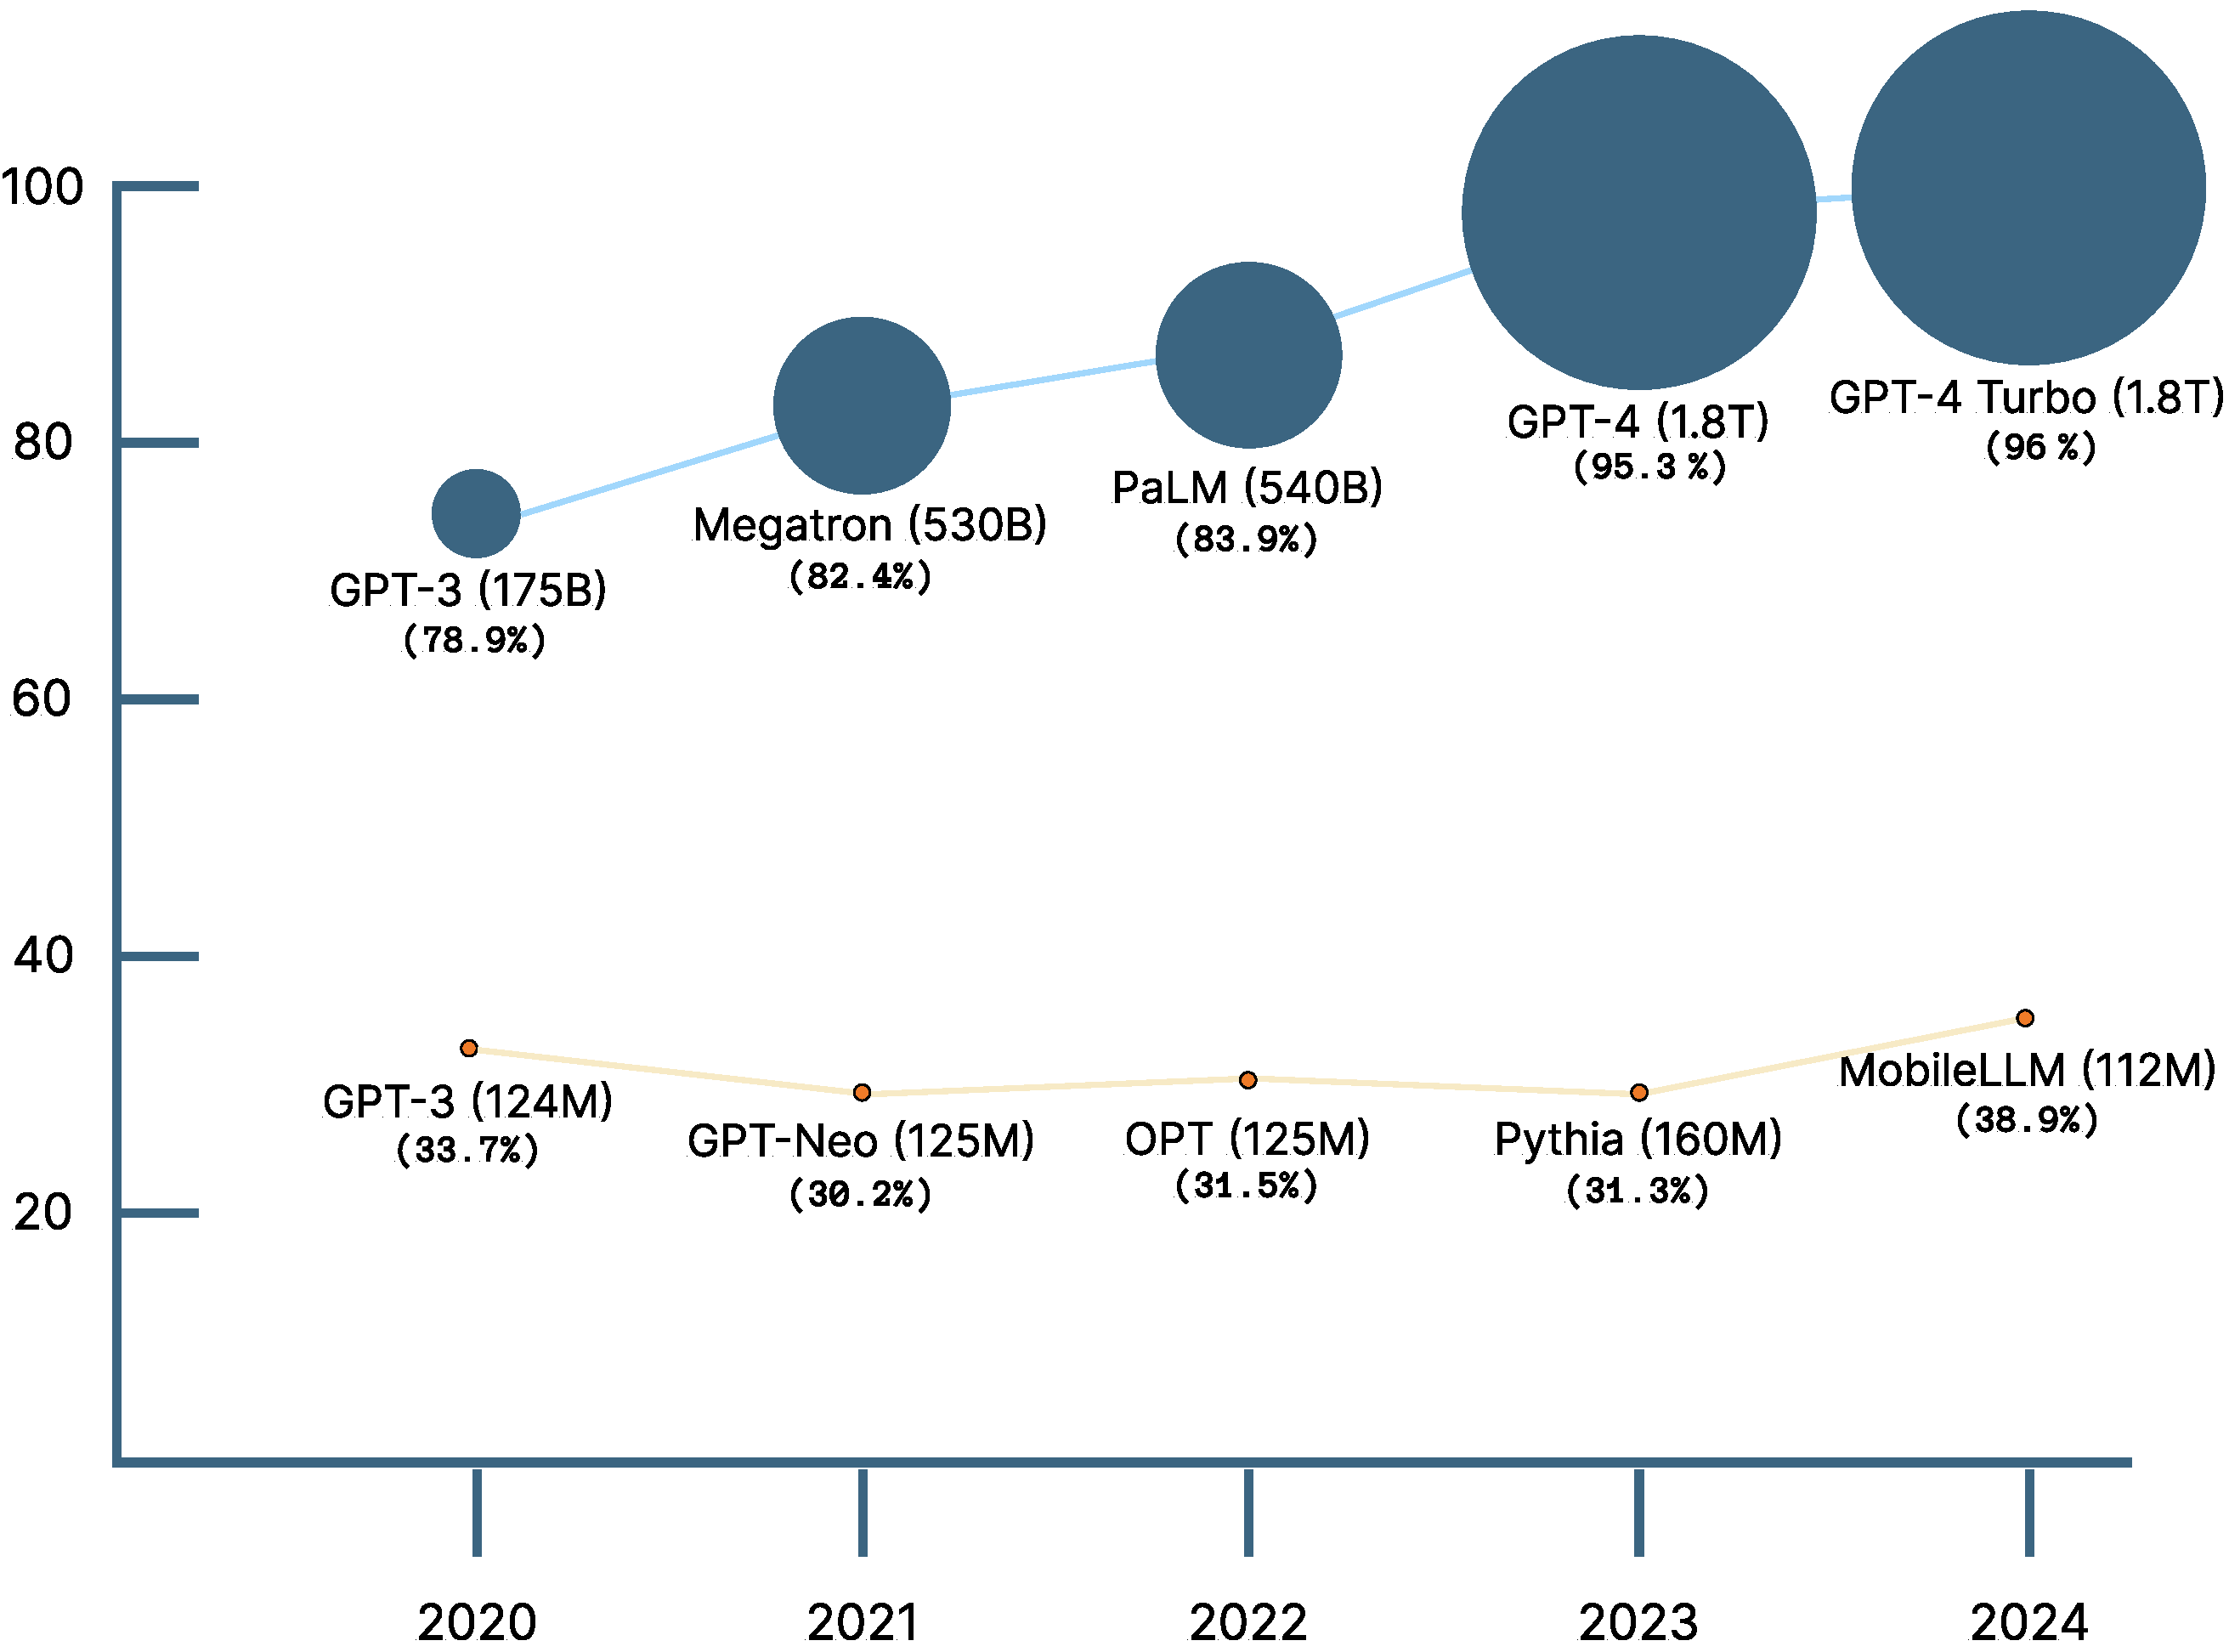
\includegraphics[width=0.8\textwidth]{chapters/introduction/figures/lm_performance_comparison.pdf}
    \caption{Performance of small and large language models on the HellaSwag dataset over time. The plot reveals a striking divergence: while \textbf{\textcolor[HTML]{37718E}{large}} models show consistent improvement, \textbf{\textcolor[HTML]{FF7F11}{small}} models of fixed size (e.g. 100M parameters) have plateaued despite advances in training techniques.}
    \label{fig:model_size_vs_performance}
\end{figure}

This insight extends beyond academic interest. While frontier models dominate public and industrial attention, small language models remain vital for several reasons. %They are not only essential for deployment in resource-constrained environments—such as mobile devices and edge computing—but also play a critical role in enabling transparency, reducing costs, and improving accessibility across a wider range of applications.

\section*{Why Do Small Models Matter?}

% We should also probably define what we mean by small models.

The rapid scaling of language models has brought about remarkable capabilities, but it has also surfaced a host of challenges and risks \citep{bommasani2021foundation}. Small language models, \textit{which we define as models with fewer than 1 Billion (1B) parameters}, offer a promising counterbalance. While the distinction between small and large models is relative to the scale being compared, the 1B parameter threshold provides a practical cutoff: a model with 1B parameters requires approximately 8GB of memory (assuming 32-bit precision) and can therefore be managed on a single GPU or deployed on-device with the hardware available as of 2025. Models of this scale offer several key benefits over their large counterparts:

\paragraph{Large models introduce significant societal risks.} As enumerated by the Stanford Center for Research on Foundation Models \citep{bommasani2021foundation}, these include the potential for generating disinformation and misinformation at scale, amplifying biases and discrimination present in training data, and memorising and regurgitating sensitive or copyrighted content. The wide-spread adoption of these models across industries also raises concerns about the creation of single points of failure: a widely deployed model that is compromised could have cascading negative effects across all downstream applications. Relatedly, the authors highlight that these risks are not just technical but also social, as they can entrench power in the hands of a few organisations and make it harder to adapt models to specific or local needs.

\paragraph{Large models pose serious environmental sustainability challenges.} Researchers have increasingly emphasised energy efficiency as a core evaluation metric, on par with traditional measures like accuracy \citep{schwartz2020greenai}. Studies have quantified the financial and carbon costs of training state-of-the-art NLP systems, revealing orders-of-magnitude differences between large and small models \citep{strubell2019energy}. Tools like the ML Emissions Calculator \citep{lacoste2019quantifying} and systematic reviews of emissions factors \citep{luccioni2023counting} have made it clear that model size, hardware, and training recipes all play a role in determining the environmental footprint of machine learning. Transformer-based models \citep{vaswani2017attention}, in particular, are among the most energy-intensive, given their dense feed-forward architectures. Benchmarks such as HULK \citep{zhou2021hulk} have compared pretrained models' energy efficiency, showing that inducing sparsity and pruning models to reduce their size yields large environmental efficiency. Furthermore, the geographic location where models are trained can significantly affect emissions \citep{patterson2021carbon}; small models that can be trained locally remove the networking cost of distributed, remote model training and serving required by large models. 

%The overall trend is clear: smaller models are more sustainable, and their adoption is crucial for reducing AI's environmental impact.
% For example, a modest increase in translation accuracy can result in a dramatic rise in compute cost.

\paragraph{Data privacy and memorization risks are heightened in large models.} Research has shown that neural networks, especially large ones, can memorize and regurgitate rare or sensitive training data \citep{feldman2020neural, carlini2019secret}. Follow-up studies have demonstrated that memorization increases with model size and data duplication \citep{carlini2021extracting, carlini2022quantifying}; in particular, larger models are more likely to leak personally identifiable information, especially when trained on duplicated or low-diversity data \citep{huang2022large, neel2023privacy}. Recent so-called `scaling laws for memorization' have quantified the relationship between model size and their propensity to memorize and leak sensitive information \citep{lu2024scaling, biderman2023emergent, kiyomaru2024comprehensive}. Mitigation strategies such as differential privacy \citep{dwork2006calibrating} and federated learning \citep{mcmahan2017communication} have been proposed, but these often come with trade-offs in model utility.% In contrast, smaller models by having less capacity to memorize and that can be managed locally offer a more privacy-preserving alternative—especially when combined with privacy-focused training techniques.
% TODO: Edit last sentence

\paragraph{Small models are uniquely suited for on-device and edge deployment.} Efficient inference with limited memory is essential for running language models on consumer hardware. Sub-billion parameter models are particularly important for energy-efficient, on-device applications, as demonstrated by \citet{liu2024mobilellm}. Early advances in mobile-friendly neural network architectures, such as MobileNets \citep{howard2017mobilenets} and EfficientFormer \citep{li2022efficientformer}, laid the groundwork for efficient models in both vision and language domains. More recently, research teams from cellphone manufacturers like Apple and Google have spear-headed efforts to optimise mobile-first models, with efforts to optimise the memory bandwidth of on-device language models \citep{alizadeh2024llm} and build custom hardware accelerators for serving models \citep{deepmind2023gemini}. %The importance of energy-proportional memory for datacenter and mobile applications has also been highlighted \citep{malladi2012towards}. 
 

\paragraph{Interpretability and scientific understanding are reasons to prioritize small models.} The internal mechanisms of transformers and other neural architectures are more tractable in smaller models, making them better testbeds for developing scientific understanding \citep{elhage2021mathematical, elhage2022toy, anthropic2023components}. Tools such as influence functions are easier to apply at small scale, and the "manifold hypothesis" suggests that neural representations of language models (including those of larger models) often exist on a small manifold of the representational space \citep{olah2014manifolds}. More generally, as advocated for by \citet{elhage2021mathematical}, progress in understanding larger models often begins with insights gained from studying the structure of neural representations in smaller models.

\paragraph{The democratization and accessibility of language technology depend on the availability of small, open models.} The cost of training and deploying large models is rising rapidly, with the financial and hardware requirements putting them out of reach for most organisations and individuals \citep{cottier2024rising, sharir2020cost}. Minimal, and small-scale implementations of language models like nanoGPT \citep{karpathy2023nanogpt} and Pico (introduced in Chapter 7) make language modeling accessible to a broader community, supporting experimentation, and innovation. By lowering the barrier to entry, small models enable more researchers to participate in the development and application of language technologies.

% In summary, small language models matter because they are more sustainable, privacy-preserving, interpretable, and accessible. They offer a practical and ethical path forward for language technology, especially as the risks and costs of large-scale models continue to mount.

\section*{Research Objectives}

This thesis aims to explore how small language models can be trained more efficiently and effectively using principled approaches, rather than brute-force scaling. The work is structured around two central research objectives:

\begin{quote}
    \textbf{Research Question 1 (RQ1): Can insights from human language acquisition be leveraged to develop more principled and effective training paradigms for small language models?}
\end{quote}

Despite recent advances in architecture design and model size compression techniques, small models continue to lag behind their larger counterparts. A persistent challenge is that many of the methods proposed to improve small models, ranging from ad hoc architectural tweaks to various forms of regularisation or data augmentation, often lack a strong scientific foundation. Progress is frequently incremental and difficult to interpret; new techniques sometimes offer only marginal gains or fail to generalize beyond specific benchmarks. Without a principled framework or guiding thesis, it becomes challenging to systematically understand what works, why it works, and how to build on prior results in a cumulative way.

One promising guiding thesis is to look to human language acquisition for inspiration. While today's large language models are trained on trillions of tokens, a typical 13-year-old human has been exposed to only around 100 million words \citep{warstadt2023babylm1}. This dramatic discrepancy highlights a key inefficiency in current training paradigms and suggests an opportunity: do strategies that work well for the human brain also confer advantages in artificial models? And can cognitive science offer a roadmap toward more efficient language modeling?

By grounding small model training in insights from human cognition, this thesis seeks to move beyond ad hoc heuristics and toward a more principled, theory-driven foundation. The goal is to understand how cognitive strategies, such as curriculum learning, inductive biases, and compositional generalisation, translate into practical improvements in model design and training. In doing so, this work aims to bridge the gap between machine learning and cognitive science, offering not only empirical results but also conceptual tools for building small language models that are both efficient and robust.

To complement this exploration of training strategies, the second research objective focuses on understanding the learning dynamics of small models more deeply and rigorously.

\begin{quote}
    \textbf{Research Question 2 (RQ2): How can we more quantitatively understand how small models learn and how can we use this understanding to improve model design and training?}
\end{quote}

Improving training efficiency is only part of the broader challenge. Equally important is developing a deeper understanding of the underlying learning dynamics that drive how language models learn: How can we quantitatively study the learning process of language models? And how can we characterise the differences in learning between small and large models in a systematic, interpretable way? These questions demand not just better engineering, but a more scientific, principle-driven approach to model understanding.

In recent years, efforts to improve small language models have often relied on empirical heuristics that offer marginal gains. This trial-and-error mindset obscures the mechanisms behind success and makes it difficult to generalize progress across tasks or domains. 

To make progress, we must focus on the learning process itself: how knowledge is acquired, how model capacity is structured and used, and how different factors shape convergence dynamics. Small models provide a unique lens for this investigation not only because they are easier to analyse, but because their behaviour often reveals the underlying structure of learning in ways large models conceal.

This research objective, therefore, is grounded in the belief that meaningful progress in model development must be built on a deeper understanding of the learning process itself. By focusing on measurable, interpretable properties of training, such as model convergence dynamics and representational capacity, we can turn language model development into a more principled science. Furthermore, by developing tools that enable the analysis and understanding of the learning dynamics of small models, we can develop a more principled approach to model development; rather than relying on trial-and-error, we can systematically test and evaluate different training strategies and interventions and study how these affect the learning process of small models. Building tools and frameworks that make the process of developing small models more scientific and accessible to a broader audience is a key goal of this thesis.

\section*{Thesis Overview}

This thesis is organised into two parts, reflecting the two research threads:

\subsection*{Part I: Cognitive Insights for Efficient Training (Chapters 2–4)}

\begin{itemize}

    \item \textbf{Chapter 2:} \emph{Language Modeling: Foundations, Scale, and Efficiency} offers both an overview of the development and current state of language modelling, and a review of the major strategies for training language models more efficiently. The chapter first introduces foundational concepts in language modelling that are used throughout the thesis. I then review existing strategies for training language models more efficiently; from architectural innovations, optimization techniques, and data calibration methods. I conclude by drawing connections between machine learning and cognitive science, considering how insights from human language acquisition can inform more principled model development, especially in resource-constrained environments.

    \item \textbf{Chapter 3:} \emph{Curriculum Learning for Infant-inspired Model Building: A Framework for Human-like Language Acquisition}  
    explores a systematic investigation of curriculum learning strategies inspired by human language acquisition, focusing on their application to small language models. The work is motivated by the striking data efficiency of human language learning compared to current language models.

    The chapter introduces \climb, a framework that operationalises three key aspects of human language acquisition into a curriculum learning framework: a vocabulary curriculum that gradually expands a model's lexicon, a data curriculum that orders training inputs by linguistic complexity and an objective curriculum that transitions from coarse word-class prediction to fine-grained masked language modelling.

    Using the BabyLM Challenge's strict 10-million-word training cap as a testbed, this work develops an optimised "vanilla" BabyBERTa baseline that we use as a benchmark against the three curriculum learning approaches. The empirical results reveal that while individual curricula do not consistently outperform this baseline, they offer selective advantages when combined together and on specific linguistic tasks, particularly in syntactic evaluation.

    \item \textbf{Chapter 4:} \emph{Learning Words Like Humans Do: Syntactic Smoothing for Language Model Training}  
    explores how language models can learn word representations more like humans do, by leveraging syntactic structure to improve the representation of infrequent tokens. This work addresses a fundamental challenge in language modelling: while humans are able to leverage the linguistic structure of language to quickly learn new words, language models struggle to effectively represent tokens that appear rarely in their training data. This inefficiency stems from the maximum likelihood training objective, which disproportionately optimises frequent tokens while leaving infrequent ones with insufficient learning signals. In contrast to human language acquisition, language models learn frequency statistics that results in infrequent tokens being pushed into a narrow manifold of the representational space (a phenomenon known as `anisotropy'). 
    In this chapter, we show that this training process leads models to encode, what we label, a `frequency bias' and provide a mechanism for quantifying this bias. Next, inspired by how humans leverage syntactic knowledge to learn new words efficiently, we introduce \smoothing, a novel technique that improves token representations by incorporating linguistic structure into the learning process. By using part-of-speech distributions as a proxy for syntactic similarity this method enables infrequent tokens to benefit from the learning signals of syntactically similar tokens. This approach mirrors the way humans use syntactic knowledge to learn new words efficiently and demonstrates how insights from human language acquisition can lead to more principled and effective training paradigms for language models.

\end{itemize}

\subsection*{Part II: An Analytical Lens on Learning Dynamics (Chapters 5-7)}

\begin{itemize}
    \item \textbf{Chapter 5:} \emph{Analyzing Language Models: Foundations, Methods, and Tools} introduces the analytical foundations for studying the learning dynamics of language models. I present a range of complementary approaches for analysing these dynamics, including memorisation and data influence methods, representational convergence and similarity metrics (such as CKA and model stitching), and capacity usage via sparsity, norm evolution, and rank-based analysis. These tools can be used to reveal how internal structures in language models develop, and how the learning trajectories of smaller models diverge from their larger counterparts.

    The chapter also situates this analysis within the broader interpretability literature, like attention pattern analysis, probing methods, and mechanistic interpretability. This background chapter lays the groundwork for the next two chapters, which apply these tools to understand and intervene in the learning dynamics of small language models.

    \item \textbf{Chapter 6:} \emph{Tending Towards Stability: Convergence Challenges in Small Language Models} examines why small language models often exhibit unstable or delayed convergence during training. I use the Pythia model suite to compare learning dynamics across model sizes, focusing on how internal layer activations evolve and how efficiently models use their representational capacity.

    I apply Centered Kernel Alignment (CKA) to track the convergence of activations over time and introduce Proportional Effective Rank (PER) as a new metric to assess how layers utilise their parameters and gradients. My findings show that larger models converge more quickly and consistently, while smaller models underutilise capacity, leading to erratic learning and premature saturation.
    
    These results suggest that small models suffer from inefficient learning trajectories, not just limited capacity. The chapter closes by identifying the need for an intervention-friendly training framework to test hypotheses about improving small model training which motivates the design of the \pico framework presented in Chapter 7.

    \item \textbf{Chapter 7:} \emph{\pico: A Lightweight Framework for Studying Language Model Learning Dynamics} introduces \pico, a modular framework designed to support the scientific development of language models.

    \pico consists of two core components:
    
    \begin{enumerate}
        \item \texttt{pico-train}, a minimalist training library that logs model weights, activations, and gradients at regular intervals, and
        
        \item \texttt{pico-analyze}, a companion toolkit that computes metrics such as PER, CKA, sparsity, and norm dynamics across layers and checkpoints.
    \end{enumerate}

    Together, these tools enable researchers to systematically explore how architectural or training interventions affect learning dynamics. A typical workflow involves formulating a hypothesis, implementing the corresponding modification in \texttt{pico-train}, and using \texttt{pico-analyze} to evaluate its effects. This creates a feedback loop for iterative, and systematic model development. This chapter presents several case studies to illustrate how \pico supports this process in practice.

\end{itemize}

\section*{Contributions}

This thesis makes the following contributions to the study of small language models, with a two-part emphasis on efficient training and principled model understanding:

\vspace{1em}

\textbf{1. Cognitively inspired training strategies for small language models}

\begin{itemize}

    \item Presents \climb, a three-pronged curriculum learning framework based on principles from human language acquisition. \climb both defines and operationalises three forms of curriculum learning that operate on the vocabulary, input data, and objective function. While these strategies are intuitively appealing, I find that they offer limited benefit in practice, making \climb a comprehensive and critical evaluation of human-inspired curricula for language model training. (Chapter 3).

    \item Proposes \smoothing, a cognitively motivated method that mimics how humans use grammatical structure to infer the meaning of rare words. By diffusing learning signals across syntactically similar tokens, the approach reduces frequency bias and improves representation of low-frequency words. (Chapter 4).

\end{itemize}

\textbf{2. A quantitative framework for analyzing learning dynamics in small models}

\begin{itemize}
    \item Introduces a set of metrics for quantifying both how effectively layers in a language model use their representational capacity over time and how well a model converges to a stable representation (Chapter 6).

    \item Applies these metrics to show that small models converge more slowly and inconsistently than larger models due to inefficient internal capacity usage.

\end{itemize}

\textbf{3. An open-source platform for training-time analysis and reproducible experimentation}
\begin{itemize}
    \item Presents \textbf{\pico}, a modular framework for developing language models in a scientific, hypothesis-driven way. \pico integrates two libraries that enable researchers to iteratively train and analyse language models in a systematic and reproducible way. (Chapter 7).

    \item Releases the \textbf{\pico Model Suite}, a family of small- to mid-sized models (11M–-570M parameters) trained with standardised recipes and full checkpoint access that can be used as a starting point for scaling studies, and interpretability research.
\end{itemize}

\newpage
\section*{Publications}

The content of this thesis is comprised of the following published conference papers and software packages.

\begin{tcolorbox}[
    enhanced,
    colback=white,
    colframe=thesisblue,
    arc=0mm,
    boxrule=1pt,
    left=10pt,
    right=10pt,
    top=10pt,
    bottom=10pt,
    title=Published Works,
    fonttitle=\bfseries,
    coltitle=white
]
\subsection*{Thesis Publications}
The following papers and software packages form the core content of this thesis.

\begin{itemize}
    \item Richard Diehl Martinez, Zebulon Goriely, Hope McGovern, Christoper Davis, Andrew Caines, Paula Buttery, Lisa Beinborn (2023). {\color{thesisblue}\href{https://aclanthology.org/2023.conll-1.10/}{CLIMB – Curriculum Learning for Infant-inspired Model Building}}. In \emph{Proceedings of the BabyLM Challenge at the 27th Conference on Computational Natural Language Learning}, pages 138-154, Singapore. Association for Computational Linguistics.

    \item Richard Diehl Martinez, Zebulon Goriely, Andrew Caines, Paula Butery, Lisa Beinborn (2024). {\color{thesisblue}\href{https://aclanthology.org/2024.emnlp-main.486/}{Mitigating Frequency Bias and Anisotropy in Language Model Pre-Training with Syntactic Smoothing}}. In \emph{Proceedings of the 2024 Conference on Empirical Methods in Natural Language Processing}, pages 8541-8565, Miami, Florida, USA. Association for Computational Linguistics.

    \item Richard Diehl Martinez, Pietro Lesci, Paula Buttery (2024). {\color{thesisblue}\href{https://aclanthology.org/2024.findings-emnlp.246/}{Tending Towards Stability: Convergence Challenges in Small Language Models}}. In \emph{Findings of the Association for Computational Linguistics: EMNLP 2024}, pages 4253-4263, Miami, Florida, USA. Association for Computational Linguistics.

    \item Richard Diehl Martinez, David Demitri Africa, Yuval Weiss, Suchir Salhan, Ryan Daniels, Paula Buttery (2025). {\color{thesisblue}\href{https://github.com/pico-lm}{Pico: A Modular Framework for Hypothesis-Driven Small Language Model Research}}. In Submission to \emph{2025 Conference on Empirical Methods in Natural Language Processing System Demonstration Track}.
\end{itemize}
\end{tcolorbox}

\newpage

\begin{tcolorbox}[
    enhanced,
    colback=white,
    colframe=thesisblue,
    arc=0mm,
    boxrule=1pt,
    left=10pt,
    right=10pt,
    top=10pt,
    bottom=10pt,
    title=Additional Works,
    fonttitle=\bfseries,
    coltitle=white
]
\subsection*{Mentored Works}
I mentored the following projects during my PhD.

\begin{itemize}
    \item David Demitri Africa, Yuval Weiss, Paula Buttery, Richard Diehl Martinez (2025). {\color{thesisblue}{Learning Dynamics of Meta-Learning in Small Model Pretraining}}. In Submission to \emph{BlackBox Workshop at the 2025 Conference on Empirical Methods in Natural Language Processing}.
    \item Yuval Weiss, David Demitri Africa,  Paula Buttery, Richard Diehl Martinez (2025). {\color{thesisblue}{Investigating ReLoRA: Effects on the Learning Dynamics of Small Language Models}}. In Submission to \emph{BlackBox Workshop at the 2025 Conference on Empirical Methods in Natural Language Processing}.
    \item David Demitri Africa, Yuval Weiss, Paula Buttery, Richard Diehl Martinez (2025). {\color{thesisblue}{Filipino Zero-Shot Transfer Using Meta-Pretraining for Named Entity Recognition}}. In Submission to \emph{Multilingual Representation Learning Workshop at the 2025 Conference on Empirical Methods in Natural Language Processing}.
\end{itemize}

\subsection*{Other Publications}
I also worked on the following papers during my PhD (not included in this thesis).

\begin{itemize}
    \item Cole Simmons, Richard Diehl Martinez, Dan Jurafsky (2024). {\color{thesisblue}\href{https://aclanthology.org/2024.ml4al-1.20/}{SumTablets: A Transliteration Dataset of Sumerian Tablets}}. In \emph{Proceedings of the 1st Workshop on Machine Learning for Ancient Languages}, pages 192-202, Bangkok, Thailand. Association for Computational Linguistics.
    \item Zebulon Goriely, Richard Diehl Martinez, Andrew Caines, Paula Buttery, Lisa Beinborn (2024). {\color{thesisblue}\href{https://aclanthology.org/2024.conll-babylm.4/}{From Babble to Words: Pre-Training Language Models on Continuous Streams of Phonemes}}, In \emph{Proceedings of the BabyLM Challenge at the 27th Conference on Computational Natural Language Learning}, pages 37-53, Miami, Florida, USA. Association for Computational Linguistics.
    \item Suchir Salhan, Richard Diehl Martinez, Zebulon Goriely, Paula Buttery (2024). {\color{thesisblue}\href{https://aclanthology.org/2024.conll-babylm.15/}{Less is More: Pre-Training Cross-Lingual Small-Scale Language Models with Cognitively-Plausible Curriculum Learning Strategies}}, In \emph{Proceedings of the BabyLM Challenge at the 27th Conference on Computational Natural Language Learning}, pages 174-188, Miami, Florida, USA. Association for Computational Linguistics.
    % \item  Richard Diehl Martinez$^{\dagger}$, Suchir Salhan$^{\dagger}$, Zebulon Goriely, Paula Buttery (2025). {\color{thesisblue}{How Long Can a \textsc{BabyLM} Go? Investigating the Effect of Sequence Length on Small Language Model Pre-Training}}. In Submission to \emph{2025 BabyLM Workshop at the Conference on Empirical Methods in Natural Language Processing}. $^{\dagger}$Equal contribution.
\end{itemize}
\end{tcolorbox}


% PART 1 

\part{Cognitive Insights for Efficient Training}

% Background section
\chapter{Language Modeling Background and Small Language Models}

In this chapter, we will explore the background of language modeling, including the early approaches, word embeddings, and language models, leading up to current state of the art large language models. We will then pivot and outline some of the methods that researchers have used to make progress on efficiently training small language models. 

\section{Language Modeling Task}

Language modeling refers to the task of assigning probabilities to sequences of words or tokens. The goal is to model the likelihood of a sequence in a language. In the case of a sequence of words, $w = w_1, w_2, \ldots, w_n$, the probability of the sequence is given by the product of the probabilities of the words occurring in the sequence:

\begin{equation}    
    P(w) = P(w_1, w_2, \ldots, w_n) = \prod_{i=1}^n P(w_i | w_1, \ldots, w_{i-1})
\end{equation}

Training a language model is then equivalent to estimating the parameters of this probability distribution. In practice, this is done by estimating the parameters of a neural network that maps a sequence of words to a probability distribution over the next word. 

\subsection{Early Approaches: N-Gram Models}
The earliest language models were based on n-gram statistics, where the probability of a word depends only on the preceding $n-1$ words. These models, described in foundational texts such as \cite{jurafsky2025speech}, are simple and effective but suffer from data sparsity and limited context. To address these issues, various smoothing techniques were developed, including Katz backoff \citep{katz2003estimation} and Kneser-Ney smoothing \citep{kneser1995improved}, with interpolated Kneser-Ney \citep{chen1999empirical} becoming the de facto standard for n-gram language modeling.

\subsection{Neural Language Models}

A major breakthrough came with the introduction of neural probabilistic language models by \cite{bengio2003neural}, which proposed using feed-forward neural networks to estimate the probability of word sequences. This approach introduced distributed word representations (embeddings), alleviating the data sparsity problem inherent in n-gram models. Subsequent work explored more powerful architectures, such as recurrent neural networks (RNNs) \citep{mikolov2010recurrent}, which can, in principle, capture dependencies across arbitrarily long contexts. However, training RNNs is challenging due to the vanishing and exploding gradient problems \citep{bengio1994learning}, leading to the development of gated architectures like Long Short-Term Memory (LSTM) networks \citep{hochreiter1997lstm} and Gated Recurrent Units (GRUs) \citep{cho2014gru}.
Large-scale empirical studies, such as \cite{jozefowicz2016exploring}, benchmarked various neural architectures and demonstrated that both model architecture and training data size significantly impact language modeling performance, as measured by perplexity.
\subsection{Word Embeddings}
In parallel, the adoption of distributed word representations, or word embeddings, marked a paradigm shift in NLP. Methods such as Skip-gram and Continuous Bag-of-Words (CBOW) \citep{mikolov2013efficient, mikolov2013distributed} and GloVe \citep{pennington2014glove} learn dense vector representations that capture syntactic and semantic relationships between words. These embeddings enabled transfer learning in NLP, as pre-trained vectors could be used for a variety of downstream tasks, including named entity recognition~\citep{lample2016neural}, sentence classification~\citep{kim2014convolutional}, and machine translation~\citep{qi2018translation}. However, traditional word embeddings are static, assigning the same vector to a word regardless of context.

Some novel methods have attempted to preproces or represent the input text data in unique ways, such as \cite{kim2016character} and phoneme-level representations \cite{goriely2024babble}.

\subsection{Contextualization and Attention}
To address the limitations of static embeddings, attention mechanisms were introduced, initially to solve the sequence alignment problem in machine translation \citep{bahdanau2015neural,luong2015effective}. Attention allows models to dynamically focus on relevant parts of the input sequence, improving translation quality and enabling the development of encoder-decoder architectures \citep{sutskever2014sequence}. The concept of contextual word embeddings was further advanced by models such as ELMo \citep{peters2018deep}, which extract context-sensitive representations from deep, bidirectional LSTMs.

\subsection{The Transformer and Modern Language Models}
The introduction of the Transformer architecture by Vaswani et al.~\citep{vaswani2017attention} marked a turning point in language modeling by replacing recurrence with self-attention mechanisms. This enabled efficient parallelization and the modeling of long-range dependencies, setting new performance benchmarks in machine translation and other NLP tasks. The Transformer built on earlier advances such as the soft attention mechanism of Bahdanau et al.~\citep{bahdanau2015neural}, which allowed neural machine translation models to dynamically align source and target sequences, improving translation quality and eliminating the need for a fixed-size encoding.

BERT~\citep{devlin2019bert} introduced the masked language modeling (MLM) objective, where some percentage of input tokens are replaced with a special [MASK] token, and the model is trained to predict the original identity of these masked tokens given their context. Formally, for a sequence of tokens $w = (w_1, \ldots, w_n)$ and a set of masked positions $M \subset \{1, \ldots, n\}$, the MLM objective maximizes
\begin{equation}
    \mathcal{L}_{\text{MLM}} = \sum_{i \in M} \log P(w_i \mid w_{\setminus M}),
\end{equation}
where $w_{\setminus M}$ denotes the sequence with masked tokens replaced by [MASK]. This enables BERT to learn deep bidirectional representations, as the model can attend to both left and right context. 

Following BERT, a number of variants improved on its design. RoBERTa~\citep{liu2019roberta} removed the next sentence prediction task and scaled up training data and compute. ALBERT~\citep{lan2019albert} introduced parameter sharing and sentence order prediction to reduce model size and improve efficiency. SpanBERT~\citep{joshi2020spanbert} focused on span-level objectives for better performance on related tasks. Other architectural innovations include DistilBERT~\citep{sanh2019distilbert}, which compresses BERT via knowledge distillation, and DeBERTa~\citep{he2021deberta}, which enhances attention mechanisms through disentangled representations.

In contrast to masked language modeling, autoregressive pretraining—as used in the GPT series~\citep{radford2018gpt1, radford2019gpt2, brown2020gpt3}—trains models to predict each token based only on its preceding context. This objective maximizes the likelihood:

\begin{equation}
\mathcal{L}_{\text{AR}} = \sum_{i=1}^n \log P(w_i \mid w_1, \ldots, w_{i-1}),
\end{equation}

enforcing a unidirectional, left-to-right dependency. Despite this constraint, autoregressive models have proven particularly effective for large-scale pretraining, and form the foundation of many state-of-the-art language models used today. Their simplicity and scalability have contributed to their widespread adoption for open-ended generation tasks.

Building on these two main paradigms, several models have explored alternative objectives and architectures. One especially influential direction is the encoder-decoder, or text-to-text, framework. T5~\citep{raffel2020t5} exemplifies this approach by casting all NLP tasks—classification, translation, question answering—as text generation problems within a unified pretraining scheme. Similarly, BART~\citep{lewis2020bart} combines a denoising autoencoder objective with a sequence-to-sequence architecture, enabling both robust understanding and fluent generation.

Other notable innovations include Transformer-XL~\citep{dai2019transformer}, which improves long-context modeling through segment-level recurrence and relative positional encodings; CTRL~\citep{keskar2019ctrl}, which allows controllable generation via conditioning on control codes; ELECTRA~\citep{clark2020electra}, which reframes pretraining as a discriminative task of replaced-token detection for improved sample efficiency; and XLNet~\citep{yang2019xlnet}, which generalizes autoregressive modeling using permutation-based objectives to capture bidirectional dependencies without masking.

Together, these advances reflect a broad exploration of architectures and training strategies, enabling the current generation of language models to achieve impressive results across a wide range of NLP tasks.

\subsection{Alternative Architectures}
While Transformers dominate large language modeling, recent research has explored alternative sequence modeling approaches to address their limitations, such as quadratic complexity and long-range dependency challenges. One promising direction is state space models (SSMs). The HiPPO framework~\citep{gu2020hippo} introduced efficient memory representations for continuous-time sequences, leading to the Structured State Space Sequence (S4) model~\citep{gu2021efficiently}, which models long-range dependencies efficiently via fast convolution. Mamba~\citep{gu2023mamba} further advances SSMs with dynamic, input-dependent state transitions, achieving Transformer-level performance with linear complexity. Another notable architecture, RWKV~\citep{peng2023rwkv}, combines features of Transformers and RNNs, replacing self-attention with a time-mixed mechanism for efficient, competitive language modeling. 

While these alternative architectures represent novel and important directions for efficient and expressive sequence modeling, in this thesis we focus primarily on Transformer-based models as the most successful and widely adopted approach for language modeling.

\subsection{Training and Optimization}

\paragraph{Optimization Algorithms.} The foundational method for training neural networks is stochastic gradient descent (SGD)\citep{robbins1951stochastic}, which iteratively updates model parameters using noisy gradient estimates from mini-batches. To address limitations in learning rate tuning and convergence speed, a range of adaptive optimizers have been developed. These include Adagrad\citep{duchi2011adaptive}, which adapts learning rates based on historical gradients; RMSProp~\citep{tieleman2012lecture}, which normalizes updates using a moving average of squared gradients; Adam~\citep{kingma2015adam}, which combines momentum with adaptive learning rates; and AdamW~\citep{loshchilov2019decoupled}, which decouples weight decay from the gradient update, improving regularization behavior.
In practice, effective training of deep networks also relies on learning rate scheduling and gradient clipping. For example, the Transformer architecture~\citep{vaswani2017attention} employs a learning rate schedule with an initial warm-up phase followed by inverse square root decay. Additionally, gradient clipping~\citep{pascanu2013difficulty}—scaling gradients when they exceed a threshold—is essential for preventing exploding gradients, a technique that has proven crucial for training recurrent neural networks and stabilizing large-scale Transformer models.

\paragraph{Activation Functions.} 

An activation function is a mathematical operation applied to each neuron's output in a neural network, introducing nonlinearity and enabling the network to learn complex patterns. Activation functions are central to the expressiveness and trainability of neural networks. Early neural networks, as in the foundational work on backpropagation~\citep{rumelhart1986learning}, primarily used the sigmoid activation. \citet{lecun1998efficient} analyzed practical choices for activations, showing that $\tanh$ is preferable to sigmoid due to its zero-centered output, which improves optimization dynamics.

However, both sigmoid and $\tanh$ suffer from vanishing gradients in deep networks, as highlighted by \citet{glorot2010understanding}. This limitation motivated the adoption of the Rectified Linear Unit (ReLU)~\citep{nair2010rectified}, defined as $\mathrm{ReLU}(x) = \max(0, x)$, which is computationally simple and alleviates vanishing gradients. ReLU became the default activation in deep learning throughout the 2010s and is still used in some lightweight transformer variants. Variants such as Leaky ReLU~\citep{maas2013rectifier} allow a small gradient for negative inputs, helping to prevent the ``dying ReLU'' problem, and have seen use in audio and speech models.

For modern language models, smoother and non-monotonic activations have proven more effective. The Gaussian Error Linear Unit (GELU)~\citep{hendrycks2016gaussian} became the default in BERT and subsequent transformers due to its empirical gains over ReLU. Swish~\citep{ramachandran2017searching}, defined as $\mathrm{Swish}(x) = x \cdot \mathrm{sigmoid}(\beta x)$, is another smooth, non-monotonic activation that performs well in deep and convolutional models. More recently, gated activations such as SwiGLU~\citep{shazeer2020glu}—which combines Swish and linear units—have outperformed ReLU and earlier GLU variants in transformer feedforward networks.

The evolution of activation functions reflects the ongoing search for improved expressiveness, optimization, and stability in deep neural architectures.

\paragraph{Regularization and Stabilization.} Overfitting occurs when a model learns not only the underlying patterns in the training data but also the noise, resulting in poor generalization to new, unseen data. To address this, regularization techniques such as dropout~\citep{srivastava2014dropout} are employed, which randomly deactivate units during training to encourage robustness and prevent reliance on specific features.

In addition to regularization, normalization methods play a crucial role in stabilizing training and further improving generalization. \textbf{Batch Normalization}~\citep{ioffe2015batchnorm} normalizes activations over a mini-batch, but is less common in language models due to variable sequence lengths. Instead, \textbf{Layer Normalization}~\citep{ba2016layernorm} is widely used in RNNs and Transformers, as it normalizes across features within each data point, improving stability regardless of batch size. \textbf{RMSNorm}~\citep{zhang2019rmsnorm}, a simplified variant omitting mean subtraction, is used in models like T5 and GPT-J. The placement of normalization layers has evolved: the original Transformer~\citep{vaswani2017attention} used \emph{Post-LN} (after residuals), but this can destabilize deep models. \emph{Pre-LN}~\citep{xiong2020layer}, where normalization is applied before each sublayer, is now standard in most modern LMs for improved stability.

\paragraph{Architectural Enhancements.}
A crucial architectural component in Transformer-based models is the method for encoding token position, which allows models to incorporate sequence order into otherwise permutation-invariant self-attention mechanisms. The original Transformer~\citep{vaswani2017attention} introduced \emph{sinusoidal positional encodings}, which are added to token embeddings and provide a fixed, non-learned way to represent absolute position. In contrast, models such as GPT~\citep{radford2018gpt1} and BERT~\citep{devlin2019bert} use \emph{learned positional embeddings}, which offer greater flexibility but may generalize poorly to longer contexts unless specifically augmented.

To address the limitations of absolute position encodings, \citet{shaw2018self} proposed \emph{relative position representations}, allowing the model to encode the distance between tokens directly in the attention mechanism. This approach is particularly important for enabling models to generalize to longer contexts and to be less dependent on a fixed sequence length. Further innovations include \emph{linear attention biases} (ALiBi)~\citep{press2021train}, which add a simple, non-learned bias to the attention scores based on token distance. Another widely adopted method is the \emph{Rotary Position Embedding} (RoPE)~\citep{su2024rope}, which applies rotary transformations to the key and query vectors in the attention mechanism. RoPE has become popular in many large models, such as LLaMA, due to its strong extrapolation capabilities and implementation simplicity.

Beyond positional encoding, several other architectural enhancements have become standard in modern Transformers. \emph{Residual connections}~\citep{he2016deep}, originally introduced in ResNets to address vanishing gradients, are essential for enabling the training of deep Transformer models by facilitating gradient flow. More recent innovations include \emph{Grouped Query Attention} (GQA)~\citep{ainslie2023gqa}, which reduces memory and compute requirements by grouping multiple attention heads to share key and value projections—a technique now adopted in models such as Gemini, PaLM, and LLaMA. Additionally, parameter efficiency has been improved through \emph{weight tying}~\citep{press2017using}, where the input and output embedding matrices are shared, reducing the number of parameters without sacrificing performance

\subsection{Scaling and Architecture Search}
While recent research has shown that scaling model and dataset size leads to predictable improvements in performance~\citep{kaplan2020scaling, henighan2020scaling}, designing neural network architectures in a robust and rigorous way remains a significant challenge. Much of architecture design is still guided by empirical intuition and trial-and-error, rather than first principles. For example, \citet{levine2020depth} offer a structured perspective on the trade-offs between scaling depth and width in Transformers, proposing guidelines for balancing these factors under a fixed compute budget. The scaling laws established by \citet{kaplan2020scaling} demonstrate that both wider and deeper models can improve performance if scaled appropriately, but do not prescribe how to select specific architectural configurations for a given task or resource constraint.

To address the difficulty of manual architecture design, neural architecture search (NAS) methods have been developed to automate this process. Early work by \citet{zoph2017neural} introduced the use of reinforcement learning to train a controller network that proposes architectures, using the accuracy of candidate models as a reward signal. More recent approaches have applied NAS specifically to Transformer models: AutoFormer~\citep{chen2021autoformer} efficiently searches over large design spaces (such as number of heads, depth, and MLP size) using weight-sharing, while NAS-BERT~\citep{xu2021nasbert} tailors BERT-like architectures for specific NLP tasks, reducing model size while maintaining performance through task-conditioned optimization.

Despite these advances, finding good architectures remains challenging and is difficult to do rigorously. Automated methods like NAS are increasingly important for discovering efficient and effective models, but robust principles for architecture design are still an open research area.


\section{Large Language Models}

The advent of large language models (LLMs) marked a turning point in natural language processing. Unlike earlier models, which were limited by data and compute, LLMs are trained on massive corpora and contain billions or even trillions of parameters. This scale enables them to perform a wide range of tasks—including question answering, summarization, translation, and code generation—often with little or no task-specific training. It is important to note, however, that the definition of ``large'' in large language models is a moving target: as models and hardware have advanced, what was once considered large has quickly become standard or even small by contemporary benchmarks.

The rapid progress in large language models has been marked by influential systems, each pushing the boundaries of scale, capability, and accessibility. GPT-3~\citep{brown2020gpt3} established the transformative potential of large transformer-based models, enabling tasks in few-shot or zero-shot settings. GPT-4~\citep{openai2023gpt4} further expanded scale and capabilities, emphasizing the complexities of evaluating massive models.

Open-source models have also significantly advanced the field. DeepSeek LLM~\citep{deepseek2024llm} optimizes hyperparameters aligned with scaling laws, while Mistral 7B~\citep{jiang2023mistral} introduces efficiency-driven architectural innovations. Similarly, PaLM~\citep{chowdhery2023palm}, OPT~\citep{zhang2022opt}, and BLOOM~\citep{le2023bloom} contribute distinct approaches to scaling and transparency, with LLaMA models~\citep{touvron2023llama} emphasizing research optimization.

Furthermore, models like Anthropic's Claude~\citep{anthropic2024claude3,anthropic2024claude35,anthropic2025claude37}, Google's Gemini~\citep{deepmind2023gemini}, Baidu's ERNIE 4.0~\citep{baidu2023ernie4}, and Alibaba's Qwen~\citep{alibaba2023qwen} demonstrate advancements in multimodality, language specificity, and principled AI, showcasing diverse avenues of progress in large-scale language modeling.

The following section explores some of the critical aspects of large language models including their pre-training datasets, large-scle evaluation benchmarks, and properties.

\subsection{Datasets for Large Language Model Pretraining}
The performance of large language models (LLMs) is strongly influenced by the scale, diversity, and quality of their pretraining datasets. Over the past several years, a number of large-scale corpora have been developed to support open and reproducible LLM research. Table~\ref{tab:llm-datasets} summarizes some of the most widely used datasets.
\begin{table}[h]
\centering
\begin{tabular}{p{3.5cm} p{1.5cm} p{8.5cm}}
\toprule
\textbf{Dataset} & \textbf{Size} & \textbf{Type of Data} \\
\midrule
OpenWebText~\citep{gokaslan2019openweb} & $\sim$8B & Web, Wikipedia \\
BooksCorpus~\citep{zhu2015aligning} & $\sim$0.8B & Fiction books \\
The Pile~\citep{gao2020pile} & 250B & Web, academic, code, books, forums \\
C4~\citep{raffel2020t5} & 365B & Web (Common Crawl) \\
RedPajama~\citep{together2023redpajama} & 1.2T & Web, books, Wikipedia, code, academic \\
RefinedWeb~\citep{penedo2023refinedweb} & 600B & Web (Common Crawl) \\
FineWeb~\citep{penedo2024fineweb} & 15T & Web, education \\
DOLMa~\citep{soldaini2024dolma} & 3T & Web, Wikipedia, books, code, academic, forums \\
\bottomrule
\end{tabular}
\caption{Major datasets used for large language model pretraining, with approximate number of tokens and data types.}
\label{tab:llm-datasets}
\end{table}
These datasets are constructed from a variety of sources, including web pages (Common Crawl), books, academic papers, code repositories, and community forums. Notably, OpenWebText~\citep{gokaslan2019openweb} and BooksCorpus~\citep{zhu2015aligning} were foundational for early models like GPT-2 and BERT, while The Pile~\citep{gao2020pile} and C4~\citep{raffel2020t5} introduced greater diversity and scale. More recent efforts such as RedPajama~\citep{together2023redpajama}, RefinedWeb~\citep{penedo2023refinedweb}, FineWeb~\citep{penedo2024fineweb}, and DOLMa~\citep{soldaini2024dolma} focus on openness, quality filtering, and massive scale, supporting the next generation of open LLMs.

\subsection{Evaluation Benchmarks for Large Language Models}
The advancemnet of large language models (LLMs) has also been driven by the development of rigorous evaluation benchmarks. These benchmarks assess a model's ability to understand, reason, and generate language across a wide range of tasks. Below, we summarize some of the most influential benchmarks used to evaluate LLMs.
\paragraph{GLUE and SuperGLUE.} The General Language Understanding Evaluation (GLUE) benchmark \citep{wang2018glue} popularized the paradigm of transfer learning and fine-tuning in NLP. It consists of nine tasks, including natural language inference (MNLI, RTE) \citep{williams2018mnli,dagan2006rte}, paraphrase detection (MRPC) \citep{dolan2005mrpc}, sentiment analysis (SST-2) \citep{socher2013sst}, linguistic acceptability (CoLA) \citep{warstadt2019cola} and semantic similarity (STS-B) \citep{cer2017stsb}. BERT's breakthrough performance on GLUE established it as a standard benchmark, but as models approached the performance ceiling, overfitting became a concern. SuperGLUE \citep{wang2019superglue} was introduced as a more challenging successor, featuring tasks that require multi-sentence reasoning, commonsense inference, and coreference resolution \citep{zhang2018record,pilehvar2019wic,khashabi2018multirc,roemmele2011copa}. Progress on these benchmarks has closely tracked advances in LLM capabilities.

\paragraph{MMLU.} The Massive Multitask Language Understanding (MMLU) benchmark \citep{hendrycks2021mmlu} evaluates models on 57 diverse tasks spanning STEM, humanities, law, and more, using multiple-choice questions. MMLU emphasizes zero-shot and few-shot generalization, and is now a standard for evaluating the broad knowledge and reasoning abilities of frontier LLMs such as GPT-3, GPT-4, Claude, and LLaMA.

\paragraph{ARC.} The AI2 Reasoning Challenge (ARC) \citep{clark2018arc} tests scientific and commonsense reasoning using grade-school multiple-choice questions. The challenge set is specifically designed to be unsolvable by information retrieval alone, requiring genuine reasoning and world knowledge.

\paragraph{BIG-Bench and BIG-Bench Hard.} The Beyond the Imitation Game Benchmark (BIG-Bench) \citep{suzgun2023bigbenchhard} is a large-scale suite of over 200 tasks covering math, code, ethics, linguistics, and more, designed to probe

\paragraph{HellaSwag.} HellaSwag: Can a Machine Really Finish Your Sentence?~\citep{zellers2019hellaswag} is a commonsense inference benchmark that evaluates a model's ability to complete sentences in a grounded and contextually appropriate manner. Each example presents a context followed by four possible sentence endings, and the model must select the most plausible continuation. HellaSwag is specifically designed to be challenging for language models by minimizing the effectiveness of superficial statistical cues, thereby requiring genuine understanding of everyday scenarios and commonsense reasoning. This benchmark is widely used to assess whether models can move beyond surface-level pattern matching to deeper contextual comprehension.

\paragraph{Intrinsic Evaluation: Perplexity and Linguistic Probes.} Perplexity \citep{jelinek1977perplexity} remains a standard metric for evaluating the predictive quality of language models, though it does not capture all aspects of language understanding. Recent work \citep{magnusson2024paloma} argues for broader evaluation frameworks, including statistical properties of generated text. Linguistic benchmarks such as BLiMP \citep{warstadt2020blimp} and MSGS \citep{warstadt2020msgs} probe syntactic, semantic, and morphological competence, while Paloma \citep{magnusson2024paloma} measures how well models fit real-world human text distributions.
These benchmarks collectively provide a comprehensive picture of LLM capabilities, from basic language understanding and reasoning to factuality, safety, and linguistic competence. As models continue to improve, the development of new and more challenging benchmarks remains essential for tracking progress and diagnosing limitations.

\subsection{Properties of Large Language Models}

Large language models (LLMs) exhibit a range of remarkable properties that set them apart from earlier generations of language models. As these models have grown in scale and sophistication, researchers have observed the emergence of new abilities, improved generalization, and the development of empirical scaling laws that guide model design. In addition, a suite of post-training methods has been developed to further enhance LLM capabilities, aligning them more closely with human preferences and real-world requirements.

\paragraph{Emergent Abilities}

A striking phenomenon in LLMs is the appearance of emergent abilities—capabilities that arise unpredictably as model size increases. For example, certain tasks such as arithmetic reasoning and multi-step problem-solving are only performed successfully by models beyond a specific scale \citep{{wei2022emergent}}. Some studies reveal that performance on particular tasks follows U-shaped or inverted-U scaling curves, allowing for the prediction of emergence thresholds and future performance \citep{wu2024u}. However, this unpredictability has been challenged, with some arguing that emergent abilities may be artifacts of how performance is measured, and that with appropriate evaluation, their appearance can be anticipated \citep{schaeffer2023mirage}. Notably, reasoning abilities such as chain-of-thought prompting emerge naturally in sufficiently large models, enabling them to solve complex problems by generating intermediate reasoning steps \citep{wei2022chain}


\paragraph{Generalization}

Closely related to emergence is the property of generalization. LLMs are able to perform well on unseen data, often surpassing expectations for overparameterized models \citep{belkin2019reconciling}. Research has shown that increasing model capacity beyond the point of interpolation can actually improve test performance, depending on the task. Many few-shot prompting abilities only emerge around 100-500B parameters, and over 1E+23 flops roughly. This is demonstrated empirically on linear models, neural networks, and kernel methods. \citet{yilmaz2022regularization} provide a theoretical exploration of why deep double descent occurs, relating to interpolation threshold, noise, and regularization, and providing insights for how and when overparameterized models avoid overfitting.


\paragraph{Scaling Laws}

The development and scaling of LLMs have been guided by empirical scaling laws, which describe how model performance depends on factors such as model size, dataset size, and compute. \citet{kaplan2020scaling} establish a power-law relationship between these factors, recommending making models bigger while keeping the training dataset size relatively fixed. \citet{henighan2020scaling} extend these laws to a multimodal setting, showing that larger models continue improving even on out-of-distribution data. \citet{hoffman2022chinchilla} introduce the Chinchilla model, finding that models trained with more data for longer, but with fewer parameters, perform better for the same amount of compute, suggesting that data size should scale more aggressively than model size to be compute-optimal. \citet{hernandez2021scaling} explore how scaling affects transfer performance to downstream tasks, finding that larger models require less fine-tuning data, and downstream task performance also follows predictable scaling curves.

\subsection{Post-Training Methods for Large Language Models}

Beyond pretraining, recent advances in LLMs have been driven by sophisticated post-training methods that enhance factuality, alignment, and task performance. One prominent direction is retrieval-augmented generation (RAG), which adds non-parametric memory to language models~\citep{lewis2020retrieval}. This approach enables LLMs to access up-to-date and domain-specific information beyond their training data, achieving state-of-the-art results on knowledge-intensive tasks. Some models, such as Command R+~\citep{cohere2024commandrplus}, are fine-tuned specifically for retrieval-augmented workflows and to improve their factual accuracy.

Another major area of post-training is alignment with human preferences and instructions. Reinforcement learning from human feedback (RLHF)~\citep{christiano2017deep, ouyang2022training} with Proximal Policy Optimization (PPO)~\citep{schulman2017proximal} has become a standard method to fine-tune models using reward signals from human preference data. Direct Preference Optimization (DPO)~\citep{rafailov2023direct} is an alternative approach that directly optimizes model parameters from preference data, bypassing the need for a separate reinforcement learning loop. This method is used in recent open-source models such as Zephyr~\citep{huggingface2023zephyr}, which are chat-tuned for high-quality conversational performance. Instruction finetuning is another effective post-training strategy. Models like InstructGPT~\citep{ouyang2022training} and FLAN~\citep{wei2021flan} are further trained on instruction datasets, often with human feedback, that greatly improving their ability to follow instructions, and generate helpful outputs. Within instruction finetuning, including chain-of-thought reasoning in the finetuning data has been shown to further boost performance on complex tasks \citep{wei2022chain}.

Collectively, these post-training methods are critical for aligning LLMs with human values, improving factuality, and enabling robust performance across a wide range of real-world applications.

\section{Small Language Models}

The landscape of language modeling has rapidly expanded beyond massive models like GPT-3 and GPT-4, giving rise to a vibrant ecosystem of smaller language model frameworks. Several open-source projects, such as the OPT language model family~\citep{zhang2022opt}, Pythia \citep{biderman2023pythia} and OLMo \citep{groeneveld2024olmo}, have played a key role in democratizing access to large-scale language modeling by releasing models of varying sizes (including sub-1 biliion parameter models) and making their implementations widely available. Other initiatives, such as LaMini-LM~\citep{wu2024lamini} and TinyLlama~\citep{zhang2024tinyllama}, have focused on developing tiny-scale, instruction-tuned models similar to ChatGPT that are capable of following instructions and solving language understanding tasks.

In parallel, the demand for on-device deployment and cost-effective inference has spurred the development of numerous small language model suites. Frameworks such as MobileLLM~\citep{liu2024mobilellm} and Microsoft's Phi-3~\citep{abdin2024phi} are specifically optimized for mobile and resource-constrained environments, addressing challenges related to latency, memory, and efficiency. Other projects, including Apple's OpenELM~\citep{mehta2024openelm} and MobiLlama~\citep{thawakar2024mobillama}, focus on minimizing battery consumption through energy-efficient model architectures.

Together, these frameworks reflect the growing demand for practical and versatile NLP tools that can operate in diverse environments. In the following section, we will examine a broad set of existing strategies to make small language models more efficient to train and deploy.

\subsection{Hyper-Parameter Selection}

Recent work has shown that simply carefully tuning hyper-parameter selection can dramatically improve the efficiency and performance of small language models, even under tight computational constraints. Approaches such as targeted architectural choices~\citep{hillier2024super}, optimized training schedules and mixed-precision techniques~\citep{izsak2021train}, and aggressive learning rate strategies~\citep{geiping2023cramming} enable strong results on standard benchmarks using limited resources.

\subsection{Software Packages}

A number of specialized software frameworks have been developed to enable efficient training of large language models on modern hardware. Megatron-LM~\citep{narayanan2021megatron} and DeepSpeed~\citep{rasley2020deepspeed} introduce advanced parallelism strategies and memory optimizations, such as tensor and pipeline model parallelism, ZeRO redundancy optimizer, and 3D parallelism, allowing models to be trained efficiently across GPU clusters. These tools emphasize scalability, throughput, and hardware efficiency, making language modeling pre-training feasible with limited resources~\citep{rajbhandari2020zero}.


\subsection{Knowledge Distillation}

Knowledge distillation is a central technique for training small language models, particularly in data-limited settings. Here, a compact student model learns to replicate the behavior of a larger teacher or an ensemble, often improving efficiency and performance.
Recent studies show that distillation can be highly effective even when both teacher and student are small. For example, \citet{timiryasov2023baby} and \citet{tastet2024babyllama2} demonstrate that distilled models can outperform their teachers and baselines on the BabyLM benchmark, highlighting the value of ensemble and distillation strategies when data is scarce. \citet{yam2024tinyminds} further show that careful distillation design can yield gains even with compact models, improving on strong baselines like LTG-BERT.
Distillation is also used in widely adopted models such as DistilBERT~\citep{sanh2019distilbert}, which achieves a smaller, faster, and more efficient version of BERT with minimal accuracy loss. Beyond efficiency, distillation can enhance advanced capabilities: for instance, Deepseek-r1~\citep{guo2025deepseekr1} leverages distillation from a larger Qwen model to improve reasoning abilities in the student.

\subsection{Pruning}

Unlike knowledge distillation, which transfers knowledge from a larger teacher to a smaller student model, pruning directly reduces model size by removing unnecessary weights or connections from a trained network. This approach aims to create sparse, efficient models without requiring a separate teacher.
Early work such as Optimal Brain Damage~\citep{lecun1990optimal} and Optimal Brain Surgeon~\citep{hassibi1993optimal} introduced principled pruning based on second-order derivatives of the loss, identifying and removing weights with minimal impact on performance. Later, magnitude-based pruning~\citep{han2015learning} offered a scalable alternative by eliminating low-magnitude weights, followed by retraining to recover accuracy. This method was extended in Deep Compression~\citep{han2016deep}, which combines pruning, quantization, and coding to dramatically reduce model size for deployment on devices like smartphones.
The Lottery Ticket Hypothesis~\citep{frankle2019lottery} further showed that large, dense networks contain sparse subnetworks (“winning tickets”) that can be trained to match the original model's accuracy, suggesting that much of a model's capacity is redundant. More recently, efficient single-shot pruning methods such as Wanda~\citep{sun2024simple} have been proposed, using weight magnitude and input activation norms to identify important weights without iterative retraining.
Pruning thus provides a complementary path to model efficiency, enabling substantial reductions in size and compute while maintaining strong performance.

\subsection{Architecture}

Modifications to the architecture of language models remains one of, if not the, most common approach for improving the efficiency of language models. In this section, we outline key approaches that have been proposed to reduce parameter count, memory usage, and computational cost.

\paragraph{Weight Decomposition}
A number of recent models exemplify these architectural innovations. LTG-BERT~\citep{samuel2023ltgbert}, for instance, integrates GEGLU activations with disentangled attention to separately encode content and positional information within the attention mechanism, thereby enhancing representational power without increasing model size. MobiLlama~\citep{thawakar2024mobillama} is designed for lightweight deployment and employs grouped query attention and shares weights between feed-forward layers to reduce redundancy and memory footprint. Similarly, MobileLLM~\citep{liu2024mobilellm} targets on-device applications by addressing latency and cost constraints through deep, thin architectures that utilize embedding sharing and block-wise grouped query attention for efficient inference. ALBERT~\citep{lan2019albert} further demonstrates the benefits of parameter sharing by tying the weights of both feed-forward and attention layers across the network, significantly reducing model size while maintaining strong performance.

\paragraph{Mixture-of-Experts and Conditional Computation}
Another major direction for architectural efficiency is the use of Mixture-of-Experts (MoE) and conditional computation, where only a subset of model parameters are activated for each input. The foundational idea was introduced by \citet{jacobs1991adaptive}, who proposed a gating mechanism to dynamically route information to different expert subnetworks, allowing the model to specialize and improve efficiency. Building on this, \citet{shazeer2017outrageously} demonstrated the effectiveness of sparsely-gated MoE layers in large-scale neural networks, applying conditional computation to language modeling and machine translation, initially with LSTM-based architectures. The approach was further advanced by Switch Transformers~\citep{fedus2021switch}, which implemented MoE within the Transformer framework for the first time, achieving up to a 7x increase in pre-training speed on T5-based models by activating only a subset of experts per input. More recently, Mixtral of Experts~\citep{jiang2024mixtral} introduced a sparse MoE architecture based on Mistral 7B, where each feedforward block selects from eight distinct expert groups, and a router network chooses two experts per token at each layer, enabling efficient scaling with minimal loss in performance.  GShard~\citep{lepikhin2020gshard} further contributed by introducing automatic sharding techniques for MoE architectures, facilitating the training of giant models across distributed hardware. The Deepseek-v3 model~\citep{deepseek2024v3} combines MoE with multi-head latent attention, exemplifying the latest advances in leveraging expert specialization and conditional computation for both scalability and efficiency in modern language models.


\paragraph{Sparse and Efficient Attention Mechanisms}
A central challenge in scaling language models is the quadratic computational and memory cost of standard self-attention, which motivates a wide range of approaches for making attention more efficient and scalable. Early work such as \citet{luong2015effective} introduced local attention for neural machine translation, restricting the attention mechanism to a fixed window around each token and thereby reducing computation by focusing only on relevant parts of the input. Building on this, a series of sparse attention mechanisms have been proposed to further improve efficiency for long sequences. The Sparse Transformer~\citep{child2019generating} utilizes a combination of strided and fixed attention patterns across layers, reducing complexity from $O(n^2)$ to $O(n\sqrt{n})$. The Routing Transformer~\citep{roy2020efficient} employs content-based sparse attention by dynamically clustering tokens using online k-means, achieving $O(n^{1.5})$. complexity. Longformer~\citep{beltagy2020longformer} and BigBird~\citep{zaheer2020big} combine local windowed attention with global and random attention patterns, enabling linear scaling with sequence length while maintaining strong empirical and theoretical performance. Reformer~\citep{kitaev2020reformer} introduces locality-sensitive hashing to group similar tokens into buckets, performing attention only within buckets and reducing complexity to $O(n\log(n))$; it also introduces reversible layers to minimize memory usage during training. Linformer~\citep{wang2020linformer} projects key and value matrices to a lower dimension, leveraging the low-rank property of attention matrices to achieve linear complexity. LongNet~\citep{ding2023longnet} proposes a hierarchical, dilated attention pattern that, when combined with stacked layers, allows models to attend to a wide range of tokens efficiently, scaling to extremely long sequences. More recent innovations include attention sinks~\citep{xiao2023attentionsink}, which introduce special tokens that accumulate attention and serve as memory anchors, improving streaming model performance.
In addition to algorithmic sparsity, hardware-aware optimizations have also played a crucial role. FlashAttention~\citep{dao2022flashattention} and its successor FlashAttention-2~\citep{dao2023flashattention2} achieve dramatic speed and memory improvements by tiling the attention computation to fit on-chip memory, minimizing slow memory accesses and fusing operations into a single GPU kernel. These methods compute exact softmax attention (unlike many sparse or approximate methods), enabling models to process much longer sequences—up to 16K tokens or more—without sacrificing accuracy or requiring architectural changes. FlashAttention-2 further improves efficiency by supporting variable-length sequences and mixed precision, achieving up to 3x speedups and better GPU utilization. Collectively, these advances in sparse and efficient attention mechanisms have been instrumental in enabling the training and deployment of large language models on long-context tasks and resource-constrained hardware.

\paragraph{Adapters and Parameter-Efficient Fine-Tuning}

For fine-tuning large pre-trained models on downstream tasks, adapters and parameter-efficient fine-tuning (PEFT) methods have become essential. Instead of updating all model parameters, these approaches introduce small trainable modules or selectively update a subset of parameters, greatly reducing computational and memory costs. Early work in vision~\citep{rebuffi2017adapters} added residual adapter modules, while in NLP, \citet{houlsby2019parameter} proposed lightweight down- and up-projection layers within Transformers. LoRA~\citep{hu2021lora} further improved efficiency by injecting low-rank trainable matrices into attention and feed-forward layers, enabling adaptation with minimal parameters and no added inference latency. ReLoRA~\citep{lialin2023relora} extends this by using low-rank updates for faster, more memory-efficient training. Other PEFT strategies include BitFit~\citep{benzaken2022bitfit}, which updates only bias terms, and (IA)$^3$~\citep{liu2022few}, which scales activations with learned vectors for even greater parameter savings. Tools like HuggingFace's PEFT library have made these techniques widely accessible, enabling rapid and cost-effective adaptation of large models to new tasks.

\subsection{Quantization}
Quantization reduces the memory and compute demands of large language models by representing weights and activations with low-precision values. BitNet~\citep{wang2023bitnet} achieves extreme efficiency by binarizing weights to a single bit and scaling activations with an absmax function, while keeping gradients in full precision. Activation-Aware Weight Quantization~\citep{lin2023awq} preserves accuracy by expanding the range of the most important weights, minimizing distortion from low-bit quantization. QLoRA~\citep{dettmers2023qlora} enables efficient fine-tuning of 4-bit quantized models by adding a small set of trainable low-rank weights, making it possible to adapt large models like LLaMA-65B on a single GPU. Underpinning many quantization methods is the Straight-Through Estimator (STE)~\citep{bengio2013estimating}, which allows gradients to flow through non-differentiable quantization operations. Together, these advances make it feasible to compress and deploy large models in resource-limited settings.


\subsection{Data Augmentation}

Data augmentation is a powerful technique for improving model performance and robustness. It involves creating modified versions of the training data to increase the diversity of the training set. This can be done through a variety of methods, including:

\begin{itemize}
    \item \textbf{Token-level augmentation:} This involves adding or removing tokens from the input sequence.
    \item \textbf{Sentence-level augmentation:} This involves adding or removing entire sentences from the input.
    \item \textbf{Paragraph-level augmentation:} This involves adding or removing entire paragraphs from the input.

\end{itemize}



\chapter{Curriculum Learning for Infant-inspired Model Building: A Framework for Human-like Language Acquisition}
\label{chapter:CLIMB}

\newtcbox{\lightorangehighlight}{on line, colback=orange!10, boxrule=0.2mm, left=0.5mm, right=0.2mm, top=0.2mm, bottom=0.2mm}
\newtcbox{\darkorangehighlight}{on line, colback=orange!25, boxrule=0.2mm, left=0.5mm, right=0.2mm, top=0.2mm, bottom=0.2mm}

\newtcbox{\lightgreenhighlight}{on line, colback=green!10, boxrule=0.2mm, left=0.5mm, right=0.2mm, top=0.2mm, bottom=0.2mm}
\newtcbox{\darkgreenhighlight}{on line, colback=green!25, boxrule=0.2mm, left=0.5mm, right=0.2mm, top=0.2mm, bottom=0.2mm}
\newtcbox{\verydarkgreenhighlight}{on line, colback=green!40, boxrule=0.2mm, left=0.5mm, right=0.2mm, top=0.2mm, bottom=0.2mm}

\newtcbox{\lightpurplehighlight}{on line, colback=purple!10, boxrule=0.2mm, left=0.5mm, right=0.2mm, top=0.2mm, bottom=0.2mm}
\newtcbox{\darkpurplehighlight}{on line, colback=purple!25, boxrule=0.2mm, left=0.5mm, right=0.2mm, top=0.2mm, bottom=0.2mm}
\newtcbox{\verydarkpurplehighlight}{on line, colback=purple!40, boxrule=0.2mm, left=0.5mm, right=0.2mm, top=0.2mm, bottom=0.2mm}


While Chapter 2 established how human learning principles can inform language modelling, this chapter puts these ideas into practice through a concrete framework for curriculum learning. I present \climb (Curriculum Learning for Infant-inspired Model Building), a systematic approach to implementing developmentally plausible training protocols for language models.\footnote{Code available at: \url{https://github.com/rdiehlmartinez/climb}.} This work is motivated by three key observations.

First, the current paradigm of language model training that relies on large datasets and computational resources stands in stark contrast to human language acquisition. Children acquire sophisticated language capabilities from only a few million words per year \citep{gilkerson2017mapping}, while state-of-the-art language models require trillions of tokens and extensive computational resources \citep{zhang2021need, zhao2023llmsurvey}. This discrepancy raises fundamental questions about the efficiency of current training approaches.

Second, conventional language model training differs from human learning in its structure: models operate on a predetermined static vocabulary and optimise a fixed objective on randomly shuffled data. In contrast, human language acquisition follows a carefully orchestrated progression: from babbling to simple utterances, and eventually to complex syntax and abstract meaning. This developmental trajectory suggests that structured learning protocols might enable more efficient model training.

Third, while curriculum learning has shown promise in various machine learning domains \citep{bengio2009curriculum}, its application to language modelling remains fragmented. Previous work has explored individual aspects such as vocabulary progression, data sequencing, or objective simplification but lacks a unified framework for implementing and evaluating these strategies, particularly in resource-constrained settings.

To address these challenges, I develop \climb within the context of the BabyLM Challenge \citep{warstadt2023babylm1}, which provides an ideal testbed for exploring cognitively plausible training protocols under strict data constraints (10 million words). This framework systematically implements three curriculum dimensions:

\begin{itemize}
    \item \textbf{Vocabulary Curriculum:} Gradually expanding the model's lexicon, mirroring how children build their vocabulary from concrete nouns and verbs to more abstract terms.
    \item \textbf{Data Curriculum:} Structuring training data to progress from simpler to more complex linguistic structures, following the developmental trajectory observed in child language acquisition.
    \item \textbf{Objective Curriculum:} Evolving learning objectives from broad linguistic categories to specific token prediction, similar to how children first grasp word classes before mastering precise lexical distinctions.
\end{itemize}


% TODO: Add connection to the RQ 1 
This work makes several key contributions:

\begin{enumerate}
    \item We establish a novel framework for categorizing and implementing curriculum learning strategies that simulate human language acquisition, providing a foundation for future research in cognitively inspired language modeling.
    
    \item Through extensive experimentation, we evaluate the effectiveness of different curriculum approaches under real-world constraints, offering concrete recommendations for when and how to apply specific curriculum strategies.
    
    \item We demonstrate that careful model and hyperparameter selection can yield strong performance even with limited data, with our vanilla models outperforming shared task baselines on grammatical knowledge (BLiMP) and approaching state-of-the-art performance on natural language understanding (SuperGLUE).
    
    \item We provide insights into the interaction between different curriculum dimensions, suggesting directions for developing more integrated approaches to curriculum learning in language modeling.
\end{enumerate}

The remainder of this chapter is organised as follows: Section 2 reviews the theoretical foundations of curriculum learning and its application to language modelling. Section 3 details the methodology, including the \climb framework and experimental setup. Section 4 presents results and analysis, comparing different curriculum strategies and their combinations. Section 5 discusses the implications of my findings and directions for future work. Finally, Section 6 concludes with key insights and recommendations for implementing curriculum learning in language modelling.

\section{Methodology}

%The work in this chapter is conducted within the context of the BabyLM Challenge \citep{warstadt2023babylm1}, which provides a constrained setting (10 million words) for exploring cognitively plausible training protocols. 
Before implementing the curriculum learning strategies, I first establish a strong baseline model and data pre-processing pipeline. 

\subsection{Model Architecture and Training Setup}
All of the models in this chapter are based on an 8-layer Transformer language model (\cref{subsec:baseline}) comparable to the BabyBERTa model \citep{huebner2021babyberta}. This architecture choice was motivated by the success of smaller models in low-resource settings, as demonstrated in the original BabyBERTa work. For all experiments, I leverage several key tools and frameworks to ensure robust and reproducible training. I use the Hugging Face Transformers library \citep{transformers} to implement the model, while Weights \& Biases \citep{wandb} enables comprehensive performance tracking and experiment monitoring. I use Hydra \citep{hydra} for experiment configuration management, allowing me to systematically explore different curriculum learning strategies. All training is conducted on a high performance computing cluster to ensure efficient model development and experimentation.

\subsection{Training Data}
\label{subsec:data}

\subsubsection{Data Source and Size}
I work exclusively with the training data provided in the \textsc{strict-small} track of the BabyLM challenge. This dataset is carefully constrained to 10 million words, compiled from 10 diverse corpora to ensure a representative sample of language use. Through the preprocessing pipeline, I reduce the initial 1,058,740 newline-delineated samples to 335,858 instances, corresponding to approximately 9.4 million words.\footnote{The word count is estimated by whitespace splitting, following the same metric used by the task organisers. When applying a tokeniser, the pre-processed dataset contains 11.7 million words (including punctuation) or 13.6 million subwords, reflecting the additional tokens introduced by subword tokenisation.} This reduction in instances is primarily due to the concatenation strategy for shorter sequences, which I discuss in detail below.

\subsubsection{Data Preprocessing}
The diversity of the data sources (spanning books, subtitles, transcripts, and articles) necessitated careful curation to ensure consistency across corpora. My preprocessing pipeline implements several key transformations. First, I standardise the text through lowercasing and punctuation normalisation. I then apply regular expressions to standardise typographical conventions, ensuring consistent representation of numbers, dates, and special characters. The pipeline also removes extraneous content that could interfere with language modelling, including page numbers, bibliography entries, plain text tables, and one-word on-screen actions commonly found in subtitle data.

For transcribed speech corpora (with the exception of the British National Corpus), I implement a special concatenation strategy. Contiguous sections of five lines are combined into single data instances, addressing the challenge of relatively short sequence lengths in speech data. This approach helps maximise the effective use of the model's context window. Finally, at the point of model input, I join data segments to make full use of the available sequence length, which is set to 128 subtokens. This joining strategy is particularly important for maintaining the coherence of longer texts while staying within the model's context window constraints.

\subsubsection{Part-of-Speech Tagging}

While the preprocessing pipeline ensures consistent text formatting, I also need to capture linguistic structure to support the curriculum learning experiments. In particular, the vocabulary and objective curricula (\cref{subsec:vocab-cl} and \cref{subsec:objective-cl}) rely on syntactic information (i.e., POS tags)to guide the learning process. However, the \textsc{strict-small} track's prohibition on external resources presented a unique challenge for implementing POS tagging, as I could not use supervised taggers. From a cognitive-plausibility standpoint this restriction is logical; human infants must also infer syntactic roles of words indirectly as part of their learning process.

\begin{wrapfigure}{r}{0.45\textwidth}
    \centering
    \small
    \begin{tabular}{lrrr}
    \toprule
    POS Tag & Precision & Recall & F1 \\
    \midrule
    NOUN & 0.786 & 0.790 & 0.788 \\
    DET & 0.820 & 0.772 & 0.795 \\
    CONJ & 0.969 & 0.821 & 0.895 \\
    NUM & 0.592 & 0.799 & 0.681 \\
    PRON & 0.592 & 0.962 & 0.733 \\   
    VERB & 0.816 & 0.823 & 0.819 \\
    PRT & 0.501 & 0.701 & 0.584 \\
    ADJ & 0.673 & 0.554 & 0.608 \\
    ADP & 0.842 & 0.888 & 0.864 \\
    PUNC & 0.944 & 0.960 & 0.952 \\
    \bottomrule
    \end{tabular}
    \caption{\label{tbl:unsupervised-pos-performance} Performance metrics of the unsupervised POS tagger compared to NLTK's supervised system.}
    \label{fig:unsupervised-pos-performance}
\end{wrapfigure}

To address this, I developed an unsupervised POS-tagging approach using the \texttt{anchor-features} algorithm \citep{stratos2016unsupervisedpos}, which identifies ``anchor words" strongly associated with specific grammatical categories and uses these to learn a hidden Markov model (HMM). I ran this algorithm on the training dataset, and generated 30 clusters of features that each capture some latent syntactic information. I then manually mapped each cluster to a universal POS tag \citep{petrov2012universalpos}, with several clusters often mapping to the same grammatical category. Notably, the initial HMM clustering approach failed to identify distinct groups for adverbs (ADV) and unknown tokens (X). 

As a means of evaluating how well this unsupervised POS tagger performs, I compare it to the performance of NLTK's supervised POS tagger \citep{bird2009natural}. \cref{fig:unsupervised-pos-performance} summarises the precision, recall, and F1 scores for each POS tag, when using the tags generated by the NLTK tagger as a reference. Overall, the unsupervised tagger showed strong performance on punctuation (F1: 0.952) and conjunctions (F1: 0.895), likely due to their consistent usage patterns. However, it struggled more with particles (F1: 0.584) and adjectives (F1: 0.608), which may have more variable usage patterns or semantic dependencies. These variations highlight the challenges of unsupervised grammatical category learning in low-resource settings.

\subsubsection{Data Availability and Observations}
To promote reproducibility and further research in this area, I provide the cleaned and tagged versions of the 10M word dataset on Hugging Face, along with the complete preprocessing scripts.\footnote{\url{https://huggingface.co/cambridge-climb}} This includes all the transformations described above, as well as the POS tagging pipeline. Interestingly, the experiments revealed that models trained on the raw, unprocessed data often outperformed those trained on the carefully preprocessed version. This counterintuitive finding, which I discuss in detail in \cref{sec:discussion}, suggests that the linguistic ``noise" in raw data may actually provide valuable learning signals for language models, particularly in low-resource settings.

\subsection{Vanilla Models}
\label{subsec:baseline}

\begin{table*}
\centering
\small
\setlength{\tabcolsep}{4pt}  % Reduce column spacing
\begin{tabular}{l | rrrrr | rrrr}
\toprule
Model  & L & H & Hidden & Int. & Vocab & Steps & BLiMP & BLiMP. Supp & Perplexity \\
\midrule
Small  & 8 & 8 & 256 & 2,048   & 8,192   & 250K      & 75.43      & 61.14       & 9.46    \\
Medium & 10 & 10 & 500 & 2,000 & 8,192  & 156K      & 76.45      & 63.28        & 9.05  \\
Large  & 12 & 12 & 768 & 3,072 & 8,192   & 94K      & 75.80      & 60.83      & 9.34 \\[2mm]
\hline \\
Small  & 8 & 8 & 256 & 2,048   & 16,384  & 250K      & 76.16      & 60.85       & 13.80    \\
Medium & 10 & 10 & 500 & 2,000  & 16,384 & 94K      & 76.09      & 60.03        & 13.80     \\
Large  & 12 & 12 & 768 & 3,072 & 16,384  & 62K      & 75.08      & 63.45      & 14.22     \\
\bottomrule
\end{tabular}
\caption{\label{tbl:baseline-size-comparison} The vanilla BabyBERTa-style models evaluated on original BLiMP and the BLiMP-like tasks prepared for BabyLM (BLiMP.Supp). Models are grouped by their vocabulary sizes. L denotes the number of Transformer layers and H the number of attention heads per layer. The Hidden dimension (Hidden) represents the size of token representations at each layer, while the Intermediate dimension (Int.) indicates the expanded dimension size in the feed-forward network (typically 4x the hidden dimension).}
\end{table*}

\begin{wrapfigure}{r}{0.45\textwidth}
    \centering
    \small
    \begin{tabular}{lc}
    \toprule
         Parameter& Value\\
    \midrule
         Layer Norm EPS& 1e-5 \\
         Tie Word Embeddings & False \\
         Learning Rate & 0.001 \\
         Optimizer & AdamW \\
         Scheduler Type & Linear\\
         Max Steps & 400,000 \\
         Warm-up Steps & 100,000\\
         Per Device Batch Size & 32 \\
    \bottomrule
    \end{tabular}
    \caption{Hyper-parameter settings which are constant across the vanilla models described in \cref{subsec:baseline}.}
    \label{tbl:baseline_hyperparams}
\end{wrapfigure}

I investigate three different sizes of a vanilla Pre-Layer Norm RoBERTa model \citep{liu2019roberta} based on the BabyBERTa model \citep{huebner2021babyberta}: `small', `medium', and `large' -- \cref{tbl:baseline-size-comparison} lists the model configurations and presents the results for the different model sizes evaluated by perplexity, on BLiMP \citep{warstadt2020blimp} and on the supplementary BLiMP-like tasks issued by the BabyLM organisers (`Blimp.Supp'). The medium model with a small vocabulary size performed the best overall; however, the small model achieved similar results, and so to save on compute and keep to the restrained intentions of the \textsc{strict-small} track, I used the small model in my curriculum learning experiments.

All models use Byte Pair Encoding (BPE) tokenisation \citep{gage1994bpe} with a vocabulary of 8,192 because it yields better overall performance compared to a larger vocabulary of 16,384. The tokenisers I use in the experiments were trained on the cleaned data that I processed using the steps outlined in \cref{subsec:data}. In pilot experiments, I did not observe the benefits reported by \citet{huebner2021babyberta} from removing the unmasking procedure that is a standard component of the MLM objective \citep{devlin2019bert}, and therefore did not investigate this option further. In \cref{tbl:baseline_hyperparams}, I report all of the hyper-parameters I use throughout my experiments.

All of the curriculum learning methods in the following sections were applied on top of the small vanilla BabyBERTa-style baseline. To isolate the effect of the curriculum-learning training process, I fixed the architecture of the model and the model hyper-parameters. I use an AdamW optimiser with linear scheduling \citep{loshchilov2019decoupled}.

\section{A Three-Dimensional Framework for Curriculum Learning}
Curriculum learning \citep{bengio2009curriculum} is a machine-learning paradigm which optimises a model's performance by gradually increasing the difficulty of training over time according to a set schedule (a `curriculum') -- based on the idea that learning should proceed from easy to hard, inspired by the way that humans learn \citep{elman1993learning}.
Within the context of curriculum learning, one of the central questions is how to define and manipulate the difficulty of the learning process over the course of training. 
%In a recent survey, \citet{soviany2022curriculum} decompose this challenge into two main sub-problems: determining a sorting mechanism to assess the difficulty of instances and developing a pacing function for increasing difficulty over time. 

\begin{table*}[H]
    \centering
    \small
    \begin{tabular}{lll}
    \toprule
    \textbf{Curriculum Type} & \textbf{Parameter} &\textbf{Variants} \\
    \midrule
     \multirow{2}{*}{Vocabulary} & Selection & frequency, word class, mixed \\
     & Pacing & linear, logarithmic \\
     \midrule
     \multirow{3}{*}{Data} & Difficulty & source, unigram perplexity, self-perplexity \\
     & Pacing & linear, logarithmic \\
     & Initial Perplexity & unigram, random \\
      \midrule
     \multirow{2}{*}{Objective} & Tasks & noun-verb prediction, POS prediction, MLM\\
     & Learning Setup & sequential, multitask \\
    \bottomrule
    \end{tabular}
    \caption{\label{tbl:configurations} Curriculum learning experiments overview}
\end{table*}

\subsection{Defining Curricula across Three Dimensions}
Previous work in curriculum learning typically focuses on difficulty from a data-centric perspective, however, I note that difficulty can arise from (at least) three major elements of training a neural model: the input representation, the data sampling, and the training process. I explore curriculum learning strategies across three distinct dimensions: the vocabulary, the order of training data, and the objective function.

\subsection{Vocabulary Curriculum}
\label{subsec:vocab-cl}

I propose a novel \textbf{vocabulary curriculum} that gradually expands the model's lexicon during training, inspired by how children build their vocabulary. While large language models typically begin training with a full, fixed vocabulary, children acquire language through a more progressive process, starting with a small vocabulary that expands rapidly at a rate of eight to ten words per day \citep{weizman2001lexical}. Moreover, children prioritise learning certain word classes before others, typically mastering verbs and nouns before progressing to more abstract parts of speech \citep{bergelson2015early}.

To simulate this developmental trajectory, I implement a curriculum that begins with a limited vocabulary (10\% of tokens) and gradually expands it over the course of training. During the initial stages, tokens not included in the active vocabulary are mapped to an unknown token (\textsc{UNK}) representation. The curriculum regime spans from 25,000 to 350,000 training steps, after which all vocabulary tokens become available for the final 50,000 steps of training.

I explore three strategies for selecting which tokens to include at each stage of the curriculum:

\begin{enumerate}
    \item \lightgreenhighlight{\textbf{Frequency-based selection} (Freq)} Tokens are chosen based on their frequency in the corpus, approximated using the BPE tokeniser's ID assignments (lower IDs correspond to more frequent tokens).
    
    \item \darkgreenhighlight{\textbf{Word class-based selection} (POS)} Tokens are selected according to their grammatical category, following a progression from lexical to functional classes as observed in child language acquisition \citep{bergelson2015early}: NOUN, VERB, ADJ, PRON, DET, ADP, NUM, CONJ, PRT, PNCT. All words within a given part-of-speech category are introduced simultaneously.
    
    \item \verydarkgreenhighlight{\textbf{Hybrid selection} (Hybrid)} I combine frequency and word class constraints by sorting words by their frequency within each part-of-speech category. This approach allows for more granular control over vocabulary expansion while maintaining the developmental progression of word classes.
\end{enumerate}

The rate at which the vocabulary expands is controlled by a pacing function. I experiment with both linear and logarithmic pacing functions, with the latter potentially better reflecting the rapid early vocabulary growth observed in children. \cref{fig:pacing_fn} illustrates how the percentage of unmasked vocabulary increases over the course of training under these different pacing regimes.


This approach represents, to my knowledge, the first systematic attempt at implementing a vocabulary curriculum in language model training, offering a more cognitively plausible alternative to the standard practice of training with a fixed, full vocabulary from the outset.


\newpage
\subsection{Data Curriculum}
\label{subsec:data-cl}

\begin{wrapfigure}{r}{0.45\textwidth}    
    \vspace{-1em}
    \centering
    \small
    \renewcommand{\arraystretch}{0.9}
    \begin{tabular}{cl}
    \toprule
    \textbf{Difficulty} & \textbf{Corpora} \\
    \midrule
    1 & AO-CHILDES \\
    \midrule
    \multirow{2}{*}{2} & BNC Spoken \\
                           & Switchboard \\
    \midrule
    \multirow{2}{*}{3} & Open Subtitles \\
                           & QED \\
    \midrule
    \multirow{2}{*}{4} & CBT \\
                           & Children's Stories \\
    \midrule
    5 & Simple Wikipedia \\
    \midrule
    \multirow{2}{*}{6} & Wikipedia \\
                           & Gutenberg \\
    \bottomrule
    \end{tabular}
    \caption{\label{tbl:source_order} Difficulty levels assigned to each dataset, ordered from 1 (easiest) to 6 (hardest).}
    \vspace{-2em}
\end{wrapfigure}

I implement a \textbf{data curriculum} that structures the presentation of training instances to mirror how children learn language. Unlike conventional language model training, which typically presents randomly ordered data after minimal cleaning, my approach carefully sequences training instances based on their difficulty. This is motivated by the observation that the order of training instances can significantly impact model performance \citep{schluter2018data} and by the ``Goldilocks effect" in human learning, where optimal learning occurs when stimuli are neither too easy nor too hard \citep{kidd2012goldilocks}. I explore two complementary approaches to determining instance difficulty:

\begin{enumerate}

\item \lightpurplehighlight{\textbf{Source-based difficulty} (Source)} Following \citet{huebner2021babyberta}, I order datasets based on their source, considering spoken samples as `easier' and written texts as `harder'. This ordering reflects the natural progression of language acquisition, where children typically learn from spoken language before mastering written forms. I implement a six-level difficulty hierarchy (\cref{tbl:source_order}), ranging from child-directed speech (CHILDES) to complex written texts (Wikipedia, Gutenberg).

\item \darkpurplehighlight{\textbf{Static perplexity-based difficulty} (Static PPX)} While source-based difficulty provides a useful heuristic, it fails to capture the variation in complexity within each corpus. To address this limitation, I implement a more fine-grained approach using perplexity as a model-intrinsic metric of instance difficulty. Perplexity measures how well a language model predicts a sequence of words, with lower perplexity indicating that the model finds the sequence more predictable and thus potentially easier to learn from. 

 I explore two distinct approaches to perplexity-based difficulty assessment. The first approach uses a static assessment, where I employ a unigram language model to evaluate perplexity once at the start of training. This method provides a simple, computationally efficient baseline that captures basic frequency patterns in the data. The unigram model's perplexity scores remain fixed throughout training, offering a consistent difficulty ranking of instances that reflects the inherent complexity of the text based on word frequencies.

\item \verydarkpurplehighlight{\textbf{Dynamic perplexity-based difficulty} (Dynamic PPX)} The second approach implements a dynamic assessment strategy, where I periodically re-evaluate perplexity using the current model state. I perform these reassessments every 25,000 training steps, allowing the difficulty assessment to evolve with the model's growing capabilities. This dynamic approach better reflects the ``Goldilocks effect" in learning, where optimal progress occurs when instances are neither too easy nor too hard \citep{kidd2012goldilocks}. As the model learns and develops, instances that were initially challenging may become more manageable, while others may reveal hidden complexities that weren't apparent at first.

The dynamic approach presents several unique challenges that require careful consideration. The primary challenge arises at the start of training, when the model lacks sufficient exposure to provide meaningful perplexity scores. I address this initialisation challenge through two complementary strategies. First, I can use a separately trained unigram model for initial perplexity evaluation, which provides a reasonable starting point for difficulty assessment (Dynamic PPX-U). Alternatively, I can begin with random sampling for the first 25,000 steps before switching to model-based perplexity evaluation (Dynamic PPX-R).

The periodic reassessment of perplexity every 25,000 steps creates an adaptive curriculum that evolves with the model's capabilities. This approach identifies instances that have become too easy (exhibiting low perplexity) and potentially deprioritise them in the training schedule. Simultaneously, the model can maintain focus on instances that remain challenging (showing high perplexity) and discover instances that have moved into the ``Goldilocks zone" of optimal difficulty for the current model state.

\end{enumerate}

\subsection{Objective Curriculum}
\label{subsec:objective-cl}

I develop an \textbf{objective curriculum} that evolves the learning task from broad linguistic categories to specific token prediction, mirroring how children progress from understanding word classes to mastering precise lexical distinctions. This approach is motivated by the observation that human language learning is guided by interactions with other agents (e.g., adult caregivers, siblings) who help shape the learning process. In machine learning, these interactions are modeled through the objective function that guides the model's optimisation.

The standard approach to language model training uses masked language modelling (MLM), which has proven highly successful for training Transformer networks \citep{devlin2019bert}. However, psycholinguistic research suggests that MLM may not be cognitively plausible as an approximation of child language acquisition \citep{caucheteux2023evidence}. The MLM objective presents a challenging discriminative classification task, requiring the model to predict a masked token's identity from the entire vocabulary (an $N$-way classification problem). This stands in contrast to how children learn, where they first develop sensitivity to distributional patterns and gradually learn to recognise lexical categories before mastering specific word forms \citep{alishahi2010computational, gleitman1990structural}.

To better align with this developmental trajectory, I implement a curriculum that gradually increases the specificity of the learning objective. I begin with broader linguistic categories and progressively narrow down to specific token prediction. This approach is inspired by recent work that simplifies classification tasks by reducing the number of possible classes from $N$ to $K$ (where $K << N$). Previous research has explored mapping rare words to hypernyms \citep{bai2022better} or replacing words with part-of-speech tags \citep{wang2023language} or syntactic dependency relations \citep{cui2022lert}. These approaches significantly reduce task difficulty by working with a smaller set of categories.

In the implementation, I use the unsupervised POS tagger to estimate word classes and experiment with two levels of classification granularity:
\begin{enumerate}
    \item A three-way classification distinguishing between VERB, NOUN, and OTHER categories
    \item A more detailed ten-way classification using universal POS tags
\end{enumerate}

I explore two strategies for implementing this curriculum:

\begin{enumerate}
    \item \lightorangehighlight{\textbf{Sequential learning} (Seq)} I first train the model to predict word classes, then transition to the full MLM objective. This approach mirrors the developmental progression observed in children, where they first learn to distinguish between major word classes before mastering specific lexical items.
    
    \item \darkorangehighlight{\textbf{Multi-task learning} (MT)} I train the model to simultaneously predict both word classes and specific tokens, with separate task heads and optimisers for each objective. This approach allows the model to benefit from both coarse-grained and fine-grained learning signals throughout training.
\end{enumerate}

The psycholinguistic literature remains divided on how exactly word learning progresses from memorizing specific lexical items to developing generalised representations of word classes \citep{clark2015first}. This framework provides a flexible approach to studying this progression by enabling systematic investigation of how different objective functions affect the acquisition of linguistic knowledge. By varying the timing and combination of learning objectives, I can explore different hypotheses about the relationship between category learning and specific word acquisition in language development.

This objective curriculum represents a novel approach to making language model training more cognitively plausible while maintaining the benefits of the MLM objective. By starting with broader linguistic categories and gradually increasing specificity, I aim to create a learning trajectory that better reflects human language acquisition while potentially improving the model's ability to generalise from limited training data.

\subsection{Pacing Functions} 

\begin{wrapfigure}{l}{0.50\textwidth}
    \centering
    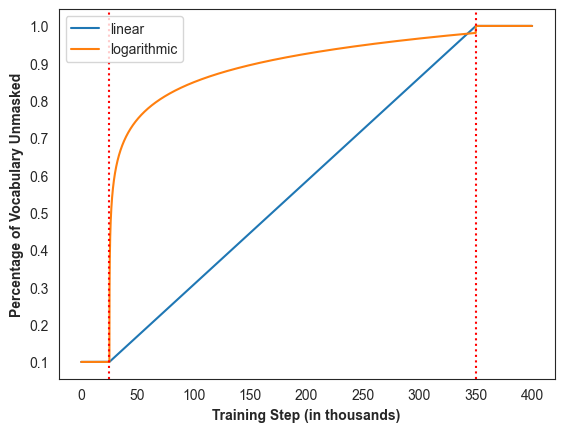
\includegraphics[width=0.45\textwidth]{chapters/climb/figures/pacing_fns.png}
    \caption{Illustration of the linear and logarithmic pacing functions used in my vocabulary curriculum experiments. The red dotted lines denote the curriculum regime, during which the percentage of unmasked words available to the model grows.}
    \label{fig:pacing_fn}
\end{wrapfigure}

Once a notion of difficulty is set, a pacing function is needed to govern how quickly the model will progress from training on easier examples to training on harder ones \citep{wu2021when}.

I experiment with two different pacing functions: linear and logarithmic. Linear pacing functions involve a steady and consistent advancement through the curriculum. This approach ensures a gradual increase in difficulty over time. Logarithmic pacing functions, on the other hand, emphasise early exposure to ``easier" concepts, with diminishing increments as the model's capabilities are assumed to increase. Both pacing functions have been proposed in the broader curriculum learning literature \citep{bai2022better, li2021curriculum, wu2021when}. In \cref{fig:pacing_fn}, I illustrate the two pacing functions for the vocabulary curriculum.

\begin{figure}[htbp]
    \centering
    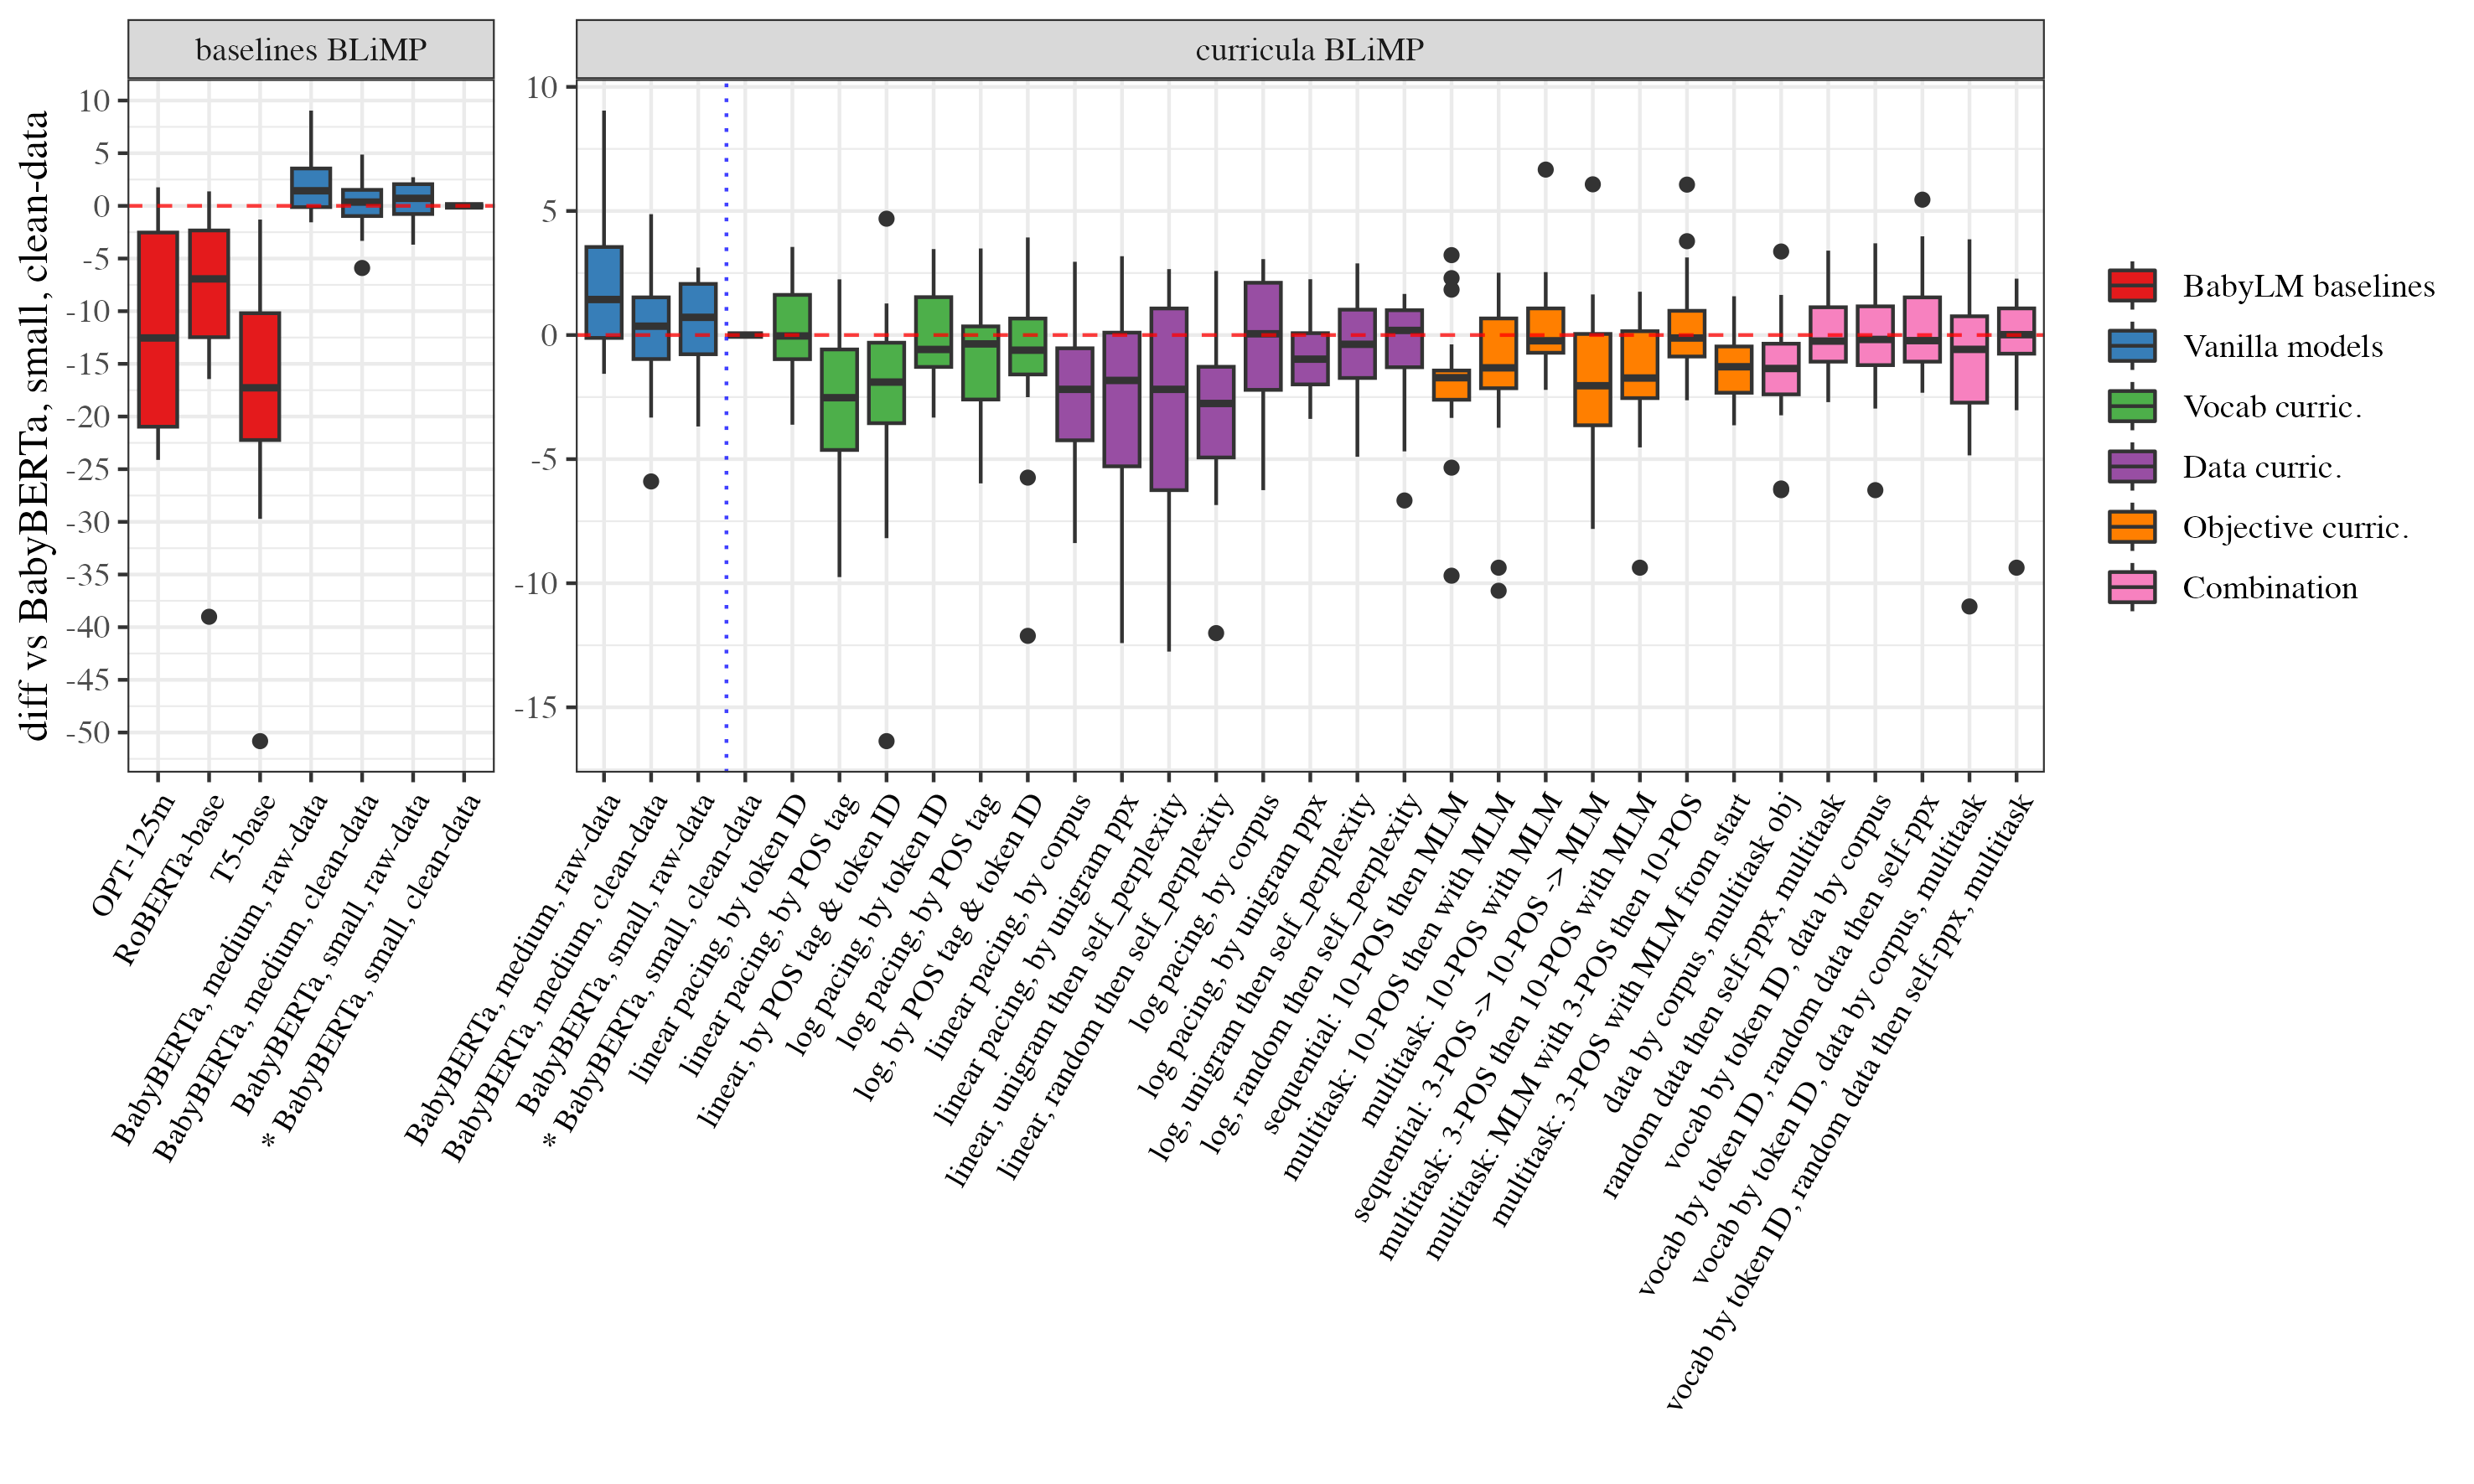
\includegraphics[width=0.9\textwidth]{chapters/climb/figures/babylm_blimp_diffs_boxplots.png}
    \vspace{1em}  % Add some vertical space between figures
    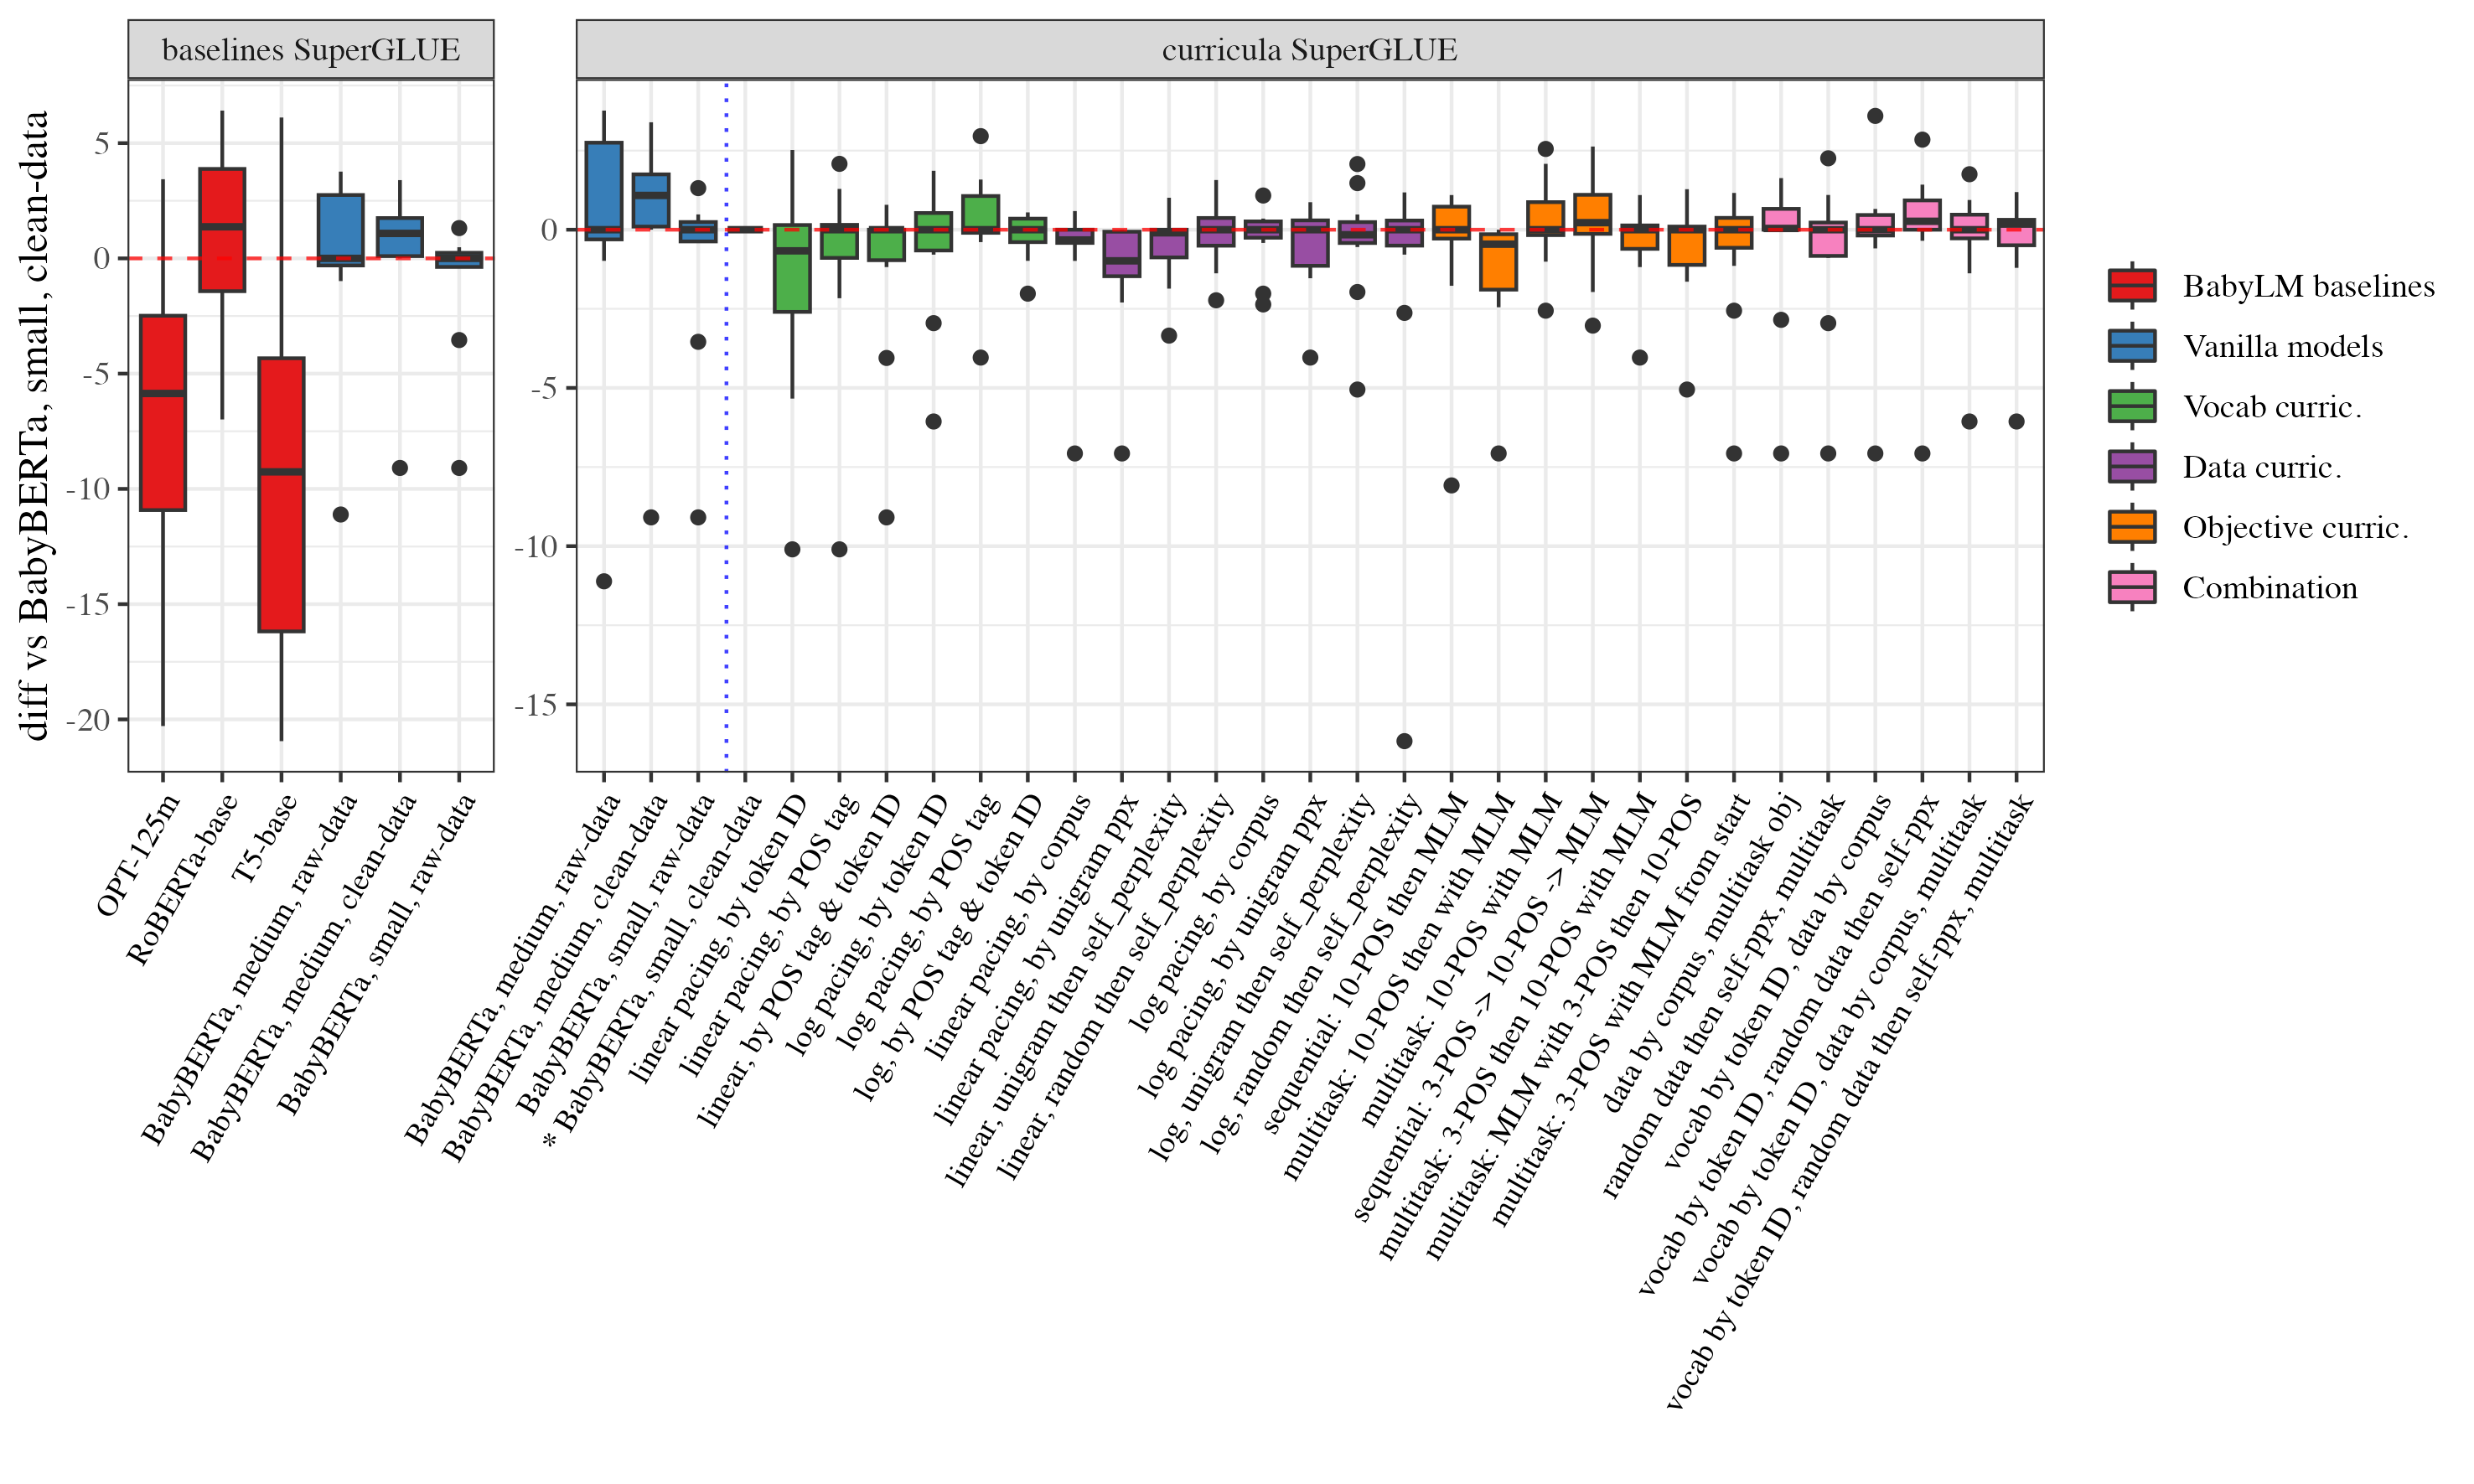
\includegraphics[width=0.9\textwidth]{chapters/climb/figures/babylm_superglue_diffs_boxplots.png}
    \caption{Comparison of model performance across BLiMP (top) and SuperGLUE (bottom) tasks. The plots show the differences in performance between the curriculum learning models and baseline models. Types of curriculum learning are indicated in the legend and highlighted with different colors with explanations in the text.}
    \label{fig:combined-boxplots}
\end{figure}


\section{Results}

Multiple evaluation metrics are employed in BabyLM. In this work, I focus on BLiMP \citep{warstadt2020blimp} and the supplementary BLiMP-style tests provided by the shared task organisers. I also report results on the natural language understanding benchmark, SuperGLUE \citep{wang2019superglue}, and the ambiguous subset of MSGS (the Mixed Signals Generalisation Set) \citep{warstadt2020msgs}. In brief, BLiMP evaluates specific linguistic abilities, MSGS evaluates linguistic preference over surface generalisation and SuperGLUE evaluates downstream task performance. For all scores, I report the average score across all categories, rather than test instances, as provided by the BabyLM evaluation pipeline.\footnote{For instance, there are 12 categories in BLiMP but 50+ individual tests. I average over the scores given for each category, rather than the scores given for each test.} All of the curriculum learning models are small BabyBERTa-style ones using the parameters shown in \cref{tbl:baseline-size-comparison} and the cleaned training dataset of 9.4M words (reduced from the 10M word dataset for the \textsc{strict-small} track). The results for each type of curricula are reported in separate Tables: \cref{tbl:result-vocab-cl} for the vocabulary curricula, \cref{tbl:result-data-cl} for data curricula and \cref{tbl:result-obj-cl} for objective curricula. Note that in each of these tables, I also provide the performance of the small BabyBERTa-style vanilla model that is trained on the same clean data as a baseline (\cref{subsec:baseline}). Additionally, \cref{fig:combined-boxplots} visualises a joint comparisons of all the curricula for the BLiMP and SuperGLUE tasks.

Furthermore, I experiemnt with combinations of different curricula to see how they would interact (\cref{tbl:result-combination-cl}). For all of my runs, I use the same set of hyper-parameters that I report in \cref{tbl:baseline_hyperparams}. 

I find notable gains for my own vanilla baseline models over the shared-task baselines, and, while I do not identify further large improvements in the curriculum learning models, I do notice some modest gains which suggest possibilities for future research and experimentation over variables. While the differences in performance between most of the experimental conditions are small, the large number of ablations provides a comprehensive set of recommendations for how and when different curriculum learning strategies may offer improved performance on linguistic tasks. Below I summarise my observations over the full results tables.

\begin{table*}
    \centering
    \small
    % \setlength{\tabcolsep}{3pt}  % Reduce column spacing further
    \begin{tabular}{ll|rrrrr}
    \toprule
    Pacing & Type & PPX & BLiMP & BLiMP.S & GLUE & MSGS \\
    \midrule
    Linear & \lightgreenhighlight{Freq} & 9.70 & 75.09 & \textbf{66.43} & 68.71 & 68.61 \\
    Linear & \darkgreenhighlight{POS} & 10.17 & 72.06 & 63.44 & 69.50 & 66.91 \\
    Linear & \verydarkgreenhighlight{Hybrid} & 10.21 & 73.37 & 66.11 & 69.22 & 66.61 \\
    Log & \lightgreenhighlight{Freq} & 9.26 & 74.97 & 64.63 & 69.94 & 66.82 \\
    Log & \darkgreenhighlight{POS} & 9.29 & 74.12 & 62.06 & \textbf{70.66} & \textbf{70.52} \\
    Log & \verydarkgreenhighlight{Hybrid} & 9.29 & 74.74 & 63.62 & 70.29 & 66.42 \\
    \midrule
    Vanilla & & \textbf{9.21} & \textbf{75.48} & 65.34 & 70.47 & 68.30 \\
    \bottomrule
    \end{tabular}
    \caption{\label{tbl:result-vocab-cl} Results for vocabulary curriculum models (\cref{subsec:vocab-cl}). All models score above 90 in the MSGS Control tasks. PPX = Perplexity, BLiMP.S = BLiMP.Supp, GLUE = (Super)GLUE, MSGS = MSGS Ambig.}
\end{table*}
    
I now summarise some key findings according to the three curriculum learning approaches: \textbf{vocabulary}, \textbf{data}, and \textbf{objective} curricula. As a general note, hile the curriculum models do not uniformly outperform the vanilla BabyBERTa-style baseline, I do observe small but consistent gains in some areas. These findings point toward useful strategies for future research on curriculum learning in low-resource language modelling.
\subsection{Vocabulary Curriculum}

\paragraph{Different representations of vocabulary difficulty work better for different tasks.}
When representing difficulty in the vocabulary curriculum experiments, token ID -- my proxy for frequency -- appears to work better than word classes (POS tags) or a combination of token ID and POS tags on the BLiMP evaluation tasks, but worse than POS tags on SuperGLUE and MSGS (\cref{tbl:result-vocab-cl}).

\paragraph{Log pacing sometimes helps for vocabulary curriculum learning, but not consistently.}
While log pacing outperforms linear pacing on BLiMP in 2 out of 3 configurations and across all SuperGLUE settings (3/3), it performs worse across the board on the BLiMP Supplement tasks (0/3). This suggests that pacing strategies for vocabulary exposure are task-sensitive. It is possible that the diverse vocabulary required by BLiMP Supplement tasks may not be well captured by the current pacing functions, indicating room for future exploration of more tailored schedules or functions inspired by non-monotonic learning trajectories.

\subsection{Data Curriculum}

\begin{table*}
    \centering
    \small
%    \setlength{\tabcolsep}{3pt}  % Reduce column spacing further
    \begin{tabular}{ll|rrrrr}
    \toprule
    Pacing & Type & PPX & BLiMP & BLiMP.S & GLUE & MSGS \\
    \midrule
    Linear & \lightpurplehighlight{Source} & 10.41 & 73.32 & 61.99 & 69.68 & 66.22 \\
    Linear & \darkpurplehighlight{Static PPX} & 12.51 & 72.45 & 61.67 & 69.10 & 66.90 \\
    Linear & \verydarkpurplehighlight{Dynamic PPX-U} & 11.88 & 72.62 & 62.57 & 69.86 & 66.64 \\
    Linear & \verydarkpurplehighlight{Dynamic PPX-R} & 10.82 & 71.88 & 63.10 & 70.37 & 67.48 \\
    Log & \lightpurplehighlight{Source} & \textbf{9.21} & \textbf{75.87} & 64.29 & 70.20 & \textbf{70.99} \\
    Log & \darkpurplehighlight{Static PPX} & 9.39 & 75.03 & 63.78 & 69.90 & 66.69 \\
    Log & \verydarkpurplehighlight{Dynamic PPX-U} & 9.35 & 74.83 & 64.24 & 70.09 & 66.89 \\
    Log & \verydarkpurplehighlight{Dynamic PPX-R} & \textbf{9.21} & 75.81 & 63.03 & 68.93 & 66.64 \\
    \midrule
    Vanilla & & \textbf{9.21} & 75.48 & \textbf{65.34} & \textbf{70.47} & 68.30 \\
    \bottomrule
    \end{tabular}
    \caption{\label{tbl:result-data-cl} Results for data curriculum models (\cref{subsec:data-cl}). All models score above 92 in the MSGS Control tasks. PPX = Perplexity, BLiMP.S = BLiMP.Supp, GLUE = (Super)GLUE, MSGS = MSGS Ambig.}
\end{table*}


\paragraph{In multi-corpora datasets, ordering by difficulty is a good first step.}
Training data requirements have grown so much in modern NLP that usually training a language model from scratch will involve multiple datasets, or multiple domains. The results of the data curriculum experiments indicate that a good first step is to put these sub-corpora into some order of intuitive difficulty, as I did (\cref{tbl:result-data-cl}). In the case of BLiMP this approach outperforms the perplexity-based data curricula, and with log pacing the vanilla model. The same is true of MSGS (with log pacing), as well as BLiMP-supplement and SuperGLUE (though the last two do not beat the vanilla model). 
Amongst the perplexity-driven models, the picture is less positive: out of 24 tests, only one model outperforms the vanilla model (log pacing, random initialisation + model perplexity in \cref{tbl:result-data-cl}).

\paragraph{Perplexity-driven approaches for data curriculum learning underperform.}
Although perplexity-based ordering intuitively reflects learning difficulty, it proves less effective in my experiments. Across 24 different perplexity-based configurations, only one outperformed the vanilla model (log pacing, random initialisation + model perplexity) \cref{fig:baseline_obj_cl_superglue}. This suggests that the perplexity estimates may not capture relevant complexity for the model at small scales, and further work is needed to refine how perplexity is computed or used.


\subsection{Objective Curriculum}
\begin{table*}
    \centering
    \small
    \begin{tabular}{l@{\hspace{-15pt}}lll|rrrrr}
    \toprule
    & \multicolumn{3}{l}{Task duration (\% of training)} & & & & \\
    Type & 3 POS & 10 POS & MLM & PPX & BLiMP & BLiMP.S & S.GLUE & MSGS \\
    \midrule
    \lightorangehighlight{Seq} & -- & 0 - 12.5 & 12.5 - 100 & 9.58  & 73.87 & 62.98      & 69.85       & 66.70    \\
    \darkorangehighlight{MT} & -- & 0 - 100 & 12.5 - 100 & 9.78   & 74.60 & 62.17     & 69.12       & 66.64    \\
    \darkorangehighlight{MT} & -- & 0 - 100 & 0 - 100    & 9.30  & \textbf{75.82} & 65.77     & \textbf{70.74}       & 66.58    \\
    \lightorangehighlight{Seq} & 0 - 6.25 & 6.25 - 12.5 & 12.5 - 100 & 9.49  & 74.03 & 63.02      & 70.71       & 66.93    \\
    \darkorangehighlight{MT} & 0 - 6.25 & 6.25 - 100  & 12.5 - 100 & 9.72  & 73.68 & 63.89     & 70.07       & 67.00    \\
    \darkorangehighlight{MT}  & 0 - 6.25 & 6.25 - 100  & 0 - 100    &  9.30 & 74.80 & \textbf{67.55}      & 69.89       & 67.65    \\
    \darkorangehighlight{MT} & 0 - 100  & -- & 0 - 100   & 9.25  & 74.48 & 63.98     & 69.77       & 67.72    \\
    \midrule
    Vanilla Model & &  & & \textbf{9.21}  & 75.48 & 65.34 & 70.47 & \textbf{68.30} \\
    \bottomrule
    \end{tabular}
    \caption{\label{tbl:result-obj-cl} Results for objective curriculum models (\cref{subsec:objective-cl}). All models score above 94 in the MSGS Control tasks. Task duration defines when an objective function was active during training, as a percentage of the total number of training steps.}
\end{table*}

\paragraph{Objective curricula, especially multitask setups combining POS tagging with MLM, show clear benefits on syntactic and downstream tasks.} \cref{fig:baseline_obj_cl_blimp_supp} and \cref{fig:baseline_obj_cl_superglue} compare the small BabyBERTa-style vanilla model to the best objective curriculum learning setting -- a multi-task trained model with sequential POS-tag prediction -- on each task in BLiMP Supplement and (Super)GLUE. I find that the curriculum-learning (CL) model outperforms the vanilla model on 5/6 tasks in BLiMP Supplement. While on (Super)GLUE, the CL model outperforms the baseline on 4/10 tasks and obtains comparable performance on another 4/10 tasks. This results illustrate the potential to further explore objective-curricula settings.


\begin{figure}[h]
    \centering
    \begin{subfigure}[b]{0.48\textwidth}
        \centering
        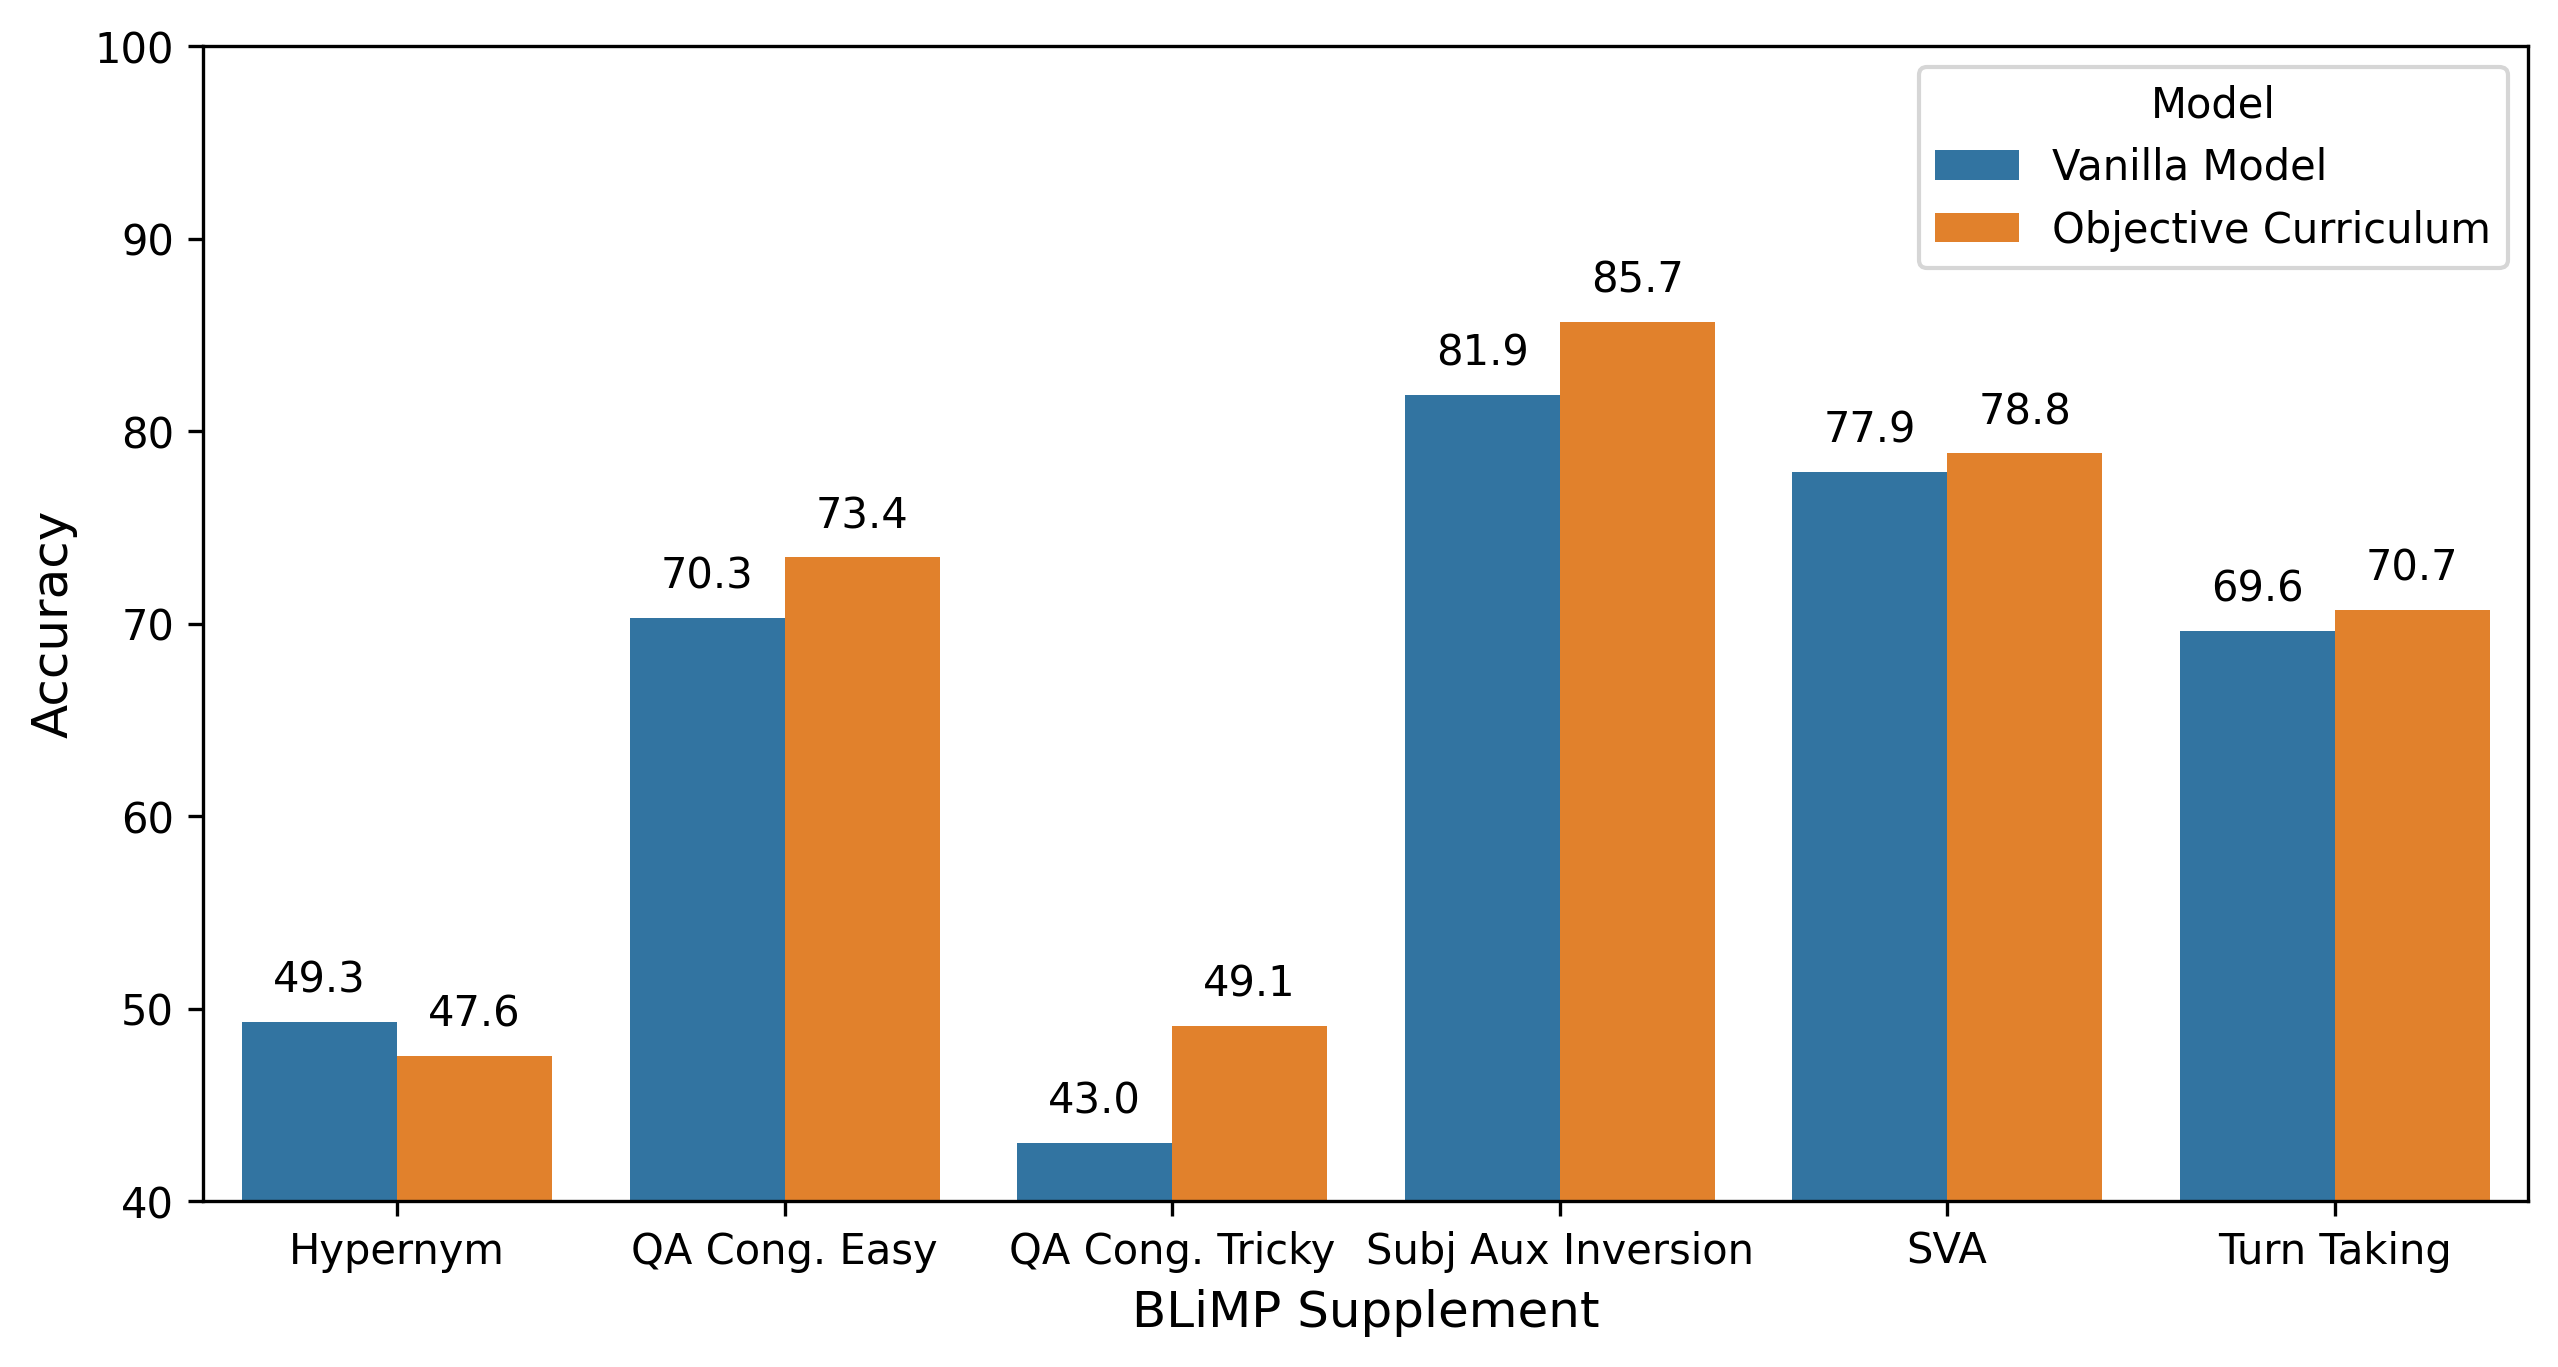
\includegraphics[width=\textwidth]{chapters/climb/figures/baseline_vs_obj_cl_blimp_supp_new.png}
        \caption{BLiMP supplementary tasks}
        \label{fig:baseline_obj_cl_blimp_supp}
    \end{subfigure}
    \hfill
    \begin{subfigure}[b]{0.48\textwidth}
        \centering
        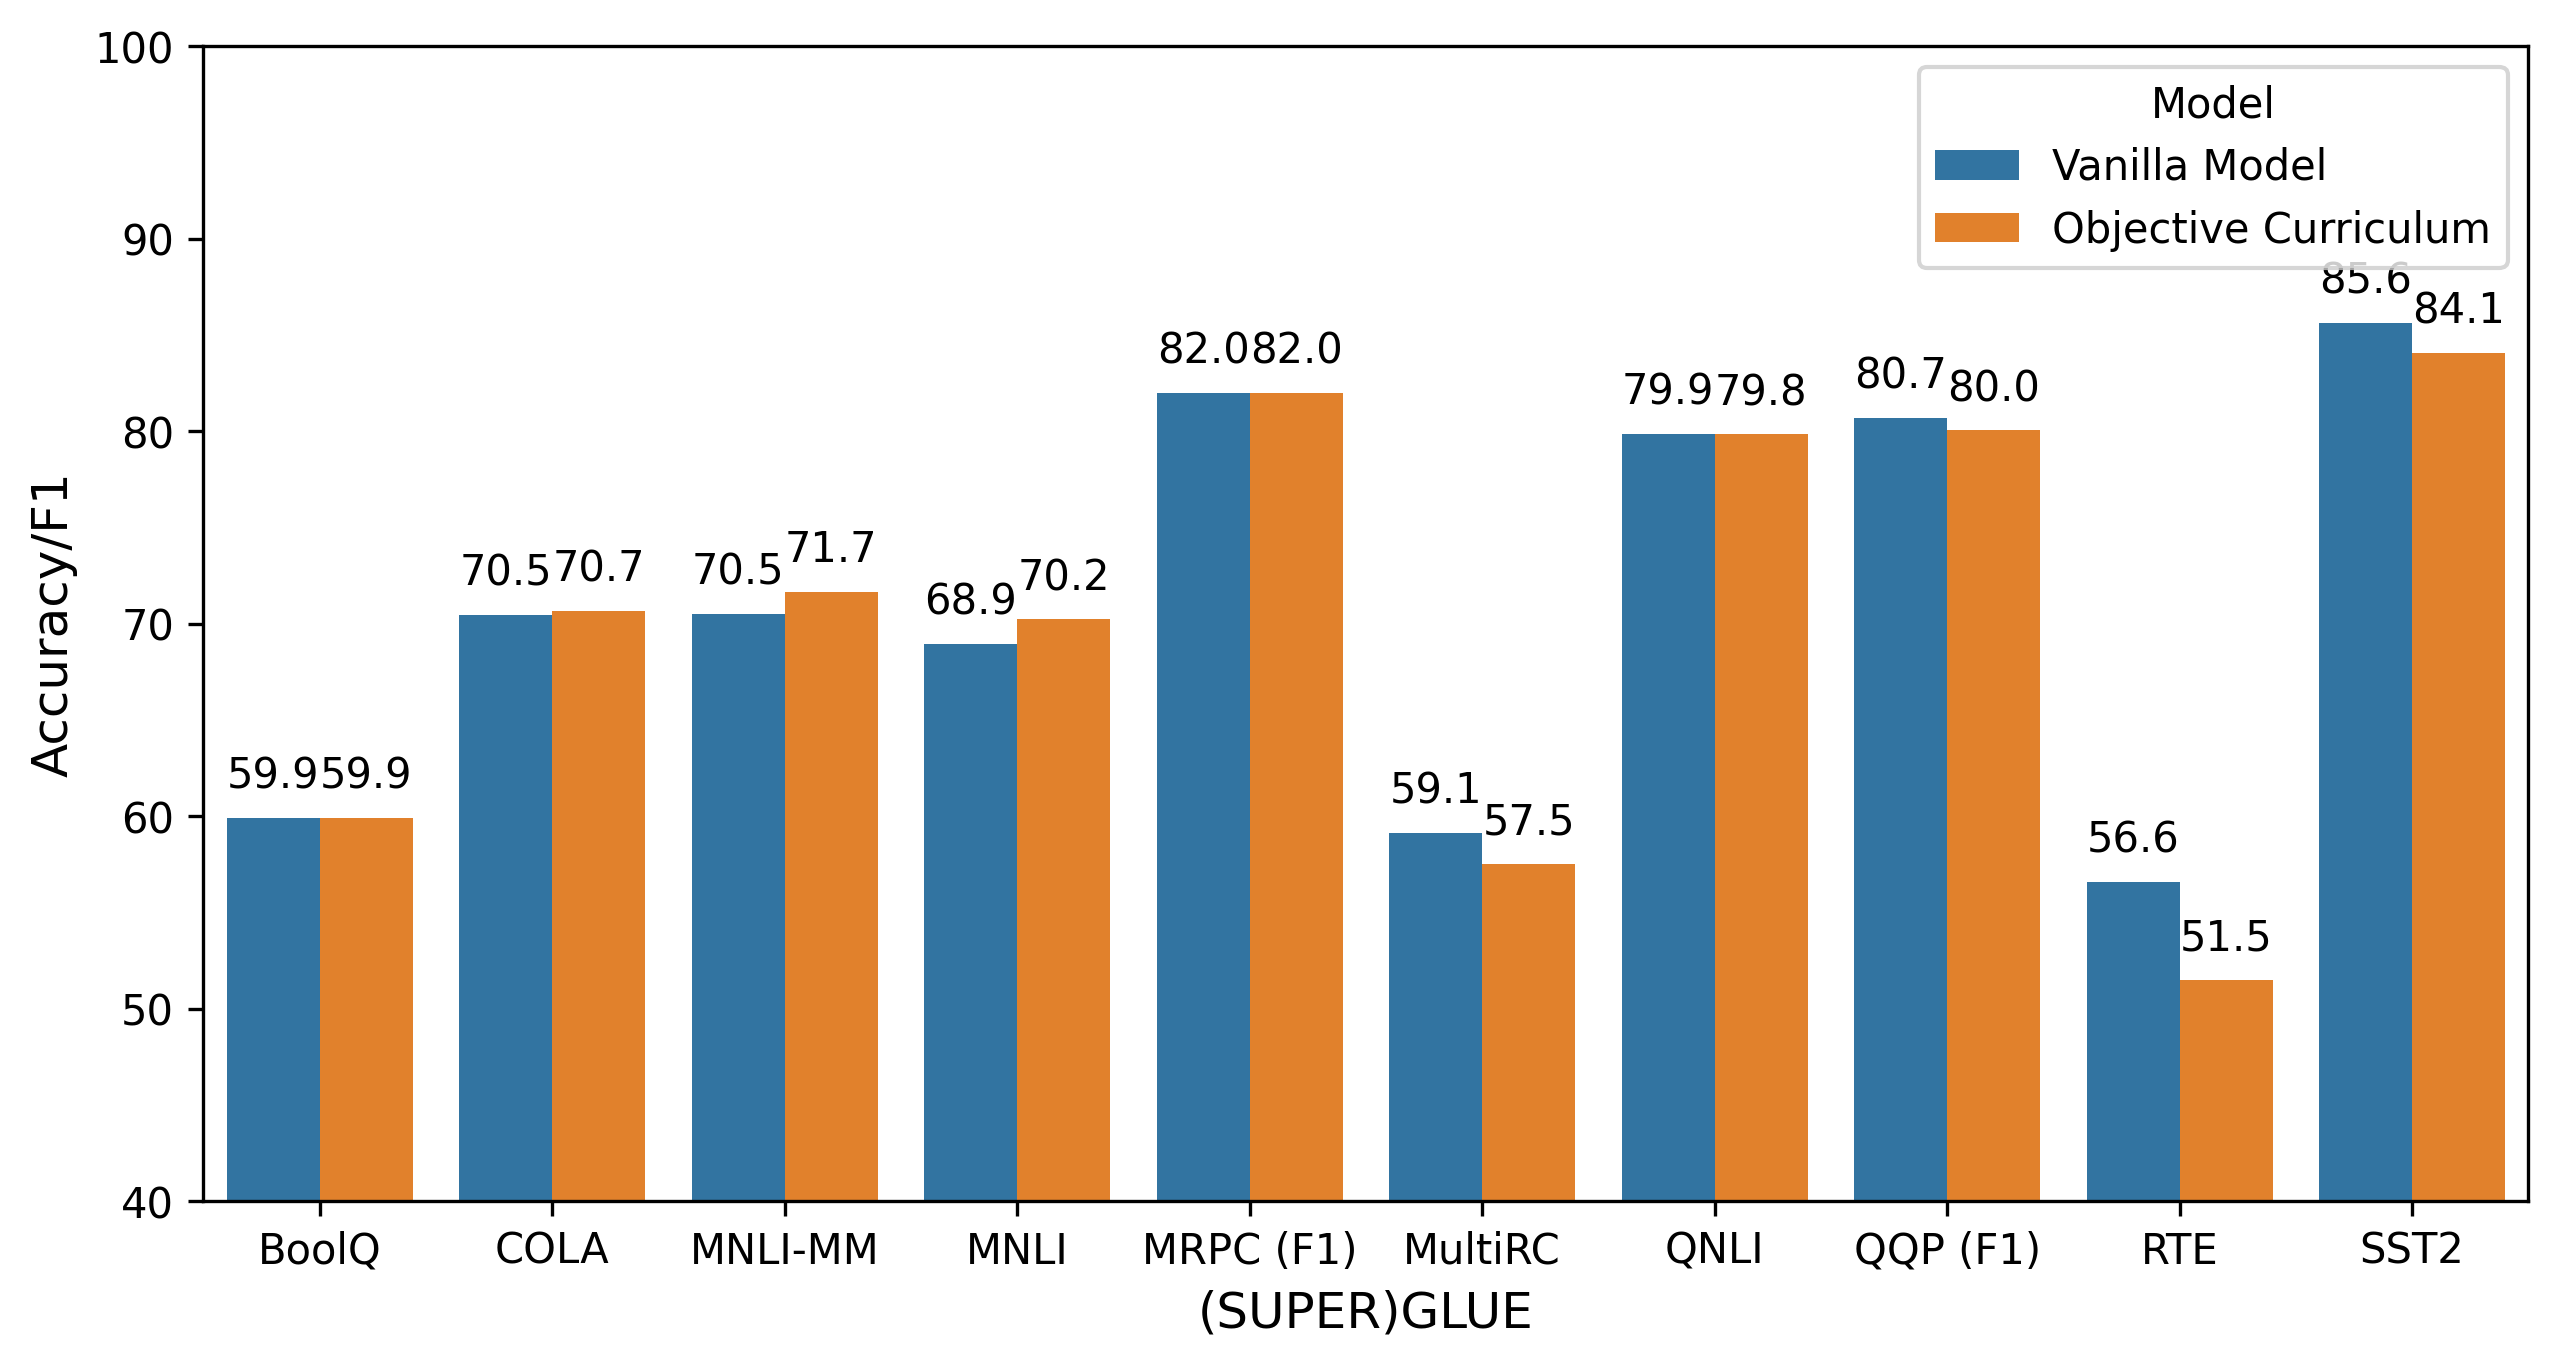
\includegraphics[width=\textwidth]{chapters/climb/figures/baseline_vs_obj_cl_superglue.png}
        \caption{(Super)GLUE tasks}
        \label{fig:baseline_obj_cl_superglue}
    \end{subfigure}
    \caption{Comparison between the vanilla model and the best objective curriculum learning setting on different benchmark tasks.}
    \label{fig:baseline_obj_cl_comparison}
    \end{figure}

I also experimented with curriculum learning via variation in training objectives. These include sequential curricula (where objectives are swapped at fixed training stages) and multitask learning setups (where multiple objectives are trained jointly).

\paragraph{Multitask learning holds sway over sequentially swapping objective functions for now.}
In the experiments with curricula for the objective function, I compare training on simultaneous tasks, known as multitask learning \citep{caruana1997multitask}, with predefined sequences of objective functions which swap from one to another at set thresholds in the training process. I set up two sequential curricula: one with 2 tasks (predicting the 10 universal POS tags found in the dataset, and MLM) and the other with 3 (like the 2 task curriculum, additionally with noun/verb/other prediction). I compare these against multitasking alternatives. In general the sequential curricula are outperformed by the multitasking ones, though the 3-task sequential curriculum outperforms the BabyBERTa-style vanilla model on SuperGLUE and is second only marginally to the best-performing multitask model (\cref{tbl:result-obj-cl}). The multitask learning model with 10-class universal POS-tag prediction and MLM in place from the outset performs best on BLiMP and SuperGLUE. However, the best model on BLiMP-supplement -- a multitask one -- has an element of sequential task scheduling in that the two POS-tag prediction tasks are lined up one after the other, with a switch from 3-class to 10-class after 6.25\% of training steps. In \cref{fig:baseline_obj_cl_blimp_supp}, I visualise this result for each task in BLiMP-supplement, illustrating that the curriculum learning model improves over the vanilla model in 5/6 tasks.

Altogether, these results suggest that sequential objective function curricula do hold some potential for performance gains if further tuning of the tasks and scheduling can be carried out.

\paragraph{Sequential training has potential with tuning.}
Although multitask learning tends to dominate, some sequential objective curricula also perform well. In particular, a 3-task curriculum (NOUN/VERB/OTHER POS prediction $\rightarrow$ 10-class POS $\rightarrow$ MLM) yields strong performance on SuperGLUE and is only narrowly behind the multitask version. These results indicate that sequential curricula may offer further benefits if task timing and transitions are more carefully optimised.

\paragraph{Objective structure aids syntactic generalisation.}
Models incorporating POS objectives (either in multitask or sequential form) often outperform vanilla models on BLiMP Supplement, which tests syntactic sensitivity. This supports the idea that structured auxiliary objectives guide the model toward syntactic generalisation, and could be explored further for syntactic evaluation tasks.

\subsection{Combined Curricula and Additional Observations}

\paragraph{In general, log pacing works at least as well as linear pacing across different curricula learning strategies.}
In the data curriculum experiments, models using the log pacing function outperform their linear counterparts in 4/4 settings on BLiMP, and 3/4 settings for BLiMP-supplement and SuperGLUE (\cref{tbl:result-data-cl}). This indicates that rapidly increasing the difficulty of training instances in the early stages brings downstream benefits on grammaticality and NLU tasks.

In the vocabulary curriculum experiments on the other hand, there is not such a clear picture. Log pacing outperforms linear in 2/3 settings on BLiMP and 3/3 on SuperGLUE, but 0/3 for BLiMP-supplement (\cref{tbl:result-vocab-cl}).
Presumably this is a reflection of the different vocabulary required by each set of evaluation tasks, which could be a matter for future investigation but also indicates that I do not yet have a clear generalisable pacing function for the vocabulary curriculum. There are of course other pacing functions to be tried.

\begin{table*}
    \centering
    \small
    \begin{tabular}{l@{\hspace{-10pt}}ll|rrrrr}
    \toprule
    Vocab \ & Data \ & Objective \ & PPX & BLiMP & BLiMP.S & S.GLUE & MSGS  \\
    \midrule
    -- & \lightpurplehighlight{Source} & \darkorangehighlight{MT} &                           9.29& 74.06 & 64.06 & 70.02 & 66.90 \\
    -- & \verydarkpurplehighlight{Dynamic PPX-R} & \darkorangehighlight{MT} &                9.44& 75.89 & 64.63 & 69.72 & 67.78 \\
    \lightgreenhighlight{Freq} & \lightpurplehighlight{Source} & -- &                     9.27& 75.89 & 64.62 & 70.24 & 67.90 \\
    \lightgreenhighlight{Freq} & \verydarkpurplehighlight{Dynamic PPX-R} & -- &        9.30& 75.88 & \textbf{65.79} & 70.42 & 66.63 \\
    \lightgreenhighlight{Freq} & \lightpurplehighlight{Source} & \darkorangehighlight{MT} &         9.22 & 74.86 & 62.82 & 70.09 & 66.68 \\
    \lightgreenhighlight{Freq} & \verydarkpurplehighlight{Dynamic PPX-R} & \darkorangehighlight{MT} & 9.46& \textbf{75.92} & 63.68 & 69.98 & \textbf{71.30} \\
    \midrule
    Vanilla Model & & & \textbf{9.21} & 75.48 & 65.34 & \textbf{70.47} & 68.30 \\
    \bottomrule
    \end{tabular}
    \caption{\label{tbl:result-combination-cl} Results for the combination curriculum models. The multitask objective curriculum refers to the 2-task 10-POS and MLM model shown in \cref{tbl:result-obj-cl}. }
\end{table*}

\paragraph{Combining all three curricula shows potential on BLiMP.}
While each individual curriculum learning experiment did not result in consistent improvements across tasks, I investigated whether combining aspects from the different curricula would, together, improve the model.
I do find that a combination of all three curricula outperforms any single curriculum model on BLiMP, but the same is not true for BLiMP-supplement and SuperGLUE (\cref{tbl:result-combination-cl}). This is another matter for future investigation, as it seems that improving each of the three curricula I investigate may lead to further gains if they are all combined.

\paragraph{In small data settings, filtering noisy data is in fact counter-productive.} Perhaps surprisingly, I find that the vanilla models trained on the raw data outperform those trained on the pre-processed data on BLiMP and MSGS. I surmise that models can learn even from linguistically non-standard datapoints.

\section{Discussion}\label{sec:discussion}

I set out to investigate a number of curriculum learning approaches to language model training, motivated by findings from the human language acquisition process and by the wish to successfully train smaller models for smaller budgets. I first of all implemented a stronger model of my own, based on BabyBERTa \citep{huebner2021babyberta} and found that a small 8-layer vanilla model could outperform the provided BabyLM baselines on the BLiMP grammaticality tests and get close to the best RoBERTa shared-task baseline on SuperGLUE. This underlines the findings reported in the BabyBERTa paper: that with smaller datasets, it makes sense to use smaller models and a smaller vocabulary size.

The results of the curriculum learning experiments, trained with a small BabyBERTa-style vanilla model, suggest that model performance can be improved in certain linguistic tasks by careful application of a pacing function, with certain types of curricula working more effectively than others. Specifically, I find that a logarithmic pacing function works better for the data curriculum than a linear one, but the findings for the vocabulary curriculum are less clear. Other pacing functions might be tried in the future, including those that reflect acquisition theory around non-monotonic or `U-shaped' development trajectories.

It is apparent that ordering the subcorpora within a training set may be worthwhile, and that perplexity-based approaches to data selection hold potential even though I have not found a clear-cut best method for perplexity calculation as yet. As shown in other NLP work, multitask learning can be a beneficial approach, though MLM or next-word prediction remain preeminent as singular tasks used in language modelling. I find multitask learning models hard to beat in the objective curriculum, but do find good performance in my sequential settings. I believe that future work varying the timing of task switches and introducing more tasks could be worthwhile.

On a more general note, the Baby LM challenge evaluates a language model only on its final downstream performance on a set of tasks -- i.e. at a finite point in time. The challenge does not directly measure whether a given model is learning in a `human-like' fashion. My contribution to the BabyLM challenge is to provide a set of curriculum learning strategies which are motivated by the language learning dynamics of infants and children. Future research could study how to quantitatively evaluate whether the learning trajectory of a model parallels that of a human language learner and how similarities to human language learning results in downstream NLU performance. 


\section{Conclusions}

This chapter explored how principles from child language acquisition can guide the structure and pacing of language model training. Specifically, I implemented three curriculum learning strategies inspired by human development: gradually increasing vocabulary size (\textbf{vocabulary curriculum}), ordering training data by intuitive or model-based difficulty (\textbf{data curriculum}), and varying the specificity of the objective function over time (\textbf{objective curriculum}).

Across these experiments, I found that the BabyBERTa-style vanilla models already outperform the BabyLM baselines on BLiMP and MSGS, and perform competitively on SuperGLUE. Curriculum learning approaches offer modest but consistent gains in some areas, particularly when using log pacing functions, source-based data ordering, or multitask objectives. These results suggest that developmental structure in training can yield benefits even in resource-constrained settings.

Notably, models trained on raw, unfiltered data often outperformed those trained on cleaned data, reinforcing the idea that early exposure to linguistic variation (even with noisy data) may help small models generalise better, much like children learning from diverse, real-world input.

Beyond specific gains, this chapter establishes a computational framework for implementing curriculum learning strategies aligned with cognitive development. In doing so, it addresses the macro-level question posed at the start of this thesis: \textit{can language models benefit from learning more like humans do, by following a structured, developmentally inspired trajectory?} 

The next chapter builds on this foundation by shifting focus to the micro-level dynamics of representation. There, I introduce \smoothing, a method motivated by how children use grammatical context to infer word meaning. While \climb explored how to structure the learning experience, \smoothing investigates how to shape internal representations to support better generalisation from limited exposure.


% \begin{table*}
% \centering
% \small
% \begin{tabular}{llrrrrr}
% \toprule
% Type              & Model    & PPX   & BLiMP & BLiMP.Supp & (Super)GLUE & MSGS Ambig \\
% \midrule
% Official Baseline & OPT-125m         & --    &   63.16 & 55.08 & 63.38 & 69.22 \\
%                   & RoBERTa-base      & --  &   
%                 69.84 & 50.52 & 71.42 & 70.25 \\
%                   & T5-base         & --    &   58.27 & 47.55  & 60.93 & 68.55 \\
% \midrule
% Vanilla Models    &CLIMB-base (medium)   & 9.01   & 75.66 & 66.13 & 70.75 & 67.62 \\
%                   & CLIMB-base-small & 9.21  & 75.48 & 65.34 & 70.47 & 68.30 \\
%                   & CLIMB-raw (medium)   &  8.47   & 77.97 & 66.16 & 70.63 & 69.44 \\
%                   & CLIMB-small-raw  & 8.64  & 76.42 & 64.60 & 69.46 & 70.65 \\
%                 & \emph{large-100M}      & 4.35      &   81.03 & 75.56 & 72.93 & 74.17 \\
% \midrule
% Vocab Curriculum          & CLIMB-tokens   &  9.70  & 75.09 & 66.43  & 68.71 & 68.61 \\
% Data Curriculum           & CLIMB-data-split & 9.21 & 75.87 & 64.29  & 70.20 & 70.99 \\
% Objective Curriculum      & CLIMB-multitask & 9.30 & 74.80 & 67.55  & 69.89 & 67.65 \\
% \bottomrule
% \end{tabular}
% \caption{\label{tbl:submission-comparison} Comparison between the official shared task baselines, our BabyBERTa-style vanilla models, and our submitted curriculum learning models on the main evaluation tasks: BLiMP, (Super)GLUE, and MSGS. Our *small and *medium models are defined in Section \ref{subsec:baseline}. All models are trained on pre-processed data except for those labelled with *-raw, which are trained on mostly unprocessed data (except we join the input sentences). The `large-100M' model was a larger BabyBERTa-style model trained on the 100M BabyLM training set (all others have been trained on the 10M dataset available in the \textsc{strict-small} track). }
% \end{table*}


% --- Additional Stuff ---

% \subsection{Curriculum Learning Approach}
% Our work introduces curriculum learning to three primary components of language model pre-training: vocabulary (Section \ref{subsec:vocab-cl}), data sampling approach (Section \ref{subsec:data-cl}), and objective function selection (Section \ref{subsec:objective-cl}). This multi-faceted approach is inspired by how humans learn language, where different aspects of language acquisition develop simultaneously but at different rates. For each component, we implement dynamic difficulty scaling that evolves over the course of training, simulating the progressive nature of human language learning. The specific variables and configurations for each curriculum learning experiment are detailed in Table~\ref{tbl:configurations}.

% \begin{table*}
%     \centering
%     \small
%     \begin{tabular}{llc}
%     \toprule
%          Type & Model & Training Time \\
%     \midrule
%          Vanilla Models & CLIMB-small-raw & 12h \\
%          & CLIMB-raw (medium) & 17h40m \\
%     \midrule
%          Data Curriculum & Log Source & 12h30m \\
%          & Log Random + model ppl & 17h10m \\
%          Objective Curriculum & Sequential All POS & 11h40m \\
%          & Multitask All POS & 15h30m \\
%          Vocabulary Curriculum & Linear POS & 11h50m \\
%          & Log Token ID & 12h10m \\
%     \midrule
%         Combination & Log Data Split + Log Token ID & 12h30m \\
%         & Log Random + model ppl + Log Token ID & 17h10m \\
%     \bottomrule
%     \end{tabular}
%     \caption{Compute required to train our models. We report the model with the shortest and longest runtime for each experiment type. Each model is trained for 400,000 steps with 4 A100 GPUs.}
%     \label{tbl:compute}
% \end{table*}

\chapter{Learning Words Like Humans Do: Syntactic Smoothing for Language Model Training}

While the Chapter 3 explored curriculum learning as a way to structure the input space and learning trajectory of a model, I now turn to a complementary question: \emph{how can internal representations themselves be shaped to better support generalisation—particularly for uncommon tokens?} Just as children benefit from structured exposure to language, they also rely heavily on syntactic cues to make sense of unfamiliar words. This chapter investigates how language models might likewise leverage structural signals to improve lexical generalisation.

One of the most striking capabilities of human learners is their ability to infer the meaning of unknown words from syntactic and semantic context; recall the example of the made-up word `zambled' from Chapter 2.

% Consider the sentence: ``the Golden Gate Bridge has been \emph{obnebulated} every morning this week, limiting visibility of the Pacific Ocean.'' Although most readers will not have encountered the word \textit{obnebulated}, we can make two confident inferences: (1) it is a verb, likely in the past participle form (given the ``has been'' auxiliary and the \textit{-ed} suffix), and (2) its meaning relates to fog or visibility. Human learners use this type of syntactic bootstrapping constantly.

This ability is notably lacking in current language models. Despite their success on many NLP benchmarks \citep{touvron2023llama, chowdhery2023palm}, pre-trained transformer language models still struggle with rare or unseen words. A key reason is that the vast majority of language models are pre-trained to maximise the log-likelihood of a word, given the surrounding context \citep{devlin2019bert, brown2020gpt3, chowdhery2023palm, touvron2023llama}. As language use is characterised by a Zipfian distribution \citep{zipf1935zipflaw}, language models are exposed to frequent tokens exponentially more often than infrequent ones during pre-training. Consequently, the representations of these frequent tokens are optimised based on exponentially more learning signals than those of low-frequency tokens. It has been shown that maximum likelihood objectives lead to representation degeneration in English language models because infrequent tokens are pushed into a narrow manifold of the representational space \citep{gao2018representation}. 

\begin{figure}[ht!]
    \centering
    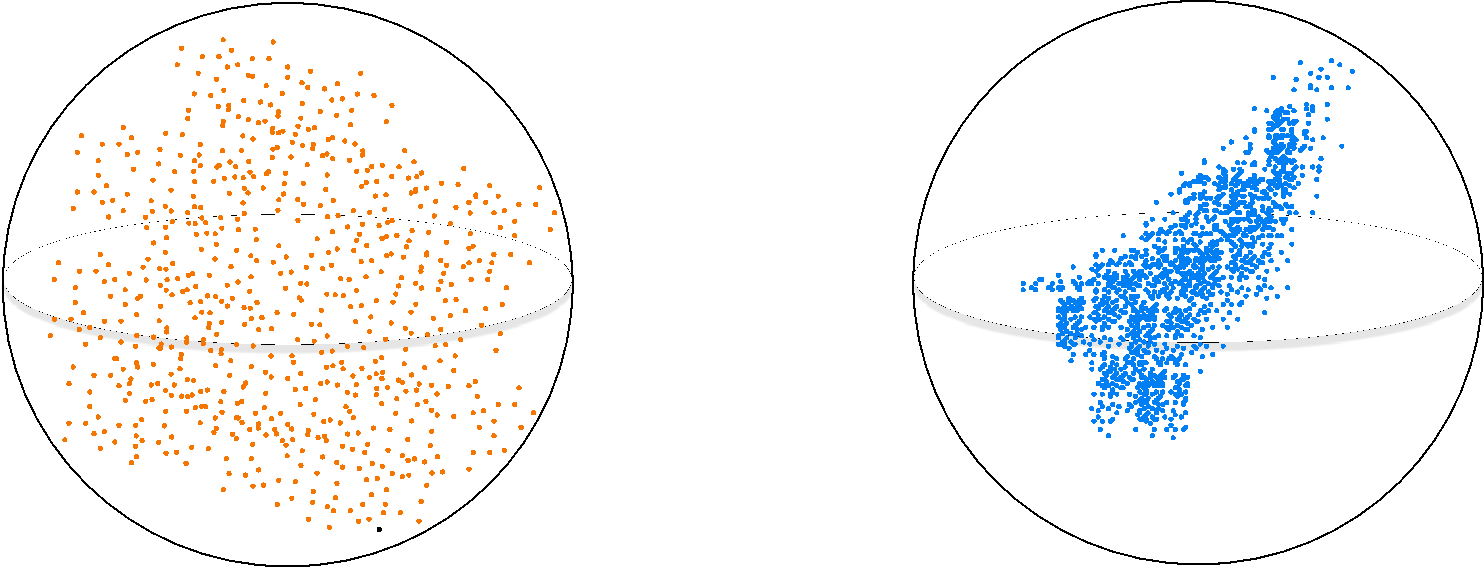
\includegraphics[width=0.8\linewidth]{chapters/syntatic-smoothing/figures/anisotropy_visualization.pdf}
    \caption{Artistic visualization of the representational space of a language model, showing the clustering of tokens into a narrow manifold. The model is trained with a maximum likelihood objective, and the representations of the tokens are clustered together into a narrow manifold.}
    \label{fig:anisotropy_visualization}
\end{figure}

\newpage

This representation degeneration problem is linked to the broader phenomenon of anisotropy: the hidden states of a language model tend to cluster together into a small cone-shaped subspace, rather than over their full representational capacity \citep{arora2016latent, ethayarajh2019contextual, gao2018representation}. \cref{fig:anisotropy_visualization} illustrates this phenomenon. As language model evaluation is based on cumulative evaluation scores that conceal how well a model processes infrequent words, the disparities in the representational space are difficult to assess. This work makes two key contributions:

\begin{enumerate}
    \item First, this chapter introduces \smoothing, a simple but cognitively motivated method for improving the representation of infrequent tokens during language model training.\footnote{The code for this chapter is available at: https://github.com/rdiehlmartinez/syntactic-smoothing.} Inspired by the human tendency to group unknown words with structurally similar known words, I propose redistributing part of the learning signal for each token across other tokens that share similar syntactic roles. Using this method, tokens that are seldom seen during training benefit from the more frequent updates of tokens that occur in similar syntactic functions.  In effect, infrequent tokens benefit from updates to their syntactic neighbors, allowing them to ``learn by association'', as children often do.
    \item Next, I quantify the impact of this approach using a new diagnostic measure of \textbf{frequency bias}: a model's tendency to prefer grammatical sentences that contain high-frequency tokens over those with low-frequency ones. I then show that \smoothing reduces both frequency bias and anisotropy, without hurting performance on downstream tasks. These findings suggest that small structural changes rooted in cognitive observations can meaningfully improve the robustness and generalisation of small models.
     
\end{enumerate}

The remainder of this chapter is organised as follows: \cref{sec:anisotropy-background} goes beyond the background chapter and reviews the relationship between frequency and anisotropy in language models. Building on this background, \cref{sec:freq-bias} introduces the frequency bias metric that I propose to quantify the degree to which a model relies on frequency information over linguistic generalisation. \cref{sec:smoothing-method} introduces the \smoothing method and details its implementation. \cref{sec:results} both presents the results and analysis across synthetic and real-world evaluations and discusses the implications of these findings. Finally, \cref{sec:conclusion} summarises this work and motivates further exploration of how language models internalise linguistic structure over time.

\section{Anistropy}
\label{sec:anisotropy-background}


Through maximum likelihood training, language models implicitly learn to encode token frequency statistics. This training process gives rise to a frequency bias in models that constrains their ability to generalise to infrequent tokens. In this chapter, I will describe how this training process leads to a phenomenon known as anisotropy in language models' representational space. Before doing so, in this section, I describe more concretely how anisotropy is defined and how it is measured.

% \subsection{Generalization to Infrequent Tokens}

% Current approaches to language modeling rely heavily on the memorisation of infrequent tokens to perform well on downstream tasks \citep{feldman2020does}. Recent analytical work has shown that certain layers of transformer models implicitly store memorised long-tail data \citep{haviv2023understanding, kobayashi2023transformer}. \citet{feldman2020neural} demonstrate that models memorise atypical examples to achieve the highest accuracy on long-tailed data samples. This memorisation hack, however, has only been shown to work well with over-parameterised models \citep{belkin2019reconciling}. While these studies present various metrics to evaluate memorisation, these metrics do not capture how memorisation impacts generalised linguistic understanding within the models. In our work, we address this gap by developing a metric that quantifies the extent of this frequency bias in relation to models' linguistic abilities.

% Language use follows a Zipfian distribution, meaning that many tokens appear infrequently. Standard training objectives often require large models and noisy datasets with sufficient long-tail samples for effective generalisation \citep{zheng2022memorization}. However, improving generalisation without excessive scaling can be achieved by training models with inductive priors that leverage linguistic information. On the lexical level, the integration of morphological and orthographic information during representation learning has been explored to obtain more fine-grained word embeddings \citep{salle2018incorporating, vulic2017morphfitting, cotterel2015morphological, bhatia2016morphological, botha2014compositional}. To improve syntactic generalisation, the objective function has been enriched with auxiliary tasks, such as predicting constituency labels \citep{wang2023language}, hypernyms \citep{bai2022better}, dependency tags \citep{cui2022lert}, and POS tags \citep{diehlmartinez2023climb}. Some approaches have also shown promising results on rare word performance by constructing token embeddings that consider a word's surface form and surrounding context \citep{schick2019attentive, schick2020rare}.

\subsection{Anisotropy in Representational Space}
While frequency bias and generalisation capabilities can be observed by analysing model behavior on input--output patterns, representational analyses indicate that these phenomena are linked to the distribution of token representations. Language models trained as likelihood maximisers have been shown to yield degenerate representations for rare tokens \citep{gao2018representation}. Throughout training, infrequent tokens are disproportionately pushed in the negative direction of most hidden states, resulting in their clustering together irrespective of their semantic or syntactic properties. This clustering behavior leads to anisotropy: rather than occupying a large region of the representational space, token representations lie along a narrow manifold \citep{gao2018representation, ethayarajh2019contextual}

\subsection{Defining Anisotropy}

Anisotropy is defined as the inverse of isotropy: $1-I(v(\cdot))$. A representational space is isotropic if all the vector directions are distributed uniformly, meaning no particular direction is favored over another.

\citet{arora2016latent}\ and \citet{mu2018all} define isotropy as:

\begin{equation}
    I(v(\cdot)) \coloneq \frac{\min_{\norm{c}=1} Z(c)}{\max_{\norm{c}=1} Z(c)}
\end{equation}
where $c$ is a unit vector and $Z(c)$ is defined as the partition function over all tokens $w$ in the vocabulary $V$ , with representations $v(w)$:
$$
    Z(c) = \sum_{w \in V} \exp(c^Tv(w))
$$
In practice, this definition of isotropy is analytically infeasible to solve. In this chapter, I follow an empirical approximation proposed by \citet{ethayarajh2019contextual}: 
\begin{equation}
\label{eq:empirical-isotropy}
    I(v(\cdot)) \coloneq \mathbb{E}_{i\ne j}\big(1-\cos(v(w_i), v(w_j))\big)
\end{equation}
Here, $w_i$ and $w_j$ are two tokens sampled from the vocabulary, and $\cos$ is defined as taking the cosine similarity of the two word representations for $w_i$ and $w_j$.  

Despite its prevalence, the impact of anisotropy on a model's language understanding abilities remains unclear. Some studies suggest that reducing anisotropy improves performance on non-contextual benchmarks, sentence comparison tasks, and multilingual benchmarks \citep{bis2021too, su2021whitening, rajaee2022isotropy}. Conversely, other research indicates that higher anisotropy might enhance semantic clustering tasks and that reducing anisotropy does not uniformly improve performance on common NLU tasks \citep{ait2023anisotropy, ding2022isotropy}. Furthermore, the relationship between anisotropy and maximum likelihood training has been questioned. Some researchers argue that isotropy exists in local manifolds of contextual word representations \citep{cai2020isotropy}, while others contend that anisotropy arises from the learning dynamics of the query and key attention matrices in transformer models \citep{godey2024anisotropy}.

% \subsection{Reducing Anisotropy}

% Existing methods to reduce anisotropy broadly fall into three categories. The first group of approaches transforms the hidden states of language models to remove semantically uninformative directions and to preserve the dimensions of maximal isotropy \citep{arora2016simple, mu2018all, raunak2019effective, su2021whitening,bis2021too}. This intervention style is based on the assumption that the top singular dimensions of pre-trained word representations encode frequency statistics rather than semantic or lexical information \citep{mu2018all}. The second category of methods introduces novel training objectives and regularization terms that reduce the effects of anisotropy \citep{gong2018frage, gao2018representation, wang2019improving}. This type of approach places an inductive bias on representations that push the embeddings of frequent and infrequent words to occupy a similar semantic space. The third set of approaches explores different training paradigms to directly minimise anisotropy, such as using normalizing flow models \citep{li2020sentence} or manipulating the gradients used in maximum likelihood models \citep{yu2022rare}.

\vspace{1em}

While frequency bias and anisotropy are prevalent in language modeling, quantifying their effects and understanding their impact on generalisation, particularly for infrequent words, remains an open area of research. This chapter introduces a novel method for improving the representation of infrequent tokens by integrating linguistic information. Moreover, I hypothesise that adjusting the learning process to better represent infrequent tokens will also reduce anisotropy, as these two phenomena are interconnected.

\section{Frequency Bias}
\label{sec:freq-bias}

BLiMP is carefully balanced to ensure individual tokens occur equally in both sentence types. However, within a single pair, there may be an imbalance in average token frequency: For instance, the sentence
\textit{Grace's piano teachers are \textbf{known}} has a log frequency of 8.35 while its associated minimal pair \textit{Grace's piano teachers are \textbf{replied}} has a log frequency of 6.20.  I hypothesise that despite the minimal difference in BLiMP pairs, models trained in a typical manner will be biased by token frequency when determining grammatical acceptability.

\begin{wrapfigure}{r}{0.6\textwidth}
    \centering
    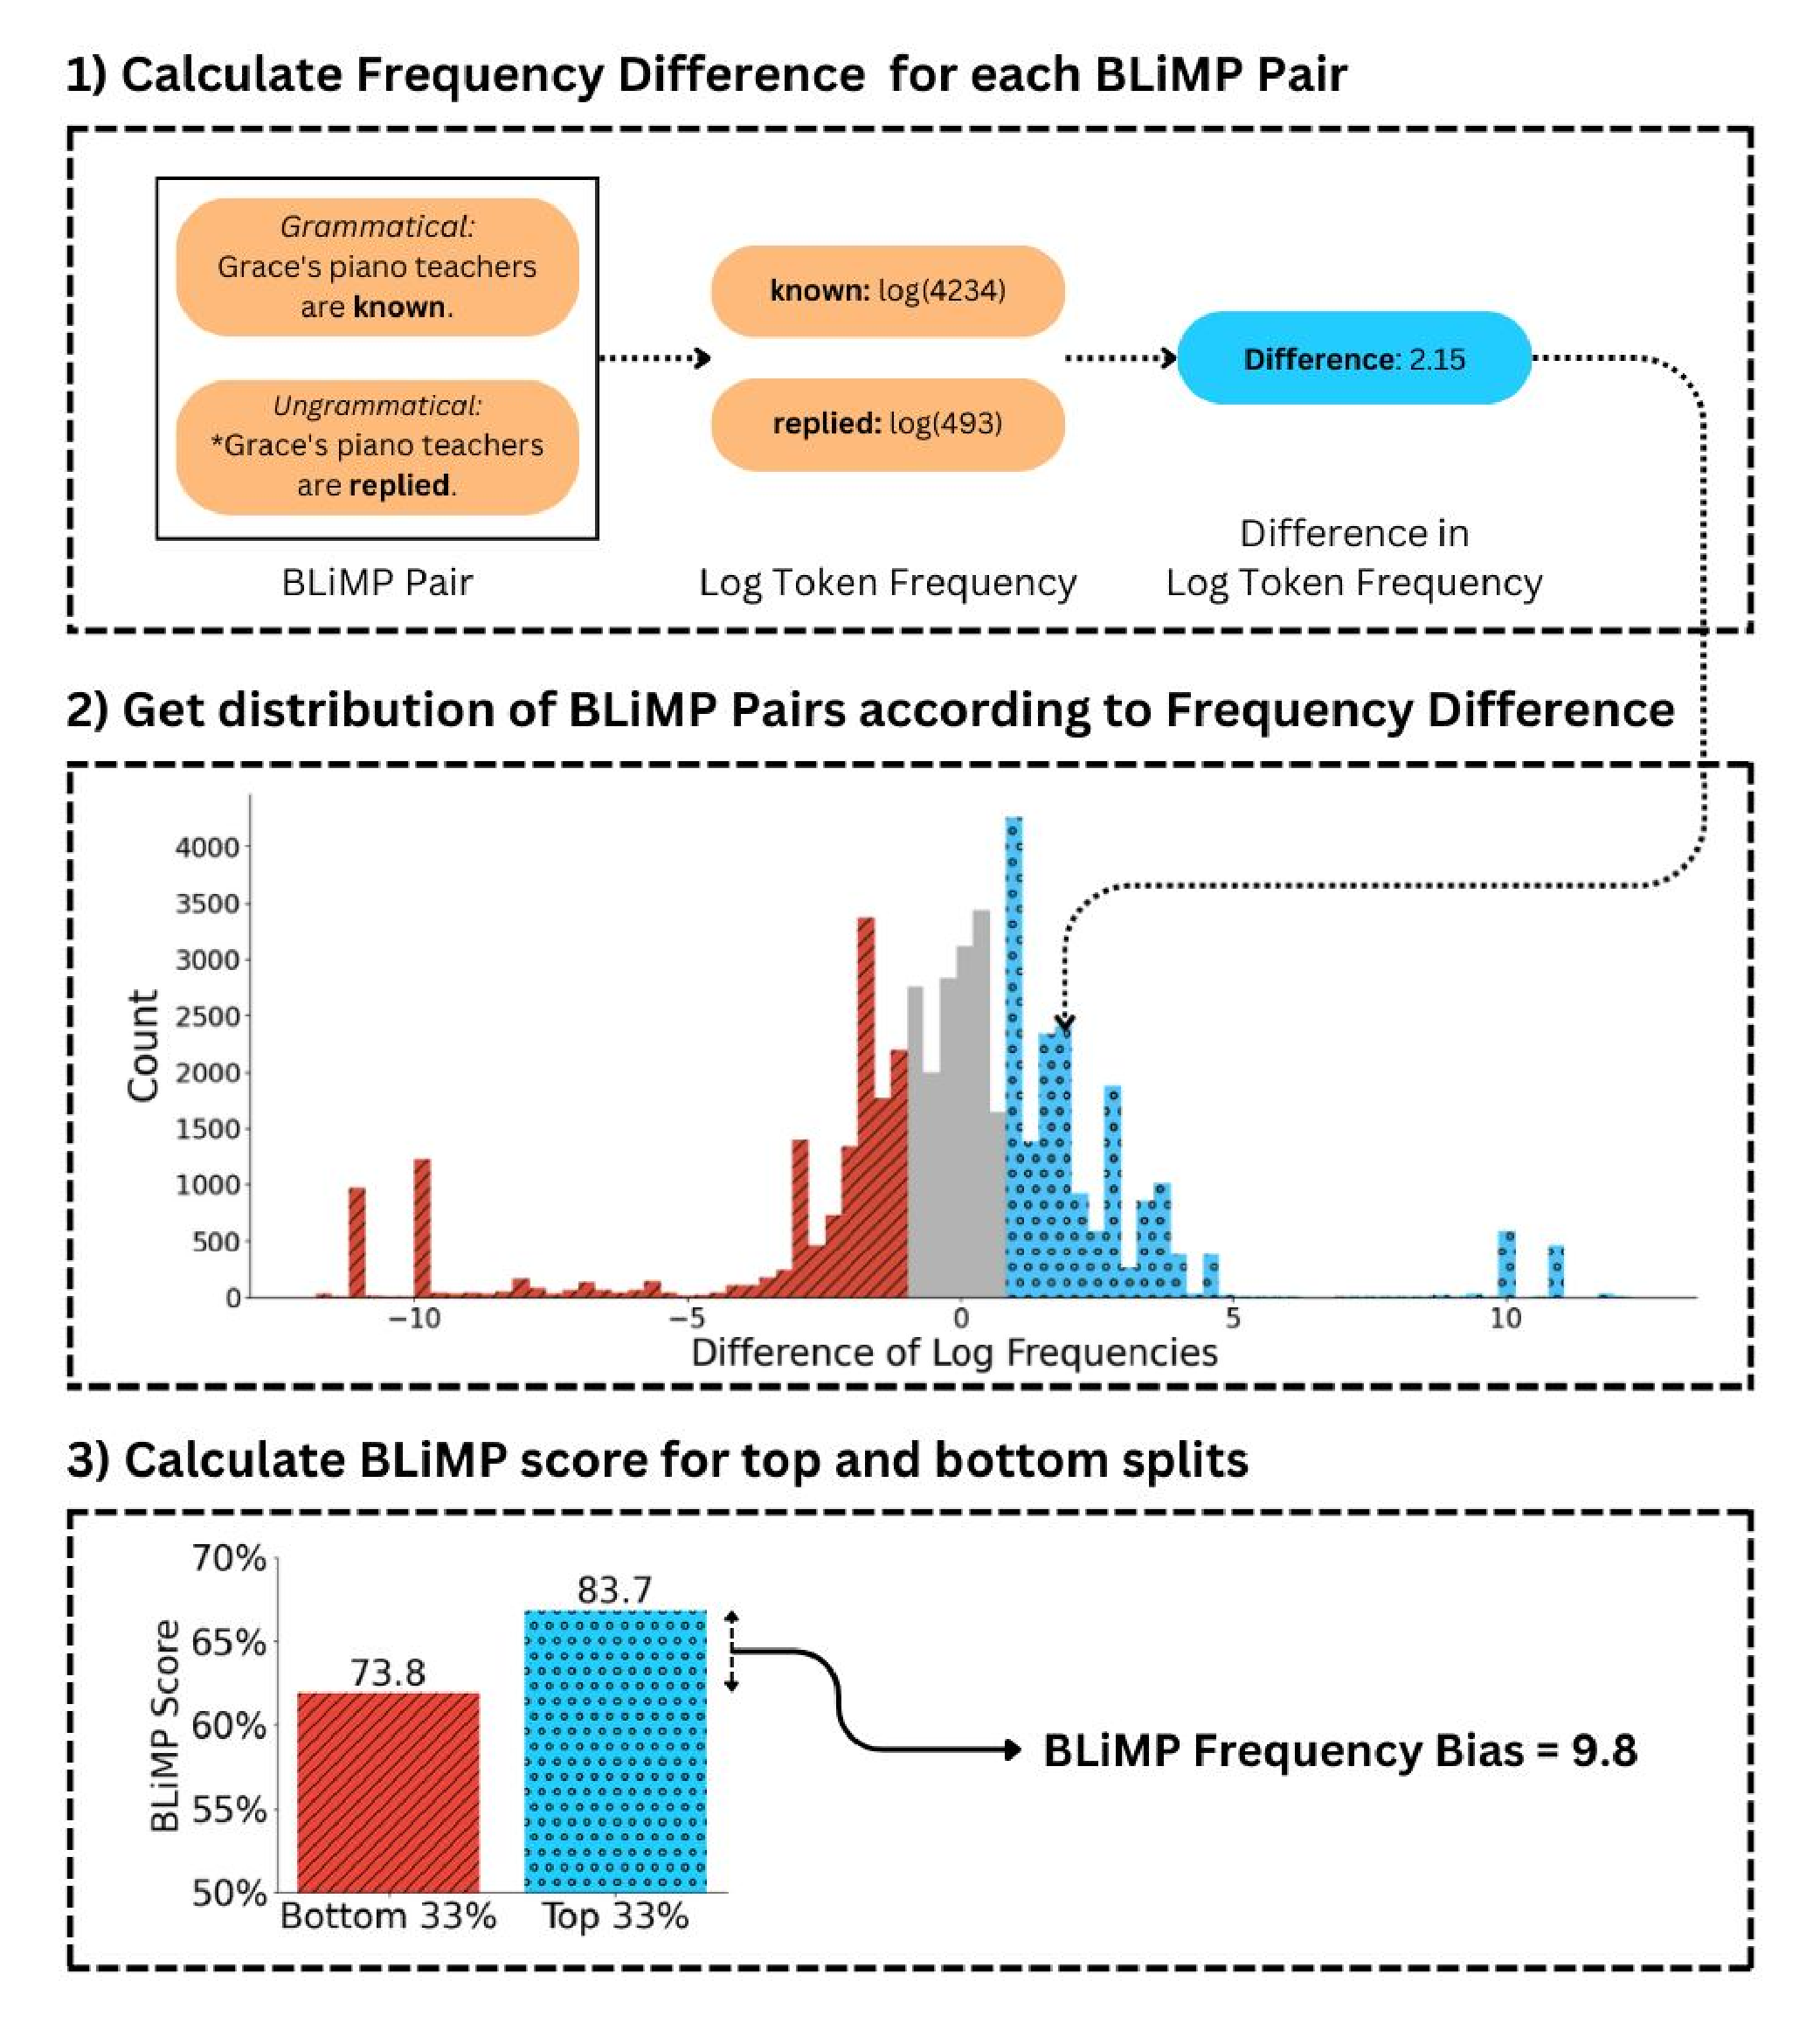
\includegraphics[width=0.6\textwidth]{chapters/syntatic-smoothing/figures/blimp_bias_example.pdf}
    \caption{Illustration of the BLiMP \textbf{frequency bias} calculation used to evaluate a model's reliance on frequency statistics when making predictions. The example BLiMP values are from a baseline RoBERTa model.}
    \label{fig:blimp_bias}
    \vspace{-1em}
\end{wrapfigure}

My goal is to quantify how language model performance differs between BLIMP pairs with large positive frequency differences (where the correct sentence has more frequently occurring tokens) and with large negative frequency differences (where the correct sentence has much less frequently occurring tokens). I do so in three steps.

First, I minimally preprocess BLiMP to ensure the analysis focuses on meaningful token-level differences. Specifically, I filter the dataset to only include sentence pairs where one set of tokens has been replaced by another set (e.g., ``The cat sat" vs ``The dog sat"). I exclude sentence pairs that differ only in token order (e.g., ``The cat sat" vs ``Sat the cat") or where tokens have been added to one sentence but not replaced (e.g., ``The cat sat" vs ``The cat sat quietly"). This filtering process removes approximately 15\% of the original BLiMP pairs and 9 of the 67 linguistic subtasks from consideration, but ensures that the frequency bias analysis focuses on genuine token-level substitutions that are most relevant for studying lexical generalisation.

Next, for each BLIMP sentence pair, I calculate the average (natural log) frequency of the differing tokens. Frequencies of individual tokens are computed with respect to a model's training data; for instance, in the example above the token \textit{\textbf{known}} has a log frequency of 8.35 in the training data. Sentence pairs are then ranked by the relative difference in these average frequencies, where positive values indicate a higher average frequency for the acceptable sentence. These relative differences form a distribution, as shown in the middle plot of \cref{fig:blimp_bias}. 

Then, I compute the BLiMP score using pseudo log-likelihood \citep{salazar2020masked} for BLIMP pairs in the upper and lower thirds of the relative frequency difference distribution. I exclude the middle third, as these represent pairs with minimal frequency differences (see the frequency plot for details). I define a model's \textbf{frequency bias} as the difference between the two BLiMP scores. The entire process is illustrated in \cref{fig:blimp_bias}. While the choice of partitioning the frequency pairs into thirds is somewhat arbitrary, I find that this division works well empirically; expanding the middle set of BLIMP sentences that I exclude would make the \textbf{frequency bias} more pronounced, but would lead to data sparsity. 

In practice, I find that standard transformer language models, such as OPT-125M \citep{zhang2022opt}, RoBERTa-base \citep{liu2019roberta}, and T5-base \citep{raffel2020t5}, exhibit a frequency bias as high as 13.7\%. My goal is to develop a model that can attain a frequency bias close to zero while attaining a high BLiMP score: that is, a model that makes determinations on the grammatical acceptability of sentences based solely on relevant linguistic aspects, rather than relying on possibly misleading statistical artifacts of the training data. 

\section{Syntactic Smoothing}
\label{sec:smoothing-method}

I hypothesise that transformer language models exhibit a strong frequency bias due to their maximum likelihood training objective, which limits infrequent tokens from receiving useful learning signals and thus hinders their ability to effectively encode linguistic information. To address this, I propose at each learning step to backpropagate the learning signal of a target token to all other tokens serving similar syntactic roles; this benefits infrequent tokens that appear less often in the training data.

\smoothing implements this strategy by distributing a portion of every update signal to all syntactically similar tokens using a syntactic similarity metric (operationalised below). This results in the representation of infrequent tokens approaching the average representation of all tokens that serve a similar syntactic function; e.g., the representation of a niche word like `obnebulated' would encode its syntactic role as a verb.

The \smoothing method consists of two components; (1) a similarity metric that uses part-of-speech distributions as a coarse proxy for syntactic similarity, and (2) an adjustment to the loss function to smooth the backpropagation signal over syntactically similar tokens during pre-training. 

\subsection{Syntactic Similarity Score}\label{sec:sim}

The syntactic similarity between two tokens can be measured in multiple ways, e.g., by using surface features, dependency labels, or even the predictions of a teacher language model \citep{hinton2015distilling}. Here, I present a simple measure that acts as a coarse approximation for syntactic similarity: I consider two tokens to be similar if they have a similar distribution of part-of-speech tags in the training set.

I evaluate the syntactic similarity between tokens prior to training, as a one-off preprocessing step over the entire training set. First, I use the part-of-speech (POS) tagger from the NLTK package \citep{bird2009natural} to assign each word in the training set to one of 12 universal POS tags, based on its given context \citep{petrov2012universalpos}.\footnote{The 12 tags in the NLTK tagger are given here: \url{https://www.nltk.org/book/ch05.html\#tab-universal-tagset}. They are derived from the 17 tags in the Universal Dependencies tagset.} I then tokenise the training data into sub-word tokens and assign each token the POS tag corresponding to the word it belongs to in each instance. As words can take on a different part of speech depending on the context, I count the number of times each token in the vocabulary $V$ appears as each POS tag in the training data, producing a 12-valued vector. This results in a matrix $M \in \mathbb{R}^{|V|\times 12}$ containing the distribution over POS tags for each token. Finally, I can compute the similarity of two tokens $V_i$ and $V_j$ using the cosine similarity of their POS distributions: $$ \text{Syntactic Similarity(i, j)} = \frac{M_i^TM_j}{||M_i|| \cdot ||M_j||}$$ 


Note that while in this chapter I define syntactic similarity via cosine similarity, any real-valued distance metric or divergence can be used. The similarity function does not need to be symmetric, although I note that symmetric functions provide computational advantages as only half the values need to be computed and stored. Also, note that this methodology does not depend on a specific choice of POS tagger.

I provide the POS distributions and similarity distributions for the example tokens ``blind'' and ``the'' in \cref{fig:distributions}. Notice that ``the'' occurs almost exclusively as a determiner and is not similar to many other tokens, whereas ``blind'' occurs as a noun, verb, adjective, and adverb and has a high similarity to more than half the other tokens in the vocabulary.

\begin{figure}[ht!]
    \centering
    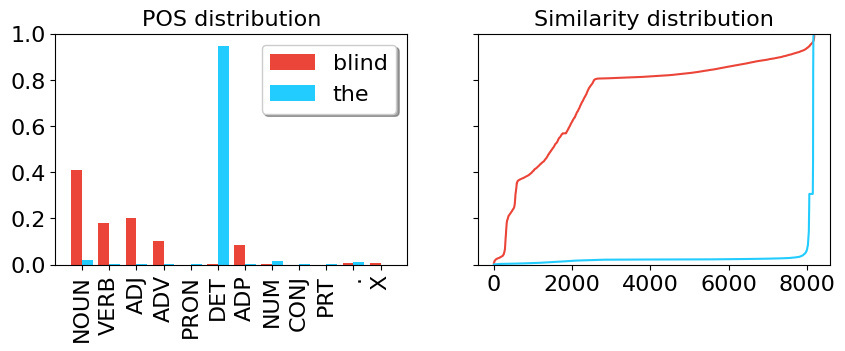
\includegraphics[width=0.8\linewidth]{chapters/syntatic-smoothing/figures/distributions.png}
    \caption{Part-of-speech distributions and similarity distributions for the subword tokens ``blind'' and ``the''. Similarities are computed as cosine-similarities against every other token in the vocabulary and sorted.}
    \label{fig:distributions}
    \vspace{-1em}
\end{figure}

\subsection{Smoothing the Backpropagation Signal}\label{section:smoothing}

Modern pre-training objectives implement likelihood maximisation using a cross-entropy loss between the label of the correct word and predicted probabilities from a forward pass of the model. \smoothing makes a small adjustment. Instead of a one-hot encoding, the target vector $t$ becomes a distribution across the entire vocabulary with some of the signal on the correct label $j$ and the rest of the signal distributed across all other tokens $i$ according to the syntactic similarity metric used:

\begin{equation}
\label{eq:signal-distribution}
    t_i=\left\{
  \begin{array}{@{}ll@{}}
    (1-\alpha), & \text{if}\ i=j \\
    \frac{s(i,j)}{\sum_{k=0}^{|V|}{s(i,k)}} \times \alpha & \text{otherwise}
  \end{array}\right.
\end{equation}

\noindent

where $\alpha$, the smoothing parameter, determines the proportion of the error signal reserved for the correct word and $s$ is the part-of-speech similarity metric. I experiment with different values for $\alpha$, noting that $\alpha=0$ is the standard likelihood maximisation task. I also investigate the use of a pacing function that linearly decreases $\alpha$ so that at the start of training the majority of the signal is propagated to other syntactically similar tokens and by the end of training nearly all of the error signal is sent to the correct token to ensure that the model still optimises perplexity. 

In practice, I also find it beneficial to apply a temperature scaling function to the syntactic similarity distribution. Thus, rather than using the raw syntactic similarity scores, $s(i,j)$, in \cref{eq:signal-distribution}, I use the temperature-scaled similarity scores:

$$
s'(i,j) = \frac{\exp\left(\frac{s(i,j)}{\tau}\right)}{\sum_{k=1}^{|V|} \exp\left(\frac{s(i,k)}{\tau}\right)}
$$
where $\tau$ defines the temperature which I set to $\tau=0.025$.

\subsection{Experimental Setup}
\label{subsection:experimental_setup}

These experiments focus on smaller language models and datasets due to computational constraints and the particular challenges of generalizing to uncommon instances under resource-constrained training conditions \citep{warstadt2023babylm1}. 

\paragraph{Data} \label{paragraph:data} As in Chapter 3, I use the same dataset published as training data for the BabyLM challenge at the 2023 CoNLL workshop \citep{warstadt2023babylm1}. The dataset is pre-processed in the same way as in the previous chapter. 

\paragraph{Model} Similarly, the model used for these experiments is the same as the one in Chapter 3: a small 8-layer encoder-style RoBERTa model with pre-layer normalization \cite{huebner2021babyberta}; hyper-parameters, choise of tokeniser (BPE tokeniser) and vocabulary size are all the same. 

\paragraph{Evaluation} I evaluate the BLiMP frequency bias of the models, as defined in \cref{sec:freq-bias}, on the evaluation set of BLiMP. To compute anisotropy I use the formulation defined in \cref{eq:empirical-isotropy}; I sample 1,000 pairs of random word tokens with their surrounding context from the training set, and compute the cosine similarity of their hidden representation at each of the 8 layers of the RoBERTa model. To obtain a model's final anisotropy value, I average the anisotropy scores across the 8 layers. Additionally, I finetune and evaluate each model on two downstream sentence-level tasks, COLA \citep{warstadt2019cola} and SST-2 \citep{socher2013sst}, as well as two language inference tasks, MNLI \citep{williams2018mnli} and QNLI \citep{rajpurkar2016squad, wang2018glue}.


\paragraph{Baselines}

I introduce three types of baselines: 
\begin{enumerate}
    \item \textbf{Popular open-source transformer models}: OPT-125M \citep{zhang2022opt}, RoBERTa-base \citep{liu2019roberta}, and T5-base \citep{raffel2020t5}, pre-trained from scratch on the same dataset I describe in \cref{subsection:experimental_setup}. I use the default configuration for each model resulting in a varied number of parameters.
    \item \textbf{Base Model}: The small RoBERTa model described above without \smoothing.
    \item \textbf{Label Smoothing}: The base model trained with label smoothing \citep{szegedy2016rethinking}. I train a baseline with a low-level of smoothing ($\alpha=0.2$) and a mid-level of smoothing ($\alpha=0.5$). Note that \smoothing can be seen as a linguistically-guided version of the standard label smoothing approach, in which the learning signal is distributed to all tokens uniformly.
\end{enumerate}


\paragraph{Models} I train all models with \smoothing using the same two $\alpha$ values as the label smoothing baselines to facilitate comparison. I also run variants using the linear pacing function presented in \cref{section:smoothing} which linearly decreases the smoothing from an initial value of $\alpha$ to zero across training. For these variants, I use the same two values of smoothing, as well as an additional high value of $\alpha=0.8$ giving a total of five \smoothing variants. I do not include unpaced \smoothing with a high value of $\alpha$ as initial experiments found that distributing such a high proportion of the learning signal away from the correct token leads to high perplexity and poor downstream performance.

\section{Results}
\label{sec:results}

\begin{table*}[ht!]
    \centering
    \small
    \setlength{\tabcolsep}{4pt}  % Reduce column spacing
    \begin{tabular}{ll||cc|ccccc}
    \toprule
    \textbf{Model}  & $\alpha$ & \textbf{Bias}  & \textbf{Anisostropy} & \textbf{BLiMP} & \textbf{COLA} & \textbf{SST-2} & \textbf{MNLI} & \textbf{QNLI}  \\
    \midrule
    OPT   & - & 10.6 & - & 63.2 & 64.6 & 81.9 & 57.6 & 61.5\\
    RoBERTa & - & 13.7 & - & 69.8 & 70.8 & 87.0 & 73.2 & 77.0\\
    T5      & - & 6.2 & - & 58.3 & 61.2 & 78.1 & 48.0 &  62.0\\
    \midrule
    \midrule
    Base Model & -&9.8 & 51.3 & 71.4 & 71.4 & 82.9 & 69.6 & 79.7 \\
    \midrule
    \multirow{2}{*}{\makecell[l]{\texttt{Label}\\\texttt{Smoothing}}} &Low & 5.5 & 40.2 & 73.2 & 70.7 & 84.0 & \textbf{70.1} & 80.0 \\
    &Mid & 2.7  & 40.3 & 73.0 & 71.5 & 82.2 & 69.0 & 79.4 \\
    \midrule
    \multirow{5}{*}{\makecell{\texttt{Syntactic}\\\texttt{Smoothing}}}&Low  & 2.9 & 39.7 & \textbf{73.2} & 70.7 & 84.9 & 69.7 & 79.2 \\
    &Mid  & \textbf{-0.2} & 33.8 & 72.1 & \textbf{71.9} & 83.5 & 67.2 & 79.4 \\
    &P. Low & 7.4 & 39.9 & 71.9 & 70.5 & \textbf{85.2} & 70.0 & \textbf{80.4}\\ 
    &P. Mid& 5.7 & 34.5 & 72.3 & 71.8 & 84.0 & 68.2 & 78.9\\ 
    &P. High & 5.2 & \textbf{31.0} & 72.2 & 70.5 & 83.7 & 67.7 & 79.1 \\ 
    \bottomrule
    \end{tabular}
    \caption{\label{tbl:full-results} I report bias~($\downarrow$), anisotropy~($\downarrow$), BLiMP~($\uparrow$) score, and accuracy or correlation scores ($\uparrow$) on two downstream sentence-level tasks -- COLA and SST-2 -- and two downstream language inference tasks -- MNLI and QNLI -- for the MLM baseline, two label smoothing (LS) baselines, and five \smoothing variants. Paced (P. Low, Mid, High) variants use linear pacing to reduce the smoothing factor to zero over training.}
\end{table*}

The results are summarised in \cref{tbl:full-results}. I find that the method reduces frequency bias while retaining strong language modeling capabilities. At the same time, I observe that the models with the lowest frequency bias also demonstrate the lowest anisotropy. I then extend the analysis beyond the specific phenomenon of frequency bias and anisotropy by examining the impact of \smoothing on the linguistic generalisation capabilities of the model and its downstream performance after finetuning. Finally, I find that an alternative syntactic scoring metric leads to similar results as the cosine-based definition.

\subsection{Anisotropy and Frequency Bias}

\begin{wrapfigure}{r}{0.5\textwidth}
    \centering
    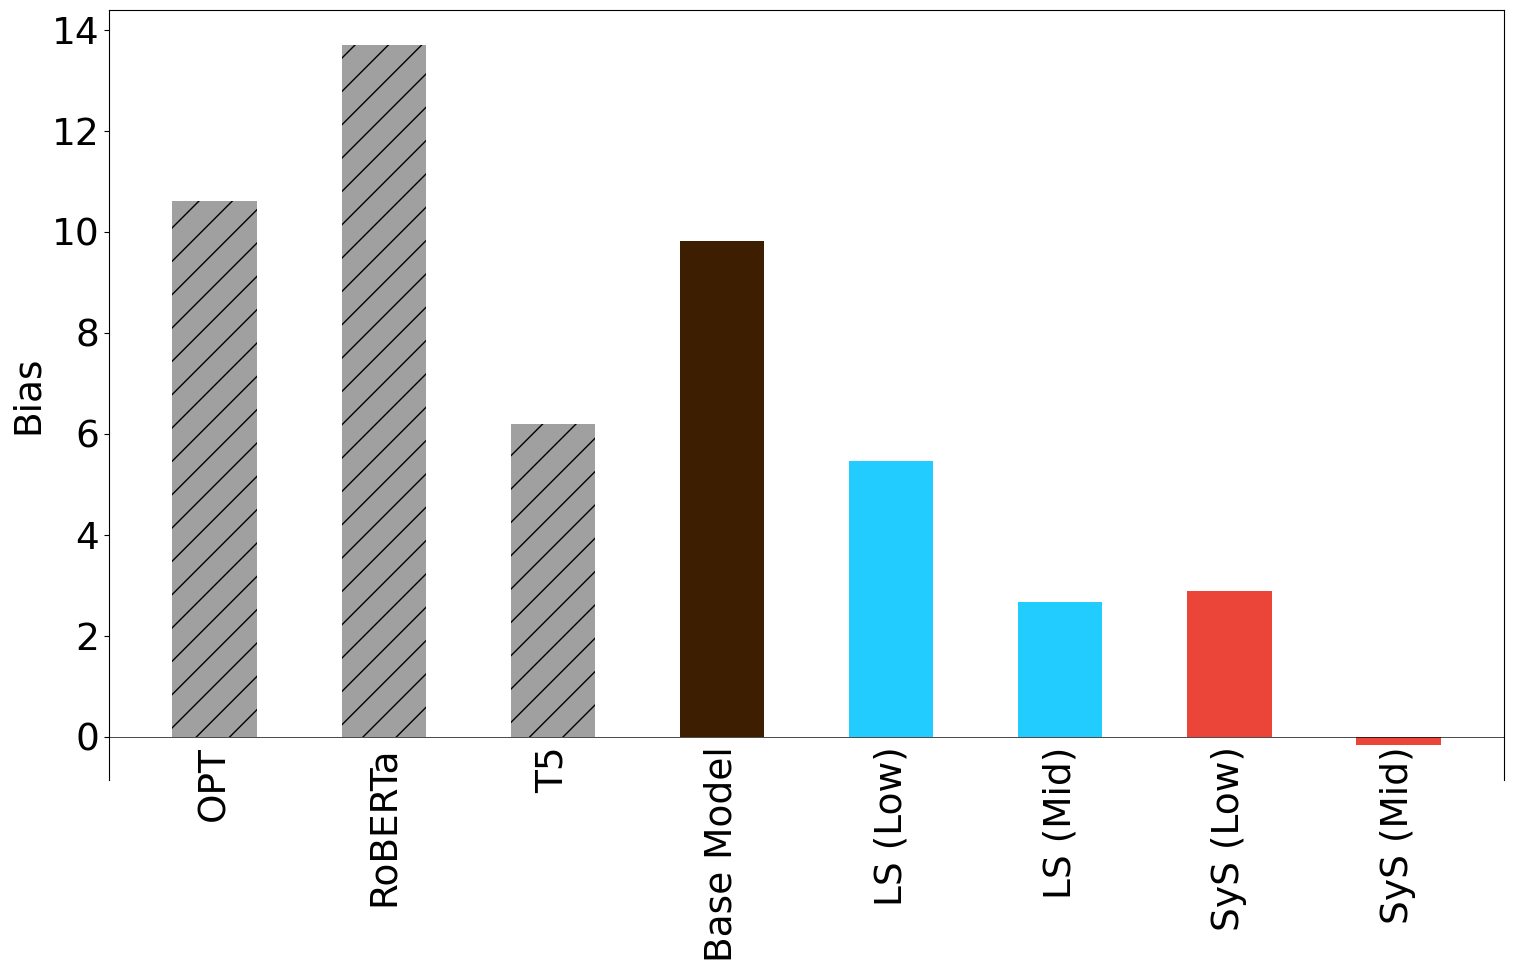
\includegraphics[width=0.5\textwidth]{chapters/syntatic-smoothing/figures/biases.png}
    \caption{Frequency bias for the three open source models, the base model, the two label smoothing (LS) baselines and the two \smoothing (\texttt{SyS}) models.}
    \label{fig:biases}
\end{wrapfigure}

I conduct analyses to inspect the learning dynamics of my method and its effect on frequency bias and anisotropy in more detail. 

\paragraph{\smoothing reduces a model's frequency bias.}
I find that all four pre-trained models exhibit strong frequency bias (see \cref{fig:biases}); they are more likely to incorrectly prefer ungrammatical sentences if they contain tokens that occur more frequently during training. This confirms the hypothesis that the evaluation of generalisation capabilities is obfuscated by frequency effects. 

By contrast, the two \smoothing variants successfully reduce the frequency bias. The frequency bias is almost completely removed in the case of the \texttt{Mid} variant, which distributes exactly half of the training signal to syntactically similar tokens. I further observe that the Label Smoothing baselines also reduce bias but to a lesser extent than the corresponding \smoothing models with the same degree of smoothing. 


\paragraph{\smoothing reduces anisotropy.}

As shown in \cref{tbl:full-results}, \newline \smoothing reduces anisotropy over both the base model and label smoothing baselines.\footnote{Note that I do not compute the anisotropy for the three open-source pre-trained models (OPT, RoBERTa, T5) because these models use different architectural configurations than the models I train (e.g., larger hidden dimensions).} Label smoothing reduces anisotropy, but not to the same extent as the \smoothing models. To better understand how anisotropy develops in a model, I compute the model's anisotropy scores at eight checkpoints during training, as shown in \cref{fig:anisotropy-learing-dynamics}. I find that a greater degree of smoothing leads to a greater reduction in anisotropy for the \smoothing variants (it is less clear if this is the case for label smoothing), supporting the hypothesis that syntactic initialization helps promote better representation learning across the model's vocabulary. I also find that the pacing method leads to lower anisotropy than the flat method, with \texttt{SyS}-P (High) achieving the lowest anisotropy throughout.

\begin{figure}[ht!]
    \centering
    \begin{subfigure}[b]{0.49\textwidth}
        \centering
        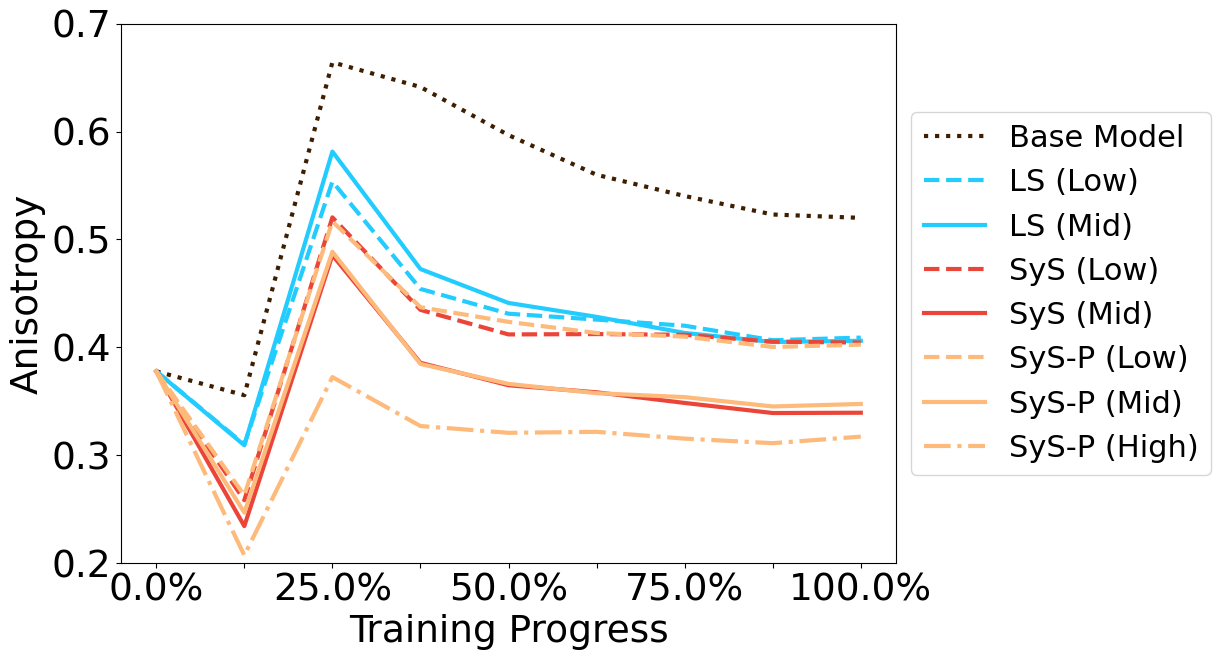
\includegraphics[width=\textwidth]{chapters/syntatic-smoothing/figures/anisotropy-learning-dynamics.png}
        \label{fig:anisotropy-learing-dynamics}
    \end{subfigure}
    \hfill
    \begin{subfigure}[b]{0.49\textwidth}
        \centering
        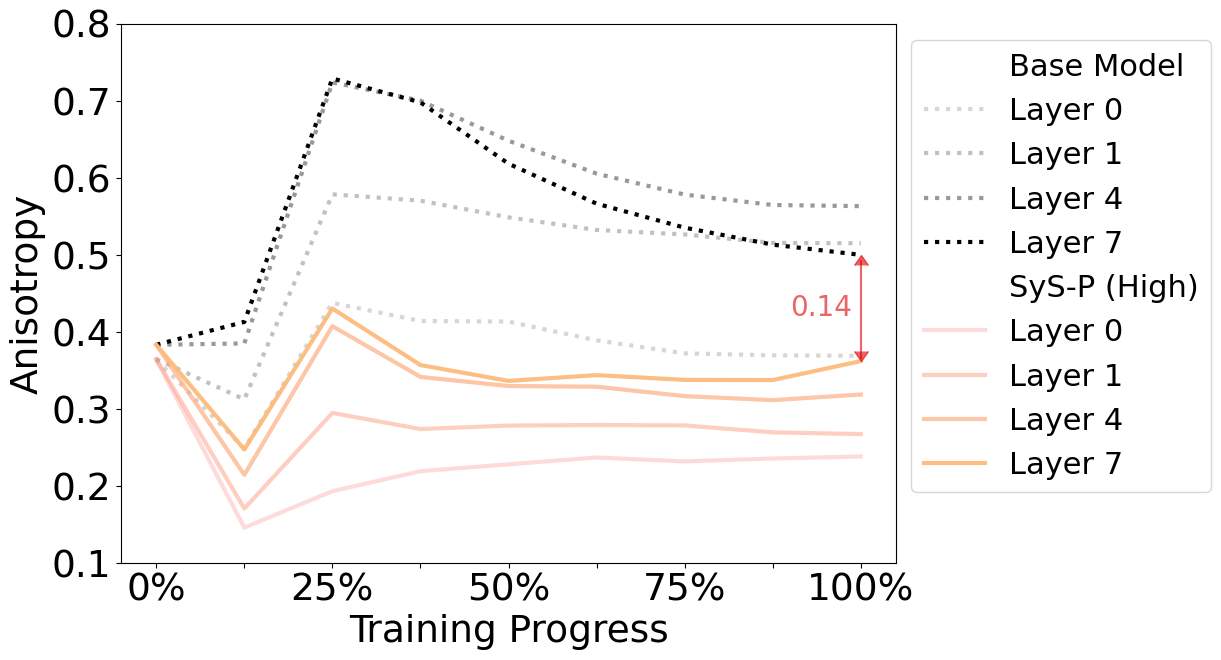
\includegraphics[width=\textwidth]{chapters/syntatic-smoothing/figures/anisotropy-layers.png}
        \label{fig:anisotropy-layers}
    \end{subfigure}
    \caption{Anisotropy learning dynamics. \textbf{Left:} Comparison of the baseline RoBERTa model, two label smoothing (LS) baselines, and the \smoothing (\texttt{SyS}) models, with values in parentheses indicating the degree of smoothing. \textbf{Right:} Anisotropy learning dynamics across selected layers for the baseline and paced \texttt{SyS} model with high smoothing, highlighting the final layer difference at the end of training.}
    \label{fig:anisotropy-combined}
\end{figure}


Over the course of training, I observe a consistent double-dip trend: an initial dip followed by a sudden rise, followed by a second slow decrease in anisotropy. The \smoothing models do not see as large a sudden rise, maintaining a lower anisotropy throughout. To examine the learning dynamics in more detail, I also plot the evolution of the anisotropy across several layers of the baseline model and the \texttt{SyS}-P (High) variant, given in \cref{fig:anisotropy-combined}. Two observations stand out. The anisotropy of all layers in the \smoothing model is lower than in the corresponding layers in the baseline model across the entire learning process. In both the baseline model and the \smoothing model, earlier layers have lower anisotropy; this finding agrees with the same observation made by \citet{ethayarajh2019contextual}. Notably, in the final layer the anisotropy of the \smoothing model remains consistently low and does not increase significantly during training, in contrast to the drastic fluctuation observed in the baseline model. This is particularly interesting as the final layer is commonly used for finetuning in downstream tasks and is empirically found to encode more high-level semantic information than the earlier layers \citep{clark2019does}. 

\paragraph{Frequency bias and anisotropy are correlated.}

For each model, I compute the model's frequency bias and anisotropy at multiple training stages. I plot the learning dynamics of anisotropy and frequency bias in \cref{fig:bias-anisotropy-correlation}, only including the points after 50\% of training has been completed to avoid the noisy first dip observed in the anisotropy dynamics above. I find a positive Pearson correlation of 0.73 and a polynomial goodness-of-fit $R^2$ score of 0.63 between these two metrics.

It is also evident that the pacing approach re-introduces frequency bias towards the end of training, as the degree of smoothing is linearly reduced to zero. It is noteworthy that the final anisotropy and bias are lower than the baseline model, and completing training without any smoothing may be beneficial for downstream tasks, as explored in the next section.

\paragraph{Frequency Bias Disproportionately Affects Content Words}
\label{section:word-class-versus-word-frequency}


To better understand the linguistic categories most impacted by frequency bias, I analyse the relationship between token frequency and syntactic class. Specifically, I compare the POS tag distributions of the top 100 most frequent tokens and the bottom 100 least frequent tokens in the training data. 

\begin{wrapfigure}{r}{0.5\textwidth}
    \centering
    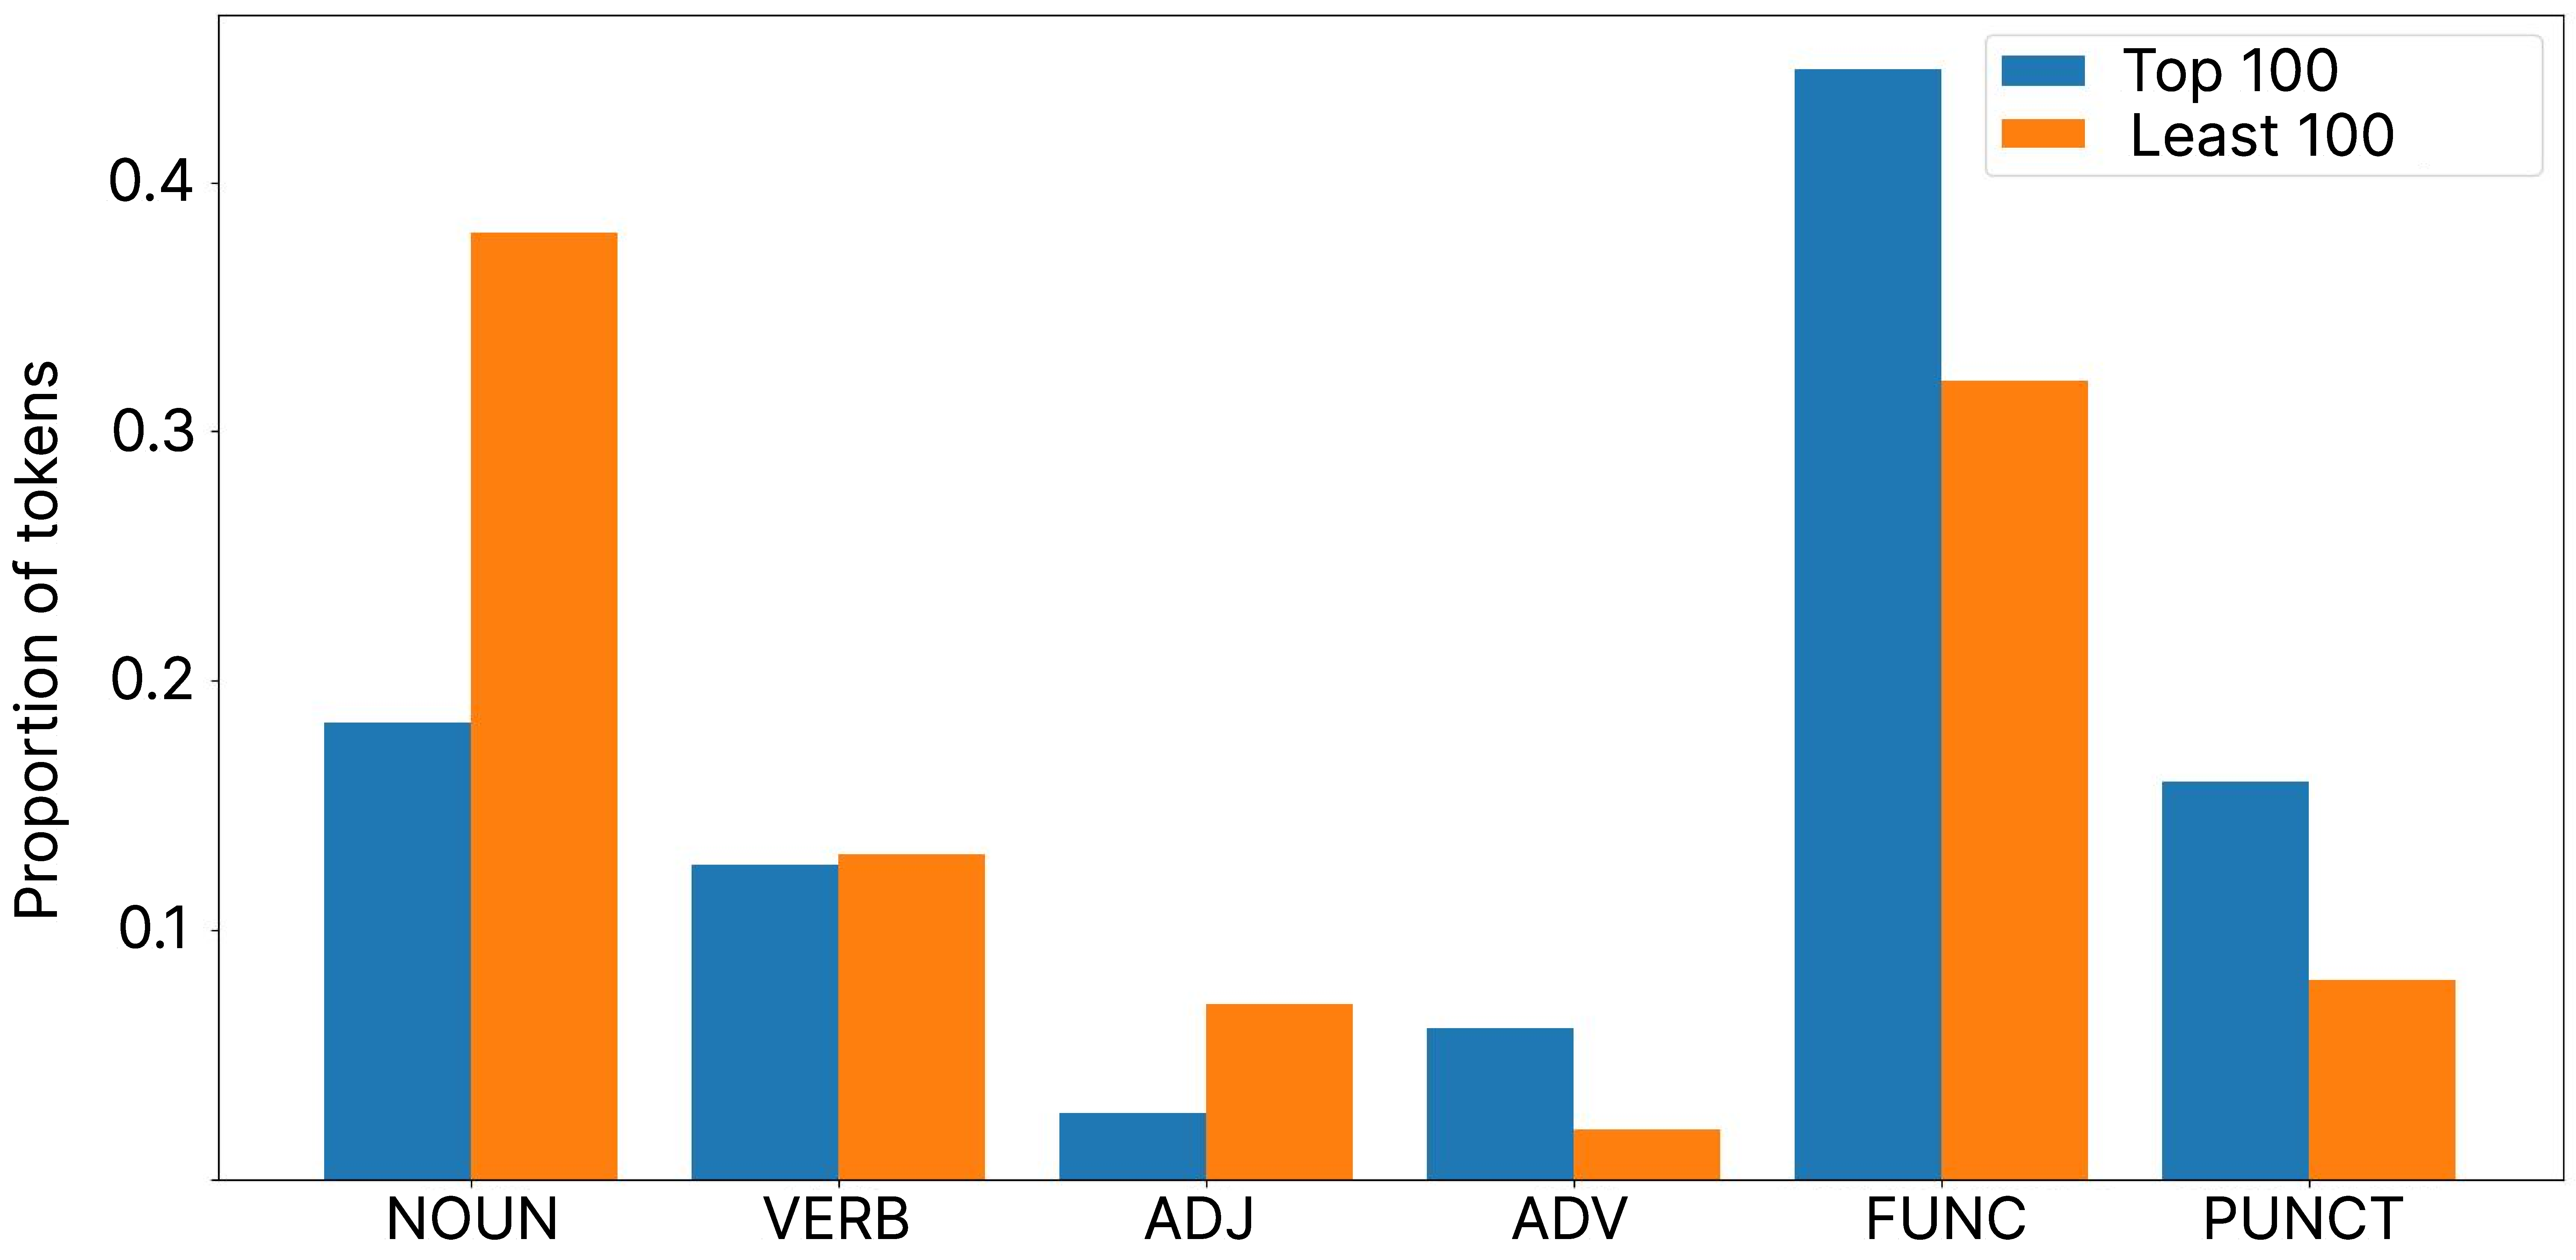
\includegraphics[width=0.49\textwidth]{chapters/syntatic-smoothing/figures/top_versus_bottom_pos_dist.pdf}
    \caption{Distribution across POS tags of the top \& bottom 100 most frequent tokens.}
    \label{fig:top-100-pos-dist}
\end{wrapfigure}

I find that content words, especially nouns, are over-represented in the low-frequency tail of the distribution, while function words dominate the high-frequency tokens. \cref{fig:top-100-pos-dist} illustrates this disparity. This suggests that frequency bias in language models may disproportionately hinder the learning of specialised vocabulary, particularly rare nouns and content-bearing expressions. It also reinforces the importance of a smoothing strategy that supports lexical generalisation by leveraging syntactic structure.

\begin{figure}[ht!]
    \centering
    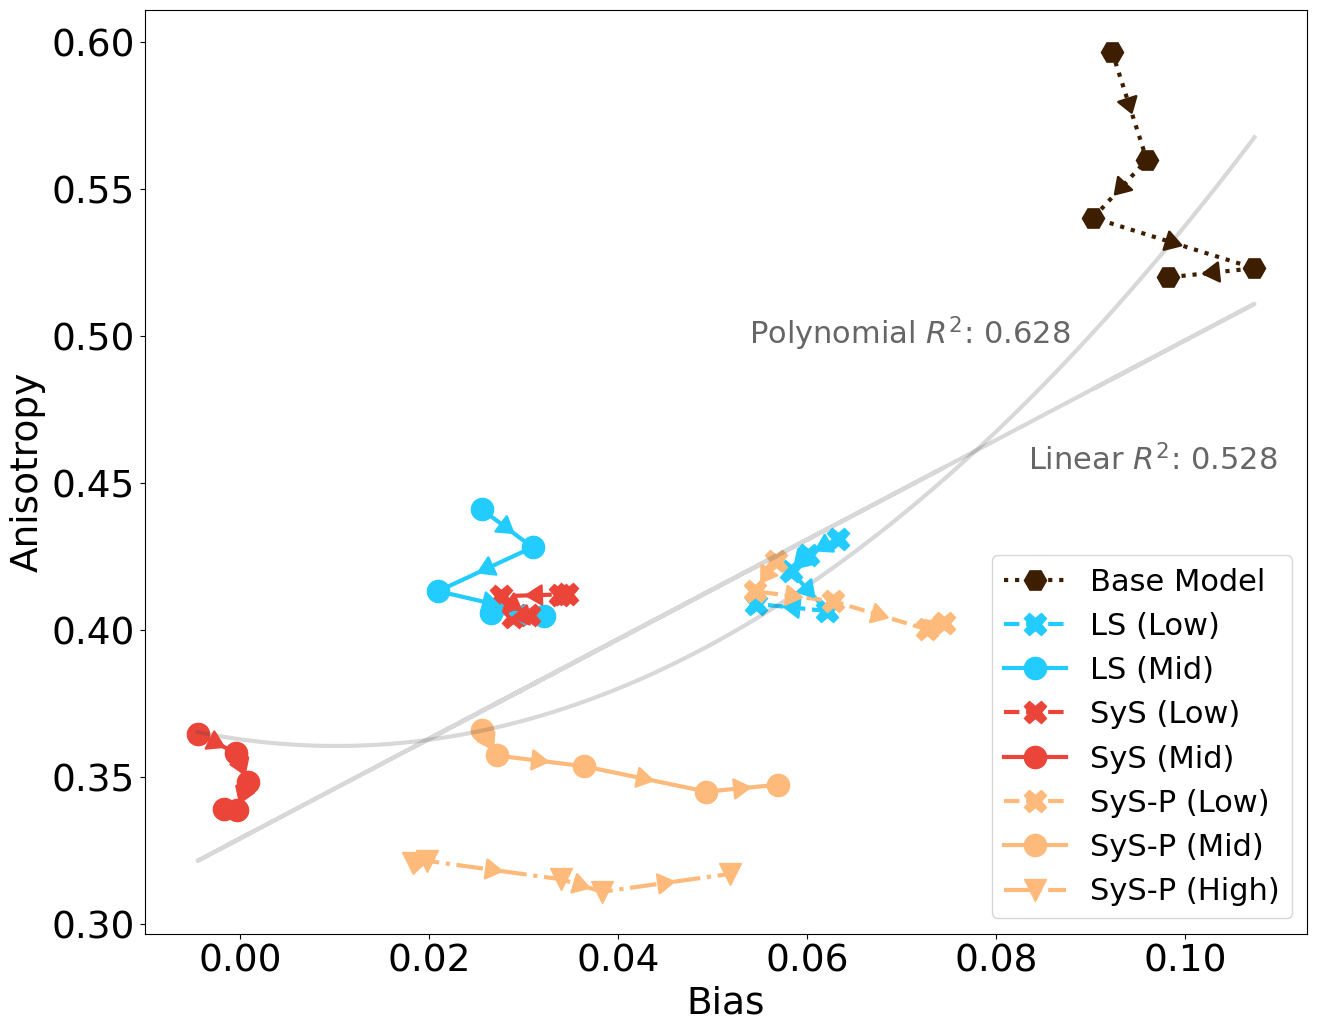
\includegraphics[width=0.75\linewidth]{chapters/syntatic-smoothing/figures/bias-vs-anisotropy.png}
    \caption{Pairs of anisotropy, and frequency bias for the baseline RoBERTa model, the two label smoothing baselines and the \smoothing models. The arrows indicate increasing training progress (starting after 50\% of training has completed).}
    \label{fig:bias-anisotropy-correlation}
\end{figure}

\subsection{Effects of Smoothing on Downstream Tasks}
While the method primarily aims to enhance the representation of infrequent tokens, I sought to investigate the potential for improvement in standard evaluation measures, given the limited number of affected test instances. Nonetheless, I observe that all the \smoothing models, as well as the label smoothing models, achieve better BLIMP scores than the baseline model (see \cref{tbl:full-results}). These results suggest that methods that smooth label distributions, whether through a syntactic prior or a simpler uniform smoothing approach, enhance the representation of all tokens, including the more frequent ones.

I had concerns that softening the frequency bias with the smoothing methododology might lead to degraded performance in downstream tasks for which frequency can be a strong proxy. As a control condition, I finetune the model on two sentence-level tasks (COLA, SST-2) and two language inference tasks (MNLI and QNLI), both of which are part of the GLUE \citep{wang2018glue} benchmark. I find that none of the \smoothing objectives result in substantial performance degradation on these NLU tasks (see the last four columns of Table~\cref{tbl:full-results}), and in fact note that for some tasks, such as SST-2, the \smoothing models yield uniform increases in performance. While not comparable apples-to-apples, I report NLU performance for the open-source baselines in \cref{tbl:full-results} as a point of reference. 

\subsection{Alternative Measures of Syntactic Similarity}

In \cref{sec:sim} I define the syntactic similarity score that is used by the \smoothing approach as the cosine similarity between POS distributions. To examine how this specific choice of similarity metric impacts my approach, I replace the cosine-based definition with a Jensen Shannon-based definition:
$$ \frac{1}{2}\big[ \text{KL}(M_i, M_j ) + \text{KL}(M_j, M_i)\big],$$
where KL$(M_i, M_j)$ is the Kullback-Leibler divergence between the POS distributions, $M_i$ and $M_j$, for the vocabulary items $V_i$ and $V_j$.

\begin{table}[ht!]
\centering
\small
\begin{tabular}{l||cc|ccccc}
\toprule
\textbf{Model}  &  \textbf{Bias}  & \textbf{Anisotropy} & \textbf{BLiMP} \\
\midrule
Base Model & 9.8 & 51.3 & 71.4  \\
\midrule
\texttt{SyS} (Mid) \hspace{0.42cm} [JS]  & 3.6 & 34.7 & 71.3 \\
\texttt{SyS} (Low) \hspace{0.38cm} [JS]  & 4.1 & 34.6 & 73.3  \\
\texttt{SyS}-P (High) \hspace{0.05cm} [JS] & 6.6 & 36.7  & 72.5  \\ 
\texttt{SyS}-P (Mid) \hspace{0.15cm} [JS] & 8.4 & 39.1 &  73.0 \\ 
\texttt{SyS}-P (Low) \hspace{0.12cm} [JS] & 5.0 &  34.5 & 72.9 \\ 
\bottomrule
\end{tabular}
\caption{\label{tbl:jsd-similarity-metric-results}
Results for bias~($\downarrow$), anisotropy~($\downarrow$), and BLiMP~($\uparrow$) score for \smoothing (\texttt{SyS}) models that use a Jensen Shannon-based [JS] definition of the similarity metric.}
\end{table}

Summarised in \cref{tbl:jsd-similarity-metric-results}, I note that the effect of using a Jensen Shannon-based definition of the similarity metric yields a similar (albeit slightly smaller) decrease in frequency bias and anisotropy, as compared to the standard cosine-based definition of the similarity metric.   

\section{Conclusion}
\label{sec:conclusion}

This chapter has addressed a core limitation of current language models: their difficulty in generalizing to rare or novel words due to an overreliance on frequency statistics. While human learners can infer grammatical roles and meanings from structural context, a process often referred to as syntactic bootstrapping, most language models lack this inductive bias. As a result, they tend to prioritise high-frequency tokens, leading to frequency bias and degraded representations of infrequent words.

I proposed \smoothing, a cognitively motivated training method that distributes the learning signal for each token across other syntactically similar tokens. Using part-of-speech distributions as a simple approximation for syntactic similarity, this approach allows low-frequency tokens to benefit from the learning dynamics of more frequently observed counterparts. In doing so, it operationalises the human strategy of learning by structural association.

To evaluate this method, I introduced a new diagnostic for frequency bias, measuring the degree to which a model incorrectly prefers ungrammatical but frequent alternatives. I found that \smoothing significantly reduces this bias and also decreases anisotropy in the representational space. These gains were achieved without sacrificing downstream task performance, suggesting that structural cues can support lexical generalisation even in small-scale or low-resource training settings.

By connecting insights from cognitive science with concrete modifications to training, this chapter moves beyond architectural changes and explores how the learning process itself can be made more human-like. If curriculum learning structures what is learned and when, \smoothing focuses on how internal representations evolve to support abstraction and generalisation.

In the next few chapters, I take a closer look at this learning process. How do language models internalize linguistic structure over time? What patterns of learning emerge during training, and how do they compare to those observed in human learners? Building on the methods introduced here, I now turn to analysing the dynamics of learning within neural language models.


% PART 2 

\part{An Analytical Lens on Learning Dynamics}
\chapter{Analyzing Language Models: Foundations, Methods, and Tools}
\label{sec:analysis-background}

Understanding how language models learn, represent, and generalize linguistic knowledge requires a diverse set of analytical approaches. This chapter surveys foundational work in three interrelated areas: (1) attention-based and representational interpretability, (2) mechanistic interpretability that aims to reverse-engineer internal computations, and (3) learning dynamics research that tracks how capabilities emerge over time during training. 

Our emphasis is especially on methodologies that provide insight into the internal mechanisms of transformer-based models, with a focus on tools that are most relevant to understanding small models and their developmental trajectories. Throughout the chapter, we highlight key techniques for probing attention heads, decomposing learned circuits, tracking convergence and capacity usage, and analyzing models across training checkpoints and scales.

We also introduce the growing ecosystem of open-source model suites and analysis frameworks that enable this work—resources that make it possible to observe, quantify, and intervene in learning dynamics directly. These tools will form the empirical and methodological foundation for the contributions in the next chapters, where we analyze how small models diverge from larger ones and propose interventions to improve their learning behavior.
\section{Analysis of Attention}

The transformer architecture brought the attention mechanism to the forefront of representation learning. Early efforts to interpret these models focused on analyzing attention patterns to uncover what linguistic information models capture and how it is distributed across their components.

\subsection{Multi-Head Attention Analysis}

Early efforts to understand transformer models focused heavily on analyzing attention patterns—both to probe internal representations and to assess model efficiency.

A foundational study by \citet{voita2019analyzing} showed that attention heads in transformer models often specialize in distinct linguistic roles, such as syntactic dependencies, coreference, and discourse relations. This head-level specialization pointed to an emergent modularity, where different heads implicitly divide up the task of language processing.

Crucially, they also demonstrated that many heads could be pruned with minimal impact on downstream performance, suggesting that only a subset are essential. This insight laid the groundwork for head pruning as a principled form of model compression.

\citet{michel2019sixteen} expanded on these findings by empirically measuring redundancy among attention heads. They showed that despite being designed for parallel attention, many heads capture overlapping information, reinforcing the sparsity hypothesis and motivating leaner transformer designs.

Building on these analytical approaches, \citet{clark2019does} developed visualization methods for interpreting attention in BERT. Their study found that BERT’s attention heads capture both syntactic and semantic relationships—for instance, tracking subject-verb agreement or coreference chains. This work helped establish attention weights as interpretable proxies for internal reasoning, turning attention visualization into a widely used diagnostic tool in transformer research.

\subsection{Sparse Probing}

While attention-based methods offer a window into model behavior, other approaches have investigated how linguistic structure is embedded in hidden representations. \citet{hewitt2019structural} introduced a structural probe to test whether contextual embeddings encode syntactic information such as dependency trees. Their results showed that BERT's middle layers encode rich syntactic structure in a geometrically meaningful way, revealing that grammar is implicitly embedded in the model's representational space.

More recently, \citet{gurnee2023finding} proposed sparse probing—a technique that constrains linear probes to use only a small number of neurons, enforced via $L_0$ regularization. Their results suggest that linguistic features, while broadly distributed, can be reliably recovered from sparse subsets of neurons. This highlights the potential for localized interpretability, particularly relevant for small models where transparency is more attainable.

\section{Mechanistic Interpretability}

While sparse probing offers a high-level view of which neurons encode linguistic features, mechanistic interpretability aims to reverse-engineer how those features are computed—tracing internal mechanisms such as circuits, neurons, and layer interactions that give rise to model behavior.

\subsection{Foundational Ideas and Circuits}

\begin{figure}[ht!]
    \centering
    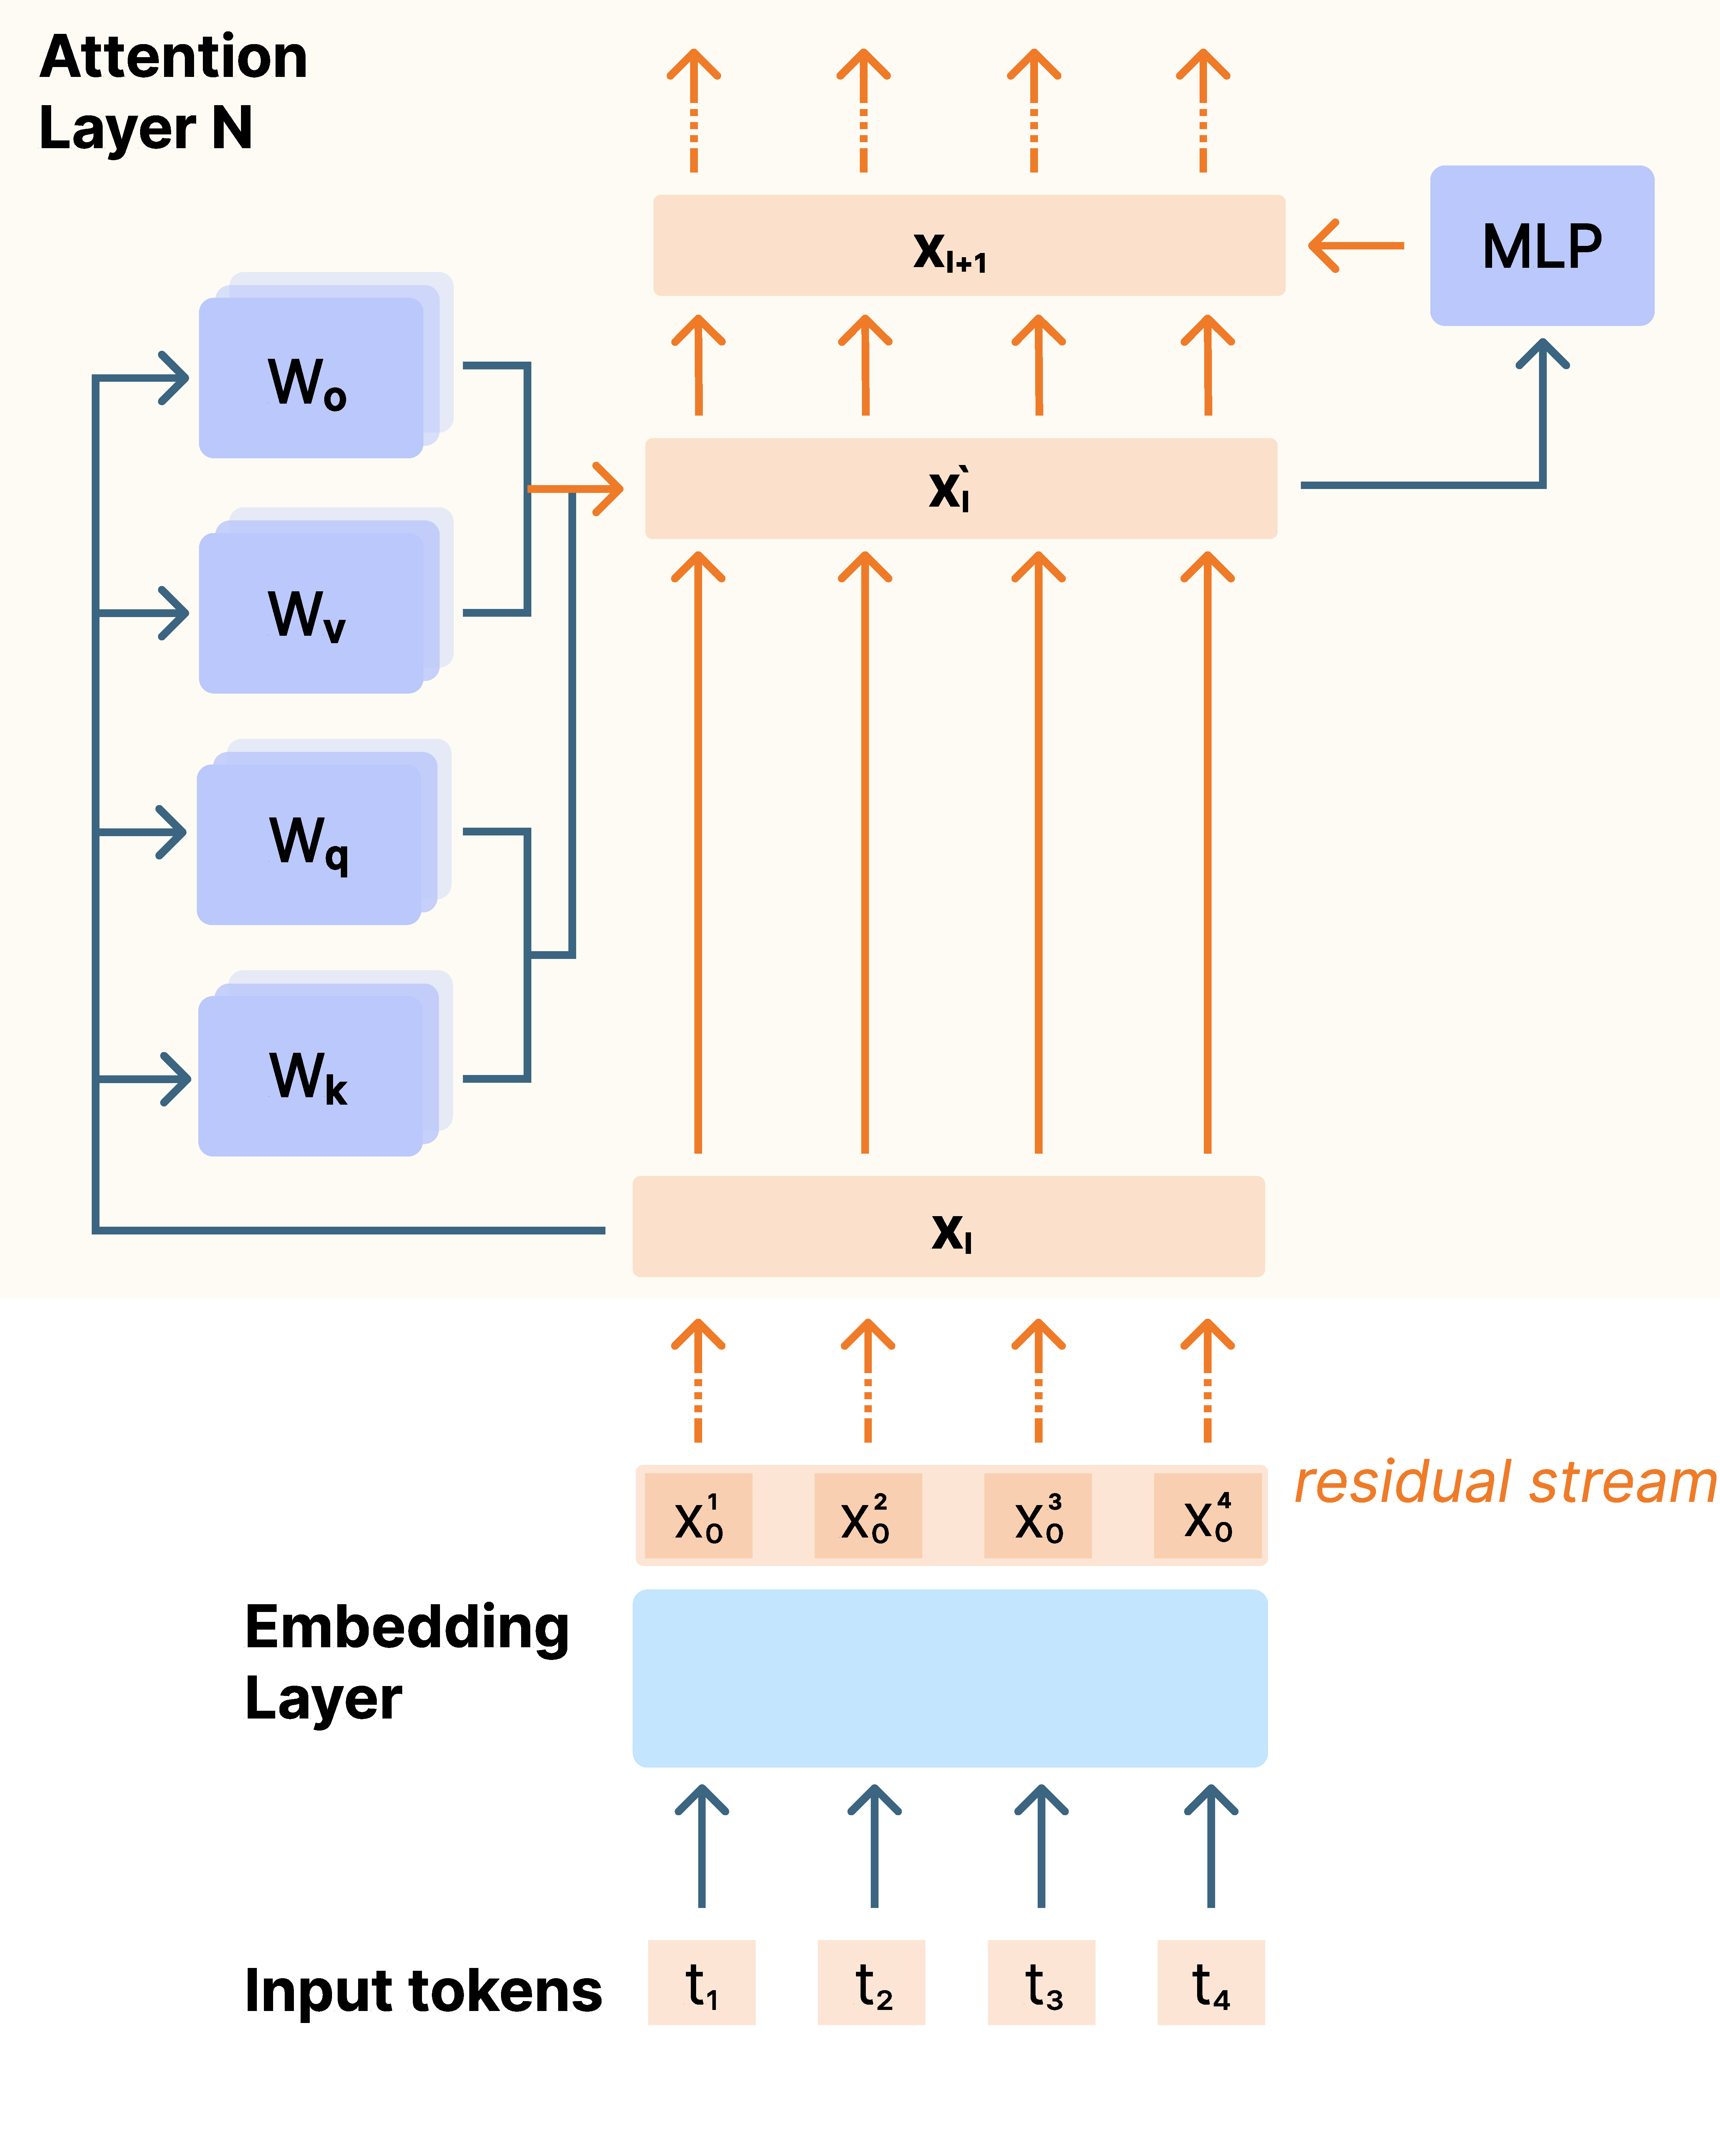
\includegraphics[width=0.6\textwidth]{chapters/analysis_background/figures/residual_stream_visualization.pdf}
    \caption{Visualization of the residual stream in a transformer model, showing how information flows through the network via skip connections and is progressively refined through attention and feed-forward layers.}
    \label{fig:residual-stream}
\end{figure}


The theoretical foundations of this field were laid by \citet{olah2014manifolds}, who framed neural networks as systems that deform data manifolds while preserving topological structure. This perspective provides a conceptual basis for interpreting how deep models process and transform information layer by layer.

Building on this, \citet{elhage2021mathematical} introduced a formal framework for decomposing transformers into interpretable circuits. Using tools like “virtual weights,” they showed how specific attention heads can implement distinct algorithms—such as copying or positional induction—forming structured computational graphs within the model. These operations are executed within the shared residual stream, a central component of transformer architecture that carries forward and combines layer outputs across the model.

The residual stream is a mathematical formalization through which to study how transformer models process inputs \citep{elhage2021mathematical}. Under this framework, each of the $L$ layers of a transformer model processes a series of input tokens $\sequence = \langle \token_1, \smalldots, \token_\seqlen\rangle$ consecutively and communicates the result of its computation for each token to subsequent layers via a residual stream of dimension $\residualdim$. 

The reading, processing, and writing of the residual stream occur independently in each $\attention$ head via combinations of the query, key, value, and output matrices, $W_Q$, $W_K$, $W_V$, $W_O$. The \textbf{query-key circuit}, $W_Q^{\top}W_K$, of the $\attention$ mechanism controls how the residual stream should be recomposed, and the \textbf{output circuit}, $W_OW_V$, writes to the residual stream an update that is mediated by the query-key circuit. The write operation of each $\attention$ head is of low rank relative to $\residualdim$. After each $\attention$ head has written to the residual stream, a bottleneck $\mlp$ projection performs a full-rank transformation on the residual stream. Due to their pivotal role in updating the state of the residual stream, our work analyzes the learning dynamics of the two operations that write to the residual stream: the output circuit of each head of the $\attention$ layer---that we refer to as $\attention$---and the $\mlp$ projection layer---that we denote $\mlp$ for conciseness.

As illustrated in \cref{fig:residual-stream}, the residual stream serves as the backbone of computation, enabling attention and feed-forward layers to progressively refine and update internal representations at each layer.

A key example of this modular behavior is the “induction head” described by \citet{olsson2022inductionheads}, which performs in-context learning by detecting repeating token patterns. Their work demonstrated that induction heads are universal across transformer models and emerge consistently during training, highlighting how meaningful algorithmic structure can arise within the residual stream.

\subsection{Representation, Superposition, and Memory}

Neural networks often represent multiple features in overlapping activation dimensions—a phenomenon known as superposition. \citet{elhage2022toy} formalized this idea and showed how it creates both efficient storage and representational interference. They proposed sparse coding as a way to reduce overlap and improve interpretability.

Complementary work by \citet{geva2021memory} reframed feed-forward layers as key-value memory stores, where neurons act as retrievable content-addressable memories. This perspective highlights how information retrieval occurs outside the attention mechanism, reshaping our understanding of transformer architecture.

\citet{dai2022knowledge} further explored how factual information is stored in “knowledge neurons”—units that encode specific facts in a distributed but partially localizable way. These findings reinforce the idea that interpretability is possible even in large, dense models, particularly through targeted neuron analysis.

\subsection{Toward Full Decomposition}

Recent efforts have focused on decomposing model activations into monosemantic features—components that represent a single, interpretable concept. \citet{bircken2023monosemanticity} applied sparse autoencoders to learn such features from model activations, revealing interpretable directions in activation space. This method shows promise for mitigating superposition and improving transparency.

\citet{anthropic2023components} outlined a broader research vision for full model interpretability, where each parameter's role is understood. Their approach leverages dictionary learning and modular decomposition to identify circuits, features, and neurons aligned with human-understandable behaviors.

\subsection{Tools for Intermediate Layers and Model Analysis}

To support these interpretability efforts, a range of tools and frameworks have emerged.

\citet{belrose2023eliciting} developed the Tuned Lens, an extension of the logit lens, which improves interpretability of intermediate layers by learning linear probes that better approximate the model's output predictions at earlier stages. This allows for clearer analysis of how information evolves through the network.

\citet{nanda2022transformerlens} introduced TransformerLens, a library for inspecting transformer internals—including attention heads, MLP layers, and residual streams. It is widely used for circuit-level analysis, enabling researchers to trace forward and backward signals through static, trained models.

Several tools also support causal and structural interventions. \citet{meng2022locating} proposed ROME, a technique for directly editing factual knowledge in a trained transformer by locating and modifying causal neurons. Similarly, \citet{conmy2023towards} developed ACDC, which uses sparse matrix factorization to automatically extract circuits from models, enabling inference-time interpretability without retraining.

For broader attribution analysis, \citet{kokhlikyan2020captum} developed Captum, a general-purpose library for feature attribution in PyTorch. While not transformer-specific, it includes a suite of interpretability tools—such as Integrated Gradients and DeepLIFT—that are useful for probing feature importance across different model architectures.



\section{Developmental Interpretability}
While mechanistic interpretability reveals the internal structure of trained models, developmental interpretability shifts focus to how those structures emerge during training. By analyzing checkpoints over time, this approach captures the trajectory of learning—offering insight into when and how linguistic capabilities arise.

\citet{hoogland2023towards} introduced this paradigm by identifying phase transitions in learning, supported by the Local Learning Coefficient as a measure of representational complexity. Building on this, \citet{hoogland2025losslandscape} connected stagewise learning to loss landscape geometry, revealing that shifts in capability often align with flat or degenerate regions in the optimization surface.

To support empirical analysis, \citet{devinterpcode} developed DevInterp, a toolkit for tracking model development over time. Together, these contributions establish developmental interpretability as a powerful complement to static and circuit-based approaches—highlighting not just what models learn, but when and how they acquire it.

This developmental perspective naturally leads into a broader field of inquiry: learning dynamics—the study of how language models acquire, retain, and organize knowledge over time.

\section{Developmental Interpretability}
While mechanistic interpretability reveals the internal structure of trained models, developmental interpretability shifts focus to how those structures emerge during training. By analyzing checkpoints over time, this approach captures the trajectory of learning—offering insight into when and how linguistic capabilities arise.

\citet{hoogland2023towards} introduced this paradigm by identifying phase transitions in learning, supported by the Local Learning Coefficient as a measure of representational complexity. Building on this, \citet{hoogland2025losslandscape} connected stagewise learning to loss landscape geometry, revealing that shifts in capability often align with flat or degenerate regions in the optimization surface.

To support empirical analysis, \citet{devinterpcode} developed DevInterp, a toolkit for tracking model development over time. Together, these contributions establish developmental interpretability as a powerful complement to static and circuit-based approaches—highlighting not just what models learn, but when and how they acquire it.

This developmental perspective naturally leads into a broader field of inquiry: learning dynamics—the study of how language models acquire, retain, and organize knowledge over time. But developmental interpretability is just one part of a broader movement toward training-time analysis. To fully understand how language models acquire and organize their capabilities, we need a more expansive view—one that considers not just phase transitions, but also how examples are memorized or forgotten, how representations converge, how capacity is allocated, and how internal structures evolve in rank and geometry.

\section{Learning Dynamics Research}

Understanding how language models learn—beyond just what they ultimately represent—is central to both interpretability and model development. Learning dynamics research investigates the evolving internal behavior of models throughout training, revealing how linguistic capabilities emerge, stabilize, or fail to develop.

This work spans a diverse set of analytical perspectives, each offering insights into different facets of training-time behavior.

\subsection{Memorization and Data Influence Analysis}

A central goal in learning dynamics is to understand how specific examples affect learning over time—whether they are memorized, generalized, or forgotten.

Influence functions, introduced by \citet{koh2017understanding}, trace the effect of individual training examples on model predictions by approximating parameter updates through gradients and inverse Hessians. \citet{grosse2023influence} extended this method to large language models, enabling counterfactual analysis: how would the model behave if a given sequence were added to the training set?

Complementary to this, prediction trajectory methods analyze how model outputs evolve across training steps. \citet{toneva2019empirical} introduced the concept of forgetting events—when a model switches from correct to incorrect on a training example—offering a lens on stability and difficulty. \citet{swayamdipta2020dataset} expanded this idea with dataset cartography, classifying examples by prediction confidence and variability to map learning trajectories across NLP datasets.
\citet{feldman2020does} examined the tradeoff between memorization and generalization, especially in smaller models where memorization may be necessary for strong performance. \citet{biderman2023emergent} investigated verbatim memorization in the Pythia model suite, finding that early checkpoints can effectively forecast what large models will eventually memorize—though smaller models cannot.

Together, these approaches reveal that memorization is shaped by training dynamics, model scale, and the specific properties of the data.

\subsection{Convergence and Representation Similarity}

While memorization-focused analyses emphasize how individual examples influence a model's behavior, convergence analysis shifts attention to the evolution and stabilization of internal representations during training. This research area seeks to understand when and how model layers begin to encode stable linguistic abstractions, how representational structures develop over time, and the extent to which different models (trained on the same or different data) develop similar internal solutions.

\subsubsection{Measures of Representational Similarity}

A foundational family of methods in this space builds on \textit{Canonical Correlation Analysis (CCA)}, which compares the similarity between two multivariate representations. In neural networks, this allows researchers to quantify the alignment between layer activations at different checkpoints, across different models, or within different layers of the same model. \citet{raghu2017svcca} introduced \textit{Singular Vector CCA (SVCCA)}, which first reduces the dimensionality of representations via singular value decomposition before applying CCA to the resulting principal components. This makes the method more robust to noise and scale differences in deep representations. However, SVCCA has limitations in terms of sensitivity and interpretability.

To address these limitations, \citet{morcos2018pwcca} proposed \textit{Projection-Weighted CCA (PWCCA)}, which weights the contribution of each component according to how much it aligns with the original data. This technique down-weights noisy or low-signal components, yielding a more faithful measure of similarity. Despite these refinements, CCA-based methods still struggle in settings where the representation dimensionality exceeds the number of datapoints---a common scenario in large-scale models with deep layers and high-dimensional embeddings.

To overcome this, \citet{kornblith2019cka} introduced \textit{Centered Kernel Alignment (CKA)}, a method based on kernel similarity that offers greater robustness across dimensional regimes. In its linear form, CKA computes the similarity between two activation matrices \( X, Y \in \mathbb{R}^{n \times d} \) as:

\[
\mathrm{CKA}(X, Y) = \frac{\| Y^\top X \|_F^2}{\| X^\top X \|_F \cdot \| Y^\top Y \|_F}
\]

where \( \|\cdot\|_F \) denotes the Frobenius norm. This measure is invariant to orthogonal transformations and isotropic scaling of the representations, making it well-suited for comparing different models or different training stages. CKA has since become a standard tool for tracking representational convergence in both vision and language models.

While CKA and CCA focus on representational similarity in a static sense, another approach---\textit{model stitching}---investigates whether different models are \textit{functionally} equivalent at certain layers. Originally proposed by \citet{lenc2015understanding} for convolutional networks, this method was later formalized by \citet{bansal2021stitch} as a technique for connecting the lower layers of one model to the upper layers of another, using a small trainable adapter in between. If the stitched model performs well, it suggests that the internal representations of the two models are sufficiently aligned to be interoperable. Stitching provides a more dynamic view of convergence, capturing not just alignment in activation space but also compatibility in downstream processing.

\subsubsection{Applications to Language Models}

These methods have been extensively applied to \textit{language models} to understand the progression and stability of learned representations. For instance, \citet{saphra2019understanding} used SVCCA to track the alignment of ELMo's hidden states with syntactic annotations, finding that parts-of-speech (POS) information is learned early in training and primarily encoded in lower layers. Similarly, \citet{singh2019bert} applied CCA to multilingual BERT and discovered that representations in the deeper layers diverge across languages, forming hierarchical clusters that reflect known linguistic relationships---suggesting that BERT learns distinct structural priors for different languages.

More recent work by \citet{nguyen2020wide} and \citet{phang2021finetuned} used CKA to identify \textit{block structure} within deep transformers, where layers cluster into groups that share similar representations. These structures are especially pronounced in larger models and later in training, where adjacent layers often encode similar abstractions. \citet{wu2020similarity} found that models from the same architecture family tend to exhibit stronger representational similarity, even if individual neurons vary---suggesting shared inductive biases across architectures. Finally, \citet{brown2023understanding} analyzed intra- and inter-model similarity within the Pythia model suite, using CKA to identify both convergence points and divergence in representation trajectories over time. Their findings support the idea that convergence is not uniform across training but rather unfolds in stages that reflect changes in capacity utilization, generalization, and abstraction.

In summary, convergence analysis provides a global view of how language models evolve during training---not at the level of individual examples, but at the level of their internal geometry. Techniques such as CKA, PWCCA, and model stitching offer complementary insights into how and when models develop aligned representations, how stable those representations are, and to what extent learned abstractions are transferable. These tools are especially valuable in the study of small models, where transparency and structure are more accessible and where representational convergence can serve as a guide for diagnosing inefficiencies, bottlenecks, or missed opportunities in training.

\subsection{Sparsity and Norms Analysis}

While convergence analysis provides a high-level view of how internal representations stabilize over time, another important dimension of learning dynamics concerns how models manage and allocate their \textit{capacity}—both in terms of which parameters are used and how their magnitudes evolve. Analyses of \textit{sparsity} and \textit{norms} offer fine-grained insight into how models compress information, avoid redundancy, and maintain stable training.

This line of work investigates not only how sparsity emerges during training, but also how different types of norms—such as activation norms, weight norms, and gradient scales—fluctuate and influence model behavior. Together, these metrics help reveal how language models balance expressivity with efficiency and stability.

\subsubsection{Sparsity Metrics and Analysis}

A foundational contribution to the measurement of sparsity came from \citet{hoyer2004sparsity}, who proposed a continuous sparsity score that combines the \( \ell_1 \) and \( \ell_2 \) norms of a vector. This \textit{Hoyer's sparsity} metric ranges from 0 (fully dense) to 1 (maximally sparse), making it particularly effective for tracking the emergence of sparse representations in activation maps or weight matrices during training. Its simplicity and interpretability have made it widely adopted in analyzing deep networks, including transformers.

\citet{hurley2009gini} evaluated various sparsity measures from a theoretical perspective, outlining six desirable properties such as scale and permutation invariance. They showed that both the Gini coefficient and Hoyer’s metric satisfy these criteria, validating their robustness for analyzing sparsity in neural models.

\subsubsection{Functional Sparsity in Language Models}

Beyond abstract metrics, several studies have explored \textit{functional sparsity}: how neural models naturally deactivate or underutilize certain components during training. \citet{frankle2019lottery} introduced the \textit{lottery ticket hypothesis}, showing that sparse subnetworks within overparameterized models can achieve full performance if trained in isolation. This finding sparked a wave of interest in understanding which parameters are actively contributing to learning and which are not.

Building on this, \citet{michel2019sixteen} found that many attention heads in transformers can be pruned without degrading performance—suggesting redundancy in head usage and an opportunity for model compression. \citet{voita2019analyzing} confirmed this by introducing \textit{head importance scoring}, showing that some attention heads specialize in interpretable functions while others effectively deactivate, illustrating emergent sparsity during training.

\citet{evci2020rigging} analyzed the training trajectories of sparse networks and found that early training phases are especially unstable when sparsity is enforced too aggressively. This underscores the importance of understanding when sparsity is beneficial and how it interacts with training dynamics.

More recently, \citet{jiang2023pruning} proposed sparsity-aware pruning strategies tailored to pretrained transformers, focusing on neurons that become saturated, unused, or ``dead'' over the course of training. Their work provides practical tools for diagnosing inefficiencies in model capacity usage.

\subsubsection{Norm Evolution and Training Stability}

Complementing sparsity analysis, research into \textit{norm dynamics} offers insight into the scaling and stability of model parameters and activations. \citet{mishkin2016goodinit} studied how weight and activation norms evolve during training and highlighted the role of proper initialization and normalization (e.g., LayerNorm) in maintaining stable learning. Their findings are particularly relevant in transformer architectures where residual pathways can lead to norm drift.

\citet{liu2020understanding} examined \textit{gradient and activation norm instability} in transformers, identifying early-phase training as especially vulnerable to vanishing or exploding norms—an issue especially pronounced in smaller models. These instabilities can explain training failures and motivate adjustments to learning rates, normalization, or initialization strategies.

From a theoretical angle, \citet{arora2018theoretical} connected parameter norm growth to generalization bounds, suggesting that norm-based proxies can signal overfitting or underfitting. Meanwhile, \citet{zhang2021calibration} studied \textit{logit norms} as a proxy for model confidence, showing that poorly calibrated models tend to have misaligned norm dynamics at the output layer. Their findings highlight how monitoring output norm evolution can inform assessments of prediction reliability during training.


\subsection{Rank and Geometry Analysis}

Beyond parameter count or loss metrics, understanding how many dimensions a model \textit{actually uses} to represent information reveals important dynamics of learning and capacity utilization. Rank and geometry analysis captures how representational complexity evolves during training, identifies learning phase transitions, and highlights inefficiencies in model design—particularly in small or overparameterized models.

Training often unfolds in distinct stages, each marked by shifts in representational rank. \citet{boix-adsera2023rank} showed that transformer weights increase in rank incrementally from initialization, mirroring stepwise acquisition of complexity. \citet{belrose2024neural} further observed that models progressively encode more sophisticated statistical patterns—starting from unigrams and advancing toward syntax—suggesting stagewise curriculum-like learning.

Structural limits also constrain learning. \citet{godey2024small} found that small language models hit a representational bottleneck at the output layer: the softmax saturates in rank even while loss continues to fall. This suggests underperformance may stem from expressivity ceilings, not optimization failure.

To characterize these dynamics, researchers have proposed several ways to estimate how many dimensions a model \textit{functionally} uses. \citet{garg2025utilizedrank} introduced \textit{utilized rank}, which estimates the number of active dimensions in a layer's weight matrix by projecting it onto input/output subspaces derived from real data. Their analysis showed that many large models use only a small fraction of their nominal capacity—e.g., ViT-L/16 utilizes just $\sim$20\% of its available rank.

Another approach is \textit{effective rank}, a continuous measure of dimensionality based on the entropy of a matrix's singular values \citep{roy2007effectiverank}. Given singular values $\sigma_1, \dots, \sigma_r$, normalized as $p_i = \frac{\sigma_i}{\sum_j \sigma_j}$, effective rank is defined as:

\[
\mathrm{erank}(A) = \exp\left(-\sum_{i=1}^r p_i \log p_i\right)
\]

This metric ranges from 1 (collapsed representation) to $r$ (full rank), offering a smooth, interpretable way to track representational complexity. We adopt this measure in later chapters to analyze the learning dynamics of small language models.

Multiple studies have observed discrete jumps in effective rank, closely aligned with drops in training loss—a phenomenon termed the \textit{rank staircase} by \citet{yang2024rankstaircase}. These transitions mark key inflection points in the learning process, supporting the idea that training progresses in qualitatively distinct stages.

More broadly, rank-based analyses suggest that low-rank structure is an emergent property of training itself. \citet{pellegrino2023lowrank} found that both biological and artificial networks tend to evolve along low-dimensional subspaces. \citet{feng2022rank} and \citet{minyoung2022lowrank} provide theoretical support, showing that neural networks exhibit a bias toward rank-deficient representations and structurally simple solutions.

In sum, rank and geometry analysis deepens our understanding of how language models acquire, compress, and allocate representational capacity. These tools shed light on inefficiencies in training and architecture and serve as valuable diagnostics for learning progression. Later chapters build on this foundation, using effective rank to study capacity bottlenecks and phase transitions in small model training.

\section{Frameworks and Tools for Learning Dynamics Research}

Understanding how language models learn requires visibility into the training process itself. This is especially critical when comparing how models of different sizes acquire capabilities, converge to solutions, or fail to do so. Smaller models often underperform not because of optimization failure, but due to structural limitations and divergence in learning trajectories. To study these differences, researchers increasingly rely on model suites that expose internal states over time and across scales.

This section surveys a set of frameworks that make such investigations possible. These resources are essential for answering \textbf{Research Question 2:} \textit{How can we more quantitatively understand how small models learn and what makes them different from large models?} By enabling cross-scale comparisons, these tools help reveal when and why smaller models diverge, and support targeted hypotheses for making their learning dynamics smoother and more effective.

\subsection{Comprehensive Model Suites with Scale Transparency}

One of the most widely used resources for studying learning dynamics is \textit{Pythia} \citep{biderman2023pythia}, a suite of 16 decoder-only language models ranging from 70M to 12B parameters. Each model includes 154 training checkpoints, enabling fine-grained analysis across both time and scale. Pythia has become a standard resource for studying memorization, convergence patterns, and representational development in autoregressive transformers.

OLMo \citep{groeneveld2024olmo} builds on this trajectory with a focus on full-stack transparency and controlled experimentation. It includes several 7B-parameter models and a 1B model, all trained on 2T tokens with full access to training logs, intermediate checkpoints, and evaluation tools such as Catwalk and Paloma. By standardizing optimization settings and infrastructure, OLMo supports research into scaling laws, optimization dynamics, and reproducible model development.

Complementing this, BLOOM \citep{le2023bloom} offers a multilingual and globally inclusive model suite. It spans models from 560M to 176B parameters, with public checkpoints released at multiple stages (e.g., 100B, 500B, 1.5T tokens). BLOOM is particularly well-suited for studying cross-lingual representation learning and transfer, making it a valuable resource for multilingual language modeling research.

In parallel, LLM360 \citep{liu2023llm360} takes a radical transparency approach by releasing dense sequences of checkpoints—360 for Amber and 143 for CrystalCoder—alongside optimizer states, loss curves, and detailed logs. This level of granularity supports fine-grained studies of model robustness, generalization, and representational change across training.

\subsection{Frameworks for Small Model Interpretability}

Several recent frameworks have focused on smaller, more interpretable models. \textit{MobiLlama} \citep{thawakar2024mobillama} provides a lightweight GPT-style model trained with full transparency and reproducibility, emphasizing efficiency and training traceability for mobile use cases. \textit{TinyLlama} \citep{liu2023llm360} offers a 1.1B-parameter model trained on 3T tokens, with checkpoints released at regular intervals (105B to 3T tokens). Finally, \textit{SmolLM2} was specifically designed for mechanistic interpretability with native Hugging Face integration, releasing checkpoints every 125K steps from a 1.7B-parameter model. 

\subsection{Implications for Learning Dynamics Research}

Collectively, these frameworks provide the empirical foundation for learning dynamics research by exposing how models evolve over time and across scales. With access to intermediate checkpoints, logs, and multiple model sizes, they enable systematic comparisons of when and how capabilities emerge—and why smaller models often diverge from their larger counterparts.

In the next chapter, we use the Pythia suite to analyze differences in convergence between small and large models, motivating hypotheses about how to encourage smoother learning. Building on these insights, the final chapter introduces \textit{Pico}, a new framework designed to support efficient, interpretable retraining of small models and accelerate experimental iteration on learning dynamics interventions.


\chapter{Tending Towards Stability: Convergence Challenges in Small Language Models}
\label{chapter:tending-towards-stability}

% Large-scale language models (LMs) have driven recent breakthroughs in natural language processing, demonstrating remarkable performance across a range of tasks \citep{hendrycks2021mmlu, chowdhery2023palm}. These gains are largely attributed to scale: increasing model size has become the dominant paradigm for improving performance. However, large models come with steep computational and environmental costs \citep{schwartz2020greenai}, making them less accessible and less practical in many real-world settings.

% Small language models offer a more sustainable and democratized alternative, enabling training on proprietary or domain-specific data, improving privacy, and reducing deployment costs \citep{huang2022large, bender2021dangers}. Yet despite their advantages, small models often lag significantly behind their larger counterparts—not only in final performance, but in the learning process itself. Empirical studies have observed that small models tend to degrade in performance late in pretraining, a phenomenon known as saturation \citep{godey2024small}. While this behavior is often attributed to limited representational capacity, the precise learning dynamics that give rise to these failures remain poorly understood.

In this chapter, we build on the analytical frameworks introduced in Chapter 5 and provide a detailed investigation into the convergence behavior of language models across scales. Specifically, we focus on how internal representations, especially the outputs of attention and feedforward layers, evolve during training. We use tools like Centered Kernel Alignment (CKA) and a new metric we term Proportional Effective Rank (PER) to examine how quickly and smoothly different layers in a model converge to their final state, and how this varies with model size.

Using the Pythia model suite \citep{biderman2023pythia}, which offers consistent training checkpoints across a range of model sizes, we show that larger models exhibit faster and more monotonic convergence in their internal activations. In contrast, smaller models show delayed and more erratic convergence, particularly in deeper layers. We find that these differences correlate with the effective rank of each layer's parameters and gradients. Our results suggest that small models not only struggle to converge, but also tend to use a narrower subspace of their available capacity throughout training.

These findings offer a new lens on training inefficiency in small models and help formalize how and why learning breaks down as scale decreases. They also motivate new directions for improving small models, such as targeted interventions that increase effective rank or promote smoother convergence dynamics.

\paragraph{Contributions.}
Our main contributions are as follows:
\begin{enumerate}
    \item We perform a detailed convergence analysis of attention and MLP layer activations across models ranging from 70M to 2.8B parameters. We show that larger models converge faster and more smoothly to their final representations.

    \item We introduce the metric of Proportional Effective Rank (PER) to compare how efficiently models use their parameter space, adjusting for differences in model size.

    \item We find that layers with higher PER values (in both weights and gradients) tend to converge earlier, revealing a strong correlation between representational richness and learning stability.

    \item We highlight that small models underutilize their representational space during training, leading to slower convergence and increased instability in deeper layers.
\end{enumerate}

In the following sections, we define our methodology, describe our empirical setup, and present results that reveal systematic differences in how large and small models learn.

\section{Methodology and Analytical Framing}
\label{sec:methodology}

To better understand training inefficiencies in small language models (LMs), we examine how internal representations evolve during pretraining across model sizes. Our analysis focuses on the \textit{residual stream}, which we introduce in Chapter 5. The residual stream tracks a model's internal representation of the input sequence as it is processed through the network. We use this framework to study the activation dynamics and parameter behavior of a model over the course of training.

This section outlines the analytical tools we use and how they allow us to quantify differences in convergence patterns across layers and model scales.

\paragraph{Residual Stream and Layer Updates.}
Each layer in a transformer updates the model's residual stream by composing two subcomponents: multi-head self-attention ($\attention$) and a feedforward network ($\mlp$). These updates can be expressed as:
\begin{align}
    \xdata' &= \xdata_{\layer-1} + \attention(\xdata_{\layer-1}) \\
    \xdata_{\layer} &= \xdata' + \mlp(\xdata')
\end{align}
where $\xdata_{\layer} \in \mathbb{R}^{\seqlen \times \residualdim}$ denotes the residual stream after layer $\layer$. The residual stream provides a continuous trace of how information is transformed as it flows through the network.

Each subcomponent writes back to the residual stream via parameterized projections: $\attention$ updates involve low-rank writes using output matrices $W_O W_V$ per attention head, while $\mlp$ uses a full-rank transformation. This structure underpins our focus on the write operations from both $\attention$ and $\mlp$ as the locus of learning dynamics.

\paragraph{Activation Convergence via CKA.}
To quantify how each layer's representation stabilizes during training, we compute the similarity of its activations over time using the Centered Kernel Alignment (CKA) metric \citep{kornblith2019cka}. For a given layer $\layer$, we compare the activations at checkpoint $t$ to those at the final checkpoint $T$:
\begin{align}
    \cka(\actcenter_{t}, \actcenter_{T}) = 
    \frac{\|\actcenter_{t}^{\top} \actcenter_{T}\|_F^2}
         {\|\actcenter_{t}^{\top} \actcenter_{t}\|_F \cdot \|\actcenter_{T}^{\top} \actcenter_{T}\|_F}
\end{align}
where $\actcenter$ denotes mean-centered activations and $\|\cdot\|_F$ is the Frobenius norm. Higher CKA values indicate greater similarity, reflecting convergence toward a layer's final activation behavior.

While CKA and related metrics (e.g., SVCCA) have been widely used to study representational similarity \citep{wu2020similarity, phang2021finetuned, brown2023understanding}, we adapt this tool to a new setting: analyzing the temporal dynamics of activation convergence across model sizes, rather than comparing across models or tasks.

\paragraph{Parameter Structure via Proportional Effective Rank.}
We further analyze the expressivity of each layer by computing the \textit{effective rank} of its write parameters; that is, the projection matrices that update the intermediate representations in the residual stream. The effective rank of a matrix $\vtheta \in \mathbb{R}^{d \times h}$ is defined as the entropy of its normalized singular values \citep{roy2007effectiverank}:
\begin{align}
    \er(\vtheta) = \exp\left(-\sum_{k=1}^K \frac{\sigma_k}{\|\sigma\|_1} \log \frac{\sigma_k}{\|\sigma\|_1}\right)
\end{align}
To facilitate comparisons across models of varying sizes, we normalize this quantity by the number of hidden dimensions $h$, resulting in the \textbf{Proportional Effective Rank (PER)}:
\begin{align}
    \per(\vtheta) = \er(\vtheta) / h
\end{align}
We compute PER for both weight matrices ($\vtheta$) and their gradients ($\nabla \vtheta$), capturing how richly each layer utilizes its capacity and how broadly learning signals are distributed during training. Intuitively, a higher PER indicates that a layer operates across a more diverse subspace of its available dimensions—rather than collapsing into a narrow, low-rank direction—suggesting more expressive updates and reduced redundancy. This makes PER a useful diagnostic for identifying inefficiencies in learning: when PER is low, it implies that despite having many parameters, a layer may not be effectively leveraging its full representational capacity.


\paragraph{Novel Analytical Angle.}
While prior work on small model saturation has largely focused on representational limitations at the output layer \citep{godey2024small, yang2018breaking}, our study examines convergence inefficiencies at all layers in the network over the course of training. By connecting convergence dynamics (via CKA) with representational underutilization (via PER), we identify specific structural bottlenecks that arise during training, particularly in smaller models.

These tools allow us to answer the following questions: Do different-sized models converge at the same rate across layers? Are slower convergence dynamics associated with lower-rank parameter usage? And can these insights inform better training or design strategies for small language models?



% % ============
% % RELATED WORK
% % ============
% \section{Related Work}\label{sec:related_work}

% Prior work has studied various learning dynamics of the Pythia suite, including memorization \citep{biderman2023pythia, lesci2024causal}, training data influence \citep{chai2024training}, and statistics of learned embeddings \citep{belrose2024neural}.
% Related to our work, \citet{godey2024small} examine the differences in the rank of the unembedding matrix (mapping from hidden representations to tokens) across model sizes, known as the softmax bottleneck \citep{yang2018breaking}. Unlike their findings, we focus on the convergence dynamics of all layers.

% Similarity metrics like $\cka$ and Singular Vector Canonical Correlation Analysis (SVCCA) are widely used to analyze language model properties. \citet{nguyen2020wide} find that architectural decisions, such as model width and depth, affect hidden representation similarity. \citet{wu2020similarity} show that models within the same architectural family share similar hidden structures, a similarity that persists even in fine-tuned models \citep{phang2021finetuned}. Additionally, SVCCA has been used to study token representation distribution in multilingual models \citep{singh2019bert} and syntactic element learning in monolingual models \citep{saphra2019understanding}.
% Most similar to our work, \citet{brown2023understanding} use representation similarity metrics, including $\cka$, to study Pythia generalization capabilities. However, our study is the first to use the $\cka$ metric to examine the convergence dynamics of layers' activations across model sizes.


% % ===========
% % METHODOLOGY
% % ===========
% \section{Methodology}\label{sec:methodology}

% We first describe the residual stream view of transformer-based models and define layers' activations. Then, we introduce the $\cka$ and proportional effective rank metrics.

% \paragraph{The \textit{Residual Stream} view.}
% The residual stream view of the transformer architecture \citep{vaswani2017attention} is an analytical framework to study how information flows through its layers \citep{elhage2021mathematical}. 
% This conceptualization focuses on the residual connections as they provide a direct reference to the inputs. Specifically, the set of residual connections across layers is termed the \defn{residual stream}. Each layer can be seen as providing modifications to the residual stream via addition operations.
% Layers have two main components, $\attention$ and $\mlp$, that sequentially update the residual stream. Formally, a sequence of $\seqlen$ tokens, $\sequence = \langle \token_1, \smalldots, \token_\seqlen\rangle$ is first converted into a matrix $\xdata_0 \mathop{\in} \R^{\mathop{\seqlen\times\residualdim}}$ by the embedding layer: each column is a token representation of size $\residualdim$. Then, each layer $\layer\mathop{\in}\{1,\smalldots, \numlayers\}$ updates these representations as follows:
% \begin{align}\label{eq:residual_stream}
%     \xdata' &= \xdata_{\layer-1}  + \dashuline{\attention(\xdata_{\layer-1})} \\
%     \xdata_\layer &= \xdata' + \dashuline{\mlp(\xdata')}
% \end{align}
% Finally, the $\seqlen$-th column of $\xdata_\numlayers$ is used to predict the $(\seqlen\mathop{+}1)$-th token. 

% The residual stream is a mathematical formalization through which to study how transformer models process inputs \citep{elhage2021mathematical}. Under this framework, each of the $L$ layers of a transformer model processes a series of input tokens $\sequence = \langle \token_1, \smalldots, \token_\seqlen\rangle$ consecutively and communicate the result of their computation for each token to subsequent layers via a residual stream of dimension $\residualdim$. 
% The reading, processing, and writing of the residual stream occur independently in each $\attention$ head via combinations of the query, key, value and output matrices, $W_Q$, $W_K$, $W_V$, $W_O$: The \textbf{query-key circuit}, $W_Q^{\top}W_K$, of the $\attention$ mechanism controls how the residual stream should be recomposed, and the \textbf{output circuit}, $W_OW_V$, writes to the residual stream an update that is mediated by the query-key circuit. The write operation of each $\attention$ head is of low rank relative to $\residualdim$. After each $\attention$ head has written to the residual stream, a bottleneck $\mlp$ projection performs a full-rank transformation on the residual stream.  Due to their pivotal role in updating the state of the residual stream, our work analyses the learning dynamics of the two operations that write to the residual stream: the output circuit of each head of the $\attention$ layer---that we refer to as $\attention$---and the $\mlp$ projection layer---that we denote $\mlp$ for conciseness.


% \paragraph{\textit{Activations} and \textit{Parameters}.}
% The updates to the residual stream---\dashuline{underlined} in \cref{eq:residual_stream}---are the layer's \defn{activations} and have the same dimensions as the residual stream, i.e., $\R^{\mathop{\seqlen\times\residualdim}}$. Both $\attention$ and $\mlp$ first project, or \enquote{read}, the residual stream into lower-dimensional intermediate representations; then project these representations back, or \enquote{write}, into the residual stream. Here, we study the behavior of the \defn{parameters} that write to the residual stream.
% We use $\actatt$ and $\actmlp$ to denote the activations and $\attweight$ and $\mlpweight$ to denote the parameters of, respectively, $\attention$ and $\mlp$.

% \paragraph{Activations' Similarity.}
% Given a set of activations, either $\actatt$ or $\actmlp$, of a layer $\layer$ at a particular checkpoint $\checkpoint$, $\act_{\layer, \checkpoint}$, we measure how similar they are to those at the last checkpoint $\numcheckpoints$, $\act_{\layer, \numcheckpoints}$, using the linear variant of the Centered Kernel Alignment metric \citep[$\cka$;][]{kornblith2019cka}:
% \begin{align}\label{eq:cka}
%     \cka(\actcenter_{\checkpoint}, \actcenter_{\numcheckpoints}) = \frac{\norm{\actcenter_{\checkpoint}{}^{\top}\, \actcenter_{\numcheckpoints}}^2_F}{\norm{\actcenter_{\checkpoint}{}^{\top}\,\actcenter_{\checkpoint}}_F\; \;\norm{\actcenter_{\numcheckpoints}{}^{\top}\,\actcenter_{\numcheckpoints}}_F}
% \end{align}
% where $\actcenter$ denotes the centered activations, and $\norm{\cdot}_F$ is the Frobenius norm; we omit the layer subscript $\layer$ for clarity.
% We compute \cref{eq:cka} for both $\actatt$ and $\actmlp$ across all layers and checkpoints throughout training, allowing us to examine the convergence dynamics of each layer's activations.

% \paragraph{Parameters' \textit{Proportional Effective Rank}.}
% Let $\hiddendim$ be the dimension of the intermediate representation of either $\attention$ or $\mlp$. For a layer $\layer$, let $\vtheta_{\layer} \in \R^{\mathop{\residualdim\times\hiddendim}}$ be the subset of parameters of either $\attweight$ or $\mlpweight$ that comprise the matrix that projects from the hidden space into the residual stream.
% We measure the effective number of dimensions onto which $\vtheta_{\layer}$ projects the intermediate representations using the definition of  \defn{effective rank} introduced in \citet{roy2007effectiverank}. The effective rank is computed as the entropy over the normalised singular values of the parameter matrix $\vtheta_{\layer}$, that is:
% \begin{align}\label{eq:per}
%     \er(\vtheta_{\layer}) = \exp \left( -\sum_{k=1}^K \frac{\sigma_k}{\norm{\sigma}_1} \; \log \frac{\sigma_k}{\norm{\sigma}_1}\right)
% \end{align}
% where $\sigma = \langle\sigma_1, \smalldots, \sigma_K\rangle$ is the vector of singular values and $\norm{\cdot}_1$ is the $\ell_1$ norm.
% In this paper, we introduce the notion of a \defn{proportional effective rank} ($\per$) computed as the effective rank normalized by the number of hidden dimensions: 
% \begin{align}
%     \per(\vtheta_{\layer}) = \er(\vtheta_{\layer}) \, / \, \hiddendim
% \end{align}
% The $\per$ allows us to compare the effective rank of layers with different sizes consistently. We compute the $\per$ of both $\attweight$ and $\mlpweight$, as well as the gradients of these parameters, across all layers and checkpoints throughout training. 



% ==================
% EXPERIMENTAL SETUP
% ==================
\section{Experimental Setup}\label{sec:experimental_setup}

We use the Pythia model suite \citep{biderman2023pythia}, composed of \integer{8} transformers of different sizes trained for \q{143}{\thousand} steps on the deduplicated\footnote{There exists a non-deduplicated (or standard) version of the Pile dataset used to train a first version of the Pythia suite.} version of the Pile dataset \citep{gao2020pile}.
Intermediate checkpoints are available every \q{1}{\thousand} steps and at log-spaced intervals early in training.
To comply with our computational budget, we consider models up to \q{2.8}{\billion} parameters---i.e., \sevenmil, \sixmil, \fourmil, \onebil, and \twobil---evaluated at the following steps: \integer{0}, all log-spaced steps $\{1, 2, 4, \smalldots, 512\}$, \q{1}{\thousand}, \q{3}{\thousand}, and then every \q{10}{\thousand} steps up to \q{143}{\thousand}.
We evaluate each checkpoint on the last batch of the training set and collect its activations.

We use the publicly available Pythia model suite \citep{biderman2023pythia}, which was trained on the Pile \citep{gao2020pile}. Both the preprocessed training data and intermediate checkpoints are publicly available.\footnote{\href{https://github.com/EleutherAI/pythia}{\myemph{github.com/EleutherAI/pythia}} (Apache License 2.0).} 

\paragraph{Data.}
The Pile is a \q{300}{\billion}-token curated open-source collection of English documents, spanning a wide range of domains (e.g. books, academic publications, Wikipedia).\footnote{\href{https://github.com/EleutherAI/the-pile}{\myemph{github.com/EleutherAI/the-pile}} (MIT License).}  
The deduplicated version of the dataset is obtained by applying a near-deduplication method based on \myemph{MinHashLSH} and has \q{207}{\billion} tokens.
Thus, models trained on this version of the dataset are trained for circa \float[1]{1.5} epochs to keep an equal token count relative to the non-deduplicated versions.
The dataset is shuffled, tokenised, and \enquote{packed} into sequences of \integer{2049} tokens with no end-of-document token.\footnote{\href{https://github.com/EleutherAI/pythia/issues/123}{\myemph{github.com/EleutherAI/pythia/issues/123}}.}
Noticeably, the packing process implies that the second half-epoch of deduplicated data contains the same documents but not necessarily the same sequences. 
By design, each sequence can pack multiple documents and tokens can attend across document boundaries.

\paragraph{Models.}
The Pythia model suite is composed of 16 models: transformers of \integer{8} different sizes trained on the Pile as-is and deduplicated.
All model sizes were trained using a cosine learning rate schedule with warm-up, the same data order, and a batch size of \integer{1024} sequences, resulting in exactly \q{143}{\thousand} optimization steps.
Checkpoints are available at initialization (step \integer{0}), and after every \q{1}{\thousand} iterations (steps \q{1}{\thousand}-\q{143}{\thousand}) resulting in \integer{144} checkpoints evenly spaced throughout training. 
Additionally, log-spaced checkpoints are available early in training (steps $\{2^i\}_{i=0}^{9}$). In \cref{tab:model_hparams} we report more details about the architecture and training hyper-parameters of the models in the suite.

\begin{table}[!t]
    \centering
    \begin{tabular}{lcccccc}
    \toprule
    \textbf{Size} & $\numlayers$ & $\residualdim$ & \textbf{\# Heads} & \textbf{Batch Size} & \textbf{Learning Rate} & \textbf{Checkpoints} \\
    \midrule
    \sevenmil & \integer{6} & \integer{512} & \integer{8} & \q{2}{\million} & \snum{1e-3} & \href{https://huggingface.co/EleutherAI/pythia-70m}{\myemph{Standard}}, \href{https://huggingface.co/EleutherAI/pythia-70m-deduped}{\myemph{Deduped}} \\
    \sixmil & \integer{12} & \integer{768} & \integer{12} & \q{2}{\million} & \snum{6e-4} & \href{https://huggingface.co/EleutherAI/pythia-160m}{\myemph{Standard}}, \href{https://huggingface.co/EleutherAI/pythia-160m-deduped}{\myemph{Deduped}} \\
    \fourmil & \integer{24} & \integer{1024} & \integer{16} & \q{2}{\million} & \snum{3e-4} & \href{https://huggingface.co/EleutherAI/pythia-410m}{\myemph{Standard}}, \href{https://huggingface.co/EleutherAI/pythia-410m-deduped}{\myemph{Deduped}} \\
    \onebil & \integer{24} & \integer{2048} & \integer{16} & \q{2}{\million} & \snum{2e-4} & \href{https://huggingface.co/EleutherAI/pythia-1.4b}{\myemph{Standard}}, \href{https://huggingface.co/EleutherAI/pythia-1.4b-deduped}{\myemph{Deduped}} \\
    \twobil & \integer{32} & \integer{2560} & \integer{32} & \q{2}{\million} & \snum{1.6e-4} & \href{https://huggingface.co/EleutherAI/pythia-2.8b}{\myemph{Standard}}, \href{https://huggingface.co/EleutherAI/pythia-2.8b-deduped}{\myemph{Deduped}} \\
    \bottomrule
\end{tabular}
    
    \caption{Details on the architecture and training hyper-parameters for models in the Pythia suite used in this paper. $\numlayers$ is the number of layers, $\residualdim$ is the dimension of the residual stream. The number of hidden dimensions per head is simpl the number of heads divided by the number of dimensions in the residual stream.}
    \label{tab:model_hparams}
\end{table}


% =======
% RESULTS
% =======
\section{Results}
\label{sec:tending-towards-stability-results}

\begin{wrapfigure}{r}{0.55\columnwidth}
    \vspace{-36pt}
    \centering
    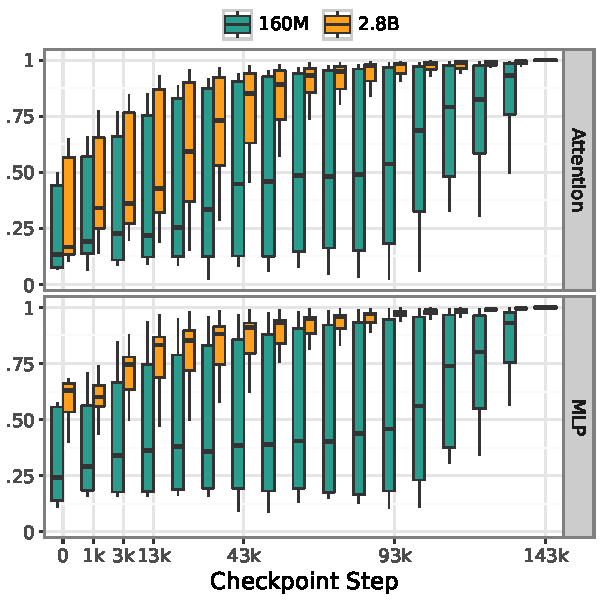
\includegraphics[width=0.54\columnwidth]{chapters/tending-towards-stability/figures/cka_main_plot.pdf}
    \caption{$\cka$ similarity (current vs.\ last checkpoint) of $\attention$ and $\mlp$ activations for Pythia \sixmil and \twobil. Distribution across layers: \integer{10}, \integer{25}, \integer{50}, \integer{75}, and \integer{90}-th percentiles per checkpoint.}
    \label{fig:cka_main_plot}
\end{wrapfigure}

Our analysis reveals systematic differences in the learning dynamics of transformer layers across model scales. We study these dynamics through two complementary lenses: the convergence behavior of layer activations and the proportional effective rank ($\per$) of layer parameters and their gradients. Together, these measures provide insight into how layers develop and utilize capacity over time during training.

Before presenting our detailed analyses, we briefly describe the structure of the main figures. \cref{fig:main-results} summarizes our core findings across three axes: (1) the convergence of activations as measured by $\cka$ similarity to final checkpoint activations (first column), (2) the proportional effective rank ($\per$) of layers' parameters (second column), and (3) the $\per$ of the corresponding parameter gradients (third column). Each row shows statistics for a different operation—$\attention$ (top) and $\mlp$ (bottom)—and each line represents the mean value across layers for five Pythia models ranging from 70M to 2.8B parameters.


\begin{figure*}[h!]
    \centering
    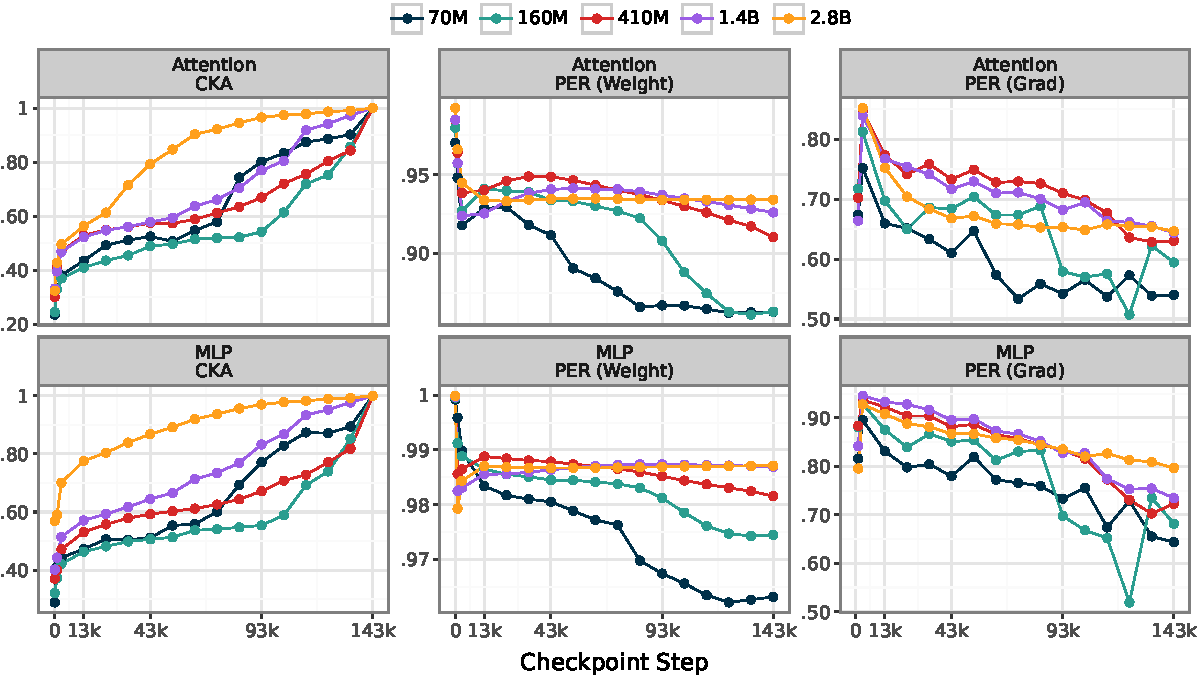
\includegraphics[width=\linewidth]{chapters/tending-towards-stability/figures/results.pdf}
    \vspace{-15pt}
    \caption{$\cka$ similarity (current vs.\ last checkpoint) of layers' activations (first column), $\per$ of layers' parameters (second column) and gradients (third column) for $\attention$ (top row) and $\mlp$ (bottom row) in Pythia \sevenmil, \sixmil, \fourmil, \onebil, and \twobil averaged (mean) across layers per each checkpoint.}
    \label{fig:main-results}
\end{figure*}



In addition to these averaged results, \cref{fig:cka_main_plot} displays the inter-quartile range of $\cka$ similarity values averaged across layers for the smallest and largest models, and \cref{fig:cka-layer-wise-lines}, \cref{fig:per_weight-layer-wise-lines}, and \cref{fig:per_grad-layer-wise-lines} provide a layer-wise breakdown of convergence and rank dynamics (for both weights and gradients), respectively. These figures allow us to distinguish aggregate trends from layer-specific behaviors and to track how each layer's representational capacity evolves during training.


\subsection{Convergence Dynamics}
\label{subsec:convergence-dynamics}

Two key findings emerge from our analysis of convergence dynamics: (1) larger models converge faster and more monotonically to their final state than smaller models, and (2) earlier layers converge faster than later layers, regardless of the model size. One important caveat to note is that when discussing convergence to a final state, we mean that the layer's activations at a given checkpoint are similar to their state at the point where we end training. This is not meant to imply that if we were to continue training a given model, the activations would remain at the same state. 

\clearpage

\begin{result}[Activations of larger models converge faster and more monotonically to their final state than those of smaller models] 
\label{result:cka}
    
As shown in the first column of \cref{fig:main-results}, $\cka$ similarity between a layer's activations at a given checkpoint and its final state rises more quickly in larger models. For instance, by 20\% of training, the $\cka$ score in \twobil reaches $\sim$0.8 for $\mlp$ and $\sim$0.7 for $\attention$, compared to values around 0.5 in \sevenmil and \sixmil. This trend reflects more rapid and stable convergence. \cref{fig:cka_main_plot} adds further evidence: across checkpoints, the interquartile range (25th to 75th percentiles) of $\cka$ similarity across layers is both narrower and higher in larger models, confirming convergence is more uniform layer-wise.

\cref{fig:cka-layer-wise-lines} provides a more granular, layer-wise view: in \twobil, many layers, particularly the earlier layers, achieve high similarity early in training, whereas in smaller models convergence is delayed and less monotonic. In smaller models, such as the \sevenmil model, some layers (e.g. 4, 5 and 6) actually not only do not converge early, but rather diverge from their final state for a period of training before becoming similar to their final state. As the size of the model increases, the number of layers that diverge from their final state for any period of training decreases.

\end{result}

\begin{result}[Activations of earlier layers converge faster, regardless of the model size]
Across model sizes, earlier layers' activations converge faster to their final state than those of later layers. As shown in \cref{fig:cka-layer-wise-lines}, the faster average convergence in larger models is due to more of their later layers converging earlier, whereas smaller models' layers only reach their final state towards the end of training. The key difference is that, in larger models, more of the later layers also converge earlier. For instance, the very final layers of the \sevenmil model in \cref{fig:cka-layer-wise-lines} only reach high similarity to their final state at the end of training, whereas the very final layers of the \twobil model reach high similarity (over 0.75) to their final state at around 50\% of training. This finding is in line with previous research that has indicated that the final layers of small models tend to degenerate late in training \citep{godey2024small}.
\end{result}
    


\clearpage

\begin{figure*}[h!]
    \centering
    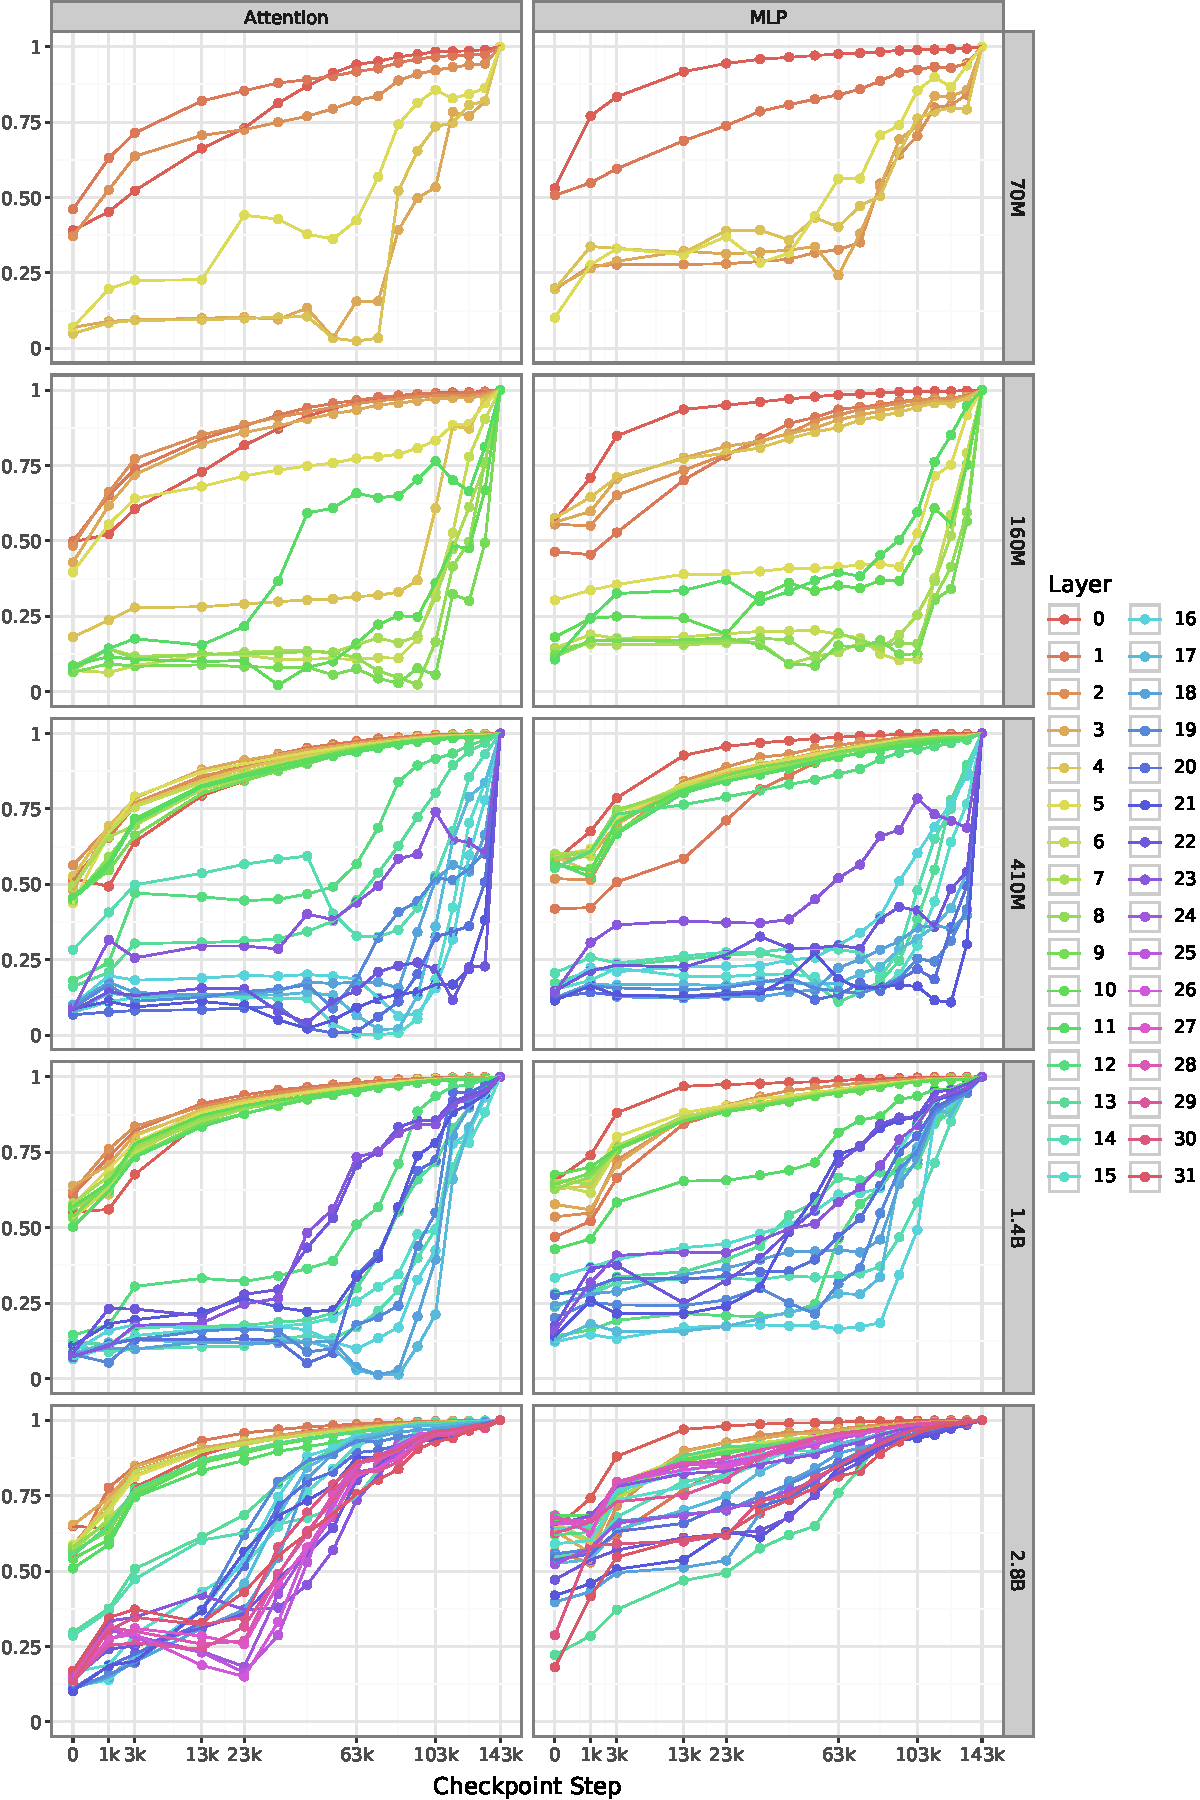
\includegraphics[width=0.9\linewidth]{chapters/tending-towards-stability/figures/cka_full_lines.pdf}
    \vspace{-5pt}
    \caption{$\cka$ similarity (current vs last checkpoint) of the activations of $\attention$ and $\mlp$ in each layer of Pythia \sevenmil, \sixmil, \fourmil, \onebil, and \twobil throughout training.}%
    \label{fig:cka-layer-wise-lines}
\end{figure*}
\clearpage

\subsection{Parameter Rank Dynamics}
\label{subsec:parameter-rank-dynamics}

Based on recent work that identifies parameter rank differences across model sizes \citep{godey2024small}, we study whether the different convergence behaviors are related to the effective rank of layers' parameters and gradients. Here, two key findings emerge: (1) parameters of layers in larger models proportionally span more dimensions than those of smaller models, and (2) parameters of layers in larger models receive gradient updates along proportionally more dimensions than those of smaller models.


\begin{result}[Parameters of layers in larger models proportionally span more dimensions] 
    \label{result:weight-effective-rank} 
    Parameters in layers of larger models span a slightly larger fraction of their available dimensions compared to smaller models, as shown in \cref{fig:main-results} (second column). 
    Moreover, the $\per$ of larger models stabilizes early, while it keeps decreasing throughout training for smaller ones. This finding is further underscored when visualizing the $\per$ for each layer, as shown in \cref{fig:per_weight-layer-wise-lines}; we observe that in smaller models the $\per$ of later layers tends to decrease over the course of training, while in larger models the $\per$ of all layers stabilizes early in training. This difference is even more pronounced in the $\per$ of these layers' gradients, as shown in \cref{fig:main-results} (third column).
    \end{result}
    
    \begin{result}[Parameters of layers in larger models receive gradient updates along proportionally more dimensions]
    \label{result}
    The $\per$ of gradients reflects the proportion of the learning signal transmitted by the gradients relative to the available parameter dimensions. In \cref{fig:main-results} (third column), we observe that throughout training gradients in larger models consistently span a larger fraction of the available dimensions, with this fraction gradually decreasing over time. In contrast, smaller models display more variability. At first glance, the averaged $\per$ of gradients in the $\attention$ layer of the \twobil model might appear to contradict the observed trend. However, this discrepancy is clarified when examining the $\per$ of gradients across individual layers, as shown in \cref{fig:per_grad-layer-wise-lines}. Once again, we observe that the $\per$ of gradients in later layers of smaller models are less stable compared to larger models. The reason the average $\per$ of gradients in the $\attention$ layer of the \twobil model is smaller than in smaller models is that, early in training, all layers of the larger model stabilize at their final values. At this stage, the stabilized layers of the larger model have lower gradient $\per$ values compared to those of smaller models, which have not yet converged. Overall, our findings suggest that layers in larger models converge both more quickly and tend to receive proportionally larger rank updates during training.
    \end{result}

\clearpage

\begin{figure*}[h!]
    \centering
    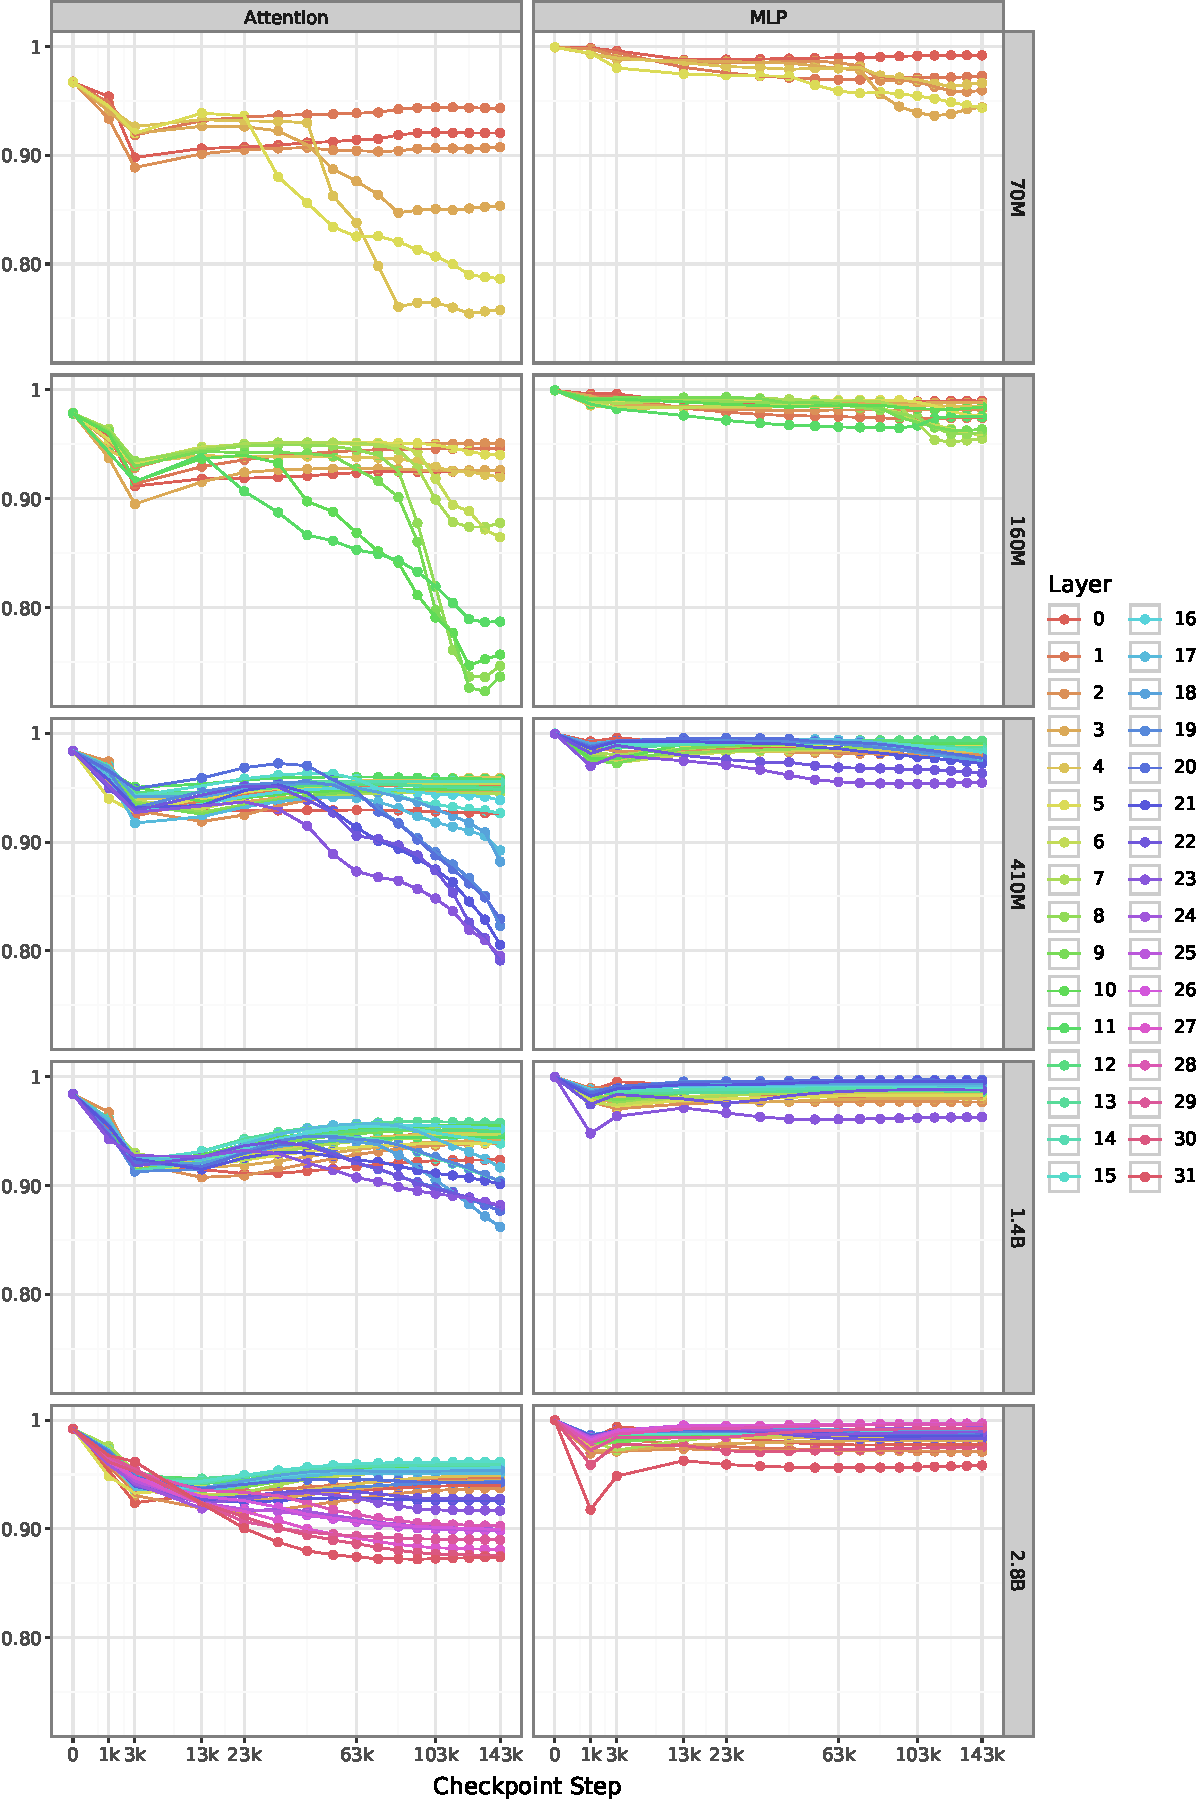
\includegraphics[width=0.9\linewidth]{chapters/tending-towards-stability/figures/per_weight_lines.pdf}
    \vspace{-5pt}
    \caption{$\per$ of the weight matrices of $\attention$ and $\mlp$ in each layer of Pythia \sevenmil, \sixmil, \fourmil, \onebil, and \twobil throughout training.}%
    \label{fig:per_weight-layer-wise-lines}
\end{figure*}
\clearpage

\begin{figure*}[h!]
    \centering
    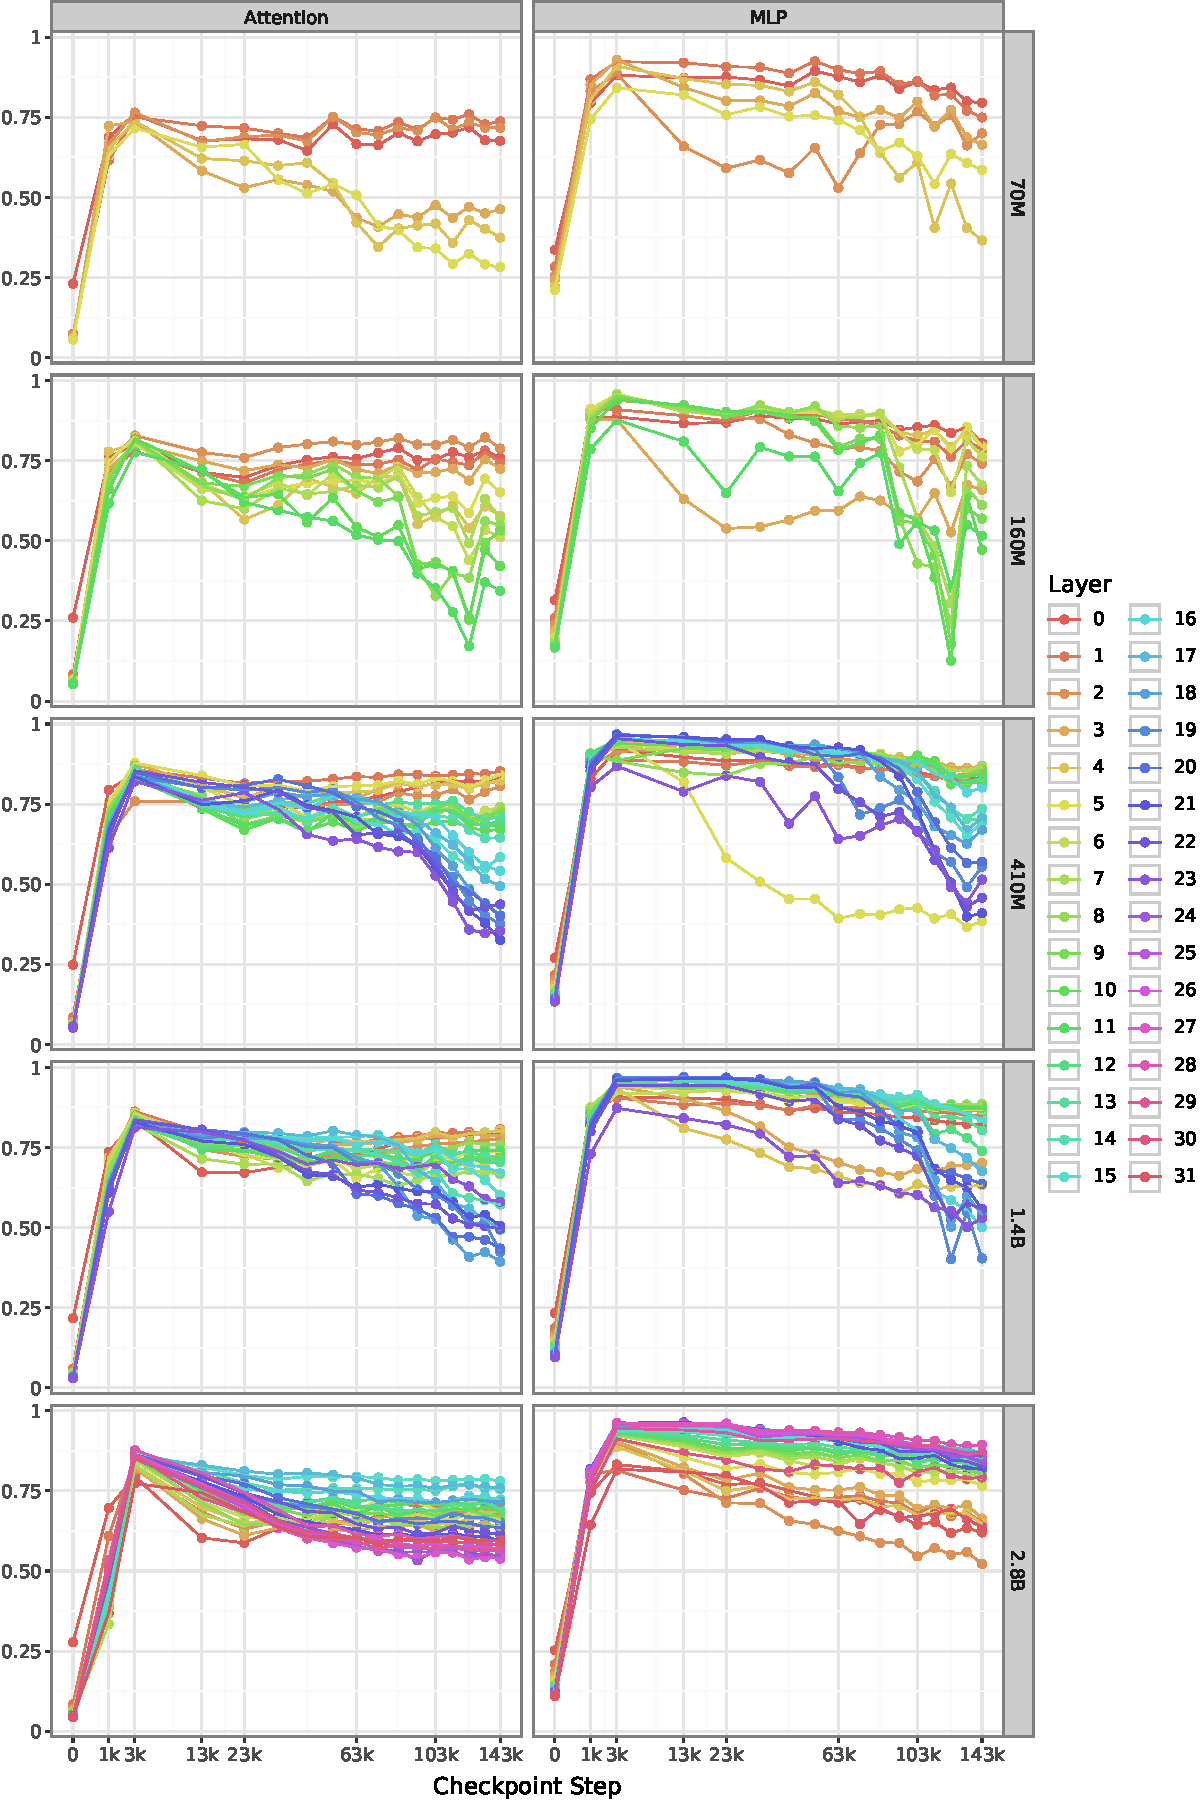
\includegraphics[width=0.9\linewidth]{chapters/tending-towards-stability/figures/per_grad_lines.pdf}
    \vspace{-5pt}
    \caption{$\per$ of the gradients of the weight matrices of $\attention$ and $\mlp$ in each layer of Pythia \sevenmil, \sixmil, \fourmil, \onebil, and \twobil throughout training.}%
    \label{fig:per_grad-layer-wise-lines}
\end{figure*}
\clearpage

\subsection{Correlation between Convergence and Rank}
\label{subsec:correlation-cka-per}

Having found key differences in the convergence and parameter rank dynamics of larger and smaller models, we now investigate whether these differences are correlated. 



% \begin{table}[!h]
%     \centering
%     \begin{tabular}{crrrr}
\toprule
 \textbf{Size} & $\attweight$  & $\nabla \attweight$ & $\mlpweight$ & $\nabla\mlpweight$\\ 
\midrule
\sevenmil  & \float[2]{1.000} & \float[2]{1.000} & \float[2]{0.632} & \float[2]{1.00} \\ 
\sixmil & \float[2]{1.000} & \float[2]{0.845} & \float[2]{0.357} & \float[2]{0.714} \\ 
\fourmil & \float[2]{0.837} & \float[2]{0.916} & \float[2]{0.192} & \float[2]{0.777} \\ 
\onebil & \float[2]{0.775} & \float[2]{0.845} & \float[2]{0.209} & \float[2]{0.641} \\ 
\twobil & \float[2]{0.728} & \float[2]{0.521} & \float[2]{0.112} & \float[2]{0.179} \\ 
\bottomrule
\end{tabular}
%     \caption{Matthew's Correlation Coefficient %($\phi$)
%     between binary variables indicating whether a given layer converges early in training and whether it maintains a stable PER of the parameters ($\vtheta$) and gradients ($\nabla\vtheta$) throughout training for both $\attention$ and $\mlp$.}
%     \label{tab:model_correlation}
% \end{table}


\begin{result}[The dynamics of the parameters' effective rank and the activations' convergence patterns are correlated]
Broadly, we find that layers with higher effective rank in both weights and gradients converge faster.
\end{result}

\begin{wrapfigure}{R}{0.5\columnwidth}
    \vspace{-20pt}
    \centering
    \begin{tabular}{crrrr}
\toprule
 \textbf{Size} & $\attweight$  & $\nabla \attweight$ & $\mlpweight$ & $\nabla\mlpweight$\\ 
\midrule
\sevenmil  & \float[2]{1.000} & \float[2]{1.000} & \float[2]{0.632} & \float[2]{1.00} \\ 
\sixmil & \float[2]{1.000} & \float[2]{0.845} & \float[2]{0.357} & \float[2]{0.714} \\ 
\fourmil & \float[2]{0.837} & \float[2]{0.916} & \float[2]{0.192} & \float[2]{0.777} \\ 
\onebil & \float[2]{0.775} & \float[2]{0.845} & \float[2]{0.209} & \float[2]{0.641} \\ 
\twobil & \float[2]{0.728} & \float[2]{0.521} & \float[2]{0.112} & \float[2]{0.179} \\ 
\bottomrule
\end{tabular}
    \captionof{table}{Matthew's Correlation Coefficient %($\phi$)
    between binary variables indicating whether a given layer converges early in training and whether it maintains a stable PER of the parameters ($\vtheta$) and gradients ($\nabla\vtheta$) throughout training for both $\attention$ and $\mlp$.}
    \label{tab:model_correlation}
\end{wrapfigure}

To measure this correlation, we first create two binary variables for each layer indicating whether (i) it converges early in training and (ii) maintains a stable $\per$ throughout training. Then, we calculate the Matthew's Correlation Coefficient between these two statistics across layers and report them in \cref{tab:model_correlation}.
Specifically, for each layer of a given model, we determine whether that layer exhibits early activations' convergence and large and stable parameters' and gradients' $\per$s (relative to other model layers) using the following heuristics: 
\begin{itemize}
    \item \textbf{Early activations' convergence.} Activations' $\cka \mathop{\geq} \float[2]{0.45}$ by the first \q{10}{\percent} of training (applies to both the $\attention$ and $\mlp$ layers).
    
    \item \textbf{Large parameters' $\per$.} Parameters' $\per \mathop{\geq} \float[2]{0.95}$ by the end of training (applies to both the $\attention$ and $\mlp$ layers).
    
    \item \textbf{Large gradients' $\per$.} We note that gradients' $\per$ slightly decreases throughout training for each model size. Rather than choosing a fixed value to determine large and stable gradients' $\per$s, we dynamically set the threshold at \q{90}{\percent} of the largest $\per$ attained by any layer at the end of training.
\end{itemize}
We observe a strong correlation for the $\attention$ layers across model sizes. For the $\mlp$ layers, the correlation with the gradients' $\per$ is strong for models up to \onebil, while the correlation with the parameters' $\per$ is strong only for the \sevenmil model. We hypothesize that this discrepancy can be explained by the fact that $\mlp$ layers have a large $\per$ throughout training across all model sizes, apart from those of the \sevenmil model. While these results are correlational, they provide a foundation for future work to test whether methods that specifically increase the PER of layers' parameters and gradients induce faster convergence of the layers' activations in small models.



% ===========
% CONCLUSIONS
% ===========
\section{Conclusion}

Our findings reveal consistent and interpretable distinctions in learning dynamics across model scales. Larger models exhibit faster and more monotonic convergence in their layer activations, and make fuller use of their representational capacity; this is evidenced by higher and more stable proportional effective ranks ($\per$) of both weights and gradients. In contrast, smaller models display delayed convergence, greater instability, and under-utilization of available capacity. These patterns suggest that part of the capability gap between small and large models may stem not from optimization failure per se, but from inefficient or truncated learning trajectories. Importantly, these insights offer actionable hypotheses: for instance, that inducing higher-rank updates or penalizing smaller effective ranks might help smaller models converge more like their larger counterparts. 

However, testing such hypotheses directly, for instance by intervening on training dynamics and re-evaluating learning behavior, is difficult in practice. Ideally, we would now like to modify the Pythia models (for example, to encourage higher effective rank early in training) and retrain them to see whether convergence patterns improve. Yet retraining Pythia is non-trivial. There are several practical limitations:

\begin{itemize}[label=\xmark]
    \item \textbf{The dataset (the Pile)} is not easily streamable in its deduplicated format, and lacks a flexible preprocessing pipeline. Simply downloading the dataset is non-trivial because it requires a large amount of disk space and a custom preprocessing script.
    \item \textbf{The model and training code requires Megatron-DeepSpeed}, which introduces heavy engineering overhead, tightly coupled dependencies, and strict hardware requirements. This also makes reading and editing the code cumbersom.
    \item \textbf{The training pipeline is distributed in Docker environments} with kubernetes for large-scale distributed training. These tools add overhead and complexity that is not necessary for small-scale research.
    \item \textbf{Checkpointing is limited to weights}, meaning that intermediate activation or gradient states of the model are missing, and difficult to recover. Further, it is not obvious how to determine the exact set of data that was seen by the model at a given checkpoint. 
    \item \textbf{Pythia checkpoints do not natively plug in with analysis libraries}, making it difficult to use existing analysis tools to study learning dynamics.
\end{itemize}

To rigorously study learning dynamics, and in particular, to test targeted training interventions, we need a framework that makes model retraining as accessible as analysis. Such a framework should:

\begin{tcolorbox}[
    colback=white,
    colframe=thesisblue,
    title=\textbf{Design Requirements for Intervention-Friendly Language Model Platforms},
    fonttitle=\bfseries,
    coltitle=white,
    arc=0mm,
    boxrule=1pt,
    left=10pt,
    right=10pt,
    top=10pt,
    bottom=10pt,
    enhanced,
    breakable
]
To effectively support intervention-based research on language model training dynamics, an ideal platform should meet the following criteria:

\begin{itemize}[label=\cmark]
    \item \textbf{Transparency and Modularity}: Fully open-source with minimal external dependencies. Code should be clean, auditable, and modular to support rapid iteration and debugging.
    
    \item \textbf{Reproducible Training and Evaluation}: Provide ready-to-use scripts and configuration files for full training and evaluation pipelines. Baselines should be reproducible with minimal tuning.
    
    \item \textbf{Streamable and Standardized Data}: Support tokenized datasets in streaming formats with built-in preprocessing, packing, and filtering. Avoid proprietary dataset formats or brittle pipelines.
    
    \item \textbf{Intermediate Checkpointing}: Include well-timed checkpoints (e.g., log-spaced or per epoch) to track learning dynamics. Checkpoints should be saved in consistent formats and compatible with analysis tools.
    
    \item \textbf{Structured Logging}: Capture training statistics, gradients, and loss metrics in structured logs (e.g., JSONL, CSV) to enable downstream learning dynamics analysis.
    
    \item \textbf{Flexible Model Configuration}: Allow for easy experimentation with model size, layer depth, attention mechanisms, and other architectural choices through config files or flags.

    \item \textbf{Automatically Plug-in With Existing Third-Party Tools}: Allow for easy integration with existing third-party tools (HuggingFace, Wandb, etc.) for analysis and visualization.

    
    \item \textbf{Lightweight Hardware Requirements}: Be optimized for small and mid-sized models to enable training and analysis on affordable GPU setups, supporting high-velocity prototyping.
\end{itemize}
\end{tcolorbox}

These requirements motivate the development of \pico: a lightweight, transparent framework designed to close the gap between training and analysis for small language models. In the next chapter, we introduce \pico and illustrate how it enables a full cycle of reproducible training, learning dynamics analysis, and hypothesis-driven interventions.




\chapter[The \picomed Framework: A Modular Framework for Hypothesis-Driven Language Model Research]{The \picosupabig Framework: A Modular Framework for Hypothesis-Driven Language Model Research}
\label{chapter:pico}

% The rapid progress of large language models (LLMs) has produced systems that excel at a wide range of natural language tasks, from reasoning and summarization to coding and multilingual translation \citep{hendrycks2021mmlu, cobbe2021gsm8k, srivastava2023bigbench}. Yet this progress has also introduced new challenges: as models grow larger and more complex, they become harder to analyze, diagnose, and refine. Developing language models as a result is typically more of an art than a science.

This chapter introduces \pico, a framework designed to transform language model development from empirical guesswork into a rigorous scientific process. \pico enables researchers to systematically observe learning dynamics, formulate testable hypotheses about model behaviour, and iterate on design choices through controlled experimentation. By bridging the gap between training and analysis in a single, accessible framework, \pico makes it possible to build language models in a more principled, hypothesis-driven manner.\footnote{Code available at: \url{https://github.com/pico-lm}.} 

Existing model development frameworks such as DeepSpeed \citep{rasley2020deepspeed} and Megatron-LM \citep{narayanan2021megatron} have focused on efficient, large-scale training. However, their emphasis on production performance and throughput often comes at the cost of transparency. Intermediate representations, gradients, and activations are rarely captured in a structured way, and instrumentation for fine-grained interpretability is typically an afterthought. As a result, researchers seeking to study learning dynamics or test training interventions face steep technical overhead.

Conversely, frameworks built for interpretability, such as TransformerLens \citep{nanda2022transformerlens}, and model suites such as Pythia \citep{biderman2023pythia} enable detailed circuit-level analysis but are mostly limited to post-hoc exploration of fully trained models. They rarely support modifications to the training process itself, and when they do, such interventions tend to be tightly coupled to specific checkpoints, architectures, or datasets. Even frameworks explicitly designed for developmental analysis, like DevInterp \citep{devinterpcode}, rely on external checkpointing pipelines and are often decoupled from model training.

To support scientific research on language models, researchers need infrastructure that both logs advanced training signals (activations and gradients) and also invites easy experimentation and modification of the training process. Crucially, this framework should be lightweight and accessible and prioritise iteration speed over engineering overhead. 

\pico is a modular, extensible framework designed to fill this gap. Built for training and analysing small-to-medium scale models (1M--1B parameters), \pico is engineered to support the scientific methodology demonstrated in the previous chapter: systematic observation, hypothesis generation, controlled experimentation, and iterative refinement. It consists of two components:

\begin{enumerate}
    \item \texttt{pico-train}, a customisable training library that simplifies training models from scratch while recording rich internal signals (weights, gradients, activations) at regular checkpoints.
    \item \texttt{pico-analyze}, a companion toolkit for querying, visualising, and analysing these signals—designed to integrate smoothly with standard scientific workflows and support user-defined metrics.
\end{enumerate}

Together, these tools make it possible to perform fine-grained, in-situ analysis of how models learn over time, test hypotheses about representation development, and prototype interventions that might improve training outcomes. This is particularly important for small models, where interpretability and efficiency are especially critical.

% \pico was built to address a concrete gap identified in the previous chapter: existing suites like Pythia offer rich insights into learning dynamics after training, but lack the flexibility and transparency needed to test interventions during training. The findings from \cref{chapter:tending-towards-stability} (e.g. the correlation between effective rank and convergence speed) generate specific, testable hypotheses that require tools for systematic experimentation. \pico provides these tools, bringing the same level of rigor to the training process as to post-hoc analysis.

The rest of this chapter is structured as follows. I begin by situating \pico within the broader ecosystem of language model training and interpretability frameworks, reviewing both large-scale production platforms and experimental research toolkits. I then describe the key architectural and design decisions behind \texttt{pico-train} and \texttt{pico-analyze}, highlighting how they support training-time experimentation. Finally, I demonstrate \pico's value through case studies that show how it enables researchers to systematically test and refine hypotheses about language model learning dynamics.

{
\renewcommand{\arraystretch}{1.25}
\setlength{\tabcolsep}{4pt}

\begin{table}[htbp]
    \centering
    \footnotesize
    \begin{tabular}{@{}p{2.7cm} p{1.7cm} p{2.4cm} p{2.3cm} p{2.3cm} p{2.2cm}@{}}
    \toprule
    \textbf{Tool} &
    \textbf{Custom \newline Training} &
    \textbf{Checkpoint \newline Support} &
    \textbf{Feature \newline Extraction} &
    \textbf{Analysis \newline Tools} &
    \textbf{Low-Budget \newline Friendly} \\
    \midrule
    \textbf{\pico} & 
    \cmark \newline Modular \newline PyTorch &
    \cmark \newline Optimizer, \newline weights \& data &
    \cmark \newline Activations \& \newline gradients &
    \cmark \newline \texttt{pico-analyze} \newline metrics &
    \cmark \newline Academic \newline GPU-scale \\

    \midrule

    TransformerLens & 
    \xmark & \xmark & \cmark & \cmark & \cmark \\

    ACDC & 
    \xmark & \xmark & \cmark & \cmark & \cmark \\

    SAELens & 
    \xmark & \xmark & \warnmark & \cmark & \cmark \\

    \midrule

    SmolLM2 & 
    \cmark & \warnmark & \xmark & \xmark & \cmark \\

    Pythia Suite & 
    \warnmark & \warnmark & \xmark & \warnmark & \cmark \\

    OLMo & 
    \cmark & \warnmark & \xmark & \xmark & \warnmark \\

    \bottomrule
    \end{tabular}

    \caption{Comparison of Pico and related frameworks for interpretability and learning dynamics. 
    \label{tab:pico_comparison} \newline
    \textbf{Legend:} \cmark = Fully supported; \warnmark = Partial; \xmark = Not supported.}
\end{table}
}

\section[Situating \picomed Among Language Model Frameworks]{Situating \picolarge Among Language Model Frameworks}
\label{sec:pico-related}

Language model research increasingly depends on infrastructure that supports both scaling up training and opening up models to analysis. As interest grows in how models acquire structure, allocate capacity, and evolve over time, researchers need frameworks that support more than just efficient training. They need transparency into the training process itself.

To understand the niche \pico fills, I situate it relative to two major categories of tools: training frameworks and analysis frameworks.
% Today's ecosystem of LLM tooling is rich but uneven. On one end are large-scale training platforms that emphasize throughput, hardware optimisation, and production readiness, these include DeepSpeed \citep{rasley2020deepspeed}, Megatron-LM \citep{narayanan2021megatron}, and MosaicML's MPT \citep{mosaic2023mpt}. On the other are interpretability toolkits that provide detailed post-hoc analysis of model internals, often at the level of neurons, circuits, or activations, such as TransformerLens \citep{nanda2022transformerlens}, ROME \citep{meng2022locating}, and ACDC \citep{conmy2023towards}. However, few systems support both perspectives simultaneously. \pico is designed to bridge this gap. It supports full training from scratch, while offering built-in mechanisms to log and analyze activations, gradients, and other internal signals throughout training. This makes it possible to study learning dynamics not only retrospectively, but as they unfold which can then inform future design choices.


\paragraph{Training Frameworks}
Large-scale systems like Megatron-LM \citep{narayanan2021megatron}, DeepSpeed \citep{rasley2020deepspeed}, and MosaicML \citep{mosaic2023mpt} are highly optimised for training massive models. They handle distributed computation and mixed-precision arithmetic efficiently, but their training pipelines are complex and often opaque. Modifying or instrumenting them to inspect model internals (let alone run repeated training interventions) can require significant effort. These frameworks are indispensable for production-scale pretraining, but ill-suited for small-scale, experiment-driven research.

In contrast, lightweight training frameworks such as NanoGPT \citep{karpathy2023nanogpt}, SmolLM2 \citep{allal2025smollm2}, TinyLlama \citep{zhang2024tinyllama}, and TinyStories \citep{eldan2023tinystories} emphasise simplicity and fast iteration. Their codebases are accessible and easy to modify, making them ideal for prototyping new ideas. However, they tend to treat training as a black box. Logging activations or inspecting weight evolution generally requires manual modification, and internal state tracking is minimal or absent. These frameworks make it easy to run experiments, but hard to measure what is happening inside.

%\pico aims to combine the best of both worlds. It is optimised for small and mid-sized models (1M--1B parameters) and is built in modular PyTorch for ease of use. But unlike most lightweight suites, it is designed from the ground up to expose model internals. It logs key training signals by default (weights, activations, gradients) and does so in structured, extensible formats. %This makes \pico not just a tool for training models, but a platform for studying how they learn.

\paragraph{Analysis Frameworks}
Where training frameworks help build models, analysis frameworks help interpret them. Recent progress in mechanistic interpretability has produced tools like TransformerLens \citep{nanda2022transformerlens}, ROME \citep{meng2022locating}, and ACDC \citep{conmy2023towards}, which allow detailed inspection of trained transformer circuits. These tools are useful for understanding among other things how attention heads specialise or how knowledge is stored and retrieved. But they are mostly post-hoc: they assume a trained model and operate over static checkpoints.

Model suites such as Pythia \citep{biderman2023pythia} and OLMo \citep{groeneveld2024olmo} provided researchers a set of pretrained models and training checkpoints to study. Rather than having to train a model from scratch, researchers can use these models to analyse the learning dynamics of a model that has already been trained, using consistent checkpoints and data. However, these frameworks are not designed to retrain models from scratch.

Complementing the frameworks above are tools like DevInterp \citep{devinterpcode}, which begin to trace how models develop during training by analysing intermediate checkpoints. This shift toward developmental interpretability has revealed that models undergo discrete representational shifts and acquire capabilities in phases \citep{hoogland2023towards, hoogland2025losslandscape}. However, all of these frameworks remain downstream of the training process; they depend on external training pipelines and cannot modify or influence the training process itself.

% Here again, \pico closes a key loop. By integrating training and analysis into the same workflow, it enables fine-grained, in-situ investigation of representational dynamics. Rather than relying on occasional checkpoints saved by another framework, \pico makes detailed logging a native part of the training loop. This allows researchers to monitor changes in capacity usage, representation similarity, or sparsity metrics in real time, and to test hypotheses by intervening directly in training.

\paragraph{Toward Integrated Research Infrastructure}
The distinctions between training and analysis frameworks have historically reflected different goals—efficiency vs. interpretability, scale vs. visibility. But to understand how language models learn, especially at small and intermediate scales, these goals need to be brought together. \pico is an attempt to unify them into a single research workflow, one that enables controlled experimentation, rapid iteration, and structured analysis without sacrificing clarity or flexibility.

\cref{tab:pico_comparison} provides a comparative summary of how \pico fits into the current landscape, alongside other commonly used frameworks. While each tool has strengths of its own, \pico is distinct in offering custom training, rich logging, and built-in analysis all in one package.

\section[\picomed]{\picolarge}

In this section I provide a concise overview of the two \pico libraries: \texttt{pico-train} and \texttt{pico-analyze}. 

\subsection{\texttt{pico-train}: A Minimalist Approach to Model Training}

\texttt{pico-train} is a lightweight, transparent framework for training small- to medium-scale language models. Unlike many existing training libraries that prioritise efficiency at the cost of clarity, \texttt{pico-train} is designed to be simple, modular, and easy to modify. This makes it a flexible foundation for experimentation in language model research.

Out of the box, \texttt{pico-train} implements \texttt{pico-decoder}, a LLaMA-style transformer \citep{touvron2023llama} that incorporates key features of modern auto-regressive language models, including Grouped Query Attention (GQA) \citep{ainslie2023gqa}, Rotary Position Embeddings (RoPE) \citep{su2024rope}, FlashAttention \citep{dao2022flashattention}, SwiGLU activations \citep{shazeer2020glu}, and RMSNorm \citep{zhang2019rmsnorm}. All components (except FlashAttention) are re-implemented from scratch in plain PyTorch \citep{paszke2017pytorch}, with an emphasis on readability and documentation. %Future iterations of \pico will introduce additional architectures, such as \texttt{pico-diffusion} and \texttt{pico-statespace} models, all adhering to the same guiding principle: every \texttt{pico-*} model must be simple, well-documented, and serve as a clear base implementation for the given model architecture.

To ensure efficient multi-GPU and distributed training, \texttt{pico-train} is built on Lightning Fabric \citep{lightning-fabric}. Lightning Fabric enables users to scale up training across multiple GPUs or nodes without introducing excessive abstractions and ensures that the core training logic remains easy to understand and modify.

A distinguishing feature of \texttt{pico-train} is its systematic checkpointing and version control system. It automatically saves:
\begin{itemize}
    \item \textbf{Model states in both PyTorch- and Hugging Face-compatible formats} \citep{huggingface}. This dual-format checkpointing enables straightforward loading with vanilla PyTorch or integration into the Hugging Face ecosystem, facilitating downstream tasks such as fine-tuning, inference, or model sharing. Researchers can thus easily plug \texttt{pico-train} outputs into existing pipelines or community projects.

    \item \textbf{Intermediate activations and gradients.} At user-defined intervals, the library gathers layerwise activations and gradients from the forward and backward passes on the current training batch. Optionally, it can also capture these metrics from a fixed evaluation batch for consistent comparisons over training. Collecting these tensors at each checkpoint provides a granular record of how representations and gradient flows evolve over time.

    \item \textbf{Evaluation results.} During training, \texttt{pico-train} records user-defined evaluation metrics (e.g., validation perplexity or accuracy) alongside model checkpoints.
\end{itemize}
\vspace{-0.2em}
All checkpoints are automatically uploaded and version-controlled on Hugging Face, ensuring that researchers can revisit any point in training to analyse how the model evolved over time. These structured checkpoints integrate seamlessly with \texttt{pico-analyze}, enabling learning dynamics research with minimal setup.

\subsection{Pretokenized Dataset: \texttt{pretokenized-dolma}}

To simplify experimentation, I also release \textbf{\texttt{pretokenized-dolma}}: a pre-tokenized, pre-chunked, and pre-shuffled version of Dolma \citep{soldaini2024dolma}, a large, open-source English dataset. This dataset removes preprocessing overhead, ensures consistency across runs, and supports streaming to reduce storage needs. Using it is optional; users can substitute their own data if they prefer. 

To prepare the \textbf{\texttt{pretokenized-dolma}} dataset, I begin by downloading the Dolma corpus and selecting a random 30\% subset. The text is then tokenised using the open-sourced \textbf{\texttt{allenai/OLMo-7B-0724-hf}} tokenizer and split into fixed-length sequences of 2049 tokens (2048 + 1 for next-token prediction). I ensure consistency across shards by chunking token streams without overlap, dropping any remainder shorter than the full sequence length.

After tokenisation and chunking, I shuffle the dataset and sample a fixed number of sequences per shard, generating 100 shards in total. To facilitate scalable loading and training, I further fine-shard the dataset into 10,000 pieces using a secondary script. These final shards are compact (78MB each), randomly shuffled, pre-tokenized, and ready for streaming via the Hugging Face datasets API. This preprocessing ensures that all models see data in a consistent order, which is critical for learning dynamics analysis. I release all of the scripts used for preprocessing data in a GitHub repository. The resulting dataset is saved as Parquet files and uploaded to a Hugging Face organisation\footnote{\url{https://huggingface.co/pico-lm}} I created under \href{https://huggingface.co/datasets/pico-lm/pretokenized-dolma}{\textcolor{blue}{\textbf{\texttt{pico-lm/pretokenized-dolma}}}}.

The design philosophy for the dataset is the same as for \texttt{pico-train}: minimalism, modularity, and transparency, that enable users to easily modify all aspects of the training pipeline. 

\subsection{\texttt{pico-analyze}: A General-Purpose Framework for Studying Learning Dynamics}

\texttt{pico-analyze} is a companion tool to \texttt{pico-train} designed to make analysing learning dynamics seamless and reproducible. It directly integrates with the checkpoints saved by \texttt{pico-train}, including model weights, optimizer states, activations, and gradients, allowing researchers to systematically compute the learning dynamics of trained models.

At its core, \texttt{pico-analyze} follows a simple abstraction: it applies metrics to components. Metrics provide quantitative insights into various aspects of model behaviour, while components define the specific model elements being analysed. This design allows for flexible and fine-grained analysis of training dynamics. 

\paragraph{Metrics.} Out of the box, \texttt{pico-analyze} supports a range of built-in metrics. These include:
\begin{itemize}
    \item \textbf{Sparsity Measures}: \textit{Gini coefficient} \citep{hurley2009gini} and \textit{Hoyer metric} \citep{hoyer2004sparsity} gauge how concentrated the values of a tensor are around zero.

    \item \textbf{Rank-Based Metrics}: \textit{Proportional Effective Rank} (defined in Chapter 6) captures a matrix's “effective dimensionality”, while \textit{Condition Number} evaluates its numerical stability.

    \item \textbf{Representation Similarity}: \textit{CKA} \citep{kornblith2019cka} and \textit{PWCCA} \citep{morcos2018pwcca} compare activation patterns across layers or checkpoints, revealing how internal representations evolve.
    
    \item \textbf{Norms}: \textit{Frobenius}, \textit{Nuclear}, and \textit{Infinity} norms measure the scale of a tensor, spotlighting issues such as vanishing or exploding parameters.
\end{itemize}

\paragraph{Components.} Metrics can be computed on different types of components, which fall into two categories: 
\begin{itemize} 
\item \textbf{Simple components}: Individual weight matrices, gradients, or activations from a single layer. 
\item \textbf{Compound components}: Higher-level structures that combine multiple model elements. One example is the OV circuit, which tracks how information flows in transformer models by combining the value projection and output projection matrices in self-attention layers \cite{elhage2021mathematical}. 
\end{itemize}

This two-step abstraction is designed for extensibility: new metrics and component types can be easily defined, allowing researchers to tailor analyses to specific hypotheses about language model learning. Note that I provide a detailed explanation of all of the metrics in \cref{chapter:analysis-background}.

\section{Usage Demonstration} 
\label{sec:usage-demonstration}

To illustrate how \pico enables rigorous, hypothesis-driven research in practice, this section walks through a minimal end-to-end workflow. Rather than simply showing how to run code, this demonstration highlights how researchers can configure, train, and analyse small models to test specific learning dynamics hypotheses. \pico forms a closed scientific loop of observation, intervention, and refinement.

\subsection{Training Models with \texttt{pico-train}}

Setting up the \texttt{pico-train} codebase requires running the following commands:

\begin{center}
    \begin{codelisting}
        git clone https://github.com/pico-lm/pico-train.git
        cd pico-train
        echo "HF_TOKEN=your_huggingface_token" >> .env
        echo "WANDB_API=your_wandb_key" >> .env
        source setup.sh
    \end{codelisting}
\end{center}

I provide a simple \verb|setup.sh| script that uses Poetry \citep{poetry} to install dependencies and configure the environment. Training a model requires only a configuration file. \texttt{pico-train} uses flexible dataclasses with sensible defaults that can be easily customised for each run. I report all of the defaults in \cref{tab:default_configs}. For demonstration purposes, I include a sample configuration file in \texttt{pico-train} that can be found under \href{https://github.com/pico-lm/pico-train/blob/main/configs/demo.yaml}{\textcolor{blue}{\texttt{configs/demo.yaml}}}.\footnote{\url{https://github.com/pico-lm/pico-train/blob/main/configs/demo.yaml}} The toy model trained by this configuration is a tiny 11M parameter model, trained for only 100 steps. Here I show an abridged version of this configuration:


\begin{center}
    \begin{configlisting}
        data:
            # dataset and dataloading configurations

        checkpointing:
            run_name: "pico-decoder-demo-run"
            save_to_hf: true
            hf_checkpoint_id:
                repo_id: "pico-lm/demo"
        
        model:
            # model and model loading configurations

        evaluation:
            # evaluation configurations

        monitoring:
            # monitoring and monitoring loading configurations
            save_to_wandb: true
            wandb:
                project: "pico-demo"
                entity: "pico-lm"
            
        training:
            # training configurations
    \end{configlisting}
\end{center}
% \begin{figure}[h!] 
%     \centering
%     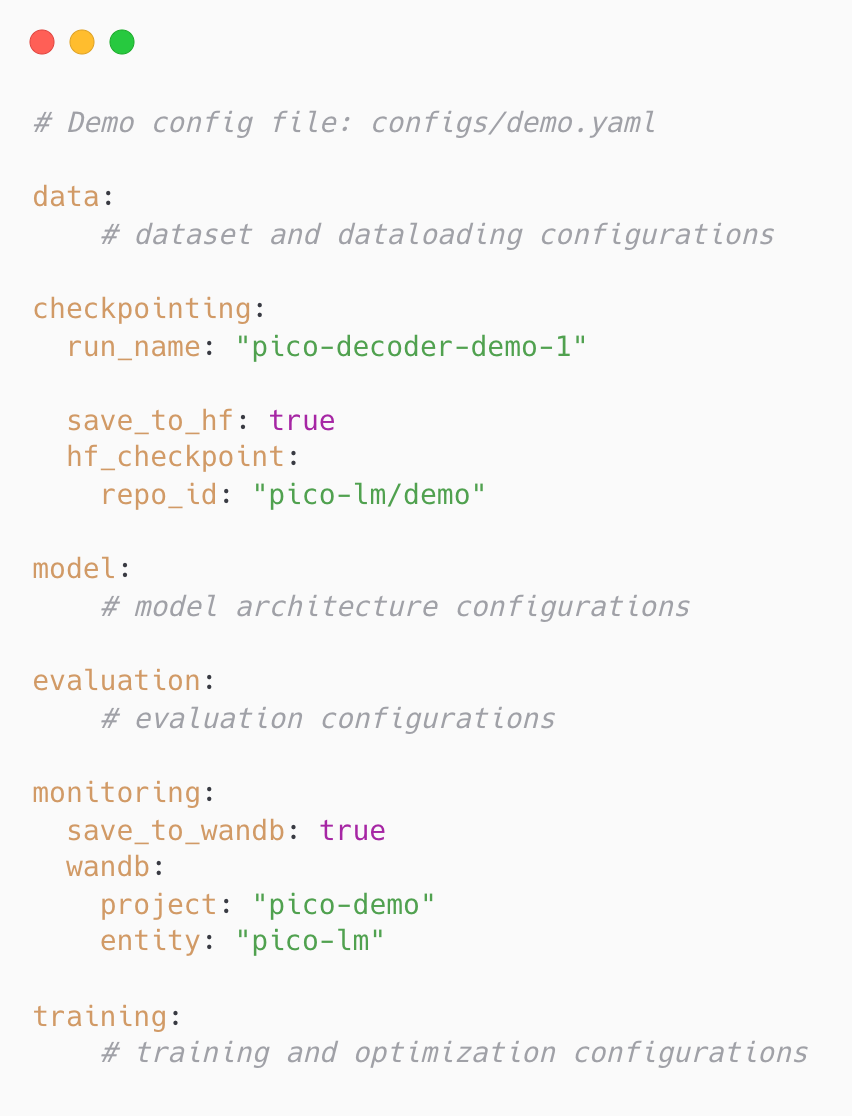
\includegraphics[width=0.7\columnwidth]{chapters/pico/figures/demo/demo_config.png}
%     \caption{The abridged demo configuration setup that we include with \texttt{pico-train}.}
%     \label{fig:demo_config}
% \end{figure}

In general, the configuration file consists of six main components, each controlling key aspects of model training. 

Using this demo configuration file, users can launch a training run as follows:

\begin{center}
    \begin{codelisting}
        poetry run pico-train --config_path configs/demo.yaml
    \end{codelisting}
\end{center}

Training will start immediately, automatically saving learning dynamics checkpoints both locally and on Hugging Face. In \cref{tab:default_configs} I report the default configuration settings used in \texttt{pico-train}; users should refer to this table when configuring their own runs.

\begin{table*}[h!]
    \centering
    \renewcommand{\arraystretch}{1.2} % Adjust row spacing
    \setlength{\tabcolsep}{8pt} % Adjust column spacing
    \footnotesize
    \begin{tabular}{|>{\centering\arraybackslash}p{3cm}|p{5cm}|p{5.5cm}|}
        \hline
        \textbf{Category} & \textbf{Parameter} & \textbf{Default Value} \\
        \hline
        \multirow{10}{*}{\textbf{Model}}  
            & Model Type & \texttt{pico\_decoder} \\
            & Hidden Dimension ($d_{\text{model}}$) & 768 \\
            & Number of Layers ($n_{\text{layers}}$) & 12 \\
            & Vocabulary Size & 50,304 \\
            & Sequence Length & 2,048 \\
            & Attention Heads & 12 \\
            & Key/Value Heads & 4 \\
            & Activation Hidden Dim & 3,072 \\
            & Normalisation Epsilon & $1 \times 10^{-6}$ \\
            & Positional Emb. Theta & 10,000.0 \\
        \hline
        \multirow{7}{*}{\textbf{Training}}  
            & Optimizer & AdamW \\
            & Learning Rate & $3 \times 10^{-4}$ \\
            & LR Scheduler & Linear w/ Warmup \\
            & Warmup Steps & 2,500 \\
            & Gradient Accum. Steps & 128 \\
            & Max Training Steps & 200,000 \\
            & Precision & BF16 Mixed \\
            %& Accelerator & CUDA \\
            %& Nodes & 1 \\
            %& Devices per Node & 1 \\
        \hline
        \multirow{3}{*}{\textbf{Data}}  
            & Dataset Name & \texttt{pretokenized-dolma} \\
            & Batch Size & 1,024 \\
            & Tokenizer & \texttt{allenai/OLMo-7B-0724-hf} \\
        \hline
        \multirow{6}{*}{\textbf{Checkpointing}}  
            & Auto Resume & True \\
            & Save Every N Steps & 1,000 \\
            %& Save to Hugging Face & False \\
            & Learning Dynamics Layers & \texttt{"attention.v\_proj",} \newline \texttt{"attention.o\_proj",} \newline \texttt{"swiglu.w\_2"} \\
            & Learning Dynamics Data & \texttt{pretokenized-paloma-tinsy} \\
        \hline
        \multirow{3}{*}{\textbf{Evaluation}}  
            & Metrics & \texttt{["paloma"]} \\
            & Eval Dataset Name & \texttt{pretokenized-paloma-tinsy} \\
            & Eval Batch Size & 16 \\
        \hline
        \multirow{3}{*}{\textbf{Monitoring}}  
            & Logging Level & INFO \\
            & Log Every N Steps & 100 \\
            %& Save to Weights \& Biases & False \\
        \hline
    \end{tabular}
    \caption{Default configuration settings used in \texttt{pico-train}, organised by configuration category.}
    \label{tab:default_configs}
\end{table*}

\subsection{Analysing Models with \texttt{pico-analyze}}


Once training is complete, users can inspect various aspects of the model's learning dynamics using \texttt{pico-analyze}. The setup process mirrors that of \texttt{pico-train}, making it simple to switch between training and analysis within the same workflow. \texttt{pico-analyze} works directly on the structured checkpoints saved by \texttt{pico-train}, computing metrics on model weights, gradients, and activations to provide insights into how the model evolves during training. To streamline experimentation, it uses a YAML-based configuration system that lets users specify which layers, metrics, and training steps to analyse. I include a complete sample configuration at \href{https://github.com/pico-lm/pico-analyze/blob/main/configs/demo.yaml}{\textcolor{blue}{\texttt{configs/demo.yaml}}}\footnote{\url{https://github.com/pico-lm/pico-analyze/blob/main/configs/demo.yaml}} within the \texttt{pico-analyze} repository.

To illustrate how this works in practice, one part of the demonstration configuration uses Centered Kernel Alignment (CKA) to test how much the model's internal representations change over training. As discussed in \cref{chapter:analysis-background}, Centered Kernel Alignment (CKA) is a well-established metric for comparing the similarity of activations between layers, checkpoints, or even different models. In this demonstration, I use CKA to track the convergence of the OV circuit at the first and last layers of the model. In general, I would expect the CKA score to begin at a value close to 0 and increase over time as the representations converge to their final state. However, since this toy example only trains for 100 steps, I hypothesise that there should be little representational change, and the CKA score should remain relatively high. This illustrates how users of Pico can turn a vague question such as “are the representations of my model changing?” into a quantitative hypothesis.

Below is an abridged YAML configuration that specifies this CKA analysis:

\begin{center}
\begin{configlisting}
    metrics:
    - metric_name: cka # Centered Kernel Alignment
      target_checkpoint: 100
      data_split: "val"
      components: 
        - component_name: ov_circuit
          data_type: "activations"
          layer_suffixes: 
            output_layer: "attention.o_proj"
            value_layer: "attention.v_proj"
          layers: [0,11]

\end{configlisting}
\end{center}

As expected, when I inspect the automatically generated plots (see \cref{fig:demo_full_run}), I see that the CKA similarity changes very little between the start and end of training (top left plot); at the start of training, the representations in both layers are already over 96\% similar to their final representations. This confirms that the toy model has barely begun to learn meaningful representations and highlights the obvious next step: train the model for longer. While this insight is trivial in a toy example, the same process generalises to larger models and more complex training regimes. In the subsequent section, I illustrate this through two more advanced case studies. The takeaway is that this hypothesis-driven loop (define a question, run the experiment, iterate on model design) can be scaled up to iteratively develop better language models.

\begin{figure}[t]
    \centering
    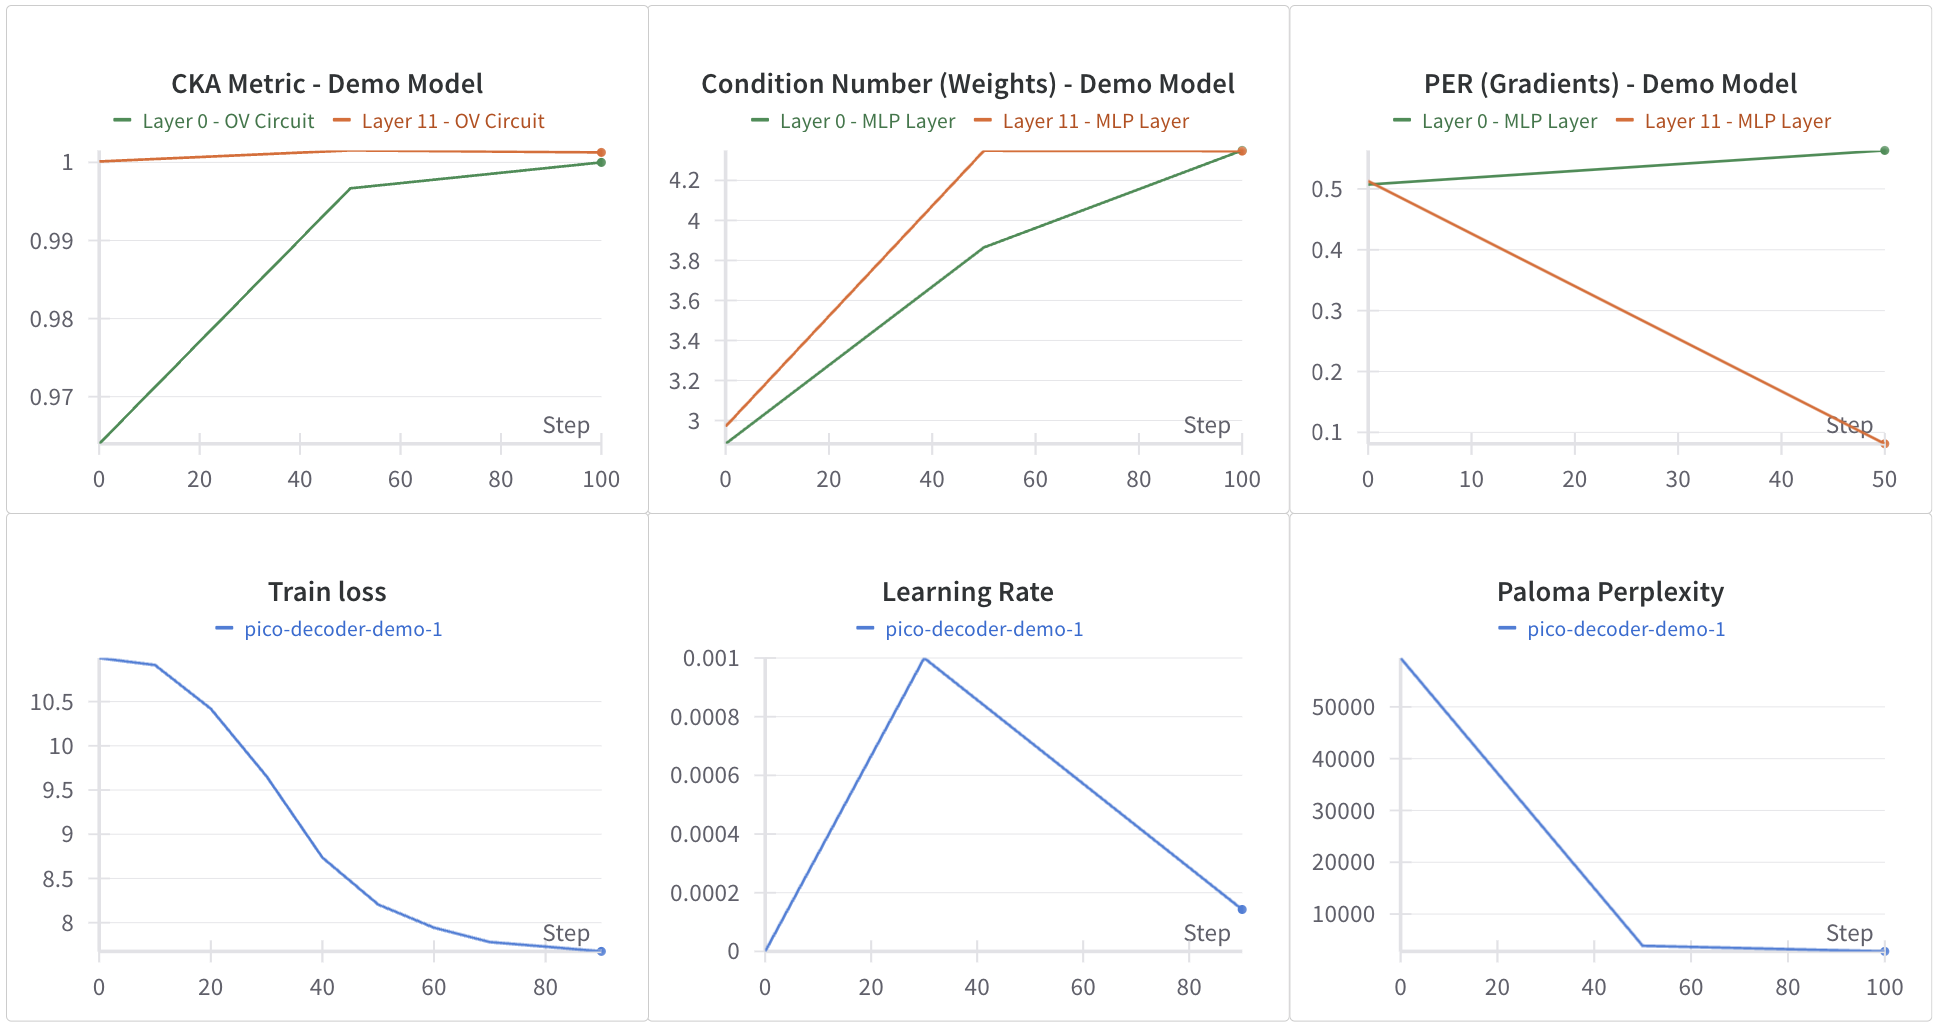
\includegraphics[width=0.9\textwidth]{chapters/pico/figures/demo_full_run.png}
    \caption{Sample analysis output of a dummy model trained using \texttt{pico-train} and analysed with \texttt{pico-analyze}. The top row illustrates some sample metrics computed by \texttt{pico-analyze} on the dummy model that was trained for 100 steps using \texttt{pico-train}, the bottom row shows training logs.}
    \label{fig:demo_full_run}
\end{figure}

In general, users can easily adapt these configuration files to test different metrics, components, or hypotheses. The full list of built-in metrics is provided in \cref{tab:pico_analyze_metrics}.

With a configuration file in place, launching an analysis is done as follows:

\begin{center}
    \begin{codelisting}
    poetry run pico-analyze
        --config_path configs/demo.yaml
        --repo_id pico-lm/demo
        --branch pico-decoder-demo-1
    \end{codelisting}
\end{center}

This command runs the specified analysis directly on the checkpoints uploaded by \texttt{pico-train}, using the given \verb|repo_id| and \verb|branch| to locate the training run. Results can be stored locally or automatically logged to Weights \& Biases (wandb) \citep{wandb} for comparison and visualisation.

By integrating seamlessly with \texttt{pico-train}, \texttt{pico-analyze} provides a structured, reproducible workflow for studying learning dynamics which inform model design choices.

\begin{table*}[h!]
    \centering
    \renewcommand{\arraystretch}{1.2} % Adjust row spacing
    \setlength{\tabcolsep}{4pt}
    \footnotesize
    \begin{tabular}{|p{4cm}|p{7.2cm}|p{1.9cm}|p{1.7cm}|}
        \hline
        \textbf{Metric} & \textbf{Description} & \textbf{Data Type} & \textbf{Category} \\
        \hline
        \hline
        \textbf{CKA \newline (Centered Kernel \newline Alignment)} \citep{kornblith2019cka} &  
        Measures similarity between activations at different checkpoints using kernel methods to track representation evolution. & Activations & \textbf{Similarity} \\
        \hline
        \textbf{PWCCA \newline (Projection-Weighted \newline CCA)} \cite{morcos2018pwcca} & 
        Measures activation similarity across training, emphasising important components via projections. & Activations & \textbf{Similarity} \\
        \hline
        \hline
        \textbf{Condition Number} &  
        Computes the ratio of largest to smallest singular value, indicating sensitivity to small input changes. & Weights\newline Activations\newline Gradients & \textbf{Rank} \\
        \hline
        \textbf{PER \newline (Proportional Effective Rank)} (Chapter 6) &  
        Measures entropy of normalised singular values to estimate effective parameter usage. & Weights\newline Gradients & \textbf{Rank} \\
        \hline
        \hline
        \textbf{Gini \newline Coefficient} \citep{hurley2009gini} &  
        Measures sparsity via inequality in the distribution of weights, activations, or gradients. & Weights\newline Activations\newline Gradients & \textbf{Sparsity} \\
        \hline
        \textbf{Hoyer's \newline Sparsity} \citep{hoyer2004sparsity} &  
        Measures sparsity using the ratio of L1 to L2 norms. & Weights\newline Activations\newline Gradients & \textbf{Sparsity} \\
        \hline
        \hline
        \textbf{Norm} &  
        Uses Frobenius, Nuclear, or Infinity matrix norms to quantify magnitude. & Weights\newline Activations\newline Gradients & \textbf{Norm} \\
        \hline
    \end{tabular}
    \caption{Overview of built-in metrics in \texttt{pico-analyze}. \textbf{Data Types} indicates on what types of checkpoint data the metrics can be applied. The \textbf{Category} column classifies metrics based on their primary purpose.}
    \label{tab:pico_analyze_metrics}
\end{table*}

\section{Case Studies}

I illustrate how \pico enables systematic, hypothesis-driven experimentation through two case studies: (1) meta-learning pre-training, (2) low-rank adapter pre-training. In each of these examples, I demonstrate demonstrate the cycle of implementation, analysis, and hypothesis refinement.

\subsection{Meta-Learning Pre-Training}

Model-Agnostic Meta-Learning (\citealp[MAML]{finn2017maml}) trains models to adapt quickly by alternating between short bursts of task-specific learning and a global update that improves generalisation. This setup encourages models to find initialisation points that adapt well to new tasks. While MAML is typically used for fine-tuning, I follow prior work \citep{bansal2020smlmt, li2021semisupervised} in applying it during pretraining.%, using synthetic token classification tasks.


\paragraph{Implementation} I implemented MAML in \texttt{pico-train} by adding a lightweight inner loop that updates a classification head on masked token tasks, followed by a meta-update to the full model. \texttt{pico-train} automatically handles distributed GPU synchronisation, requiring no changes to \pico's core training logic.

\begin{figure}[h!]
    \centering
    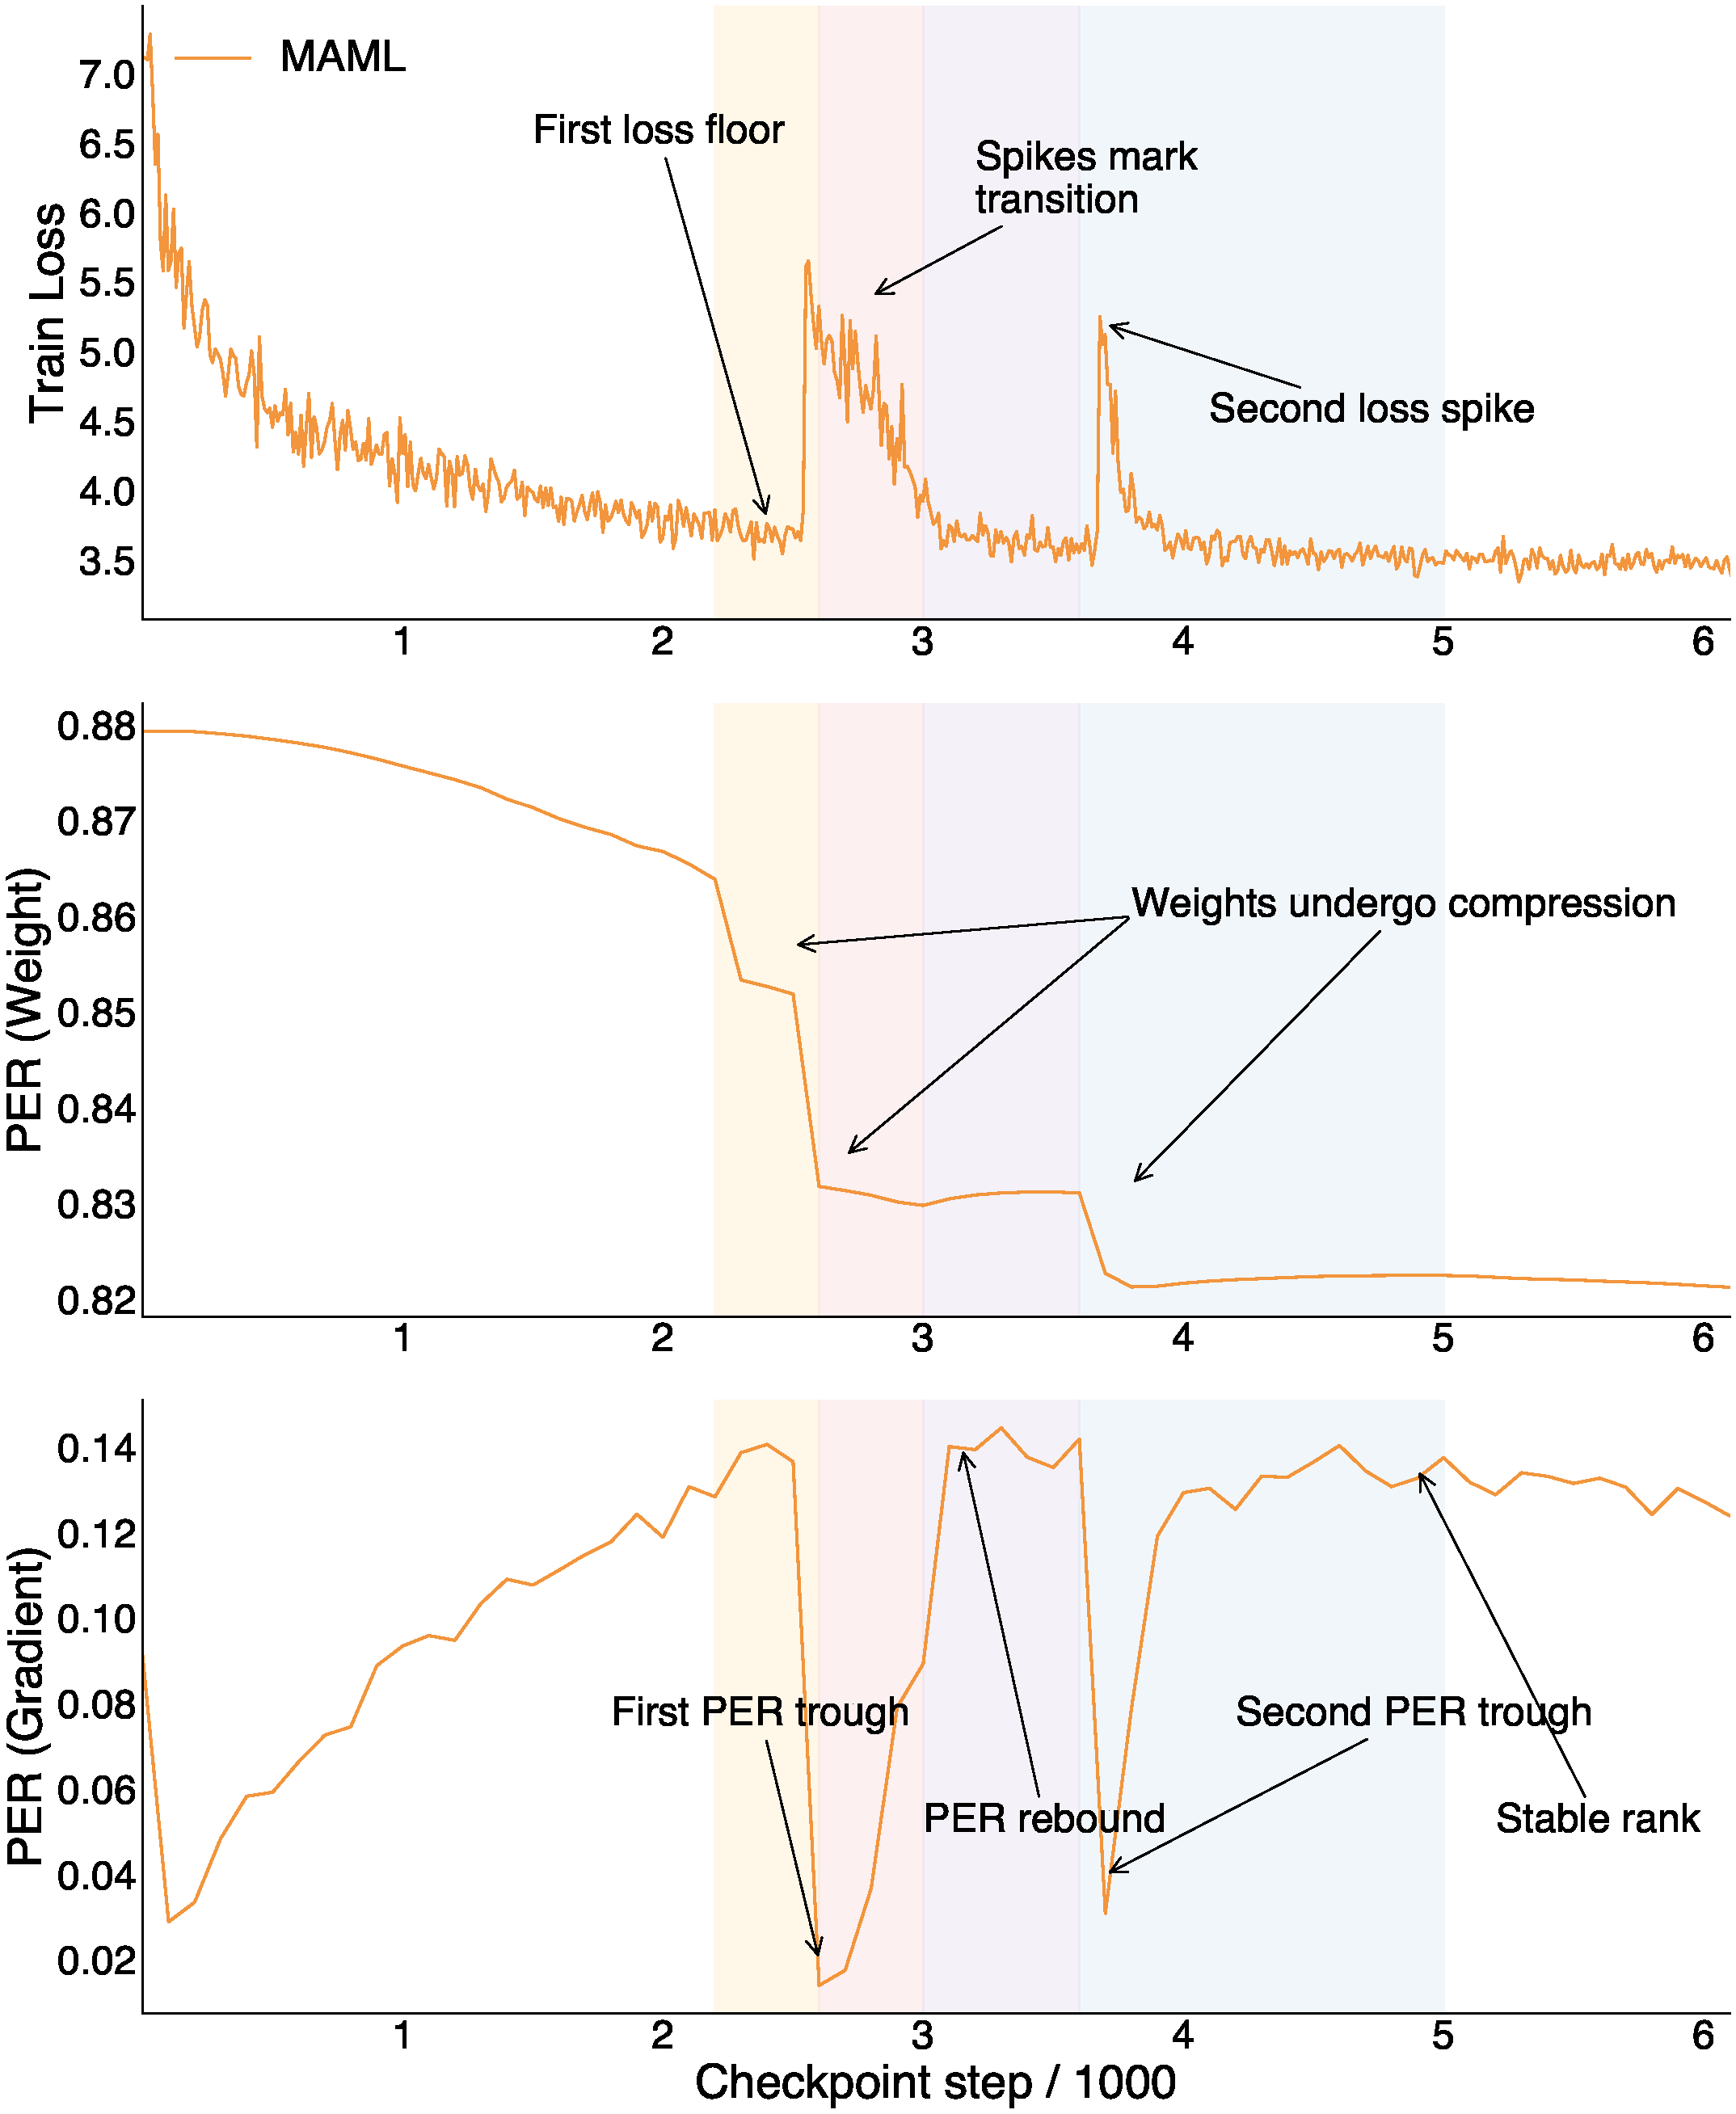
\includegraphics[width=0.6\textwidth]{chapters/pico/figures/maml-example.pdf}
    \caption{Training dynamics under MAML.
    \textbf{Top to bottom:} Training loss and proportional effective rank (PER) of weights and gradients.
    Sharp drops in PER align with spikes in loss. Shaded regions correspond to different observed phases in training. 
    }
    \label{fig:maml_example}
\end{figure}


\paragraph{Analysis} I evaluate MAML on Paloma perplexity and observe consistent 4-15\% gains over standard pretraining. To better understand this improvement, I analyse the proportional effective rank (PER) (defined in Chapter 6) of both weights and gradients over time. PER captures the dimensionality of a tensor's signal. In meta-learning, one concern is that inner-loop updates may overly constrain model updates to a low-dimensional subspace, potentially limiting generalisation. As shown in \cref{fig:maml_example}, I observe synchronised troughs in PER and spikes in both loss and perplexity. This suggests that inner-loop updates temporarily compress the model's capacity into a low-rank subspace before the outer-loop update restores variance and expressivity.


\paragraph{New Hypothesis and Next Steps}
These results support the hypothesis that MAML's learning dynamics involve cycles of compression and recovery. This raises concrete follow-up questions: could adjusting the inner-loop learning rate reduce excessive compression? Would alternative meta-learning schedules or task mixes stabilise the representational space more effectively? Using Pico's modular training and built-in logging, these variants can be tested with minimal friction. By comparing learning dynamics and outcomes across runs, researchers can refine their design choices in a reproducible, hypothesis-driven loop.% — illustrating Pico’s role as a practical sandbox for systematic small LM research.

\subsection{Low-Rank Adapter Pre-Training}

ReLoRA \citep{lialin2023relora} adapts LoRA \citep{hu2021lora}, a fine-tuning technique that freezes pretrained weights and injects trainable low-rank matrices, into the pretraining loop. In theory, this could provide a sample-efficient way to train large models by constraining updates to a low-rank subspace. %However, its impact on pretraining stability remains poorly understood.

\paragraph{Implementation} I incorporate ReLoRA into \texttt{pico-train} by adding a lightweight wrapper around attention and MLP weight matrices, and by modifying the learning rate schedule to handle periodic resets. I evaluated the model on BLiMP \citep{warstadt2020blimp}, which I configured via a single config entry. % and required minimal code modification. 

\begin{figure}[h!]
    \centering
    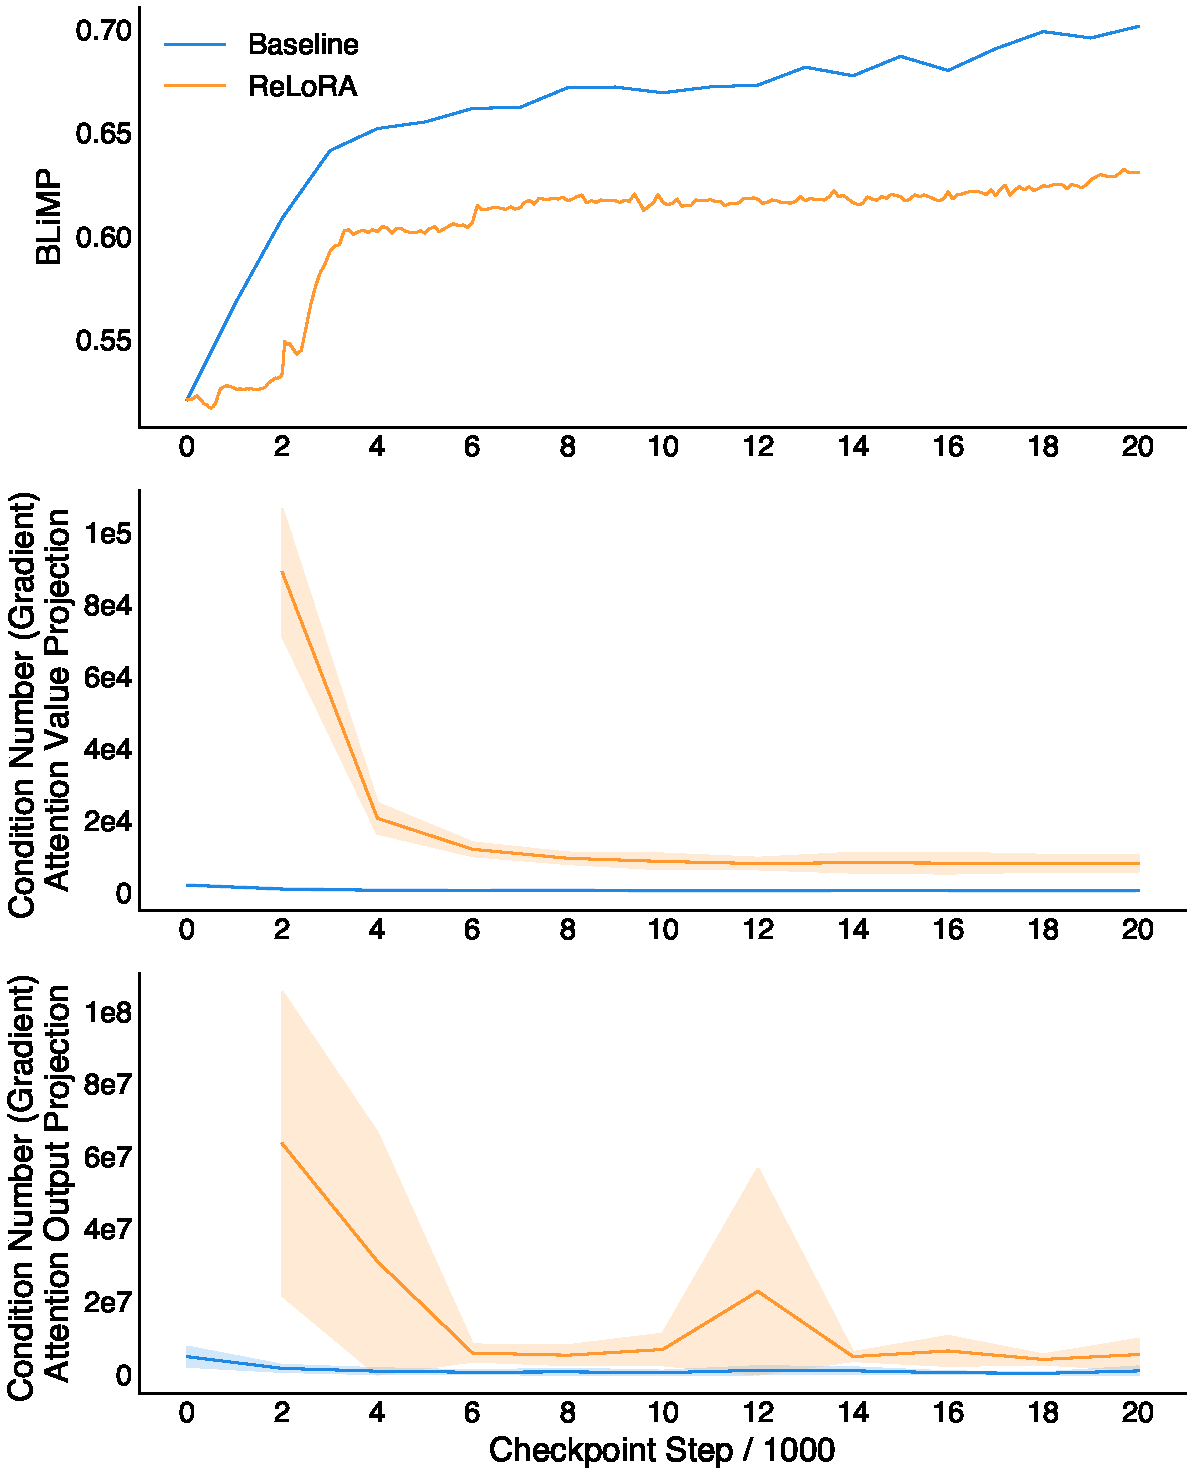
\includegraphics[width=0.6\textwidth]{chapters/pico/figures/relora-example.pdf}
    \caption{Training dynamics under ReLoRA.
    \textbf{Top to bottom:} BLiMP accuracy over time, averaged condition numbers of the gradient updates for the attention value and output projection matrices. Condition number shows wide inter-layer variance.
    }
    \label{fig:relora_example}
\end{figure}

\paragraph{Analysis} I find that ReLoRA surprisingly underperforms standard pretraining on BLiMP (see \cref{fig:relora_example}, top) \citep{warstadt2020blimp}. To investigate this, I analyse the condition numbers of the gradient updates across layers and training checkpoints. This metric reflects how sensitive gradient-based updates are to numerical instability, a relevant concern for methods like ReLoRA that repeatedly project updates into a low-rank subspace. As shown in \cref{fig:relora_example} (bottom), ReLoRA gradients are substantially more ill-conditioned and exhibit high inter-layer variance. 

% If the optimization geometry becomes poorly conditioned, learning can become more erratic.

\paragraph{New Hypothesis and Next Steps}
This pattern suggests that repeated low-rank resets may amplify gradient instability, undermining ReLoRA's intended efficiency gains. Several next steps follow naturally: for example, adding layerwise condition number regularisation, adjusting the rank dynamically, or modifying the reset schedule to reduce instability. Because \texttt{pico-train} and \texttt{pico-analyze} modularise core components and log detailed in-situ signals, researchers can test these changes quickly, track their effects on gradient stability, and iterate systematically. This demonstrates \pico's value as a scientific sandbox for implementing, analysing, and refining design choices in the small LM regime.


\section{Pico Model Suite}

In addition to releasing the \texttt{pico-train} and \texttt{pico-analyze} tools, I also train a suite of \textbf{\texttt{pico-decoder}} models at various scales using \texttt{pico-train}, all of which are open-sourced on the Hugging Face organisation.\footnote{\url{https://huggingface.co/pico-lm}} These models range from 11M to 570M parameters, with plans to extend up to 1B, and serve both as evaluations of the training pipeline and as testbeds for research on scaling laws and interpretability. I provide a comparison of these models in \cref{tab:pico-decoder-configs}.

\begin{table}[h!]
    \centering
    \renewcommand{\arraystretch}{1.2}
    \begin{tabular}{|p{0.30\textwidth}||p{0.13\textwidth}|p{0.13\textwidth}|p{0.13\textwidth}|p{0.13\textwidth}|}
    \hline
    \multicolumn{5}{|c|}{\textbf{Pico-Decoder Model Comparison}} \\
    \hline
    \textbf{Attribute} & \texttt{tiny} & \texttt{small} & \texttt{medium} & \texttt{large} \\
    \hline
    Parameter Count & 11M & 65M & 181M & 570M \\
    Hidden Dimension ($d_{\text{model}}$) & 96 & 384 & 768 & 1536 \\
    Feed-forward Dim & 384 & 1536 & 3072 & 6144 \\
    Training Time (50K steps) & 10d 9h & 15d 6h & 17d 15h & 23d 16h \\
    \hline
    \end{tabular}
    \vspace{0.5em}
    \caption{Comparison of \texttt{pico-decoder} model variants trained with default \texttt{pico-train} configurations. Except for hidden and feed-forward dimension, all models share the training settings detailed in \cref{tab:default_configs}. Models are trained for 125,000 total training steps on 16 NVIDIA A100-SXM4-80GB GPUs.}
    \label{tab:pico-decoder-configs}
    \end{table}

Each model is trained for 125,000 steps (covering 250B tokens) on the open-sourced \textbf{\texttt{pretokenized-dolma}} dataset. I evaluate the final model checkpoints on the Paloma benchmark \citep{magnusson2024paloma}, HellaSwag \citep{zellers2019hellaswag}, Arc-Easy \citep{clark2018arc} and Truthful QA \citep{lin2022truthfulqa}, comparing performance against established decoder models. As shown in \cref{tab:model_benchmarks}, the models achieve comparable results to Pythia and OPT models, despite running on an academic-level compute budget (4 nodes of 4 A100s each). This illustrates that although simple and minimal, \texttt{pico-train} is able to efficiently train models that are competitive with state-of-the-art models of the same scale.

\begin{table*}[htbp!]
    \centering
    \renewcommand{\arraystretch}{1.1}
    \setlength{\tabcolsep}{6pt}
    \small
    \begin{tabular}{lcccccc}
    \hline
    \textbf{Family} & \textbf{Size} & \textbf{\#Tokens} &
    \textbf{Paloma$\;\downarrow$} &
    \textbf{HellaSwag$\;\uparrow$} &
    \textbf{ARC-Easy$\;\uparrow$} &
    \textbf{TruthfulQA$\;\uparrow$} \\
    \hline\hline
    
    \textbf{\pico} & 11M  & 250B & 136.17 & 25.62 & 32.79 & 51.75 \\
                   & 65M  & 250B &  42.24 & 27.25 & 38.22 & 46.13 \\
                   & 181M & 250B &  30.08 & 30.69 & 44.65 & 41.85 \\
                   & 570M & 250B &  22.96 & 37.33 & 48.99 & 36.33 \\
    \hline
    
    \textbf{Pythia} & 14M  & 300B &  86.64 & 26.15 & 31.31 & 50.14 \\
                    & 70M  & 300B &  43.76 & 27.56 & 36.23 & 47.02 \\
                    & 160M & 300B &  29.96 & 30.26 & 43.73 & 44.51 \\
                    & 410M & 300B &  20.55 & 40.55 & 52.10 & 41.23 \\
    \hline
    
    \textbf{OPT}    & 125M & 300B &  27.22 & 31.33 & 43.48 & 42.89 \\
                    & 350M & 300B &  20.91 & 36.66 & 44.06 & 41.01 \\
    \hline
    \end{tabular}
    \caption{Performance of small-scale language models on four benchmarks.
    Lower is better for Paloma perplexity ($\downarrow$); higher is better for
    HellaSwag, ARC-Easy, and Truthful QA accuracies ($\uparrow$).}
    \label{tab:model_benchmarks}
    %\vspace{-0.5cm}
\end{table*}

\section{Conclusion}

% We introduce \pico, a modular framework for training and analyzing small to medium-scale language models. \texttt{pico-train} provides a minimal yet flexible environment for training language models that emphasises transparency and checkpointing for learning dynamics research. \texttt{pico-analyze} then uses these checkpoints to facilitate a broad set of learning dynamics analyses including model convergence patterns, sparsity, and rank dynamics.

% In addition, we presented the \pico Model Suite, a collection of  \textbf{\texttt{pico-decoder}} models ranging from 11M to 570M parameters, with future plans to scale to 1B+. These models are trained under controlled conditions, supporting research on scaling laws and representation learning.

% By bridging training and analysis in a lightweight, extensible framework, \pico lowers the barrier for studying language model learning dynamics. Future work will expand the model suite and integrate advanced interpretability tools, further enhancing its utility for rigorous and reproducible research.

In this chapter, I introduced \pico, a modular framework designed to transform language model development from empirical guesswork into a more rigorous, hypothesis-driven scientific process. By integrating transparent, checkpoint-rich training (\texttt{pico-train}) with systematic, reproducible analysis (\texttt{pico-analyze}), \pico bridges the gap between building models and understanding how they learn.

Unlike traditional frameworks that treat training and interpretability as separate, \pico combines them in a single, lightweight toolkit. This enables researchers to observe learning dynamics as they unfold, formulate concrete hypotheses about model behaviour, and test interventions in situ. The case studies and demonstration workflow show how this integrated loop makes language model research more principled and accessible.

The \pico Model Suite further supports this goal by providing open, reproducible checkpoints that serve as testbeds for scaling laws and interpretability research. By lowering the technical barriers to developmental analysis, \pico empowers researchers to study representation formation, capacity allocation, and training stability without requiring industrial-scale compute.

Looking ahead, my goal is to expand \pico with additional architectures and more analysis tooling to make language model research more systematic, transparent, and reproducible.


\vspace{1em}
For convenience, I provide links to the \pico Model Suite, the \pico GitHub repository, the \pico website, and the \pico demo video.

\begin{center}
    \begin{tblr}{
      colspec = {X[c] X[c] X[c] X[c]},
      colsep = 4pt,
      stretch = 0
    }
      \parbox{3.6cm}{
        \centering
        \raisebox{-0.4em}{
\includegraphics[width=1.9em]{chapters/pico/figures/assets/huggingface-logo.png}}\\
        {\footnotesize\href{https://huggingface.co/pico-lm}{\textcolor{blue}{huggingface.co/pico-lm}}}\\
        {\tiny (Apache 2.0)}
      }
      &
      \parbox{3.2cm}{
        \centering
        \raisebox{-0.1em}{
\includegraphics[width=1.5em]{chapters/pico/figures/assets/github-logo.png}}\\
        {\footnotesize\href{https://github.com/pico-lm}{\textcolor{blue}{github.com/pico-lm}}}\\
        {\tiny (Apache 2.0)}
      }
      &
      \parbox{3.2cm}{
        \centering
        \vspace{-0.5cm}
        \raisebox{-0.2em}{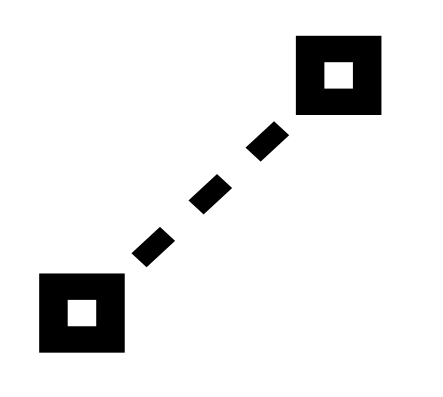
\includegraphics[width=1.4em]{chapters/pico/figures/assets/pico-tiny-logo.png}}\\
        {\footnotesize\href{https://www.picolm.io/demo-paper}{\textcolor{blue}{picolm.io}}} \\
        { }
      }
      &
      \parbox{3.2cm}{
        \centering
        \vspace{-0.5cm}
        \raisebox{-0.2em}{
\includegraphics[width=1.5em]{chapters/pico/figures/assets/youtube-logo.png}}\\
        {\footnotesize\href{https://youtu.be/llRUKwqMah4?si=F4Ol8P5Tj2ZQB7Fm}{\textcolor{blue}{Demo Video}}} \\
      }
    \end{tblr}
\end{center}





\chapter{Concluding Remarks}

Lfg this is the ending


%%%%%%%%%%%%%%%%%%%%%%%%%%%%%%%%%%%%%%%%%%%%%%%%%%%%%%%%%%%%%%%%%%%%%%%%%%%%%%%%
%% References:
%%
% If you include some work not referenced in the main text (e.g. using \nocite{}), consider changing "References" to "Bibliography".
%

% \renewcommand to change default "Bibliography" to "References"
\renewcommand{\bibname}{References}
\cleardoublepage
\phantomsection
\addcontentsline{toc}{chapter}{References}
\bibliographystyle{plainnat}
\bibliography{thesis}


%%%%%%%%%%%%%%%%%%%%%%%%%%%%%%%%%%%%%%%%%%%%%%%%%%%%%%%%%%%%%%%%%%%%%%%%%%%%%%%%
%% Appendix:
%%

\appendix


%%%%%%%%%%%%%%%%%%%%%%%%%%%%%%%%%%%%%%%%%%%%%%%%%%%%%%%%%%%%%%%%%%%%%%%%%%%%%%%%
%% Index:
%%
\printthesisindex

\end{document}